\tocless\chapter{Auswertung Videos}\label{appendix:a}
\section{Video 01}
\begin{figure}[H]
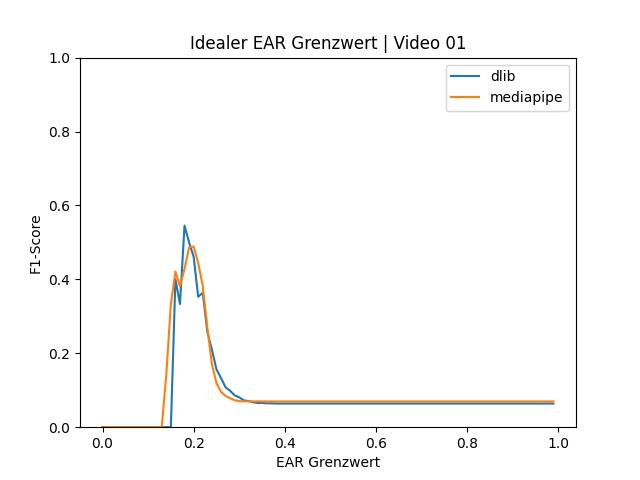
\includegraphics[width=0.7\linewidth]{appendix/01_f1-score-blink.jpg}
\caption{Ergebnisse der Bestimmung des idealen EAR-Grenzwerts für Video 01.}
\end{figure}

\begin{figure}[H]
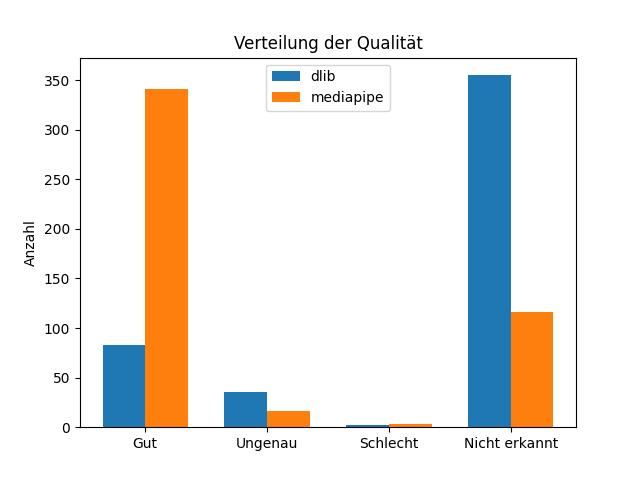
\includegraphics[width=0.7\linewidth]{appendix/01_bar-quality.jpg}
\caption{Aufteilung der Gesichtserkennungsqualität von Video 01.}
\end{figure}

\begin{table}[H]
\centering
\begin{tabular}{l|l|c c |c}
\toprule
\textbf{Gesichtserkennung} & \textbf{Blickrichtung} & \textbf{Seitenlänge} $\hitthresholdsize$ & \textbf{Verschiebung} $\hitthresholdposition$ & \textbf{F1-Score} \\ 
\midrule
\multirow{4}*{dlib}& ETH-XGaze & 0,133 & 0,01 & 0,952  \\ 
& Gaze360 & 0,296 & 0,035 & 0,952 \\ 
& MPIIFaceGaze & 0,041 & -0,039 & 0,826  \\ 
& Kopfrotation & 0,235 & 0,218 & 0,786  \\ 
\hline\multirow{4}*{MediaPipe}& ETH-XGaze & 0,122 & -0,002 & 0,983  \\ 
& Gaze360 & 0,265 & 0,035 & 0,872 \\ 
& MPIIFaceGaze & 0,031 & -0,039 & 0,57  \\ 
& Kopfrotation & 0,194 & 0,218 & 0,863  \\ 
\bottomrule\end{tabular}
\caption{Ergebnis des Hyperparameter-Tunings für die Zone speziell für Video 01.}
\label{tab:appendix:01:local}
\end{table}
\begin{table}[H]
\centering
\begin{tabular}{l|l|c c c c|c c|c}
\toprule
\textbf{Gesichtserkennung} & \textbf{Blickrichtung} & $TP$ & $TN$& $FP$ & $FN$ & \textbf{Precision} & \textbf{Recall} & \textbf{F1-Score} \\ 
\midrule
\multirow{4}*{dlib}& ETH-XGaze & 80 & 387 & 2 & 7 & 0,976 & 0,92 & 0,947 \\ 
& Gaze360 & 80 & 384 & 5 & 7 & 0,941 & 0,92 & 0,93 \\ 
& MPIIFaceGaze & 80 & 357 & 32 & 7 & 0,714 & 0,92 & 0,804 \\ 
& Kopfrotation & 75 & 355 & 34 & 12 & 0,688 & 0,862 & 0,765 \\ 
\hline\multirow{4}*{MediaPipe}& ETH-XGaze & 86 & 387 & 2 & 1 & 0,977 & 0,989 & 0,983 \\ 
& Gaze360 & 83 & 350 & 39 & 4 & 0,68 & 0,954 & 0,794 \\ 
& MPIIFaceGaze & 84 & 202 & 187 & 3 & 0,31 & 0,966 & 0,469 \\ 
& Kopfrotation & 66 & 385 & 4 & 21 & 0,943 & 0,759 & 0,841 \\ 
\bottomrule\end{tabular}
\caption{Zusammensetzung des F1-Scores unter Verwendung der in Kapitel \ref{sec:evaluation:results:gaze:threshold} bestimmten globalen Parameter $\hitthresholdsize$ und $\hitthresholdposition$.}
\label{tab:appendix:01:f1}
\end{table}
\begin{figure}[H]
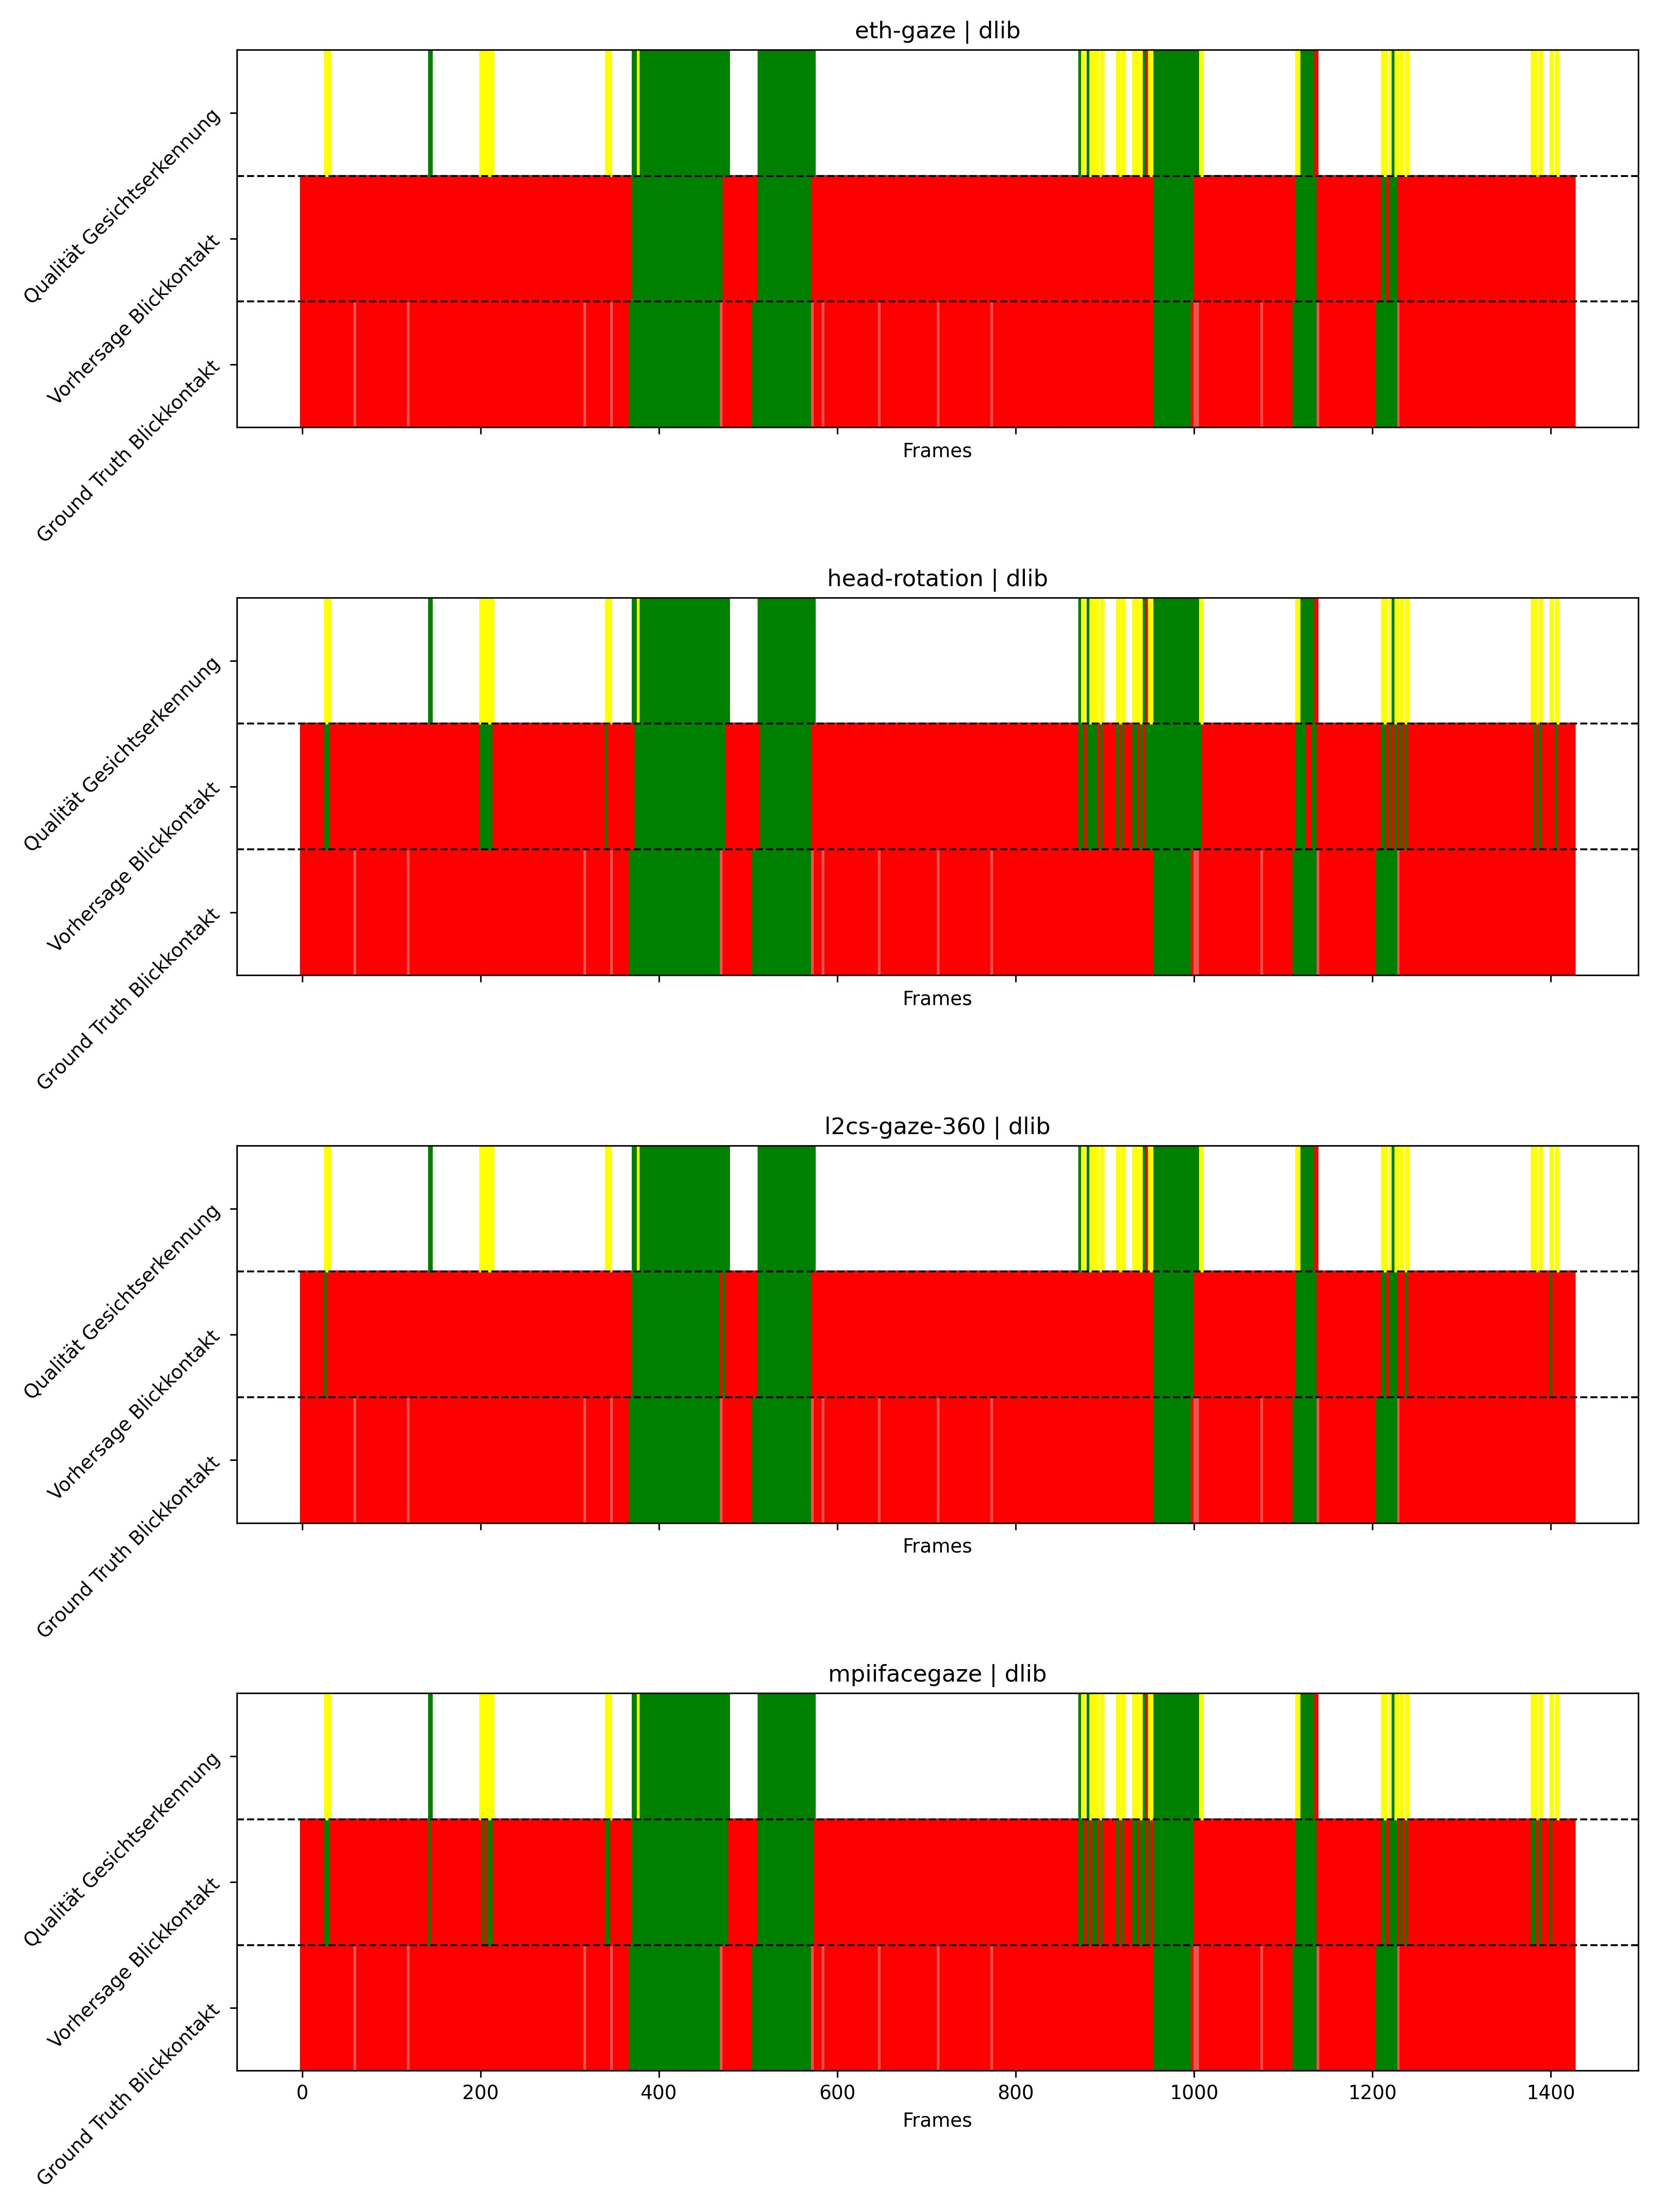
\includegraphics[width=1\linewidth]{appendix/01-dlib-overview-gaze.jpg}
\caption{Überblick über die Ground Truth des Blickkontakts, die Vorhersage des Blickkontakts und die Qualität der Gesichtserkennung mit \dlib. Die Bedeutung der Farben ist in Abbildung \ref{fig:evaluation:gaze:mpiifacegaze} erklärt.  }
\end{figure}

\begin{figure}[H]
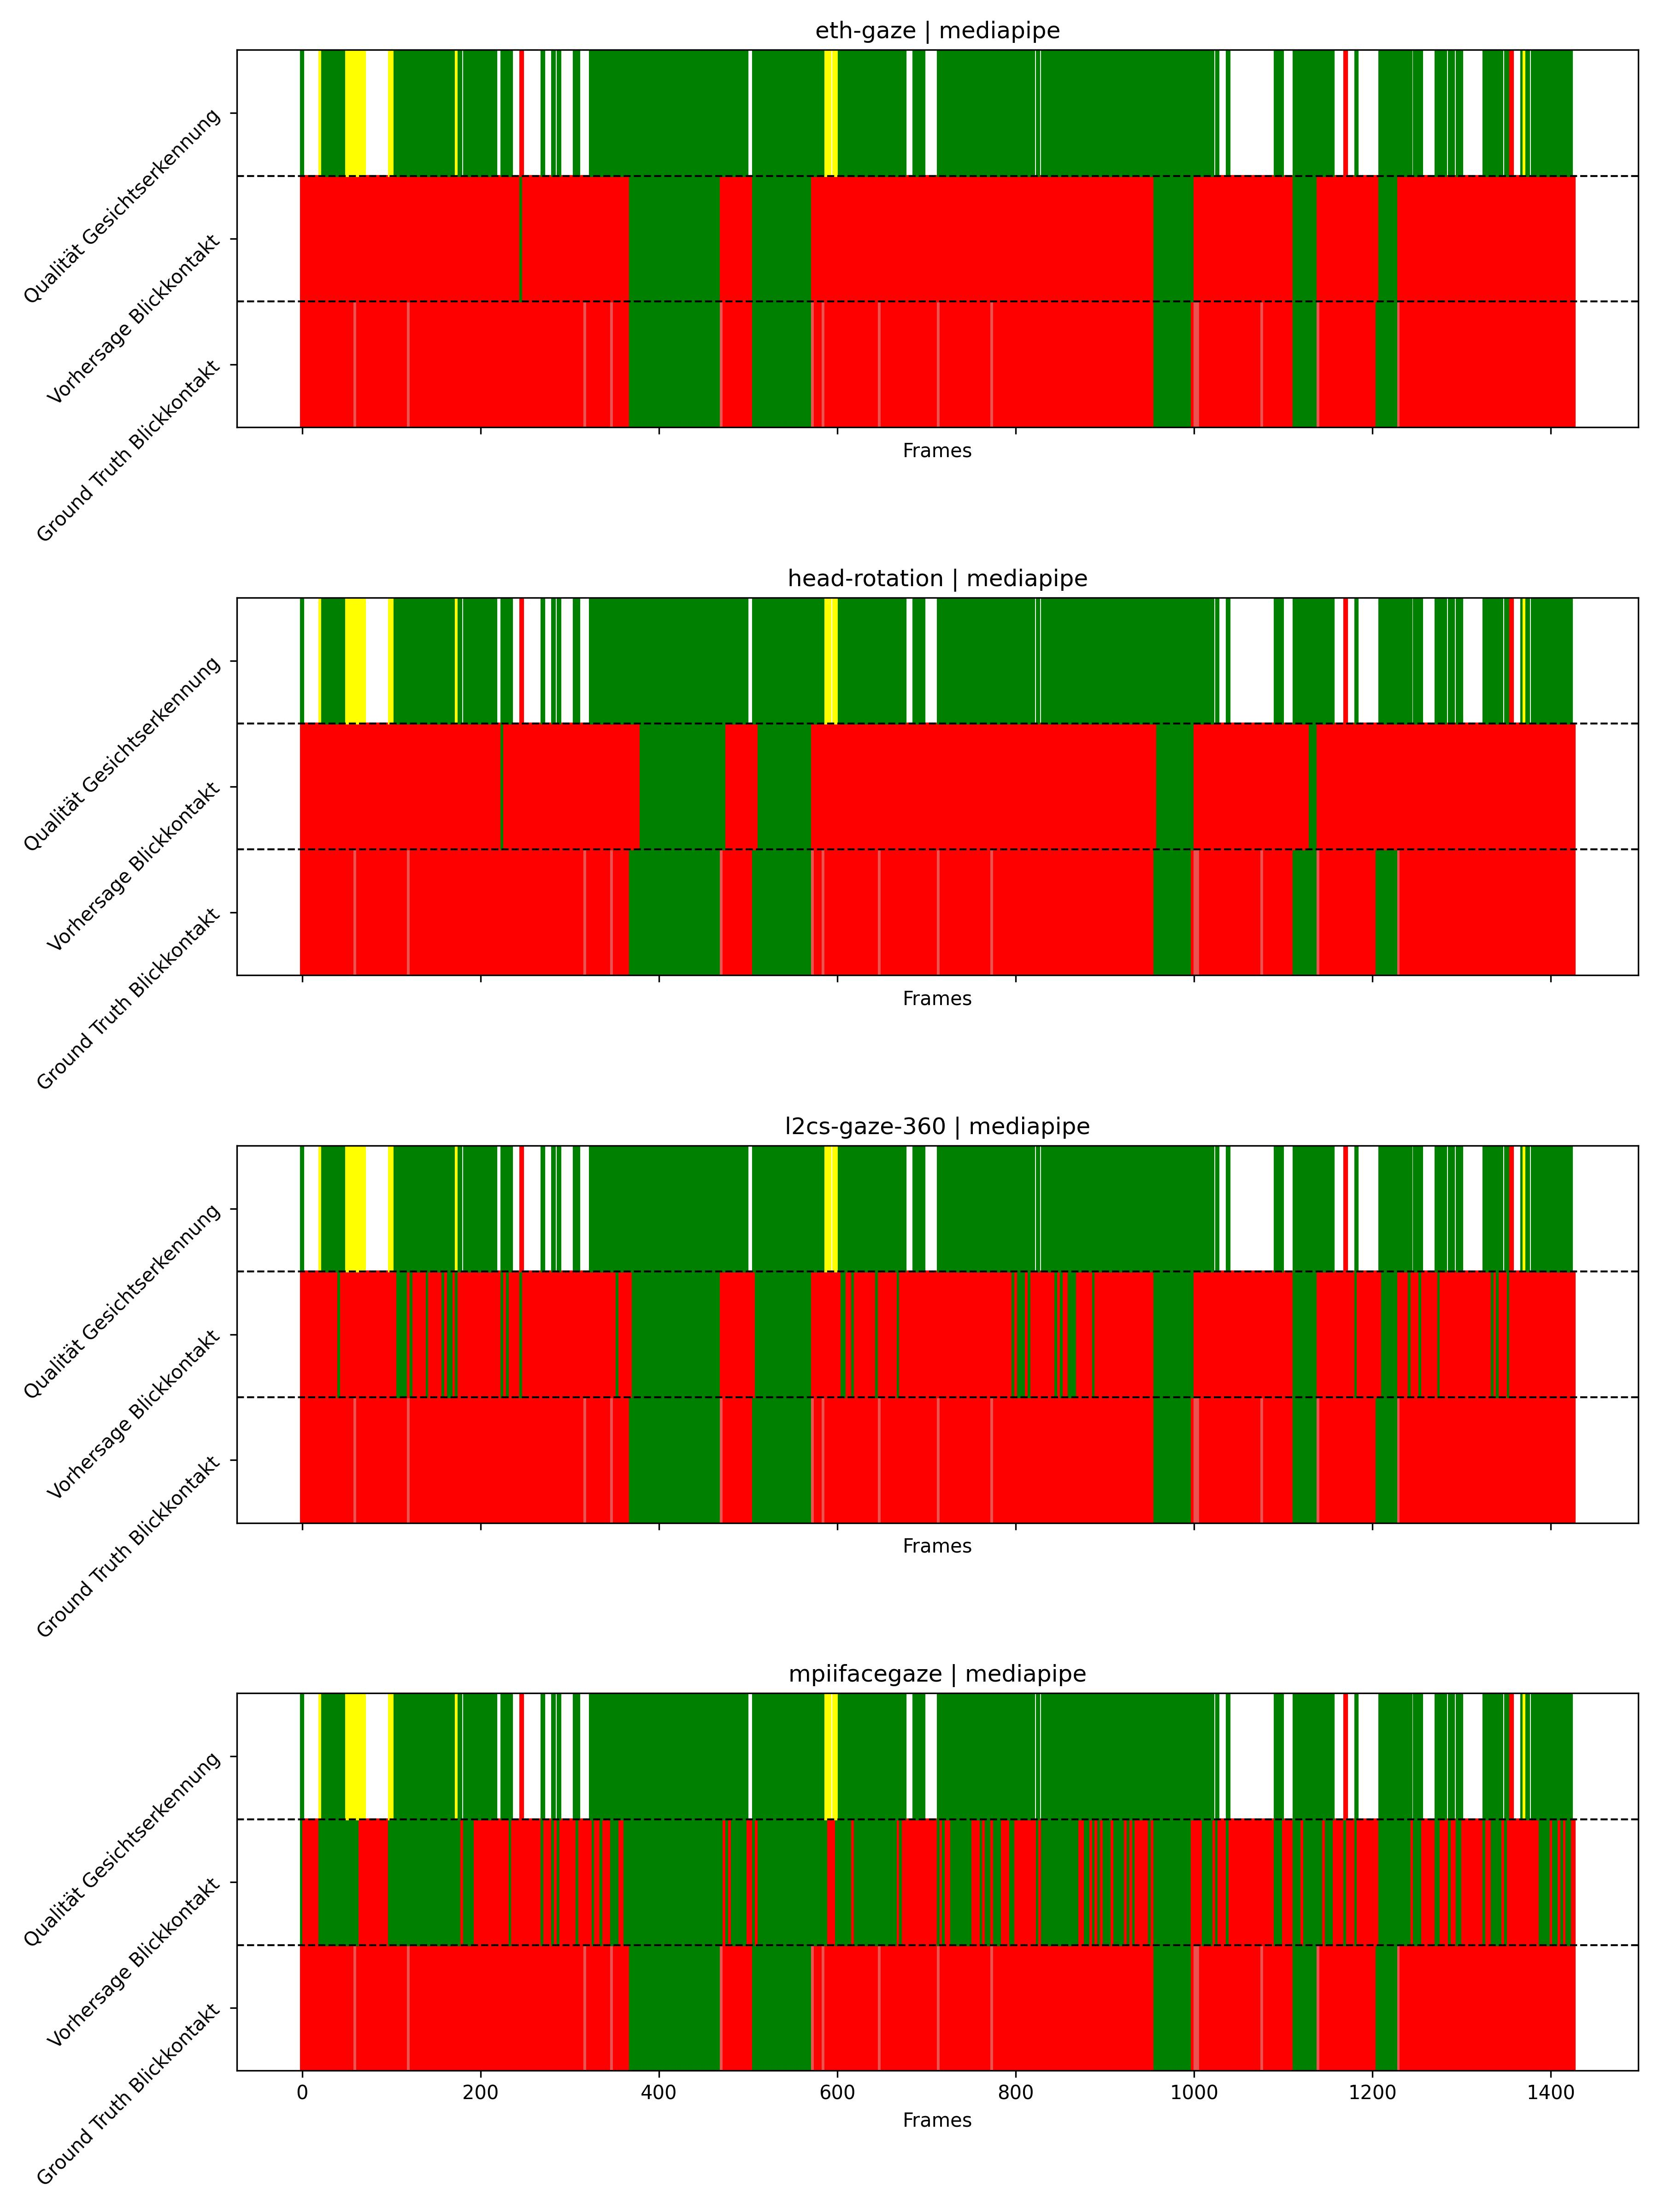
\includegraphics[width=1\linewidth]{appendix/01-mediapipe-overview-gaze.jpg}
\caption{Überblick über die Ground Truth des Blickkontakts, die Vorhersage des Blickkontakts und die Qualität der Gesichtserkennung mit \mediapipe. Die Bedeutung der Farben ist in Abbildung \ref{fig:evaluation:gaze:mpiifacegaze} erklärt.}
\end{figure}

\section{Video 02}
\begin{figure}[H]
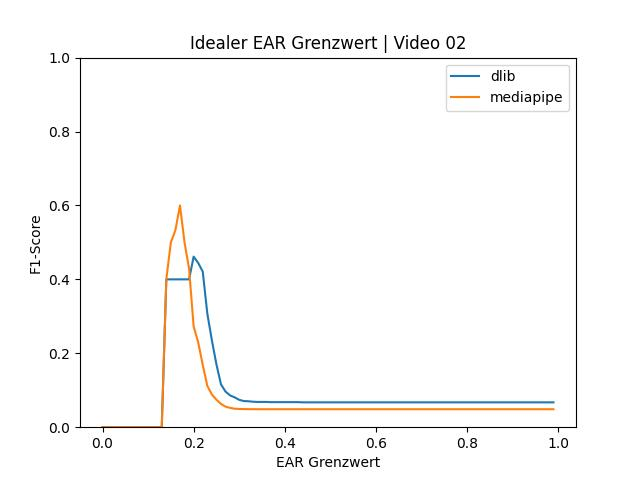
\includegraphics[width=0.7\linewidth]{appendix/02_f1-score-blink.jpg}
\caption{Ergebnisse der Bestimmung des idealen EAR-Grenzwerts für Video 02.}
\end{figure}

\begin{figure}[H]
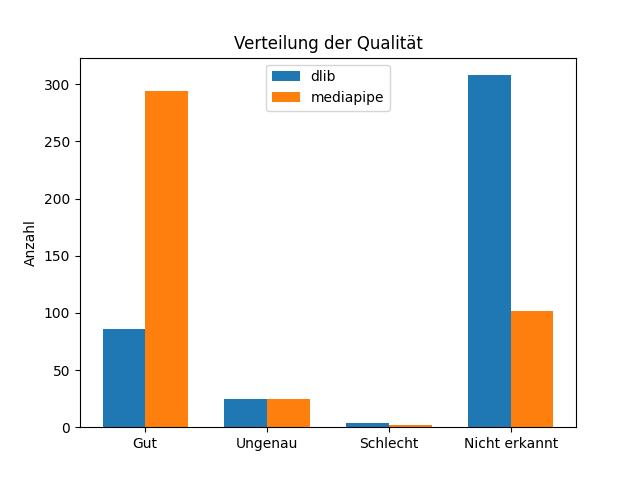
\includegraphics[width=0.7\linewidth]{appendix/02_bar-quality.jpg}
\caption{Aufteilung der Gesichtserkennungsqualität von Video 02.}
\end{figure}

\begin{table}[H]
\centering
\begin{tabular}{l|l|c c |c}
\toprule
\textbf{Gesichtserkennung} & \textbf{Blickrichtung} & \textbf{Seitenlänge} $\hitthresholdsize$ & \textbf{Verschiebung} $\hitthresholdposition$ & \textbf{F1-Score} \\ 
\midrule
\multirow{4}*{dlib}& ETH-XGaze & 0,092 & -0,014 & 0,956  \\ 
& Gaze360 & 0,286 & 0,047 & 0,906 \\ 
& MPIIFaceGaze & 0,031 & -0,027 & 0,785  \\ 
& Kopfrotation & 0,071 & 0,182 & 0,807  \\ 
\hline\multirow{4}*{MediaPipe}& ETH-XGaze & 0,092 & -0,014 & 0,974  \\ 
& Gaze360 & 0,255 & 0,047 & 0,862 \\ 
& MPIIFaceGaze & 0,031 & -0,027 & 0,591  \\ 
& Kopfrotation & 0,143 & 0,206 & 0,911  \\ 
\bottomrule\end{tabular}
\caption{Ergebnis des Hyperparameter-Tunings für die Zone speziell für Video 02.}
\label{tab:appendix:02:local}
\end{table}
\begin{table}[H]
\centering
\begin{tabular}{l|l|c c c c|c c|c}
\toprule
\textbf{Gesichtserkennung} & \textbf{Blickrichtung} & $TP$ & $TN$& $FP$ & $FN$ & \textbf{Precision} & \textbf{Recall} & \textbf{F1-Score} \\ 
\midrule
\multirow{4}*{dlib}& ETH-XGaze & 54 & 360 & 3 & 3 & 0,947 & 0,947 & 0,947 \\ 
& Gaze360 & 53 & 351 & 12 & 4 & 0,815 & 0,93 & 0,869 \\ 
& MPIIFaceGaze & 54 & 326 & 37 & 3 & 0,593 & 0,947 & 0,73 \\ 
& Kopfrotation & 52 & 329 & 34 & 5 & 0,605 & 0,912 & 0,727 \\ 
\hline\multirow{4}*{MediaPipe}& ETH-XGaze & 58 & 358 & 7 & 0 & 0,892 & 1,0 & 0,943 \\ 
& Gaze360 & 52 & 352 & 13 & 6 & 0,8 & 0,897 & 0,846 \\ 
& MPIIFaceGaze & 56 & 218 & 147 & 2 & 0,276 & 0,966 & 0,429 \\ 
& Kopfrotation & 51 & 361 & 4 & 7 & 0,927 & 0,879 & 0,903 \\ 
\bottomrule\end{tabular}
\caption{Zusammensetzung des F1-Scores unter Verwendung der in Kapitel \ref{sec:evaluation:results:gaze:threshold} bestimmten globalen Parameter $\hitthresholdsize$ und $\hitthresholdposition$.}
\label{tab:appendix:02:f1}
\end{table}
\begin{figure}[H]
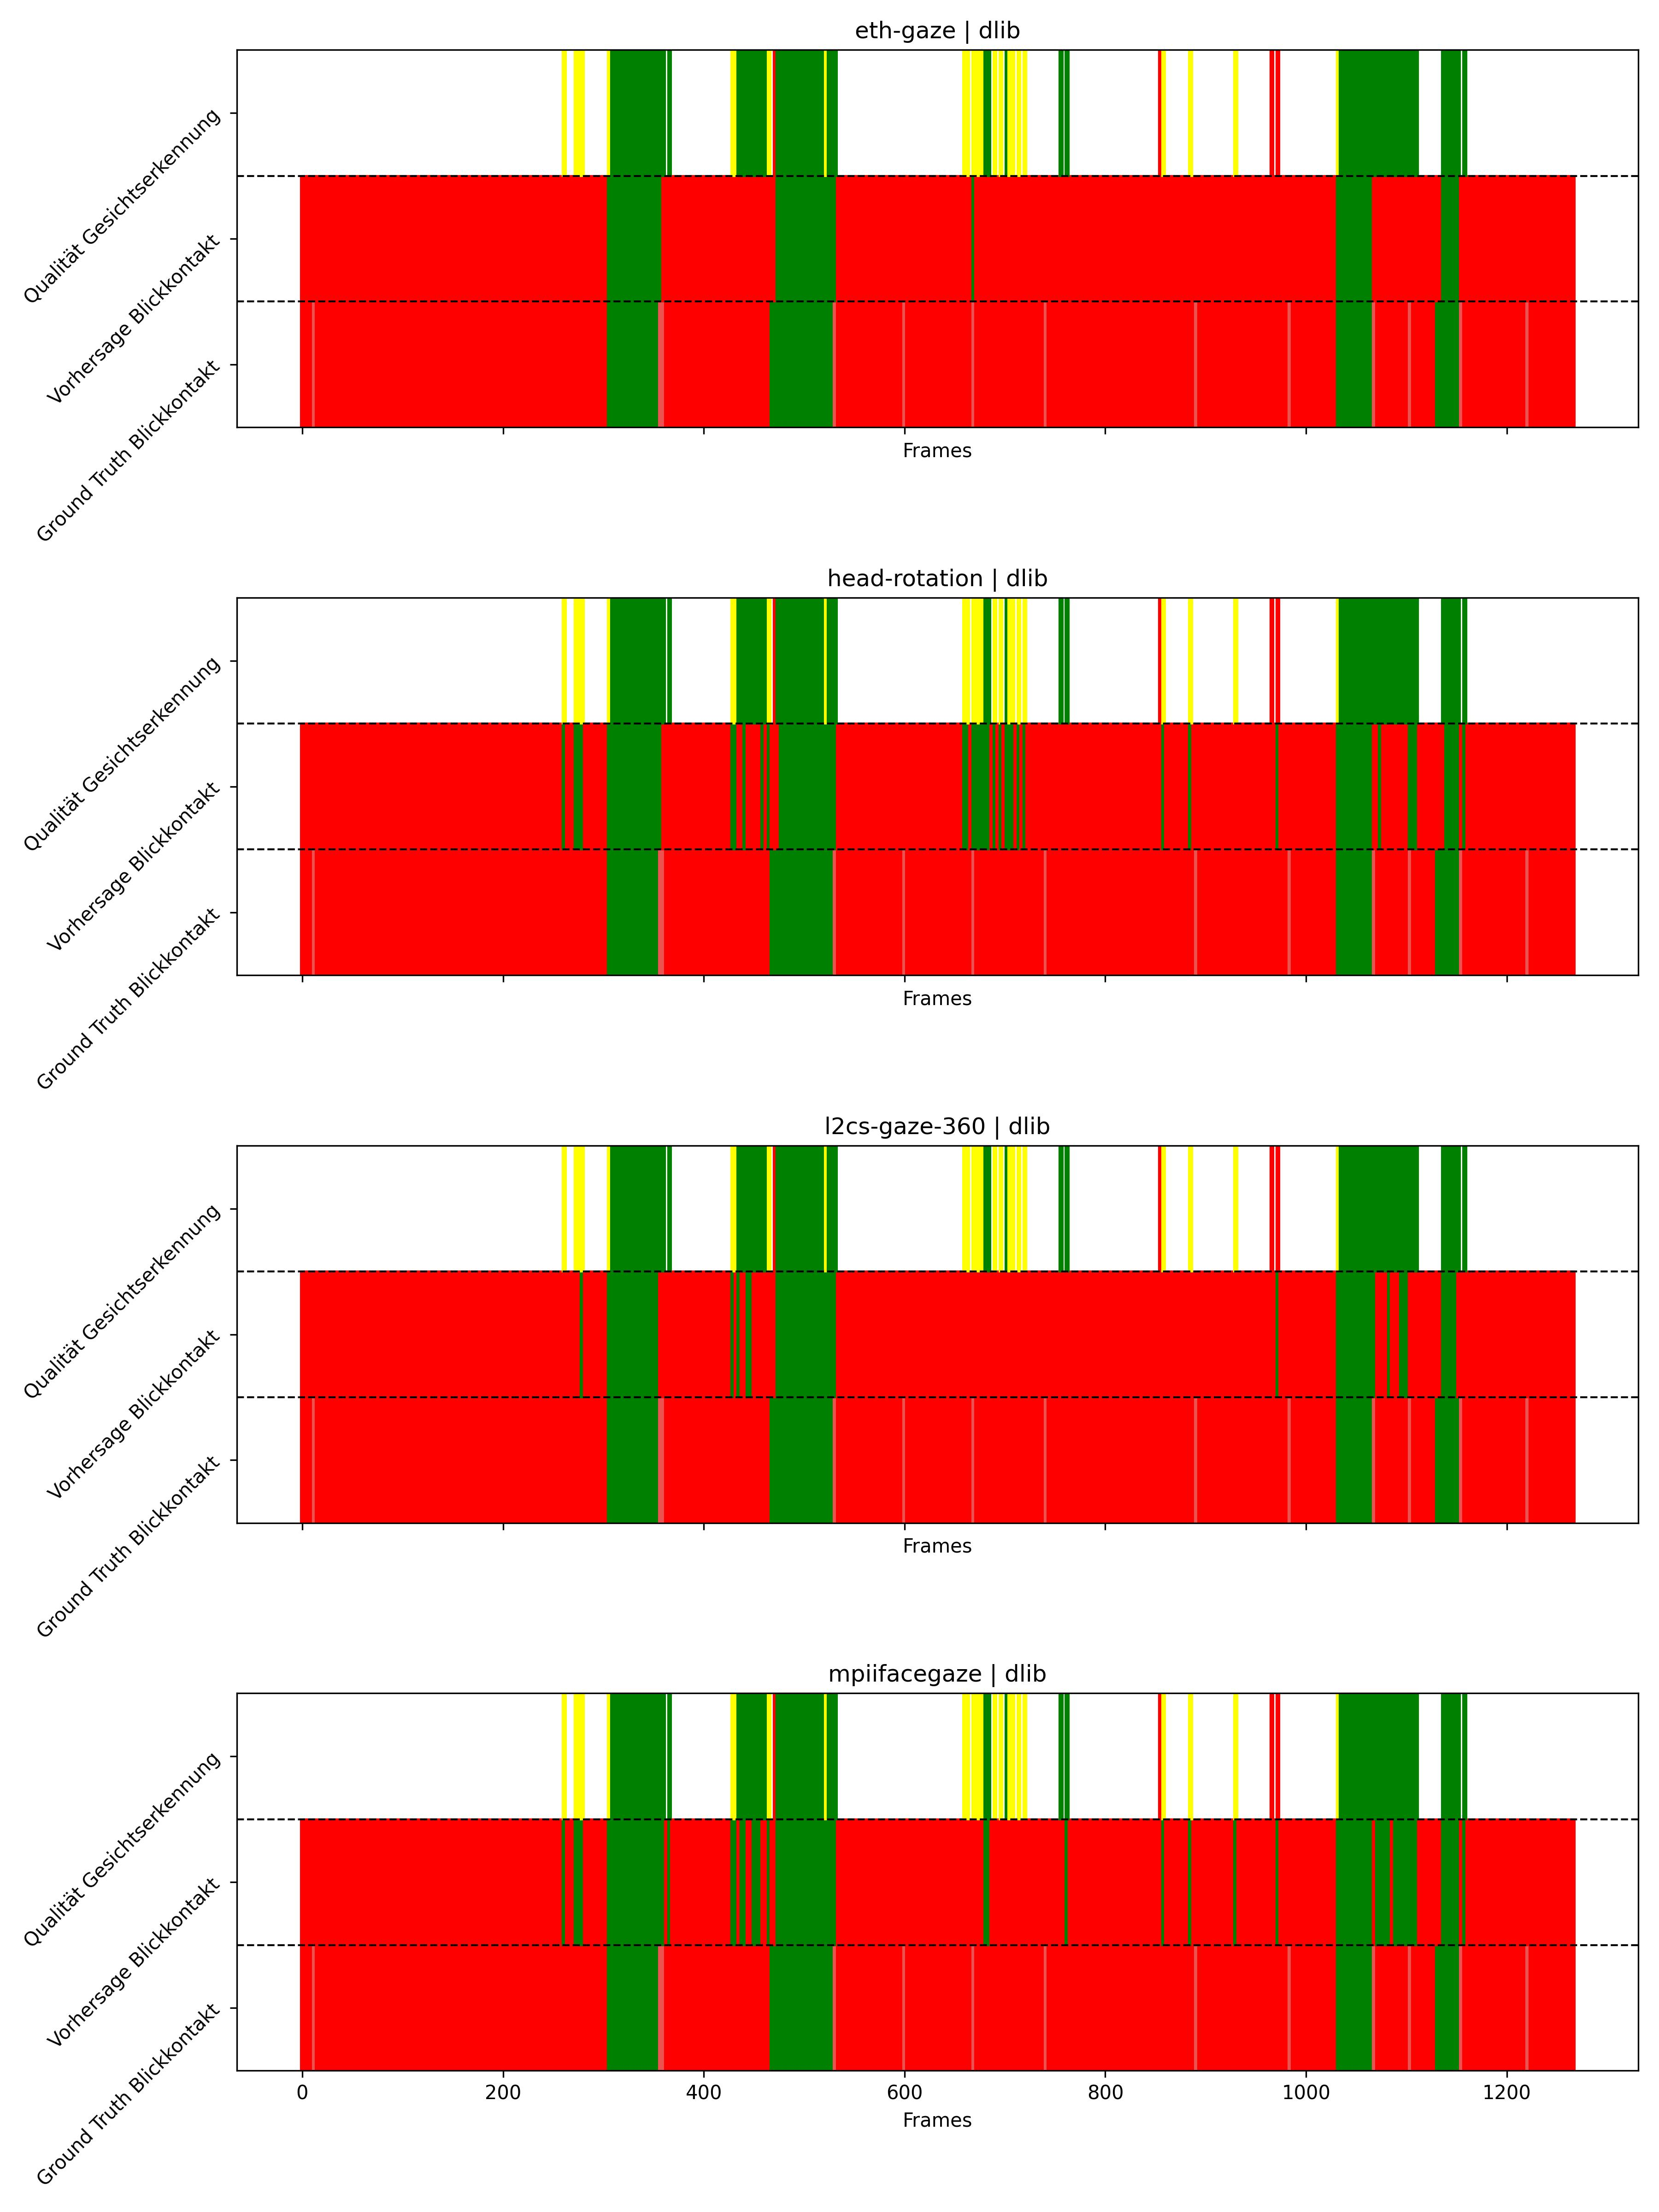
\includegraphics[width=1\linewidth]{appendix/02-dlib-overview-gaze.jpg}
\caption{Überblick über die Ground Truth des Blickkontakts, die Vorhersage des Blickkontakts und die Qualität der Gesichtserkennung mit \dlib. Die Bedeutung der Farben ist in Abbildung \ref{fig:evaluation:gaze:mpiifacegaze} erklärt.  }
\end{figure}

\begin{figure}[H]
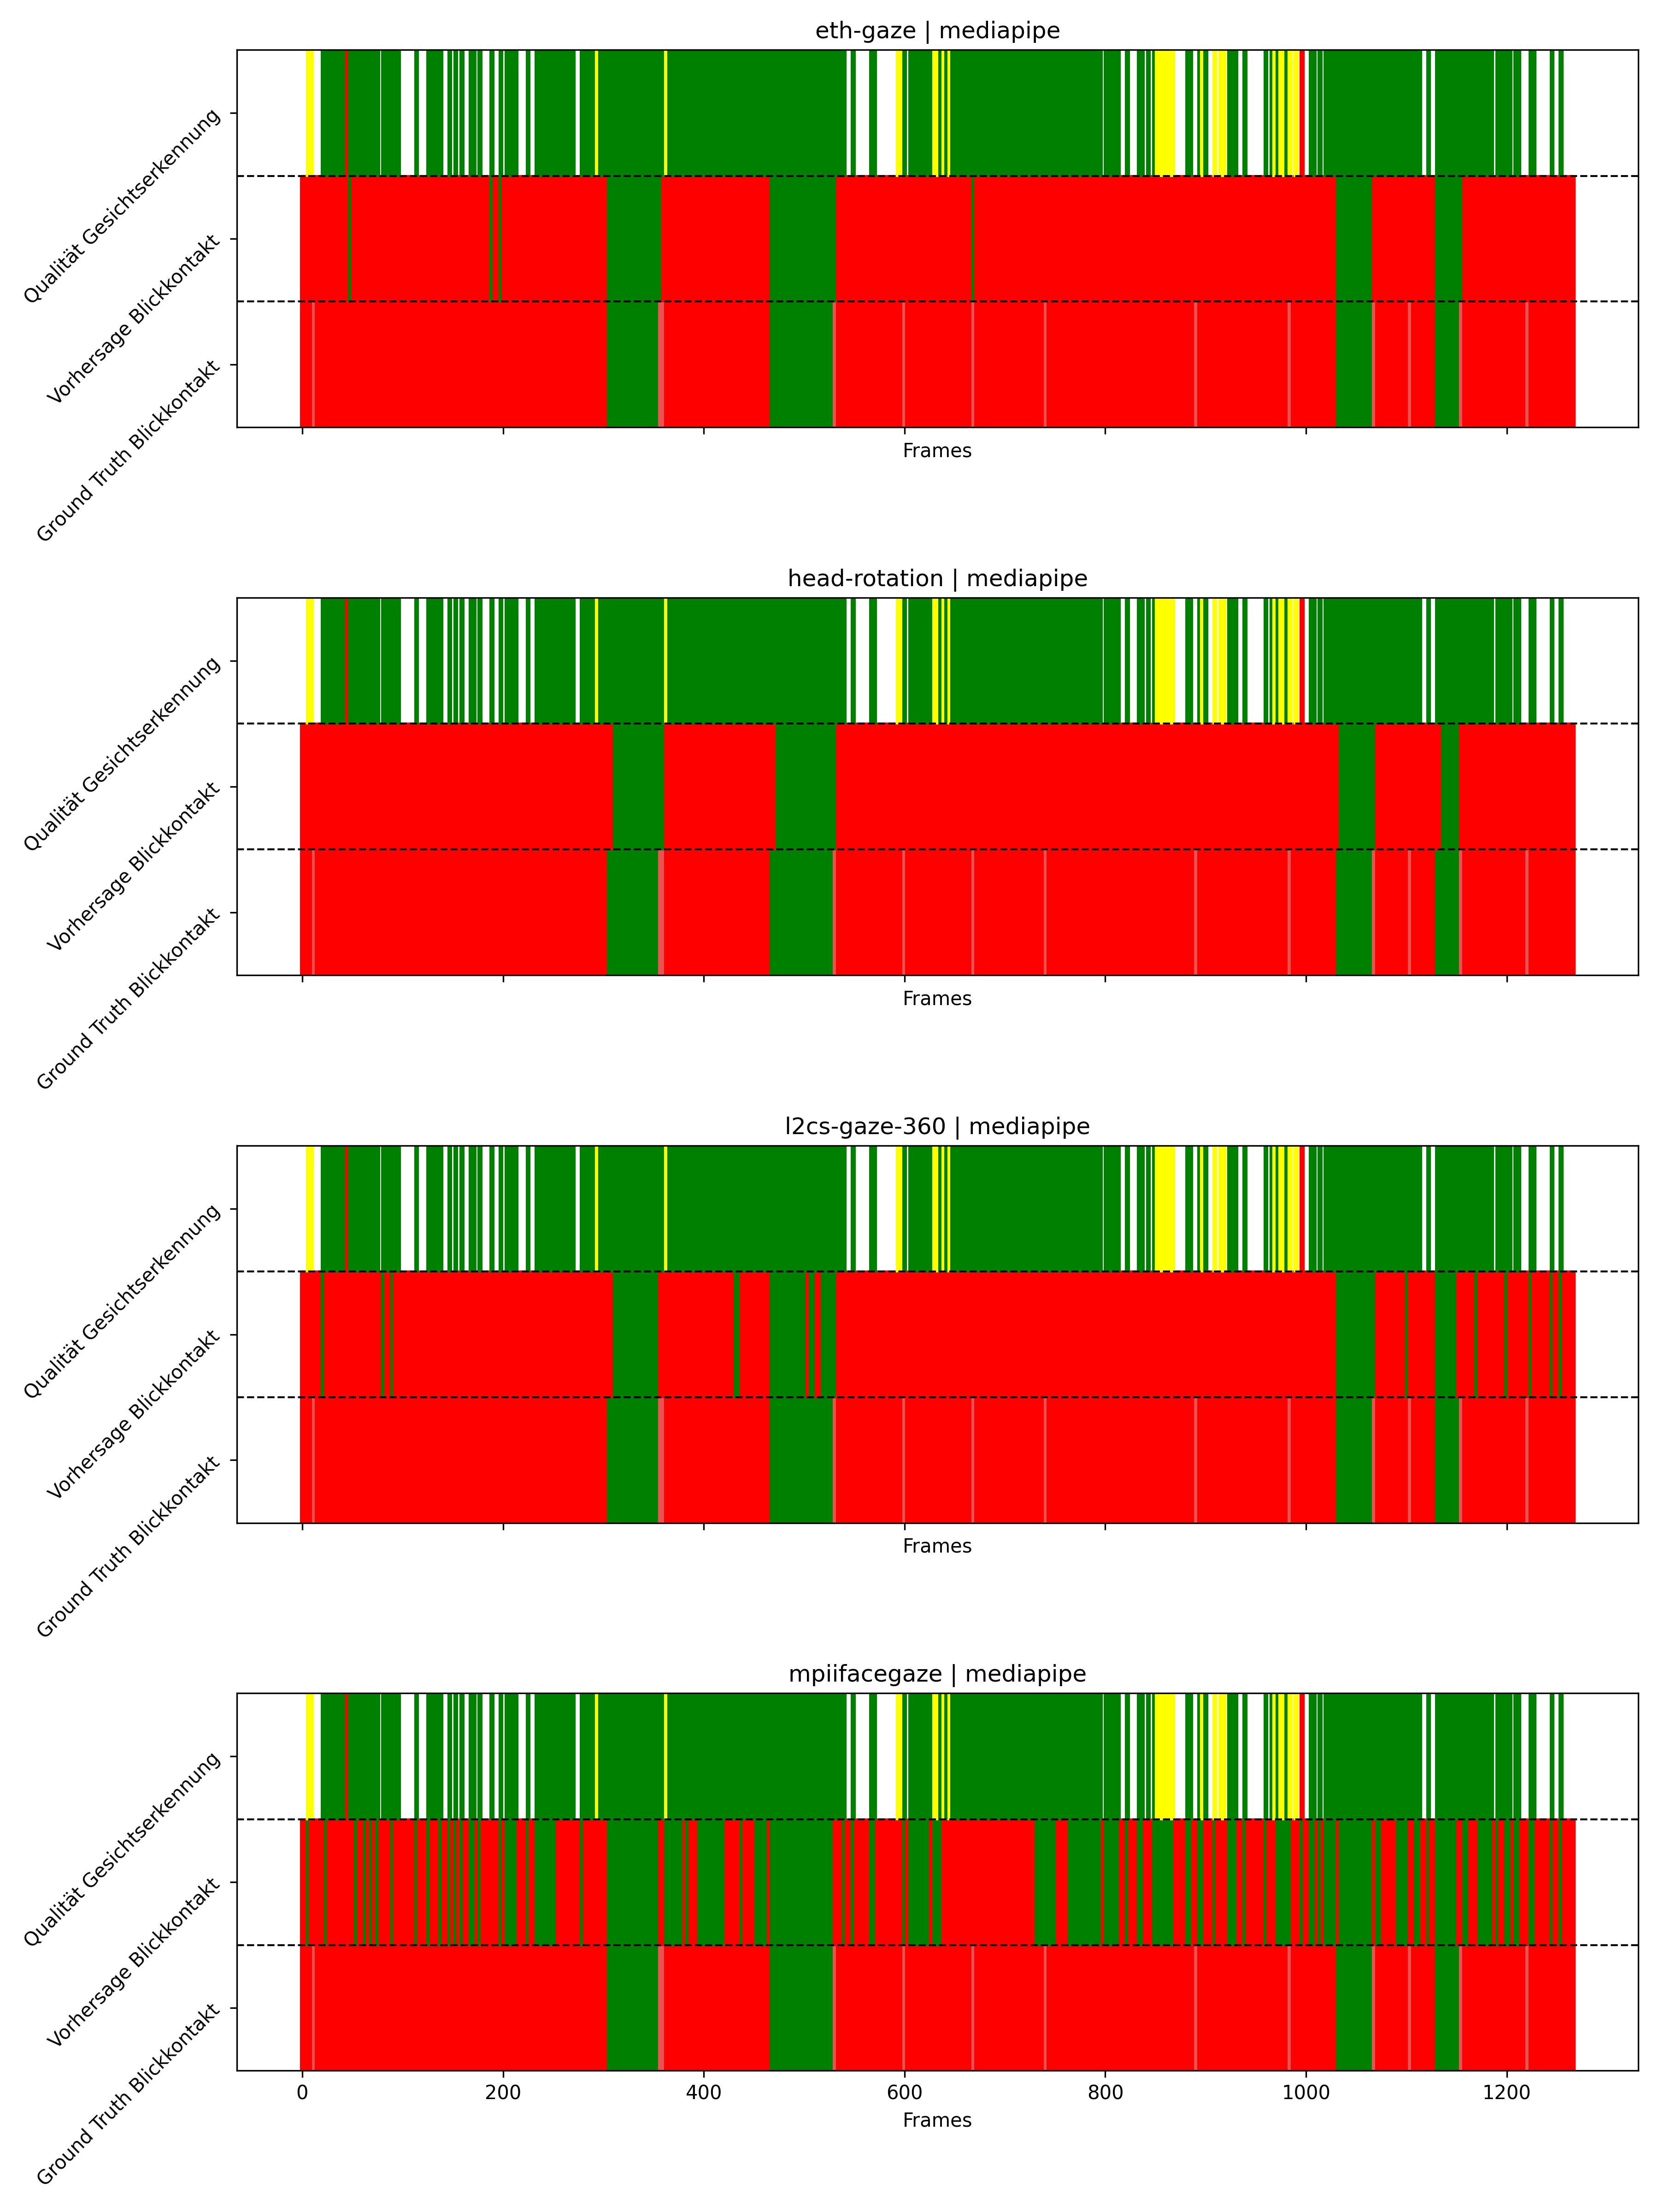
\includegraphics[width=1\linewidth]{appendix/02-mediapipe-overview-gaze.jpg}
\caption{Überblick über die Ground Truth des Blickkontakts, die Vorhersage des Blickkontakts und die Qualität der Gesichtserkennung mit \mediapipe. Die Bedeutung der Farben ist in Abbildung \ref{fig:evaluation:gaze:mpiifacegaze} erklärt.}
\end{figure}

\section{Video 03}
\begin{figure}[H]
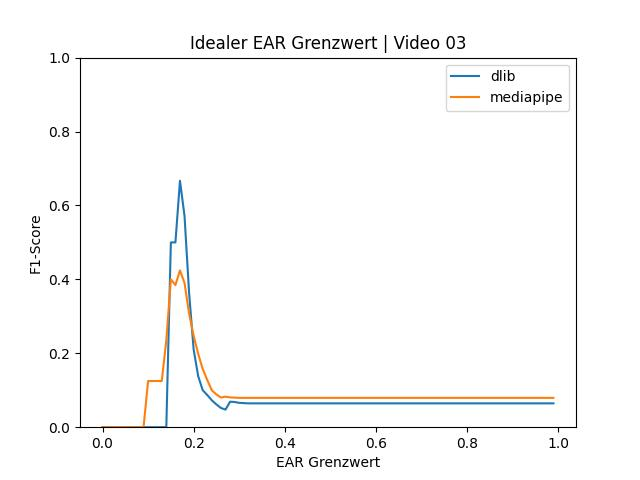
\includegraphics[width=0.7\linewidth]{appendix/03_f1-score-blink.jpg}
\caption{Ergebnisse der Bestimmung des idealen EAR-Grenzwerts für Video 03.}
\end{figure}

\begin{figure}[H]
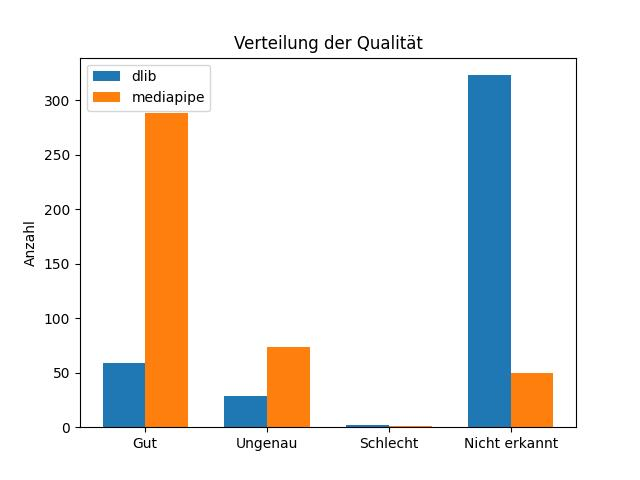
\includegraphics[width=0.7\linewidth]{appendix/03_bar-quality.jpg}
\caption{Aufteilung der Gesichtserkennungsqualität von Video 03.}
\end{figure}

\begin{table}[H]
\centering
\begin{tabular}{l|l|c c |c}
\toprule
\textbf{Gesichtserkennung} & \textbf{Blickrichtung} & \textbf{Seitenlänge} $\hitthresholdsize$ & \textbf{Verschiebung} $\hitthresholdposition$ & \textbf{F1-Score} \\ 
\midrule
\multirow{4}*{dlib}& ETH-XGaze & 0,061 & -0,039 & 0,972  \\ 
& Gaze360 & 0,214 & 0,035 & 0,907 \\ 
& MPIIFaceGaze & 0,02 & -0,039 & 0,683  \\ 
& Kopfrotation & 0,102 & 0,194 & 0,895  \\ 
\hline\multirow{4}*{MediaPipe}& ETH-XGaze & 0,092 & -0,014 & 0,986  \\ 
& Gaze360 & 0,214 & 0,035 & 0,695 \\ 
& MPIIFaceGaze & 0,02 & -0,039 & 0,525  \\ 
& Kopfrotation & 0,112 & 0,206 & 0,971  \\ 
\bottomrule\end{tabular}
\caption{Ergebnis des Hyperparameter-Tunings für die Zone speziell für Video 03.}
\label{tab:appendix:03:local}
\end{table}
\begin{table}[H]
\centering
\begin{tabular}{l|l|c c c c|c c|c}
\toprule
\textbf{Gesichtserkennung} & \textbf{Blickrichtung} & $TP$ & $TN$& $FP$ & $FN$ & \textbf{Precision} & \textbf{Recall} & \textbf{F1-Score} \\ 
\midrule
\multirow{4}*{dlib}& ETH-XGaze & 35 & 375 & 2 & 1 & 0,946 & 0,972 & 0,959 \\ 
& Gaze360 & 35 & 365 & 12 & 1 & 0,745 & 0,972 & 0,843 \\ 
& MPIIFaceGaze & 35 & 328 & 49 & 1 & 0,417 & 0,972 & 0,583 \\ 
& Kopfrotation & 34 & 352 & 25 & 2 & 0,576 & 0,944 & 0,716 \\ 
\hline\multirow{4}*{MediaPipe}& ETH-XGaze & 36 & 375 & 2 & 0 & 0,947 & 1,0 & 0,973 \\ 
& Gaze360 & 36 & 319 & 58 & 0 & 0,383 & 1,0 & 0,554 \\ 
& MPIIFaceGaze & 36 & 132 & 245 & 0 & 0,128 & 1,0 & 0,227 \\ 
& Kopfrotation & 34 & 375 & 2 & 2 & 0,944 & 0,944 & 0,944 \\ 
\bottomrule\end{tabular}
\caption{Zusammensetzung des F1-Scores unter Verwendung der in Kapitel \ref{sec:evaluation:results:gaze:threshold} bestimmten globalen Parameter $\hitthresholdsize$ und $\hitthresholdposition$.}
\label{tab:appendix:03:f1}
\end{table}
\begin{figure}[H]
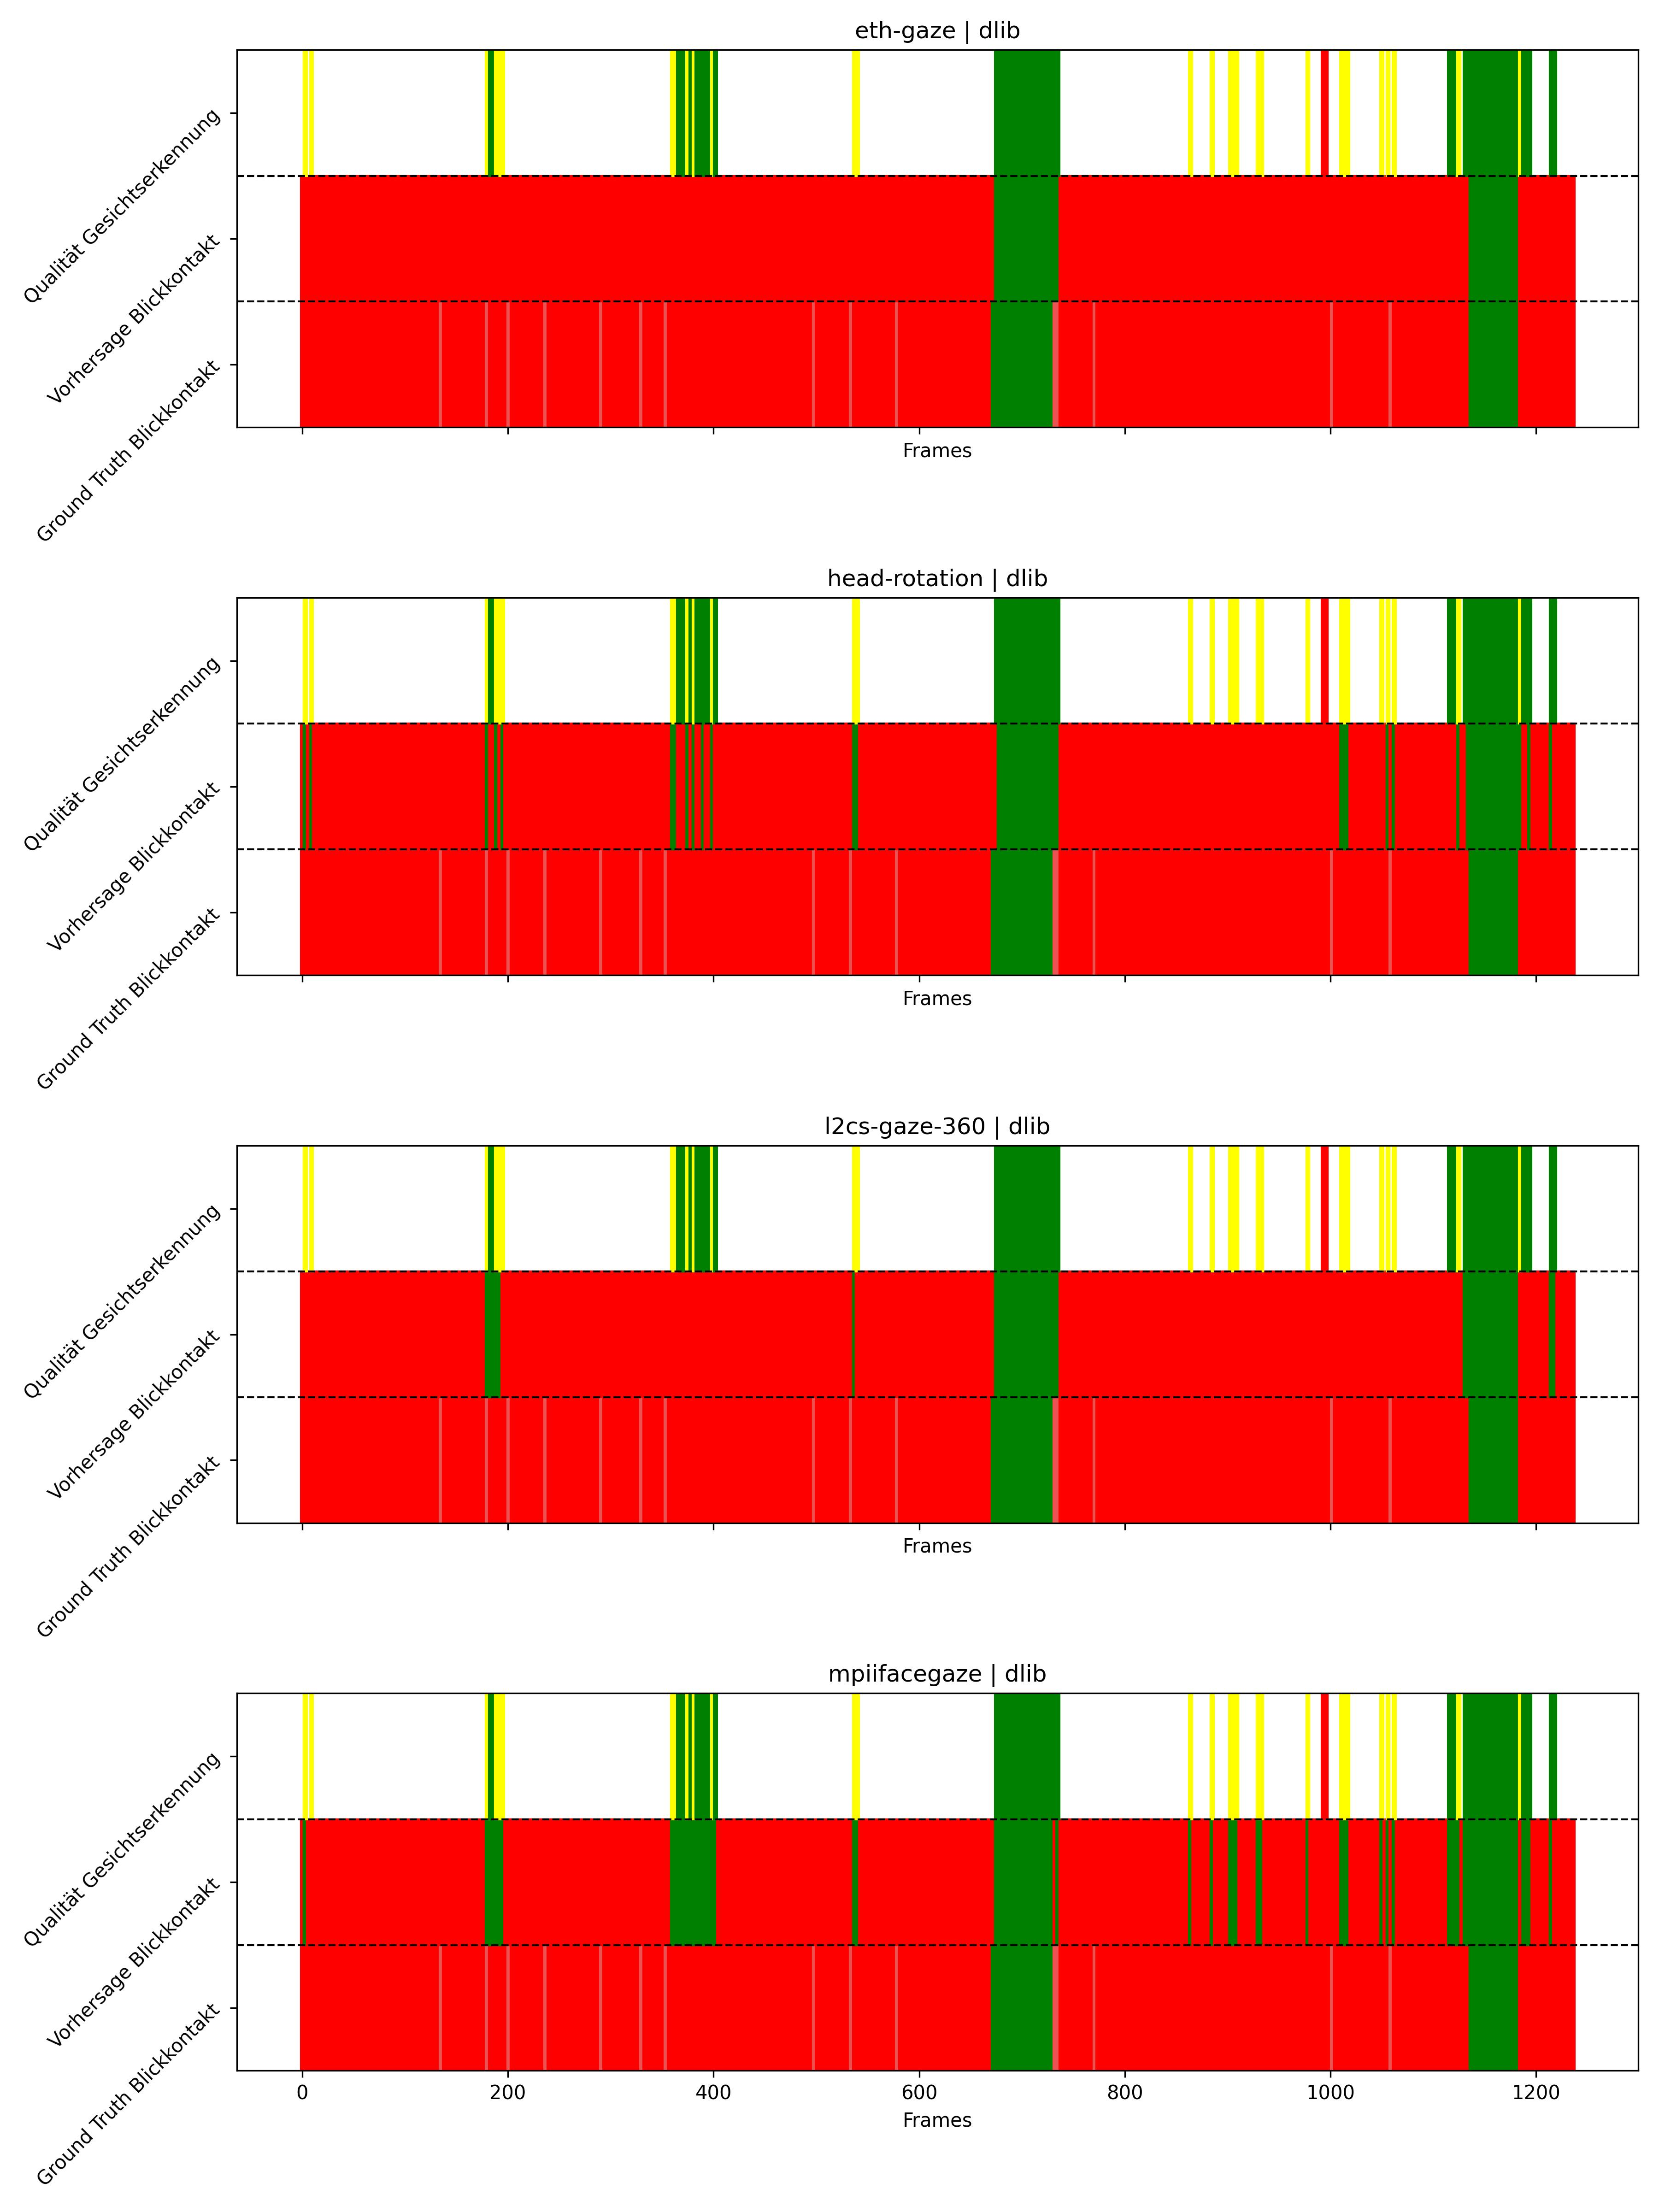
\includegraphics[width=1\linewidth]{appendix/03-dlib-overview-gaze.jpg}
\caption{Überblick über die Ground Truth des Blickkontakts, die Vorhersage des Blickkontakts und die Qualität der Gesichtserkennung mit \dlib. Die Bedeutung der Farben ist in Abbildung \ref{fig:evaluation:gaze:mpiifacegaze} erklärt.  }
\end{figure}

\begin{figure}[H]
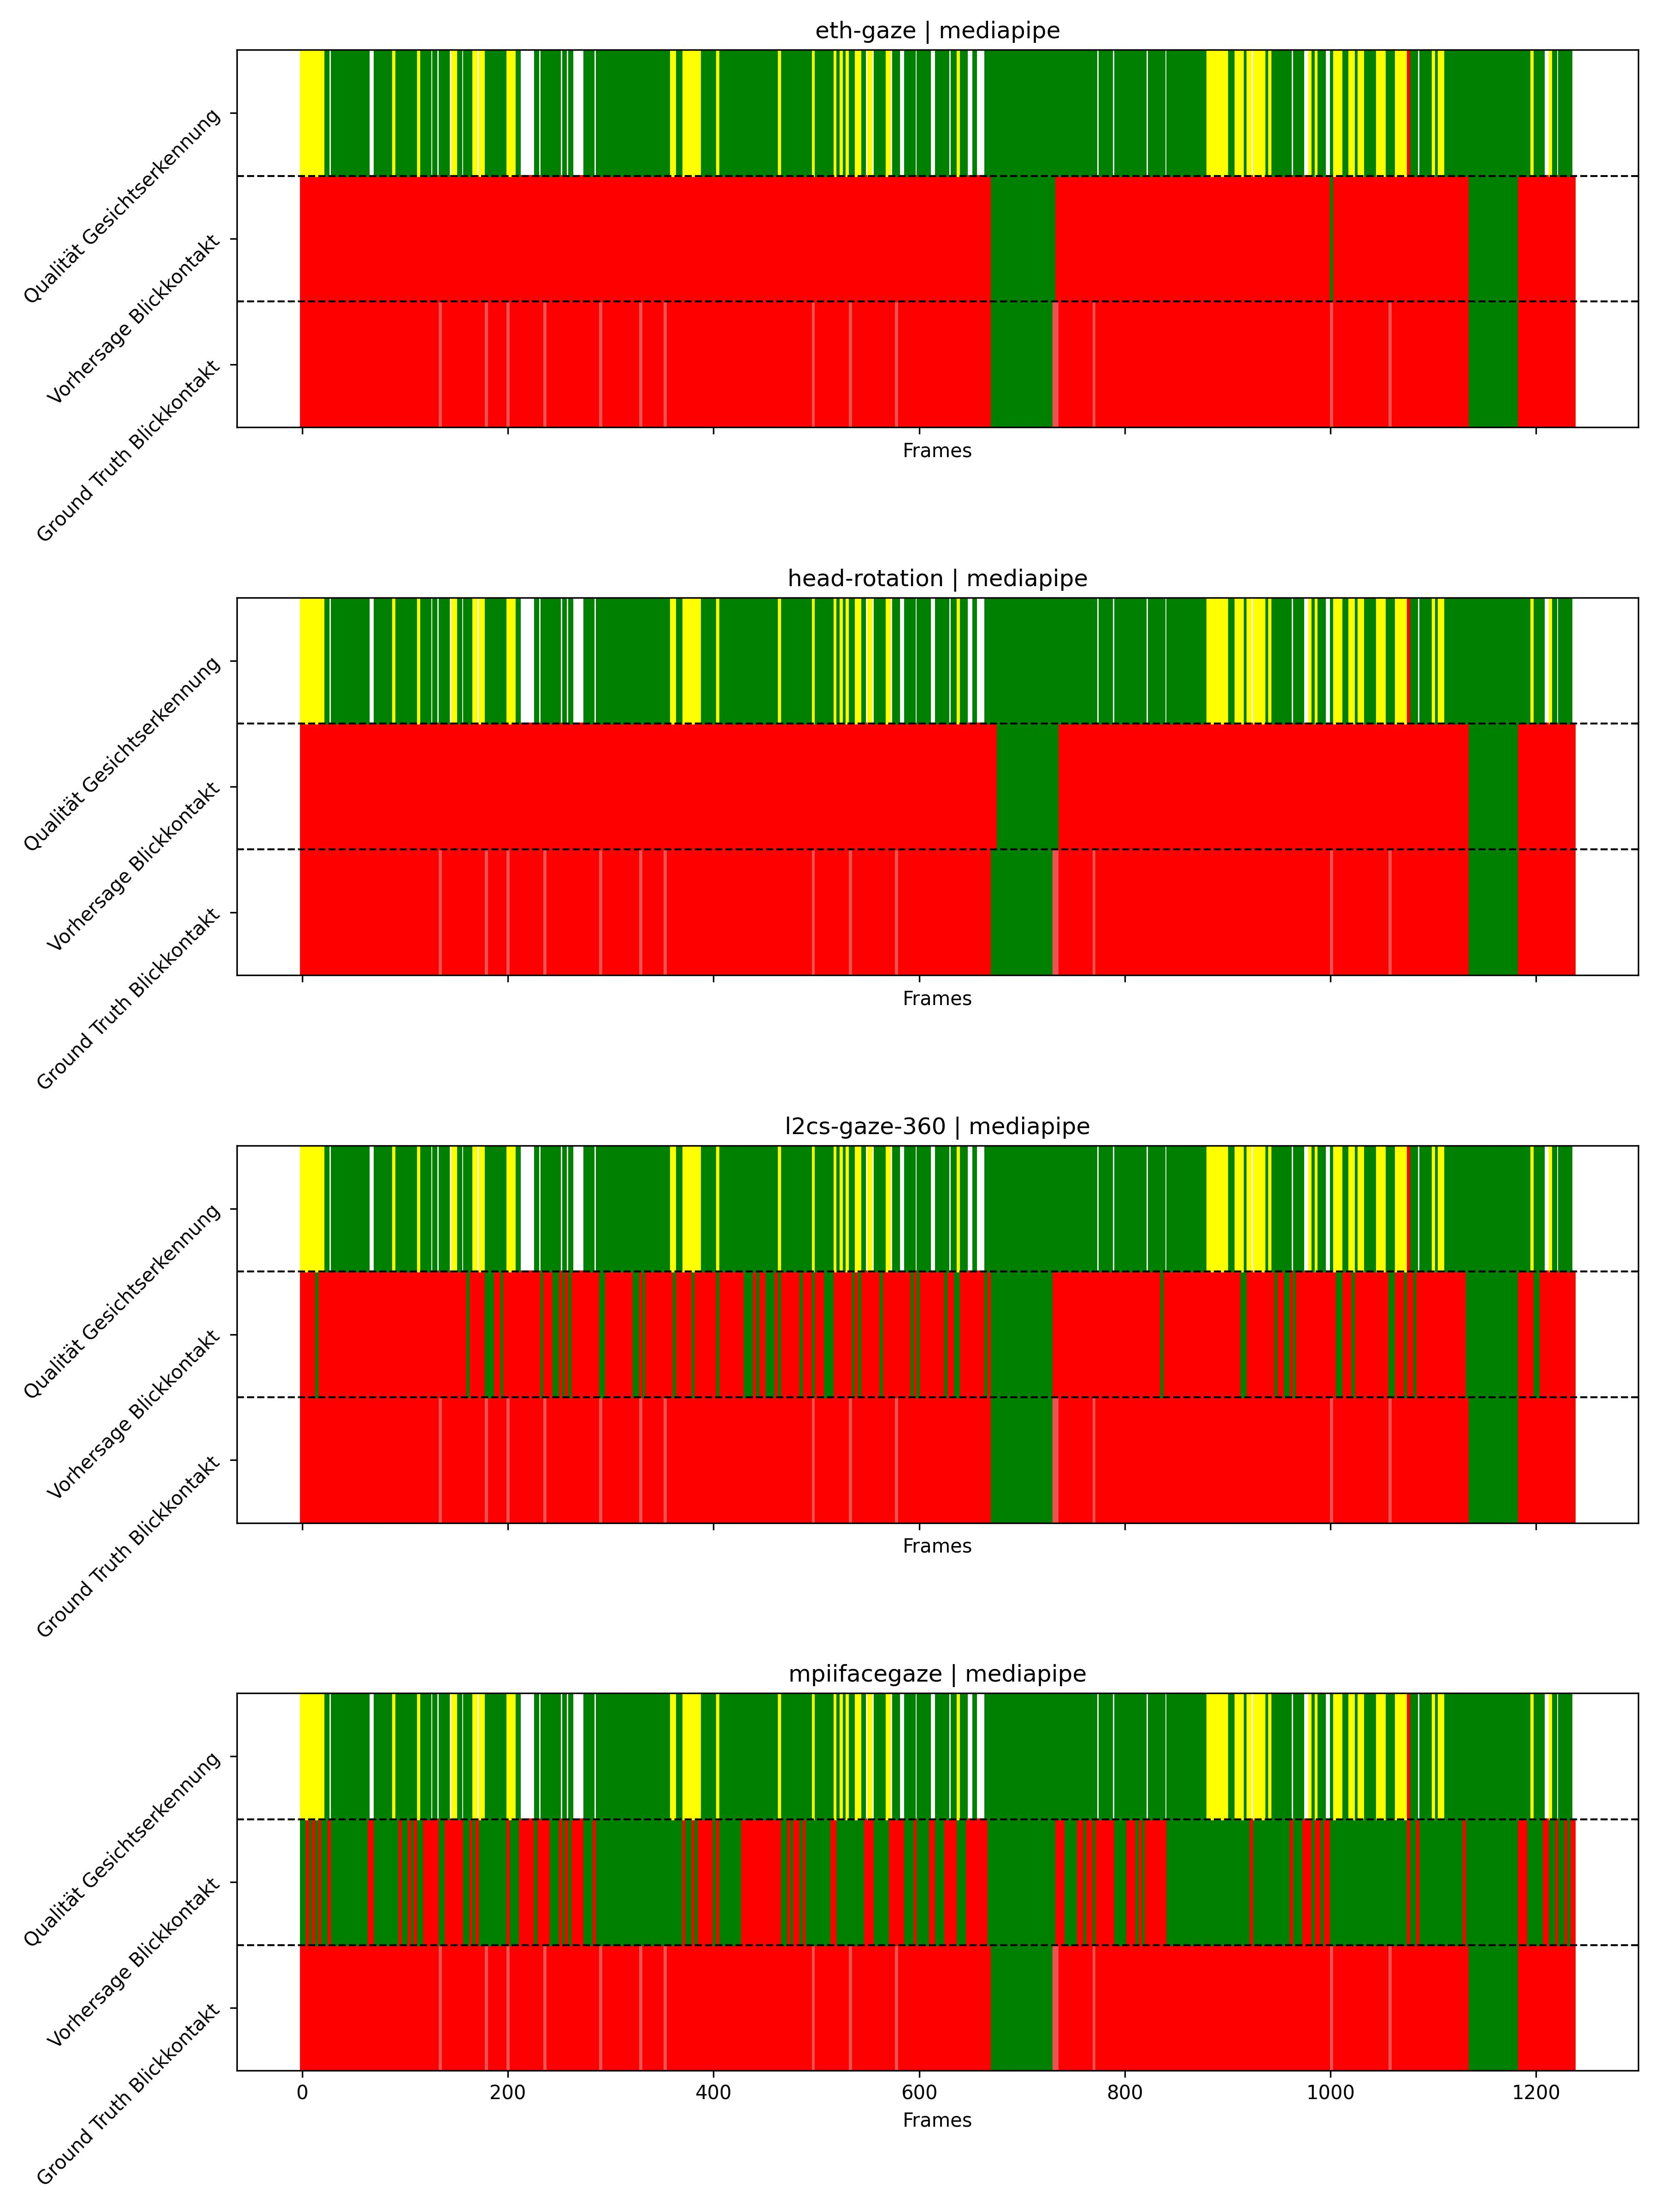
\includegraphics[width=1\linewidth]{appendix/03-mediapipe-overview-gaze.jpg}
\caption{Überblick über die Ground Truth des Blickkontakts, die Vorhersage des Blickkontakts und die Qualität der Gesichtserkennung mit \mediapipe. Die Bedeutung der Farben ist in Abbildung \ref{fig:evaluation:gaze:mpiifacegaze} erklärt.}
\end{figure}

\section{Video 04}
\begin{figure}[H]
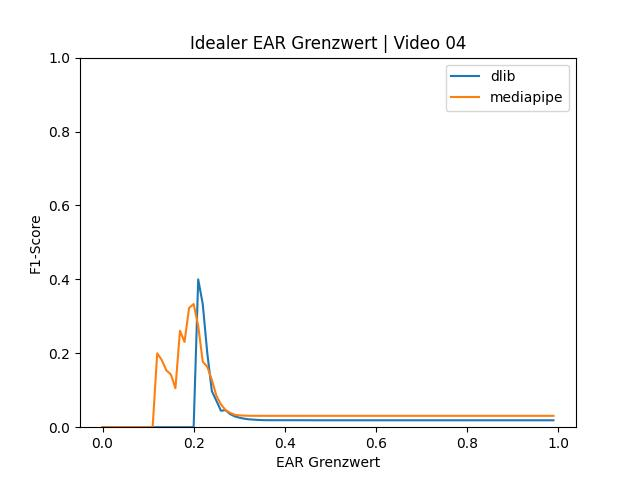
\includegraphics[width=0.7\linewidth]{appendix/04_f1-score-blink.jpg}
\caption{Ergebnisse der Bestimmung des idealen EAR-Grenzwerts für Video 04.}
\end{figure}

\begin{figure}[H]
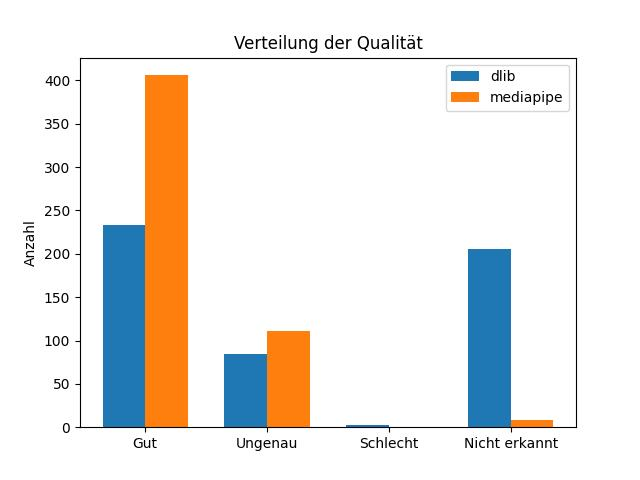
\includegraphics[width=0.7\linewidth]{appendix/04_bar-quality.jpg}
\caption{Aufteilung der Gesichtserkennungsqualität von Video 04.}
\end{figure}

\begin{table}[H]
\centering
\begin{tabular}{l|l|c c |c}
\toprule
\textbf{Gesichtserkennung} & \textbf{Blickrichtung} & \textbf{Seitenlänge} $\hitthresholdsize$ & \textbf{Verschiebung} $\hitthresholdposition$ & \textbf{F1-Score} \\ 
\midrule
\multirow{4}*{dlib}& ETH-XGaze & 0,112 & -0,014 & 0,986  \\ 
& Gaze360 & 0,316 & 0,022 & 0,904 \\ 
& MPIIFaceGaze & 0,041 & -0,027 & 0,536  \\ 
& Kopfrotation & 0,051 & 0,157 & 0,733  \\ 
\hline\multirow{4}*{MediaPipe}& ETH-XGaze & 0,122 & -0,039 & 0,993  \\ 
& Gaze360 & 0,306 & 0,035 & 0,843 \\ 
& MPIIFaceGaze & 0,031 & -0,039 & 0,474  \\ 
& Kopfrotation & 0,082 & 0,157 & 0,853  \\ 
\bottomrule\end{tabular}
\caption{Ergebnis des Hyperparameter-Tunings für die Zone speziell für Video 04.}
\label{tab:appendix:04:local}
\end{table}
\begin{table}[H]
\centering
\begin{tabular}{l|l|c c c c|c c|c}
\toprule
\textbf{Gesichtserkennung} & \textbf{Blickrichtung} & $TP$ & $TN$& $FP$ & $FN$ & \textbf{Precision} & \textbf{Recall} & \textbf{F1-Score} \\ 
\midrule
\multirow{4}*{dlib}& ETH-XGaze & 68 & 449 & 8 & 0 & 0,895 & 1,0 & 0,944 \\ 
& Gaze360 & 67 & 417 & 40 & 1 & 0,626 & 0,985 & 0,766 \\ 
& MPIIFaceGaze & 64 & 342 & 115 & 4 & 0,358 & 0,941 & 0,518 \\ 
& Kopfrotation & 65 & 295 & 162 & 3 & 0,286 & 0,956 & 0,441 \\ 
\hline\multirow{4}*{MediaPipe}& ETH-XGaze & 68 & 448 & 9 & 0 & 0,883 & 1,0 & 0,938 \\ 
& Gaze360 & 67 & 424 & 33 & 1 & 0,67 & 0,985 & 0,798 \\ 
& MPIIFaceGaze & 66 & 265 & 192 & 2 & 0,256 & 0,971 & 0,405 \\ 
& Kopfrotation & 67 & 359 & 98 & 1 & 0,406 & 0,985 & 0,575 \\ 
\bottomrule\end{tabular}
\caption{Zusammensetzung des F1-Scores unter Verwendung der in Kapitel \ref{sec:evaluation:results:gaze:threshold} bestimmten globalen Parameter $\hitthresholdsize$ und $\hitthresholdposition$.}
\label{tab:appendix:04:f1}
\end{table}
\begin{figure}[H]
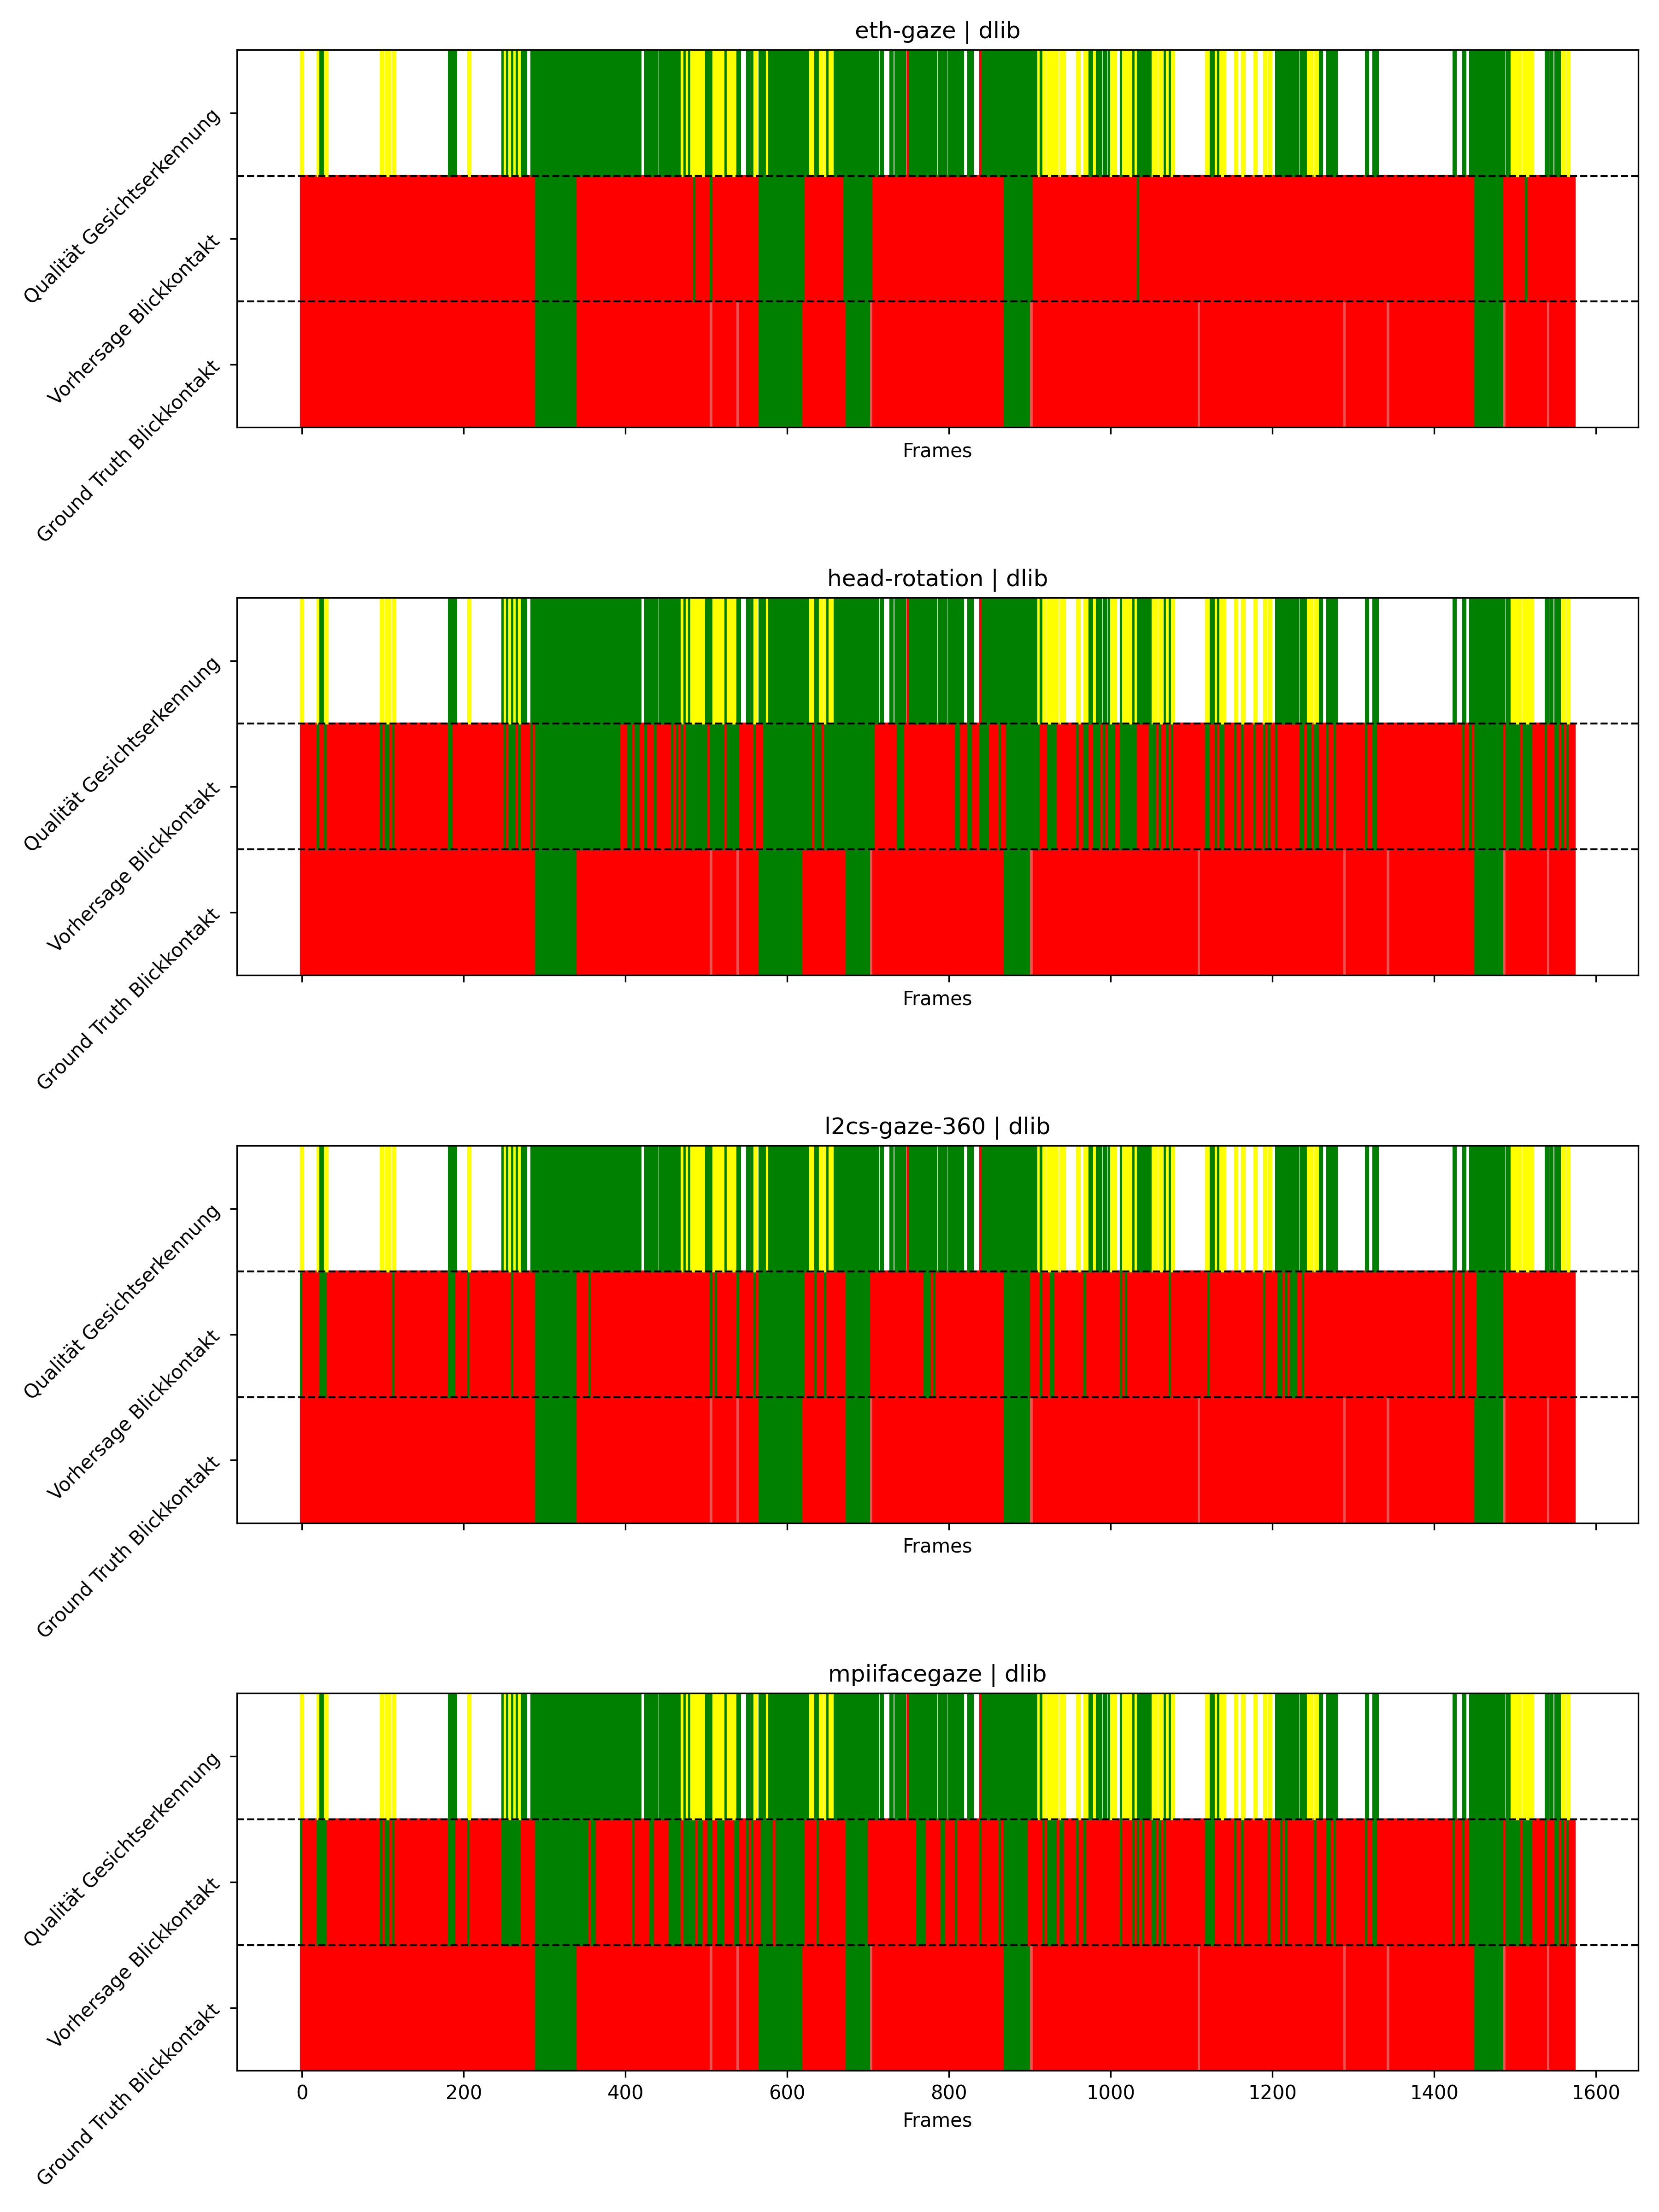
\includegraphics[width=1\linewidth]{appendix/04-dlib-overview-gaze.jpg}
\caption{Überblick über die Ground Truth des Blickkontakts, die Vorhersage des Blickkontakts und die Qualität der Gesichtserkennung mit \dlib. Die Bedeutung der Farben ist in Abbildung \ref{fig:evaluation:gaze:mpiifacegaze} erklärt.  }
\end{figure}

\begin{figure}[H]
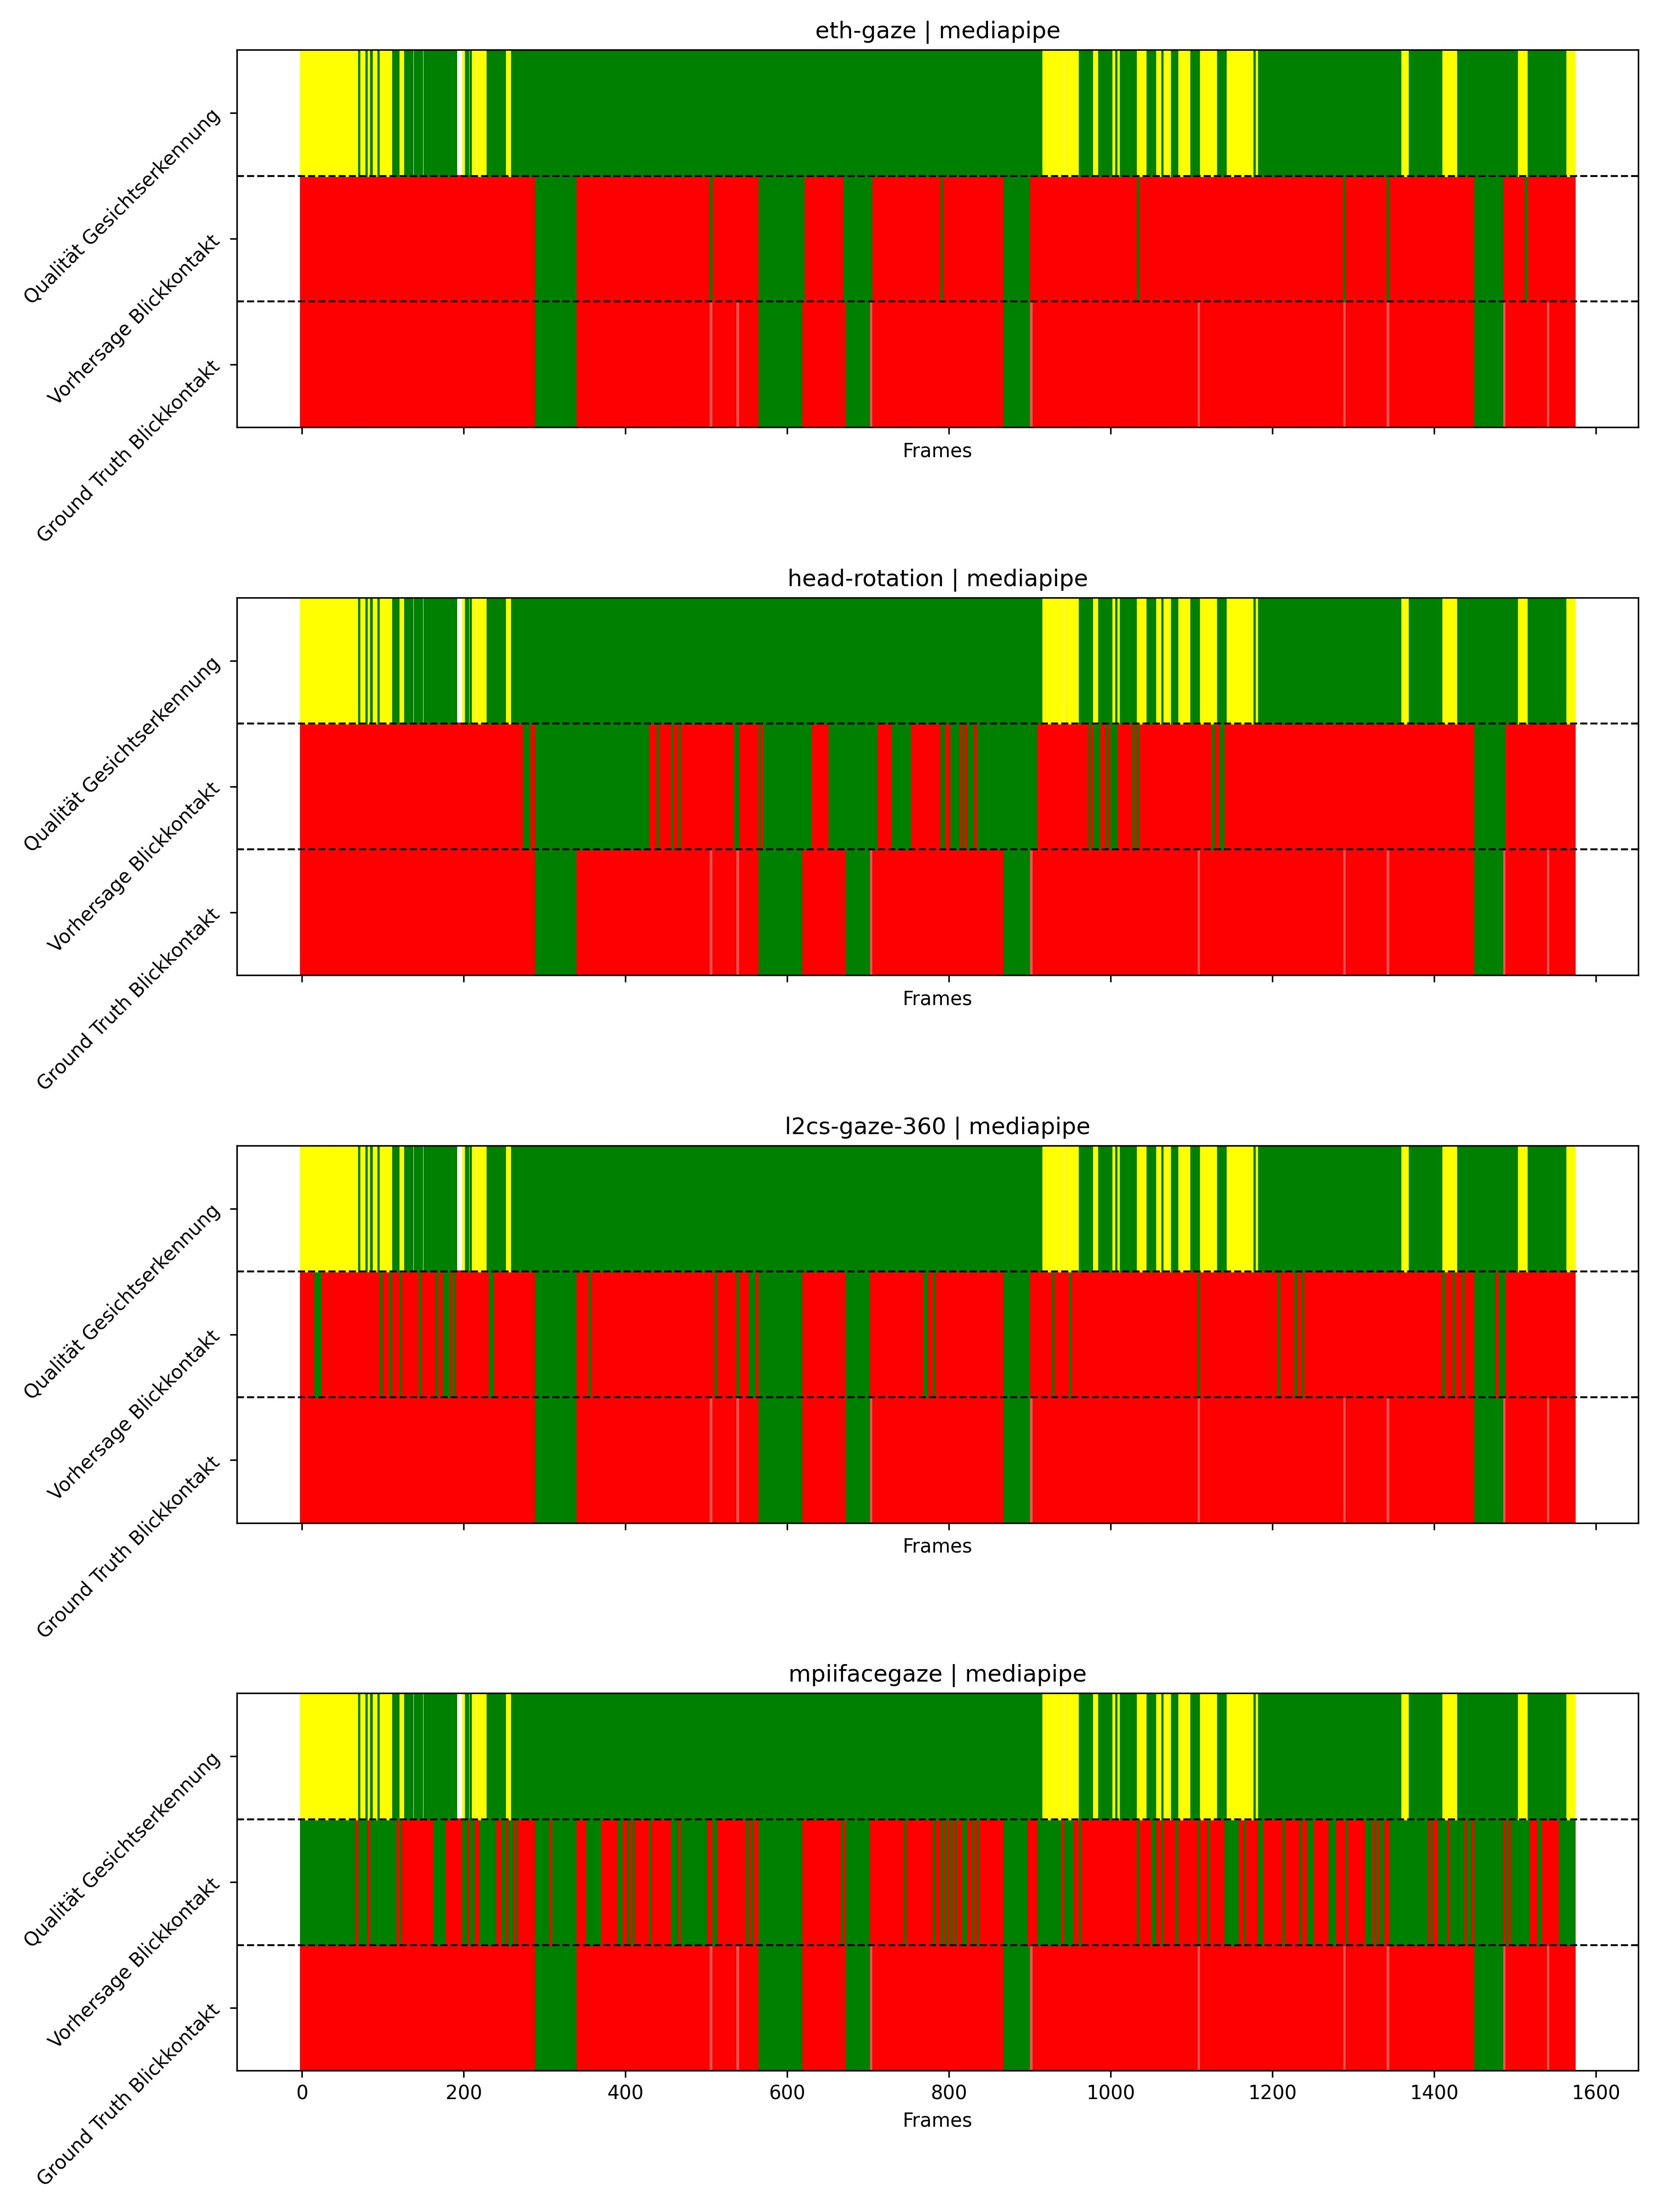
\includegraphics[width=1\linewidth]{appendix/04-mediapipe-overview-gaze.jpg}
\caption{Überblick über die Ground Truth des Blickkontakts, die Vorhersage des Blickkontakts und die Qualität der Gesichtserkennung mit \mediapipe. Die Bedeutung der Farben ist in Abbildung \ref{fig:evaluation:gaze:mpiifacegaze} erklärt.}
\end{figure}

\section{Video 05}
\begin{figure}[H]
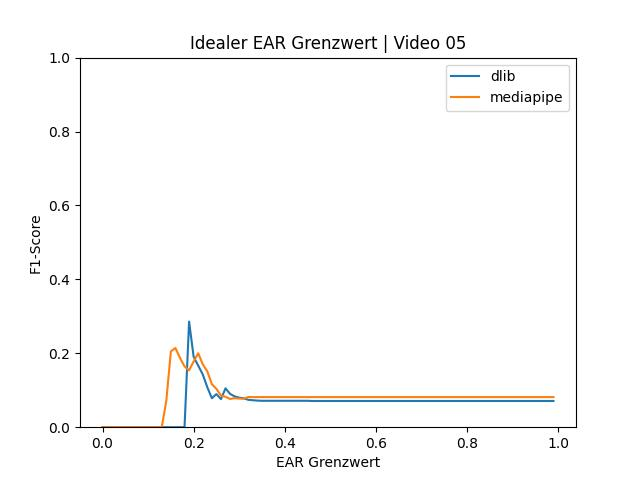
\includegraphics[width=0.7\linewidth]{appendix/05_f1-score-blink.jpg}
\caption{Ergebnisse der Bestimmung des idealen EAR-Grenzwerts für Video 05.}
\end{figure}

\begin{figure}[H]
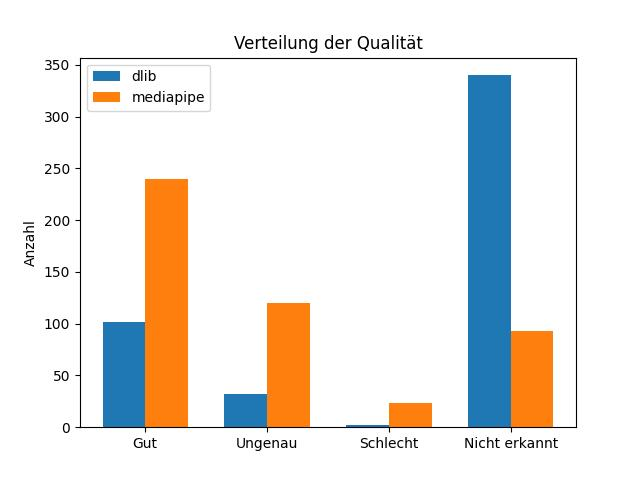
\includegraphics[width=0.7\linewidth]{appendix/05_bar-quality.jpg}
\caption{Aufteilung der Gesichtserkennungsqualität von Video 05.}
\end{figure}

\begin{table}[H]
\centering
\begin{tabular}{l|l|c c |c}
\toprule
\textbf{Gesichtserkennung} & \textbf{Blickrichtung} & \textbf{Seitenlänge} $\hitthresholdsize$ & \textbf{Verschiebung} $\hitthresholdposition$ & \textbf{F1-Score} \\ 
\midrule
\multirow{4}*{dlib}& ETH-XGaze & 0,122 & 0,01 & 0,942  \\ 
& Gaze360 & 0,459 & 0,059 & 0,84 \\ 
& MPIIFaceGaze & 0,082 & -0,027 & 0,75  \\ 
& Kopfrotation & 0,153 & 0,206 & 0,786  \\ 
\hline\multirow{4}*{MediaPipe}& ETH-XGaze & 0,153 & -0,002 & 0,989  \\ 
& Gaze360 & 0,357 & 0,047 & 0,792 \\ 
& MPIIFaceGaze & 0,031 & -0,027 & 0,538  \\ 
& Kopfrotation & 0,133 & 0,194 & 0,872  \\ 
\bottomrule\end{tabular}
\caption{Ergebnis des Hyperparameter-Tunings für die Zone speziell für Video 05.}
\label{tab:appendix:05:local}
\end{table}
\begin{table}[H]
\centering
\begin{tabular}{l|l|c c c c|c c|c}
\toprule
\textbf{Gesichtserkennung} & \textbf{Blickrichtung} & $TP$ & $TN$& $FP$ & $FN$ & \textbf{Precision} & \textbf{Recall} & \textbf{F1-Score} \\ 
\midrule
\multirow{4}*{dlib}& ETH-XGaze & 81 & 382 & 1 & 10 & 0,988 & 0,89 & 0,936 \\ 
& Gaze360 & 73 & 372 & 11 & 18 & 0,869 & 0,802 & 0,834 \\ 
& MPIIFaceGaze & 75 & 349 & 34 & 16 & 0,688 & 0,824 & 0,75 \\ 
& Kopfrotation & 77 & 353 & 30 & 14 & 0,72 & 0,846 & 0,778 \\ 
\hline\multirow{4}*{MediaPipe}& ETH-XGaze & 90 & 384 & 1 & 1 & 0,989 & 0,989 & 0,989 \\ 
& Gaze360 & 79 & 354 & 31 & 12 & 0,718 & 0,868 & 0,786 \\ 
& MPIIFaceGaze & 71 & 230 & 155 & 20 & 0,314 & 0,78 & 0,448 \\ 
& Kopfrotation & 80 & 367 & 18 & 11 & 0,816 & 0,879 & 0,847 \\ 
\bottomrule\end{tabular}
\caption{Zusammensetzung des F1-Scores unter Verwendung der in Kapitel \ref{sec:evaluation:results:gaze:threshold} bestimmten globalen Parameter $\hitthresholdsize$ und $\hitthresholdposition$.}
\label{tab:appendix:05:f1}
\end{table}
\begin{figure}[H]
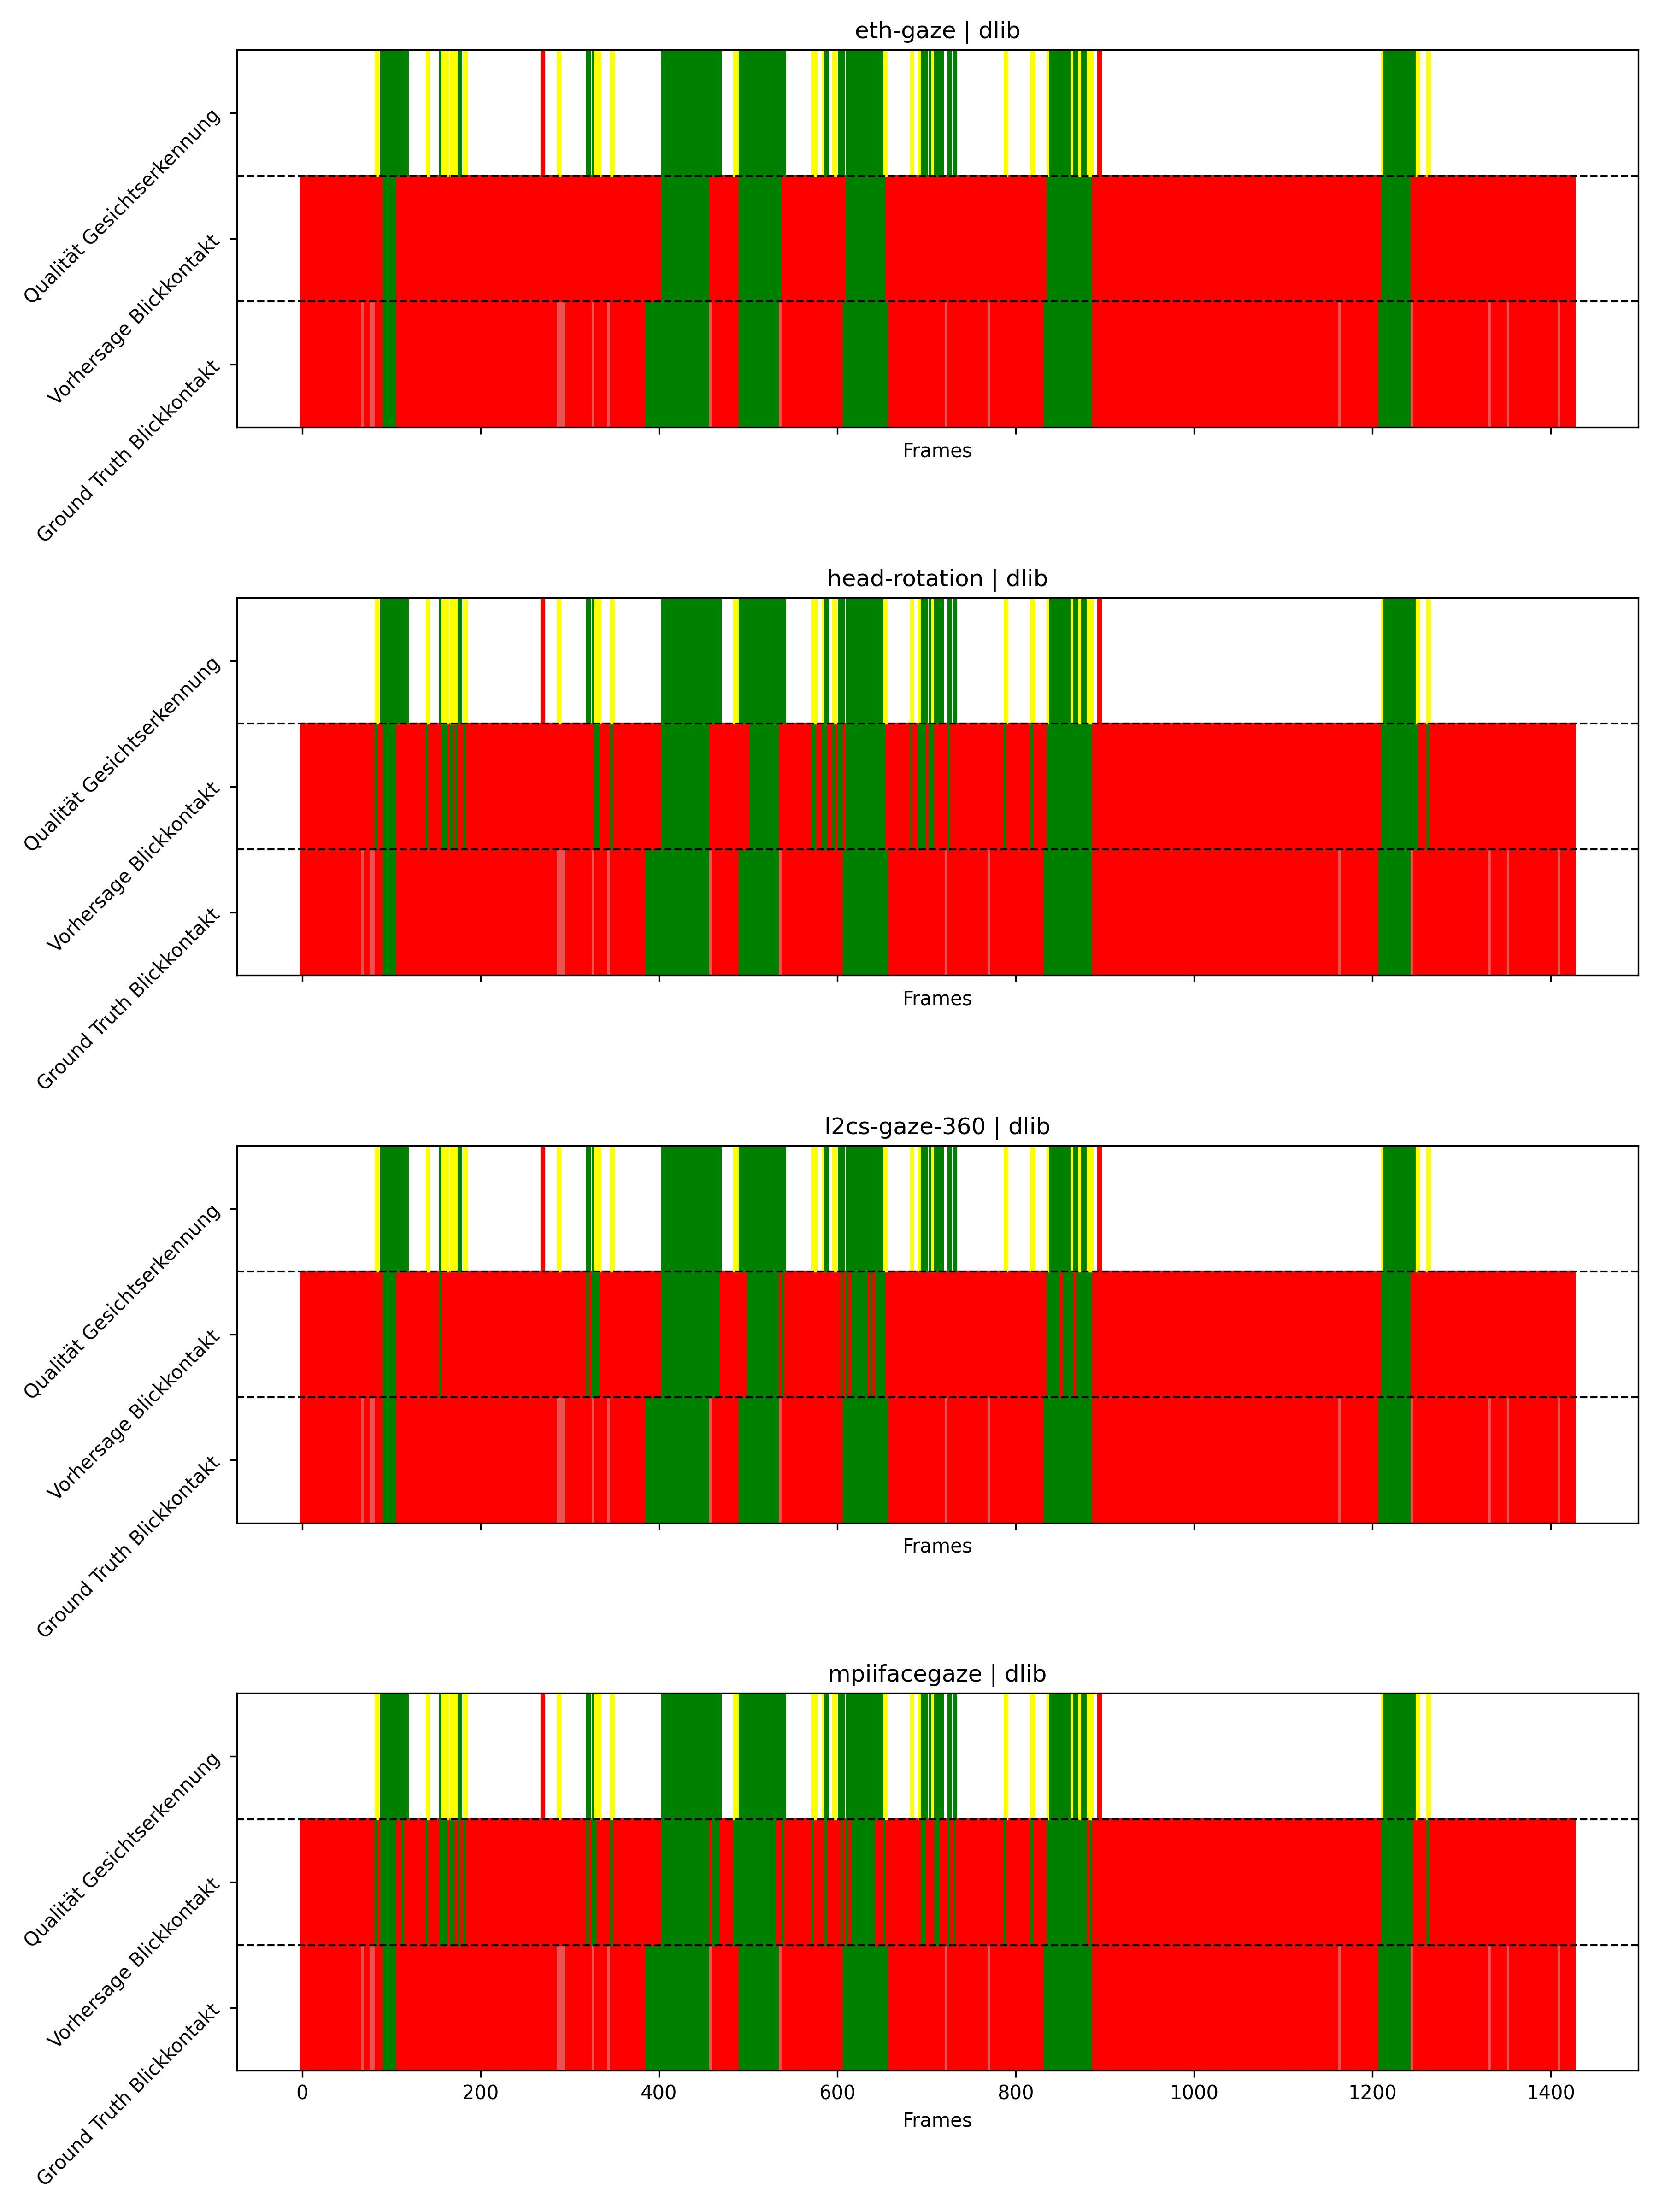
\includegraphics[width=1\linewidth]{appendix/05-dlib-overview-gaze.jpg}
\caption{Überblick über die Ground Truth des Blickkontakts, die Vorhersage des Blickkontakts und die Qualität der Gesichtserkennung mit \dlib. Die Bedeutung der Farben ist in Abbildung \ref{fig:evaluation:gaze:mpiifacegaze} erklärt.  }
\end{figure}

\begin{figure}[H]
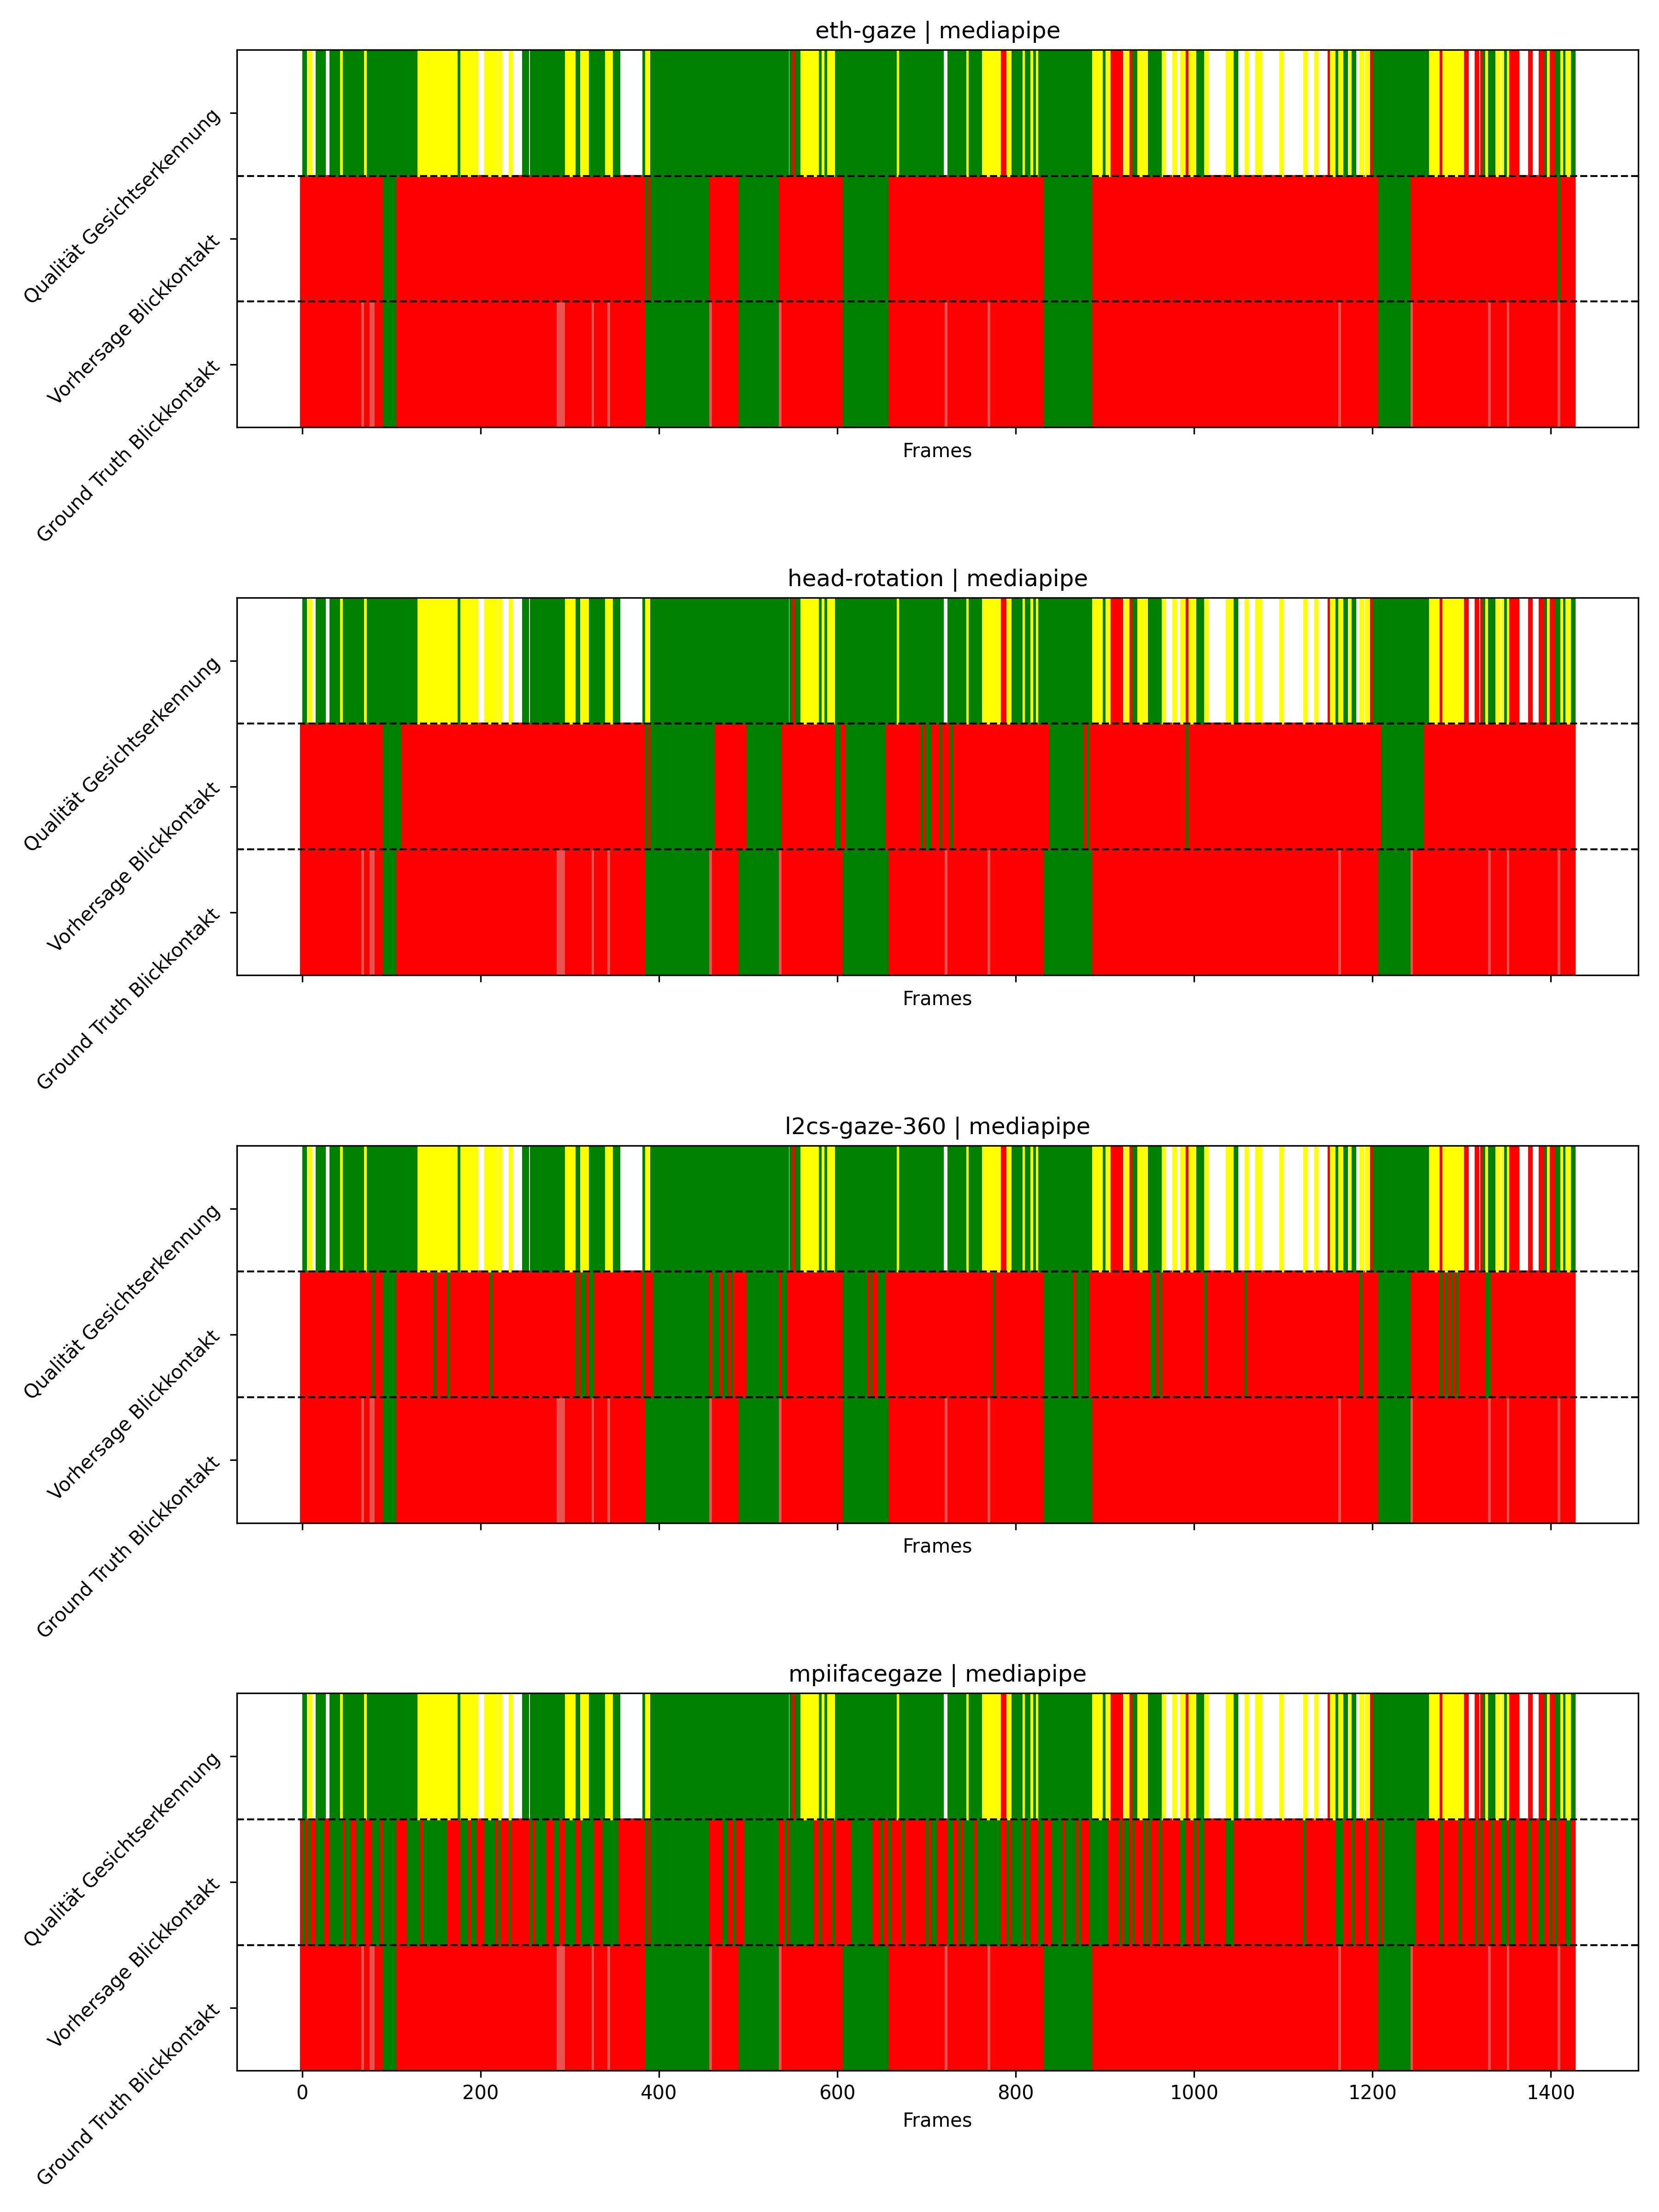
\includegraphics[width=1\linewidth]{appendix/05-mediapipe-overview-gaze.jpg}
\caption{Überblick über die Ground Truth des Blickkontakts, die Vorhersage des Blickkontakts und die Qualität der Gesichtserkennung mit \mediapipe. Die Bedeutung der Farben ist in Abbildung \ref{fig:evaluation:gaze:mpiifacegaze} erklärt.}
\end{figure}

\section{Video 06}
\begin{figure}[H]
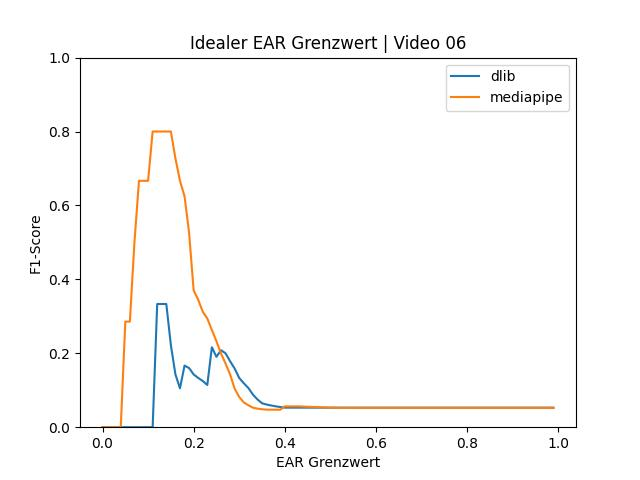
\includegraphics[width=0.7\linewidth]{appendix/06_f1-score-blink.jpg}
\caption{Ergebnisse der Bestimmung des idealen EAR-Grenzwerts für Video 06.}
\end{figure}

\begin{figure}[H]
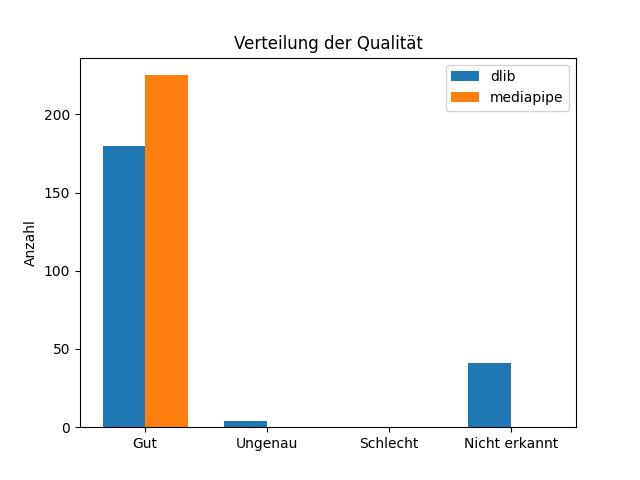
\includegraphics[width=0.7\linewidth]{appendix/06_bar-quality.jpg}
\caption{Aufteilung der Gesichtserkennungsqualität von Video 06.}
\end{figure}

\begin{table}[H]
\centering
\begin{tabular}{l|l|c c |c}
\toprule
\textbf{Gesichtserkennung} & \textbf{Blickrichtung} & \textbf{Seitenlänge} $\hitthresholdsize$ & \textbf{Verschiebung} $\hitthresholdposition$ & \textbf{F1-Score} \\ 
\midrule
\multirow{4}*{dlib}& ETH-XGaze & 0,092 & -0,027 & 0,991  \\ 
& Gaze360 & 0,276 & 0,231 & 0,842 \\ 
& MPIIFaceGaze & 0,041 & -0,027 & 0,831  \\ 
& Kopfrotation & 0,112 & 0,108 & 0,573  \\ 
\hline\multirow{4}*{MediaPipe}& ETH-XGaze & 0,173 & 0,01 & 0,982  \\ 
& Gaze360 & 0,133 & 0,047 & 0,876 \\ 
& MPIIFaceGaze & 0,041 & -0,027 & 0,895  \\ 
& Kopfrotation & 0,112 & 0,12 & 0,568  \\ 
\bottomrule\end{tabular}
\caption{Ergebnis des Hyperparameter-Tunings für die Zone speziell für Video 06.}
\label{tab:appendix:06:local}
\end{table}
\begin{table}[H]
\centering
\begin{tabular}{l|l|c c c c|c c|c}
\toprule
\textbf{Gesichtserkennung} & \textbf{Blickrichtung} & $TP$ & $TN$& $FP$ & $FN$ & \textbf{Precision} & \textbf{Recall} & \textbf{F1-Score} \\ 
\midrule
\multirow{4}*{dlib}& ETH-XGaze & 55 & 158 & 12 & 0 & 0,821 & 1,0 & 0,902 \\ 
& Gaze360 & 53 & 107 & 63 & 2 & 0,457 & 0,964 & 0,62 \\ 
& MPIIFaceGaze & 55 & 104 & 66 & 0 & 0,455 & 1,0 & 0,625 \\ 
& Kopfrotation & 55 & 59 & 111 & 0 & 0,331 & 1,0 & 0,498 \\ 
\hline\multirow{4}*{MediaPipe}& ETH-XGaze & 55 & 138 & 32 & 0 & 0,632 & 1,0 & 0,775 \\ 
& Gaze360 & 53 & 126 & 44 & 2 & 0,546 & 0,964 & 0,697 \\ 
& MPIIFaceGaze & 55 & 153 & 17 & 0 & 0,764 & 1,0 & 0,866 \\ 
& Kopfrotation & 55 & 60 & 110 & 0 & 0,333 & 1,0 & 0,5 \\ 
\bottomrule\end{tabular}
\caption{Zusammensetzung des F1-Scores unter Verwendung der in Kapitel \ref{sec:evaluation:results:gaze:threshold} bestimmten globalen Parameter $\hitthresholdsize$ und $\hitthresholdposition$.}
\label{tab:appendix:06:f1}
\end{table}
\begin{figure}[H]
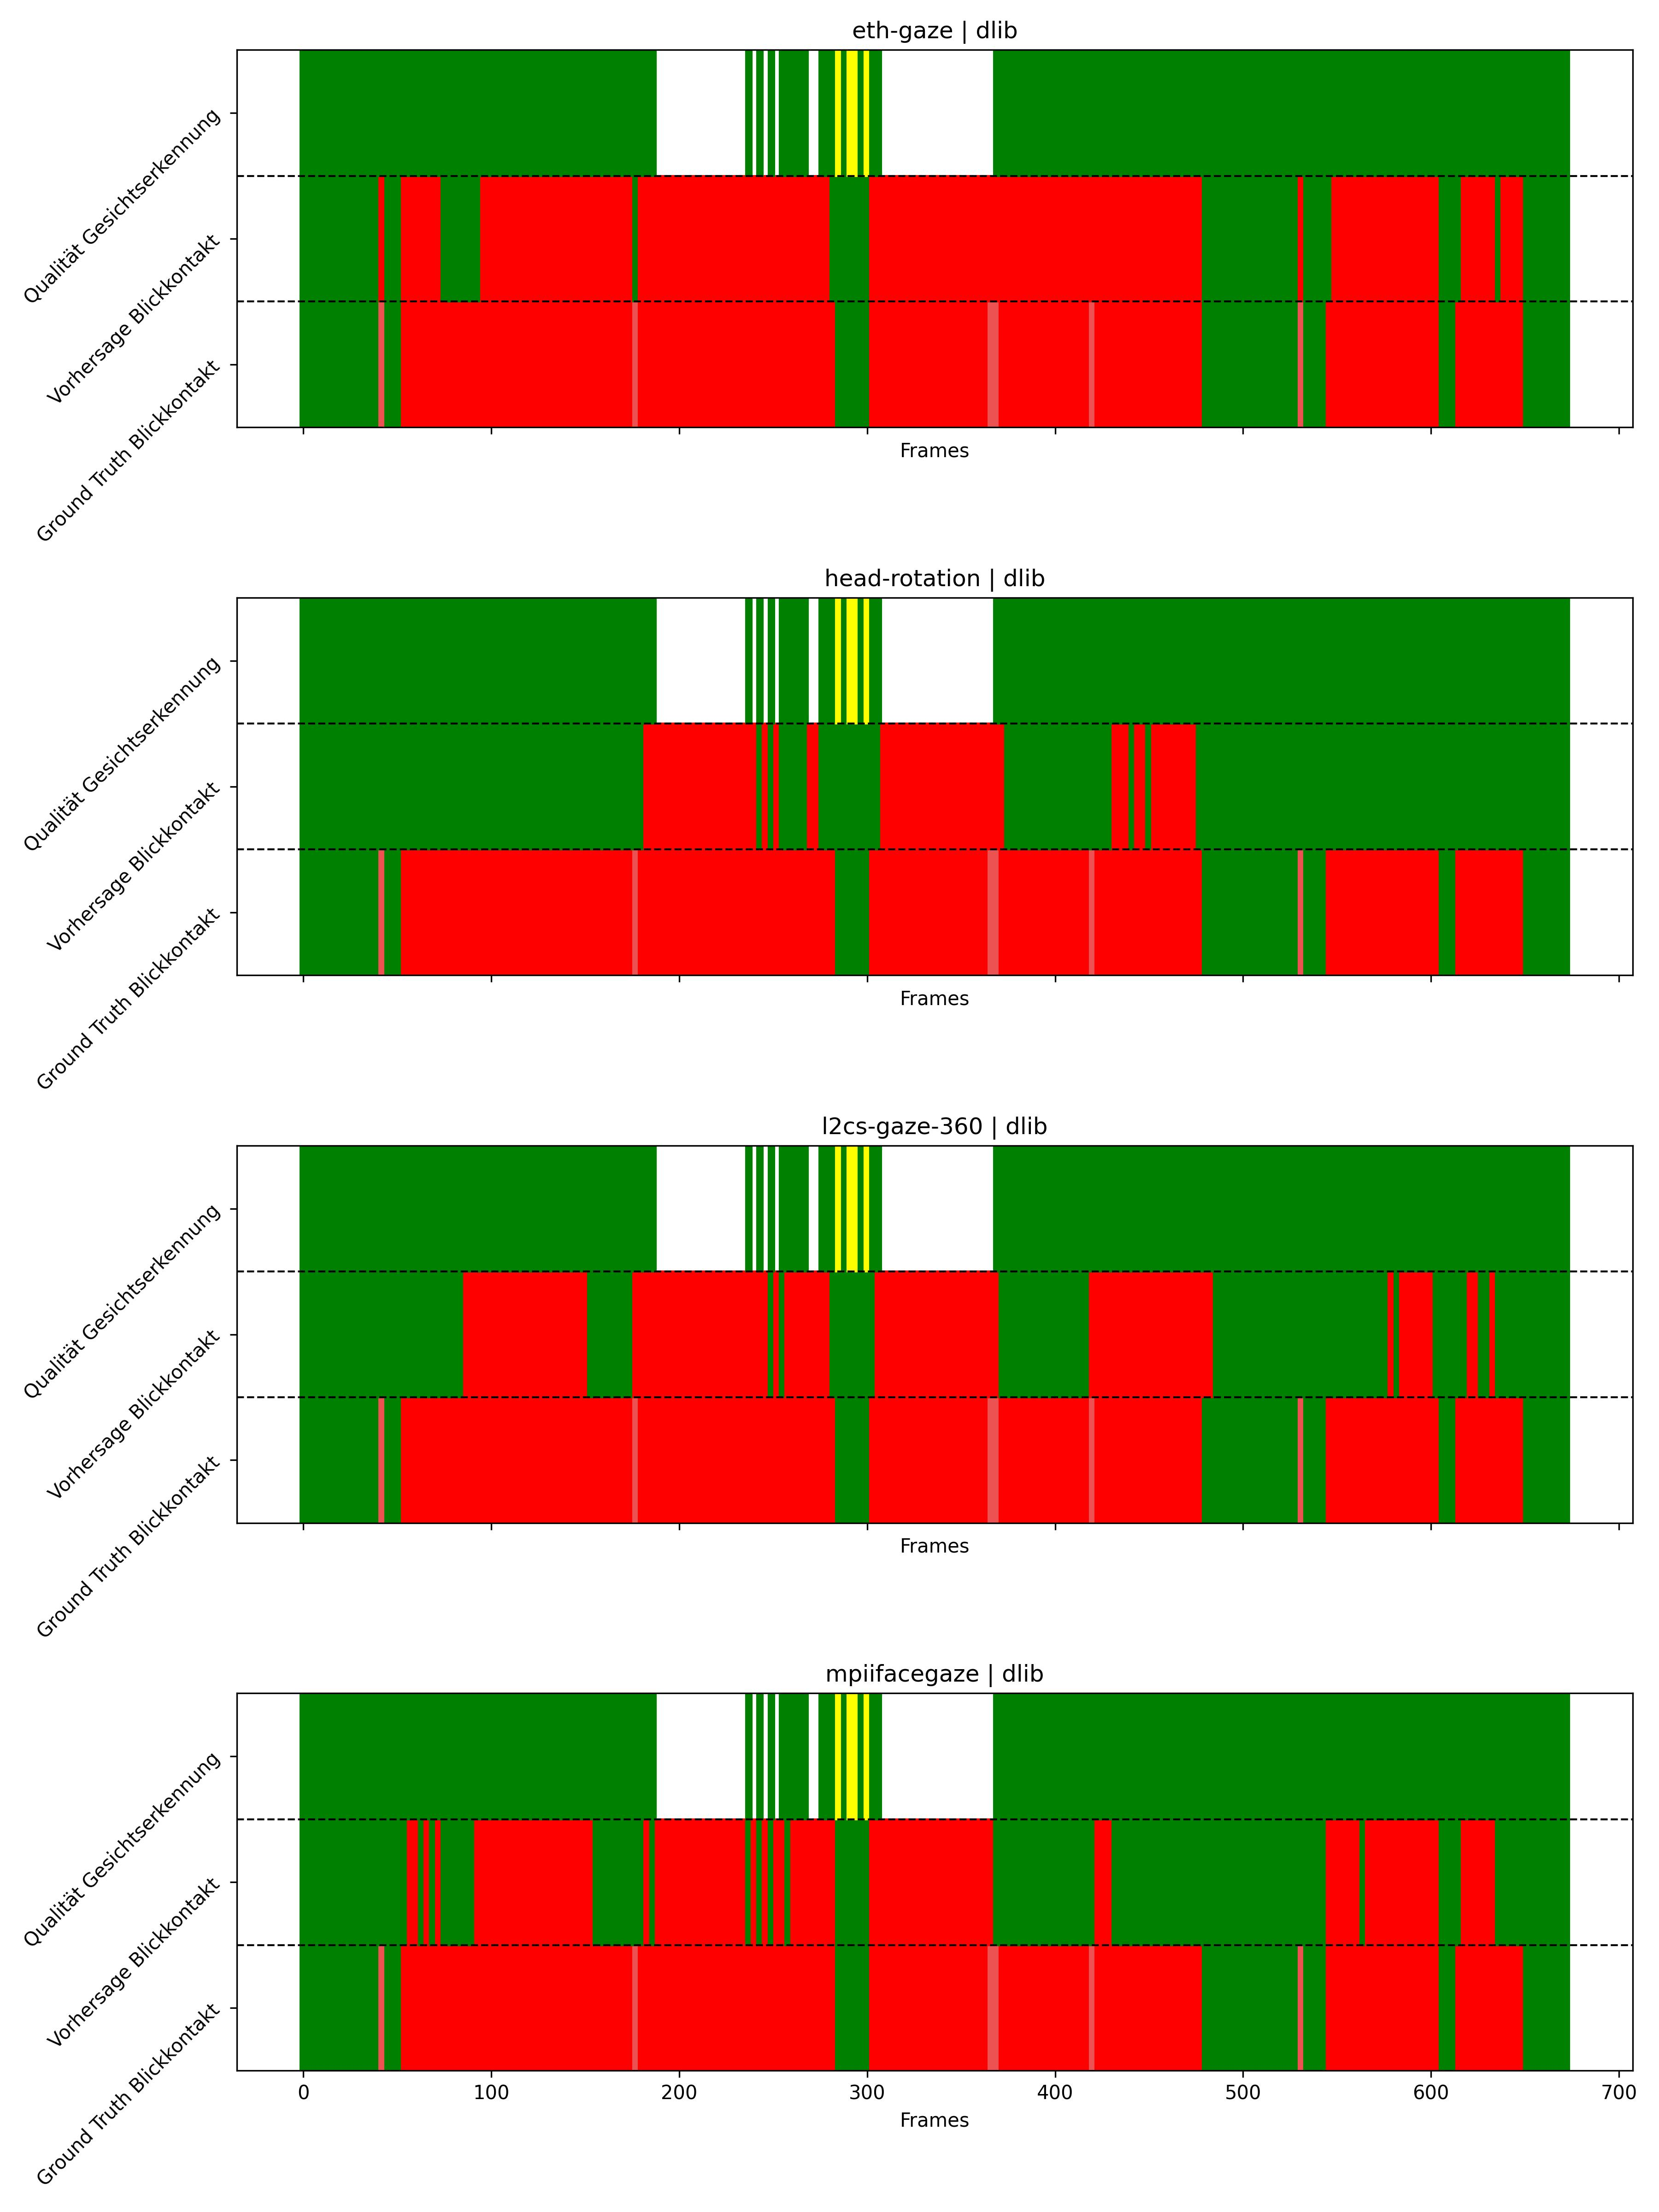
\includegraphics[width=1\linewidth]{appendix/06-dlib-overview-gaze.jpg}
\caption{Überblick über die Ground Truth des Blickkontakts, die Vorhersage des Blickkontakts und die Qualität der Gesichtserkennung mit \dlib. Die Bedeutung der Farben ist in Abbildung \ref{fig:evaluation:gaze:mpiifacegaze} erklärt.  }
\end{figure}

\begin{figure}[H]
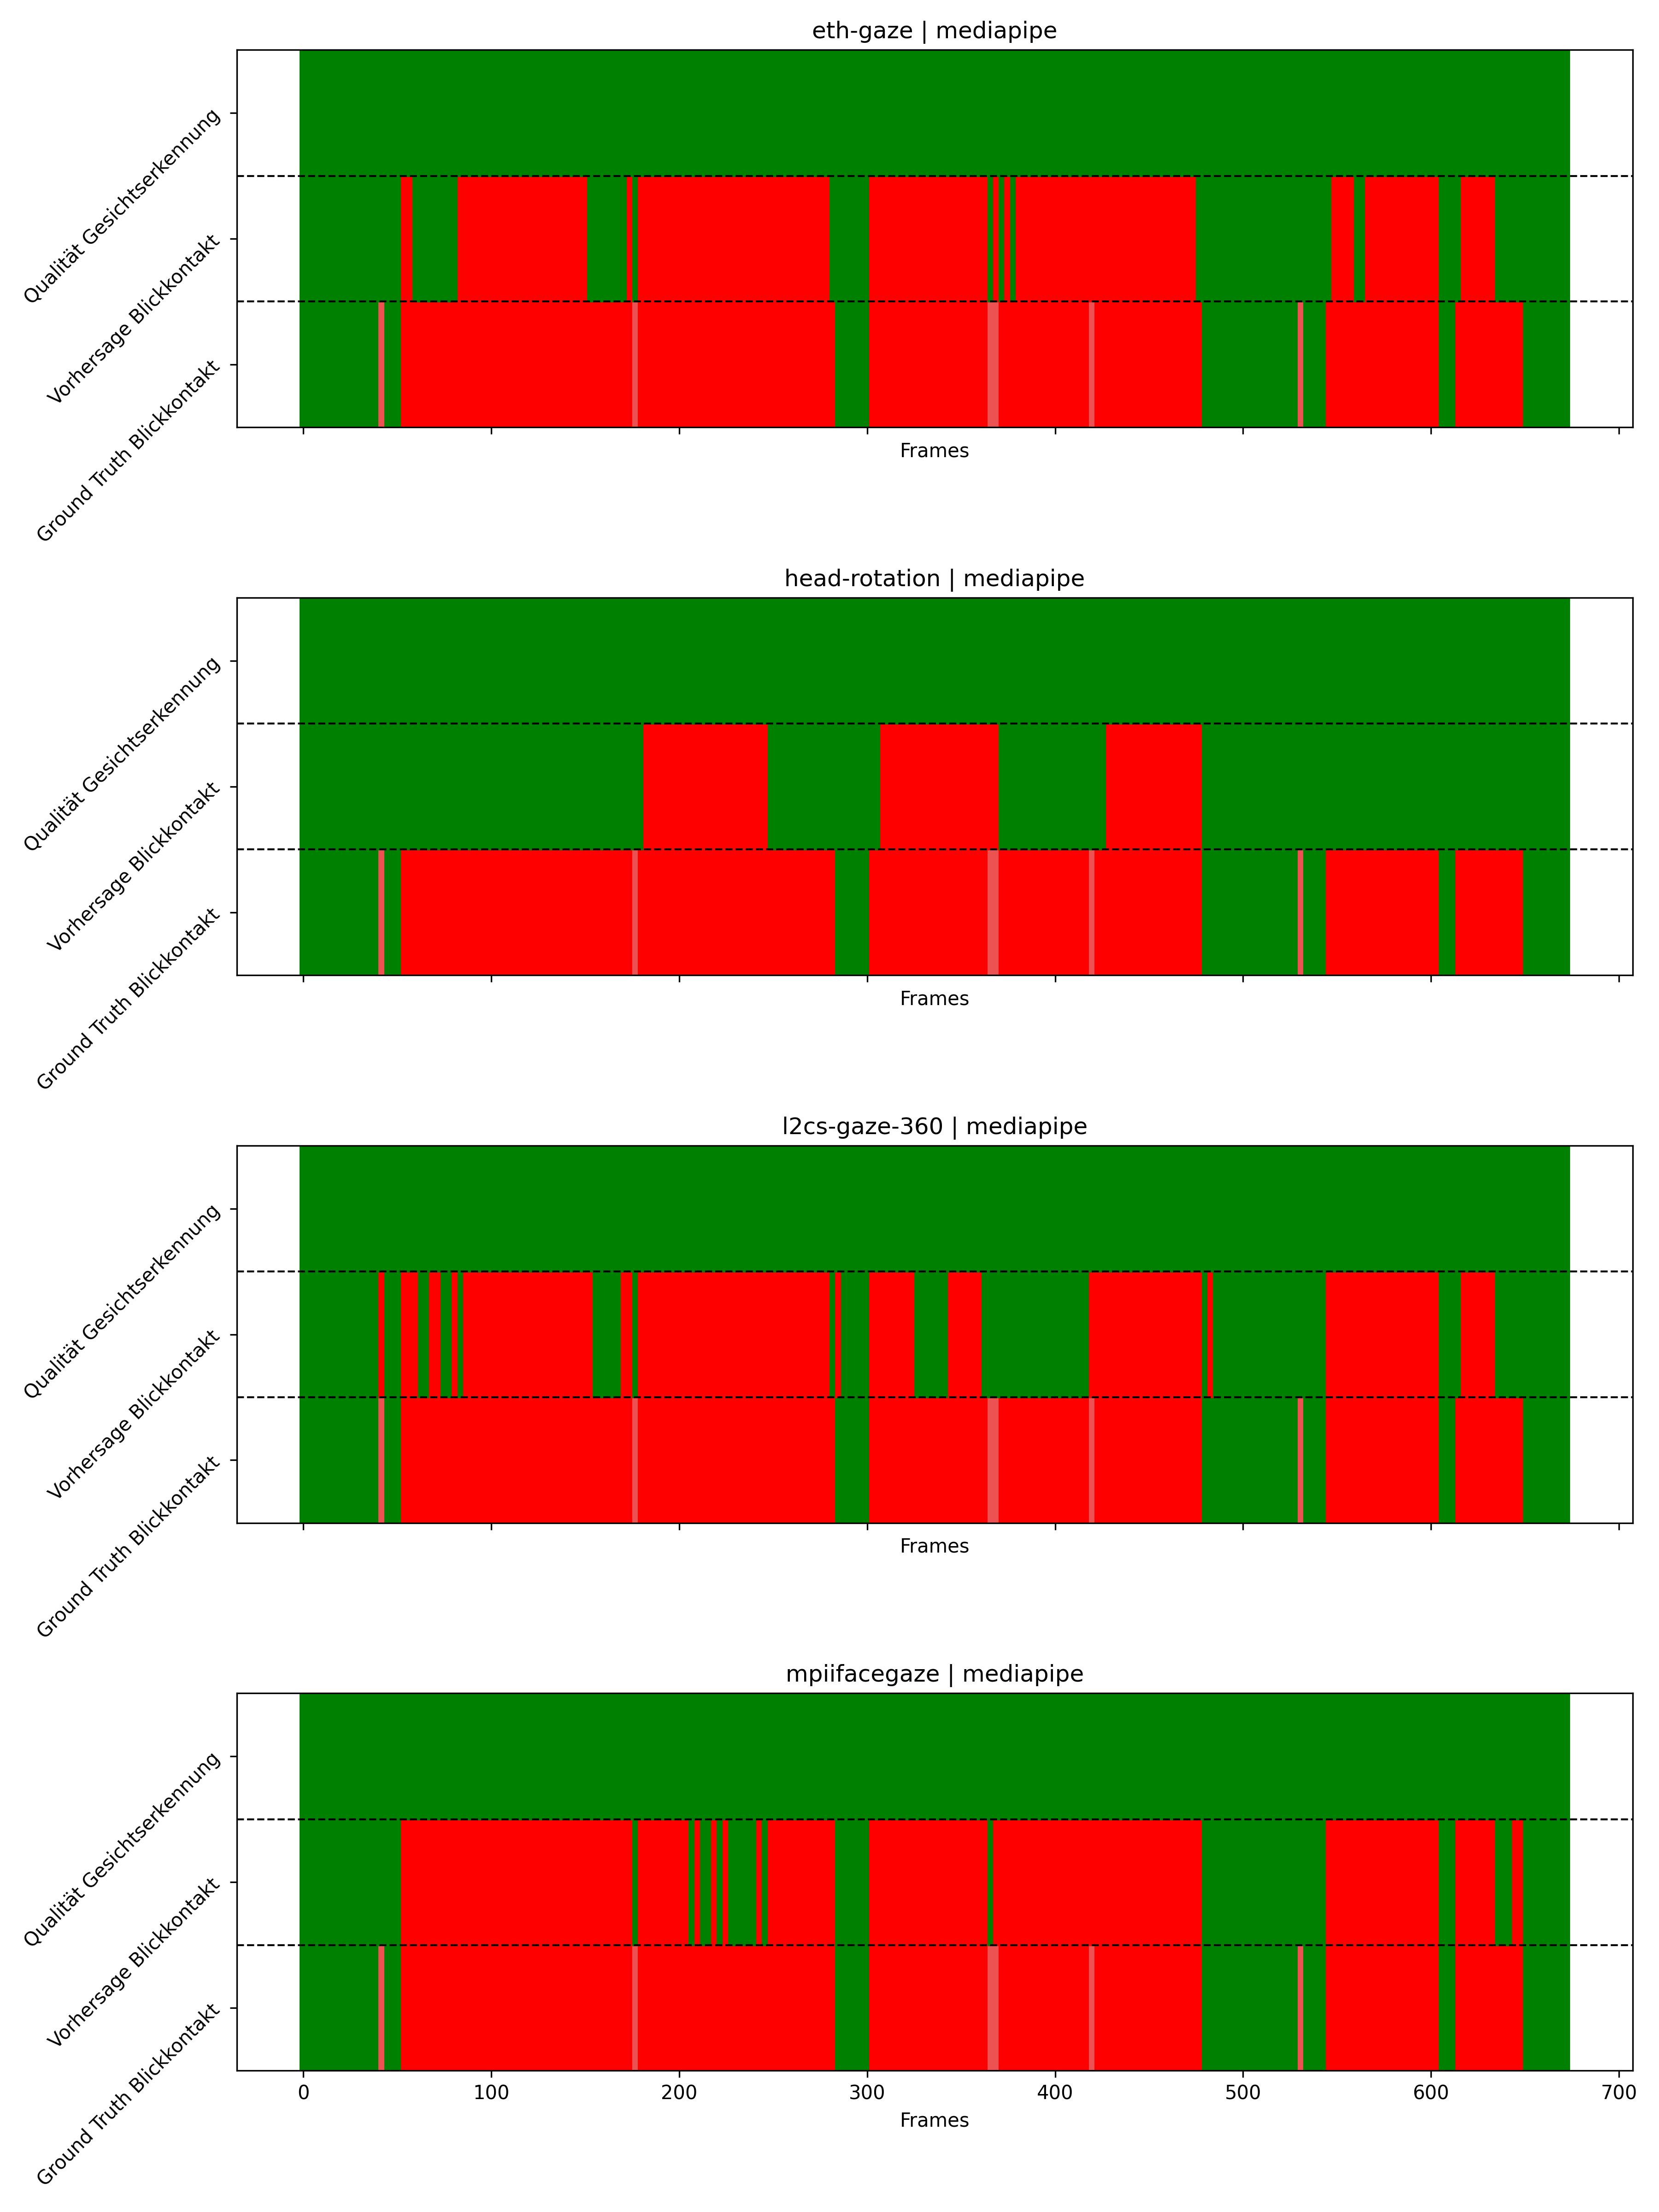
\includegraphics[width=1\linewidth]{appendix/06-mediapipe-overview-gaze.jpg}
\caption{Überblick über die Ground Truth des Blickkontakts, die Vorhersage des Blickkontakts und die Qualität der Gesichtserkennung mit \mediapipe. Die Bedeutung der Farben ist in Abbildung \ref{fig:evaluation:gaze:mpiifacegaze} erklärt.}
\end{figure}

\section{Video 07}
\begin{figure}[H]
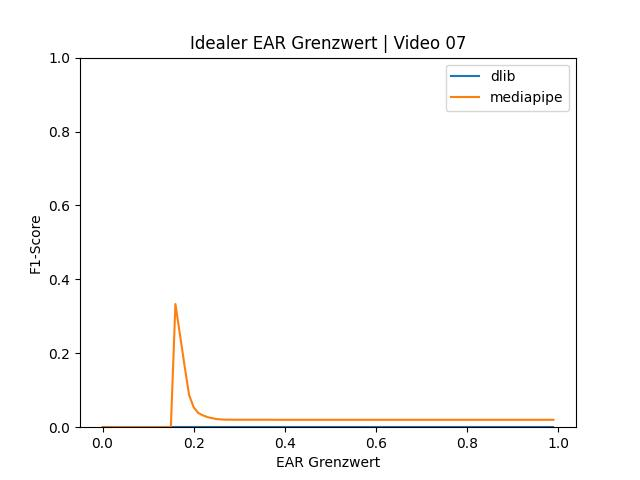
\includegraphics[width=0.7\linewidth]{appendix/07_f1-score-blink.jpg}
\caption{Ergebnisse der Bestimmung des idealen EAR-Grenzwerts für Video 07.}
\end{figure}

\begin{figure}[H]
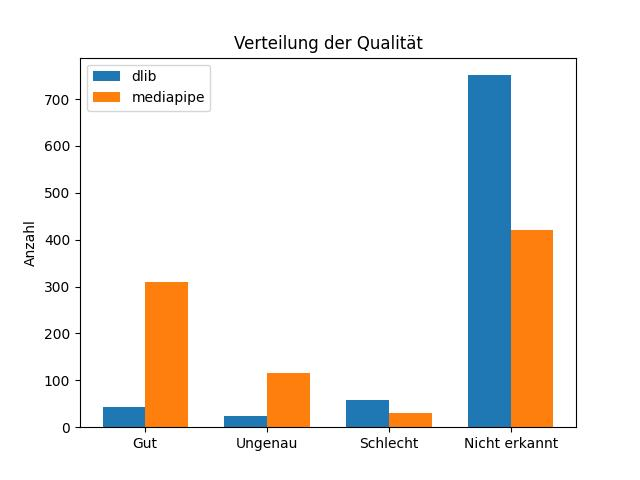
\includegraphics[width=0.7\linewidth]{appendix/07_bar-quality.jpg}
\caption{Aufteilung der Gesichtserkennungsqualität von Video 07.}
\end{figure}

\begin{table}[H]
\centering
\begin{tabular}{l|l|c c |c}
\toprule
\textbf{Gesichtserkennung} & \textbf{Blickrichtung} & \textbf{Seitenlänge} $\hitthresholdsize$ & \textbf{Verschiebung} $\hitthresholdposition$ & \textbf{F1-Score} \\ 
\midrule
\multirow{4}*{dlib}& ETH-XGaze & 0,357 & 0,059 & 0,626  \\ 
& Gaze360 & 0,5 & 0,084 & 0,435 \\ 
& MPIIFaceGaze & 0,102 & 0,035 & 0,581  \\ 
& Kopfrotation & 0,235 & 0,292 & 0,575  \\ 
\hline\multirow{4}*{MediaPipe}& ETH-XGaze & 0,296 & 0,084 & 0,786  \\ 
& Gaze360 & 0,5 & 0,071 & 0,4 \\ 
& MPIIFaceGaze & 0,112 & 0,059 & 0,788  \\ 
& Kopfrotation & 0,184 & 0,292 & 0,9  \\ 
\bottomrule\end{tabular}
\caption{Ergebnis des Hyperparameter-Tunings für die Zone speziell für Video 07.}
\label{tab:appendix:07:local}
\end{table}
\begin{table}[H]
\centering
\begin{tabular}{l|l|c c c c|c c|c}
\toprule
\textbf{Gesichtserkennung} & \textbf{Blickrichtung} & $TP$ & $TN$& $FP$ & $FN$ & \textbf{Precision} & \textbf{Recall} & \textbf{F1-Score} \\ 
\midrule
\multirow{4}*{dlib}& ETH-XGaze & 25 & 758 & 4 & 88 & 0,862 & 0,221 & 0,352 \\ 
& Gaze360 & 30 & 742 & 20 & 83 & 0,6 & 0,265 & 0,368 \\ 
& MPIIFaceGaze & 42 & 712 & 50 & 71 & 0,457 & 0,372 & 0,41 \\ 
& Kopfrotation & 35 & 717 & 45 & 78 & 0,438 & 0,31 & 0,363 \\ 
\hline\multirow{4}*{MediaPipe}& ETH-XGaze & 56 & 736 & 26 & 57 & 0,683 & 0,496 & 0,574 \\ 
& Gaze360 & 46 & 638 & 124 & 67 & 0,271 & 0,407 & 0,325 \\ 
& MPIIFaceGaze & 56 & 671 & 91 & 57 & 0,381 & 0,496 & 0,431 \\ 
& Kopfrotation & 33 & 762 & 0 & 80 & 1,0 & 0,292 & 0,452 \\ 
\bottomrule\end{tabular}
\caption{Zusammensetzung des F1-Scores unter Verwendung der in Kapitel \ref{sec:evaluation:results:gaze:threshold} bestimmten globalen Parameter $\hitthresholdsize$ und $\hitthresholdposition$.}
\label{tab:appendix:07:f1}
\end{table}
\begin{figure}[H]
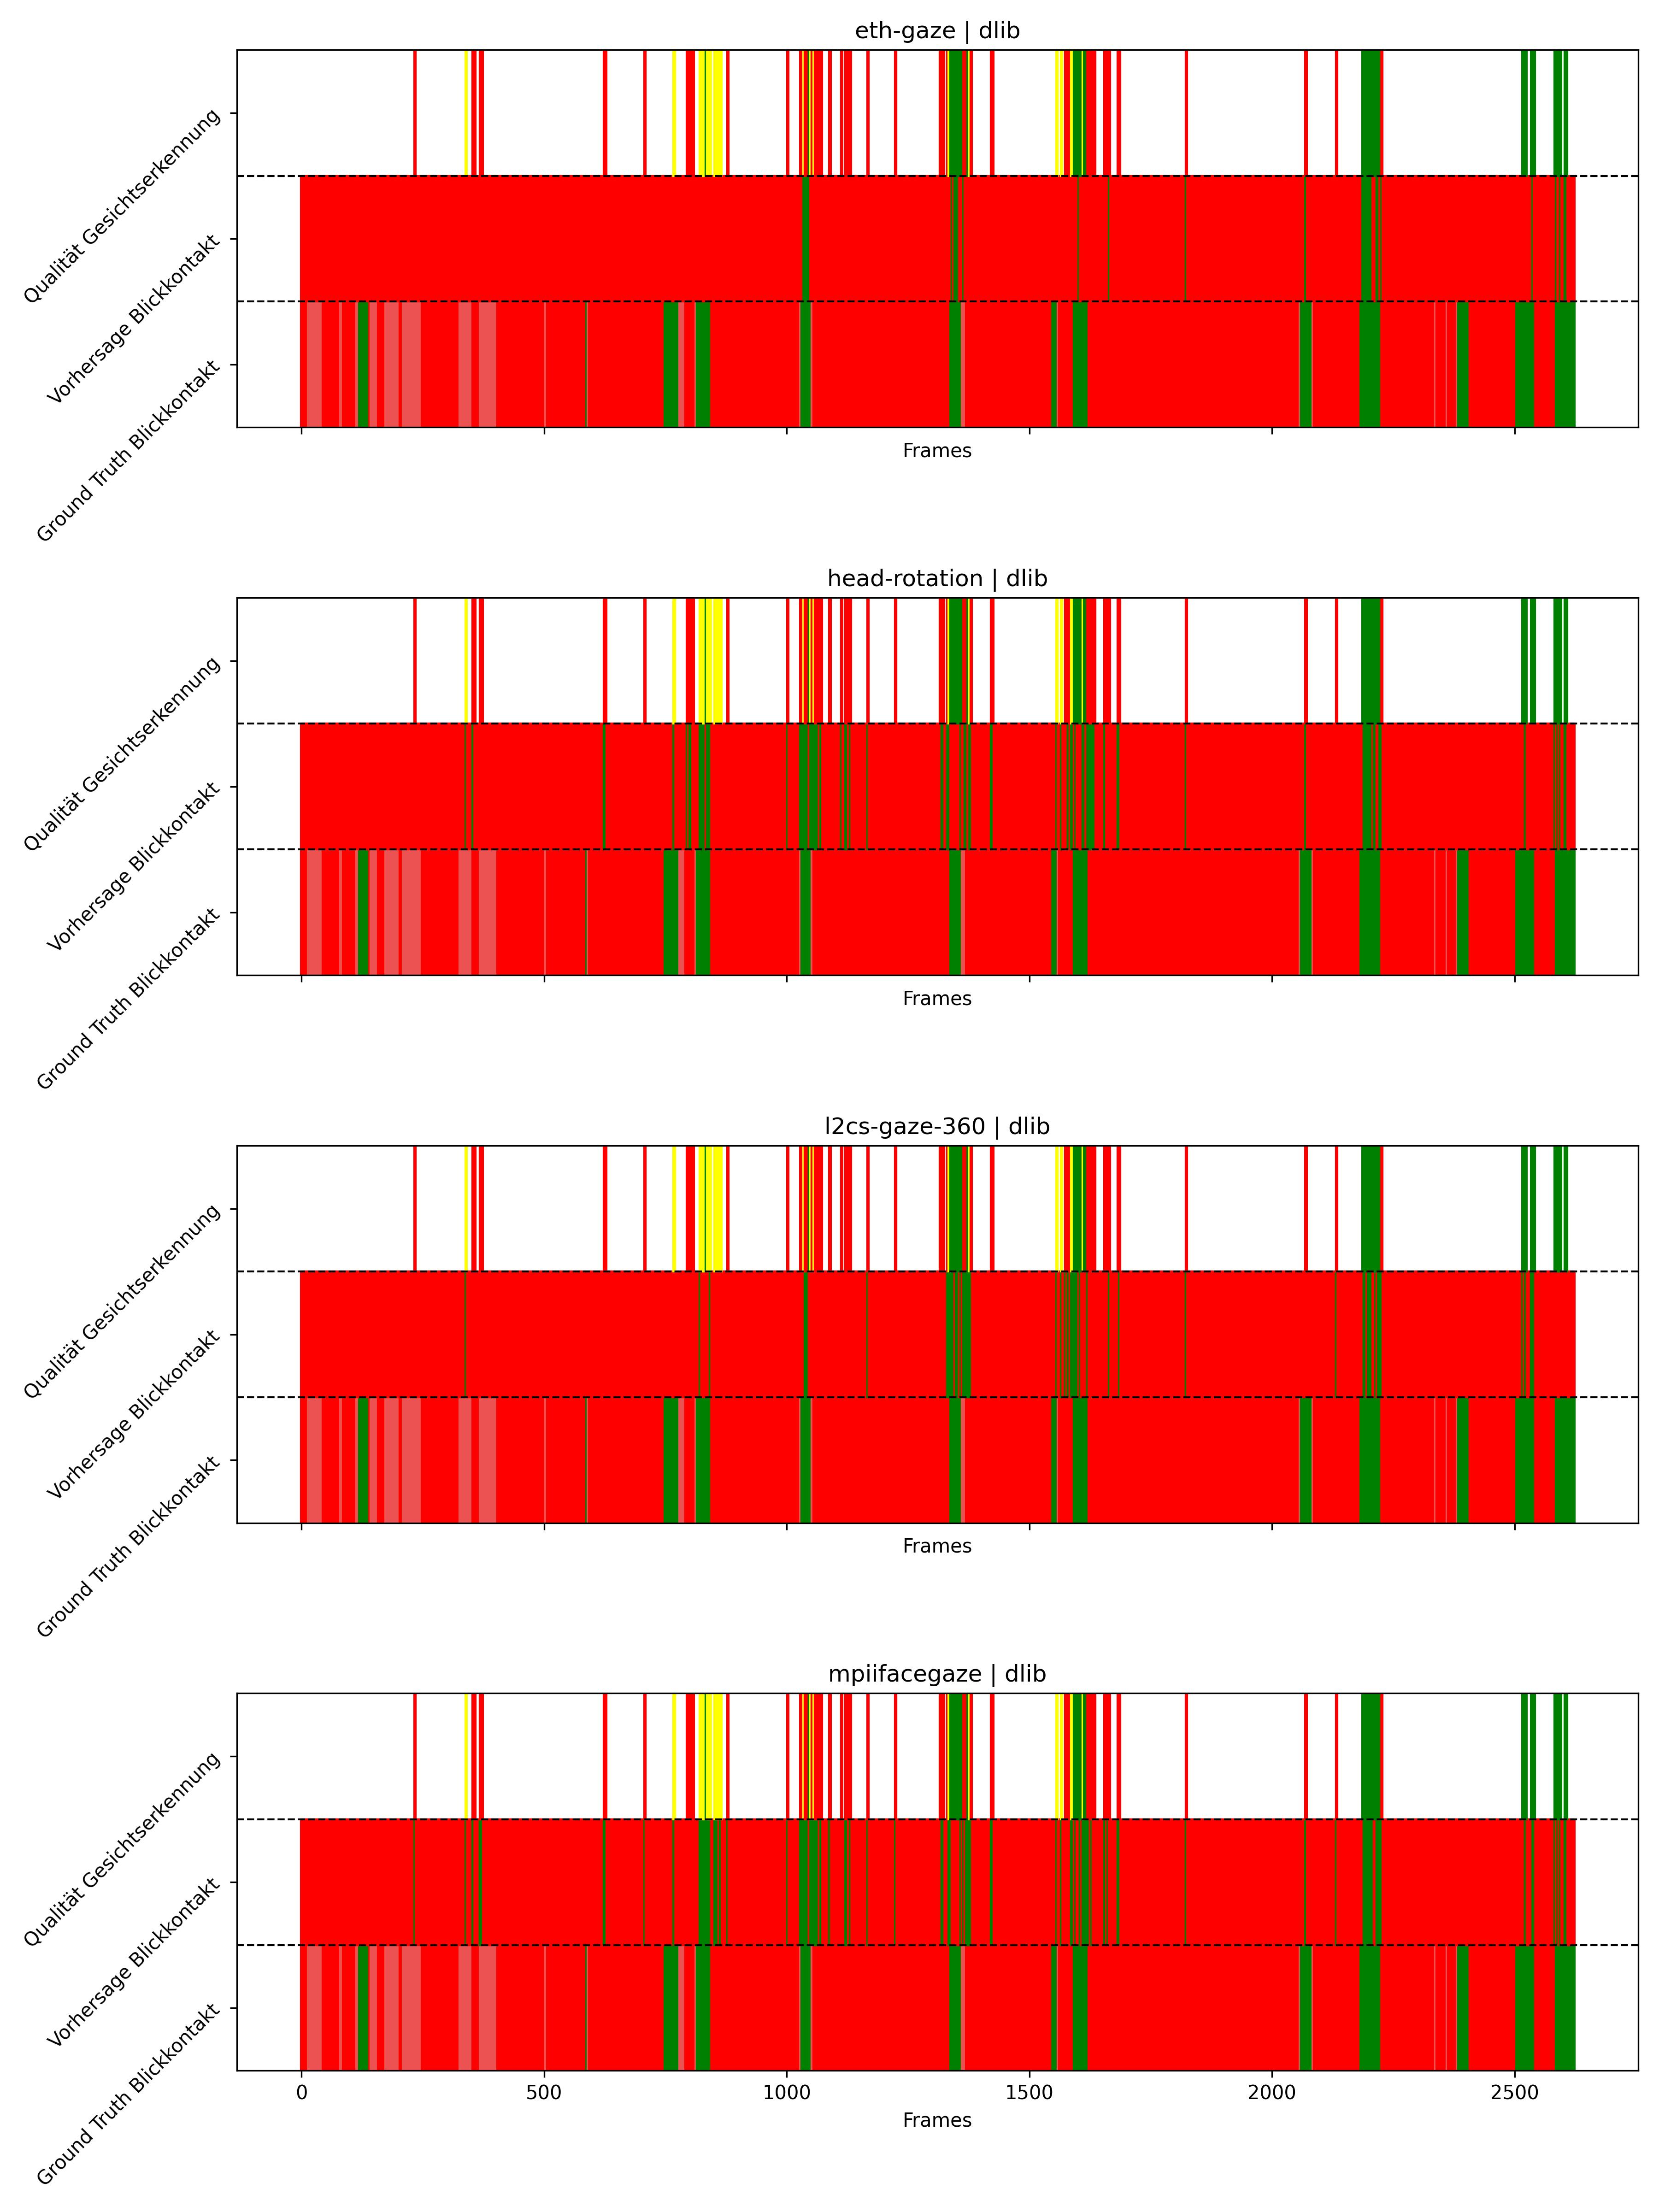
\includegraphics[width=1\linewidth]{appendix/07-dlib-overview-gaze.jpg}
\caption{Überblick über die Ground Truth des Blickkontakts, die Vorhersage des Blickkontakts und die Qualität der Gesichtserkennung mit \dlib. Die Bedeutung der Farben ist in Abbildung \ref{fig:evaluation:gaze:mpiifacegaze} erklärt.  }
\end{figure}

\begin{figure}[H]
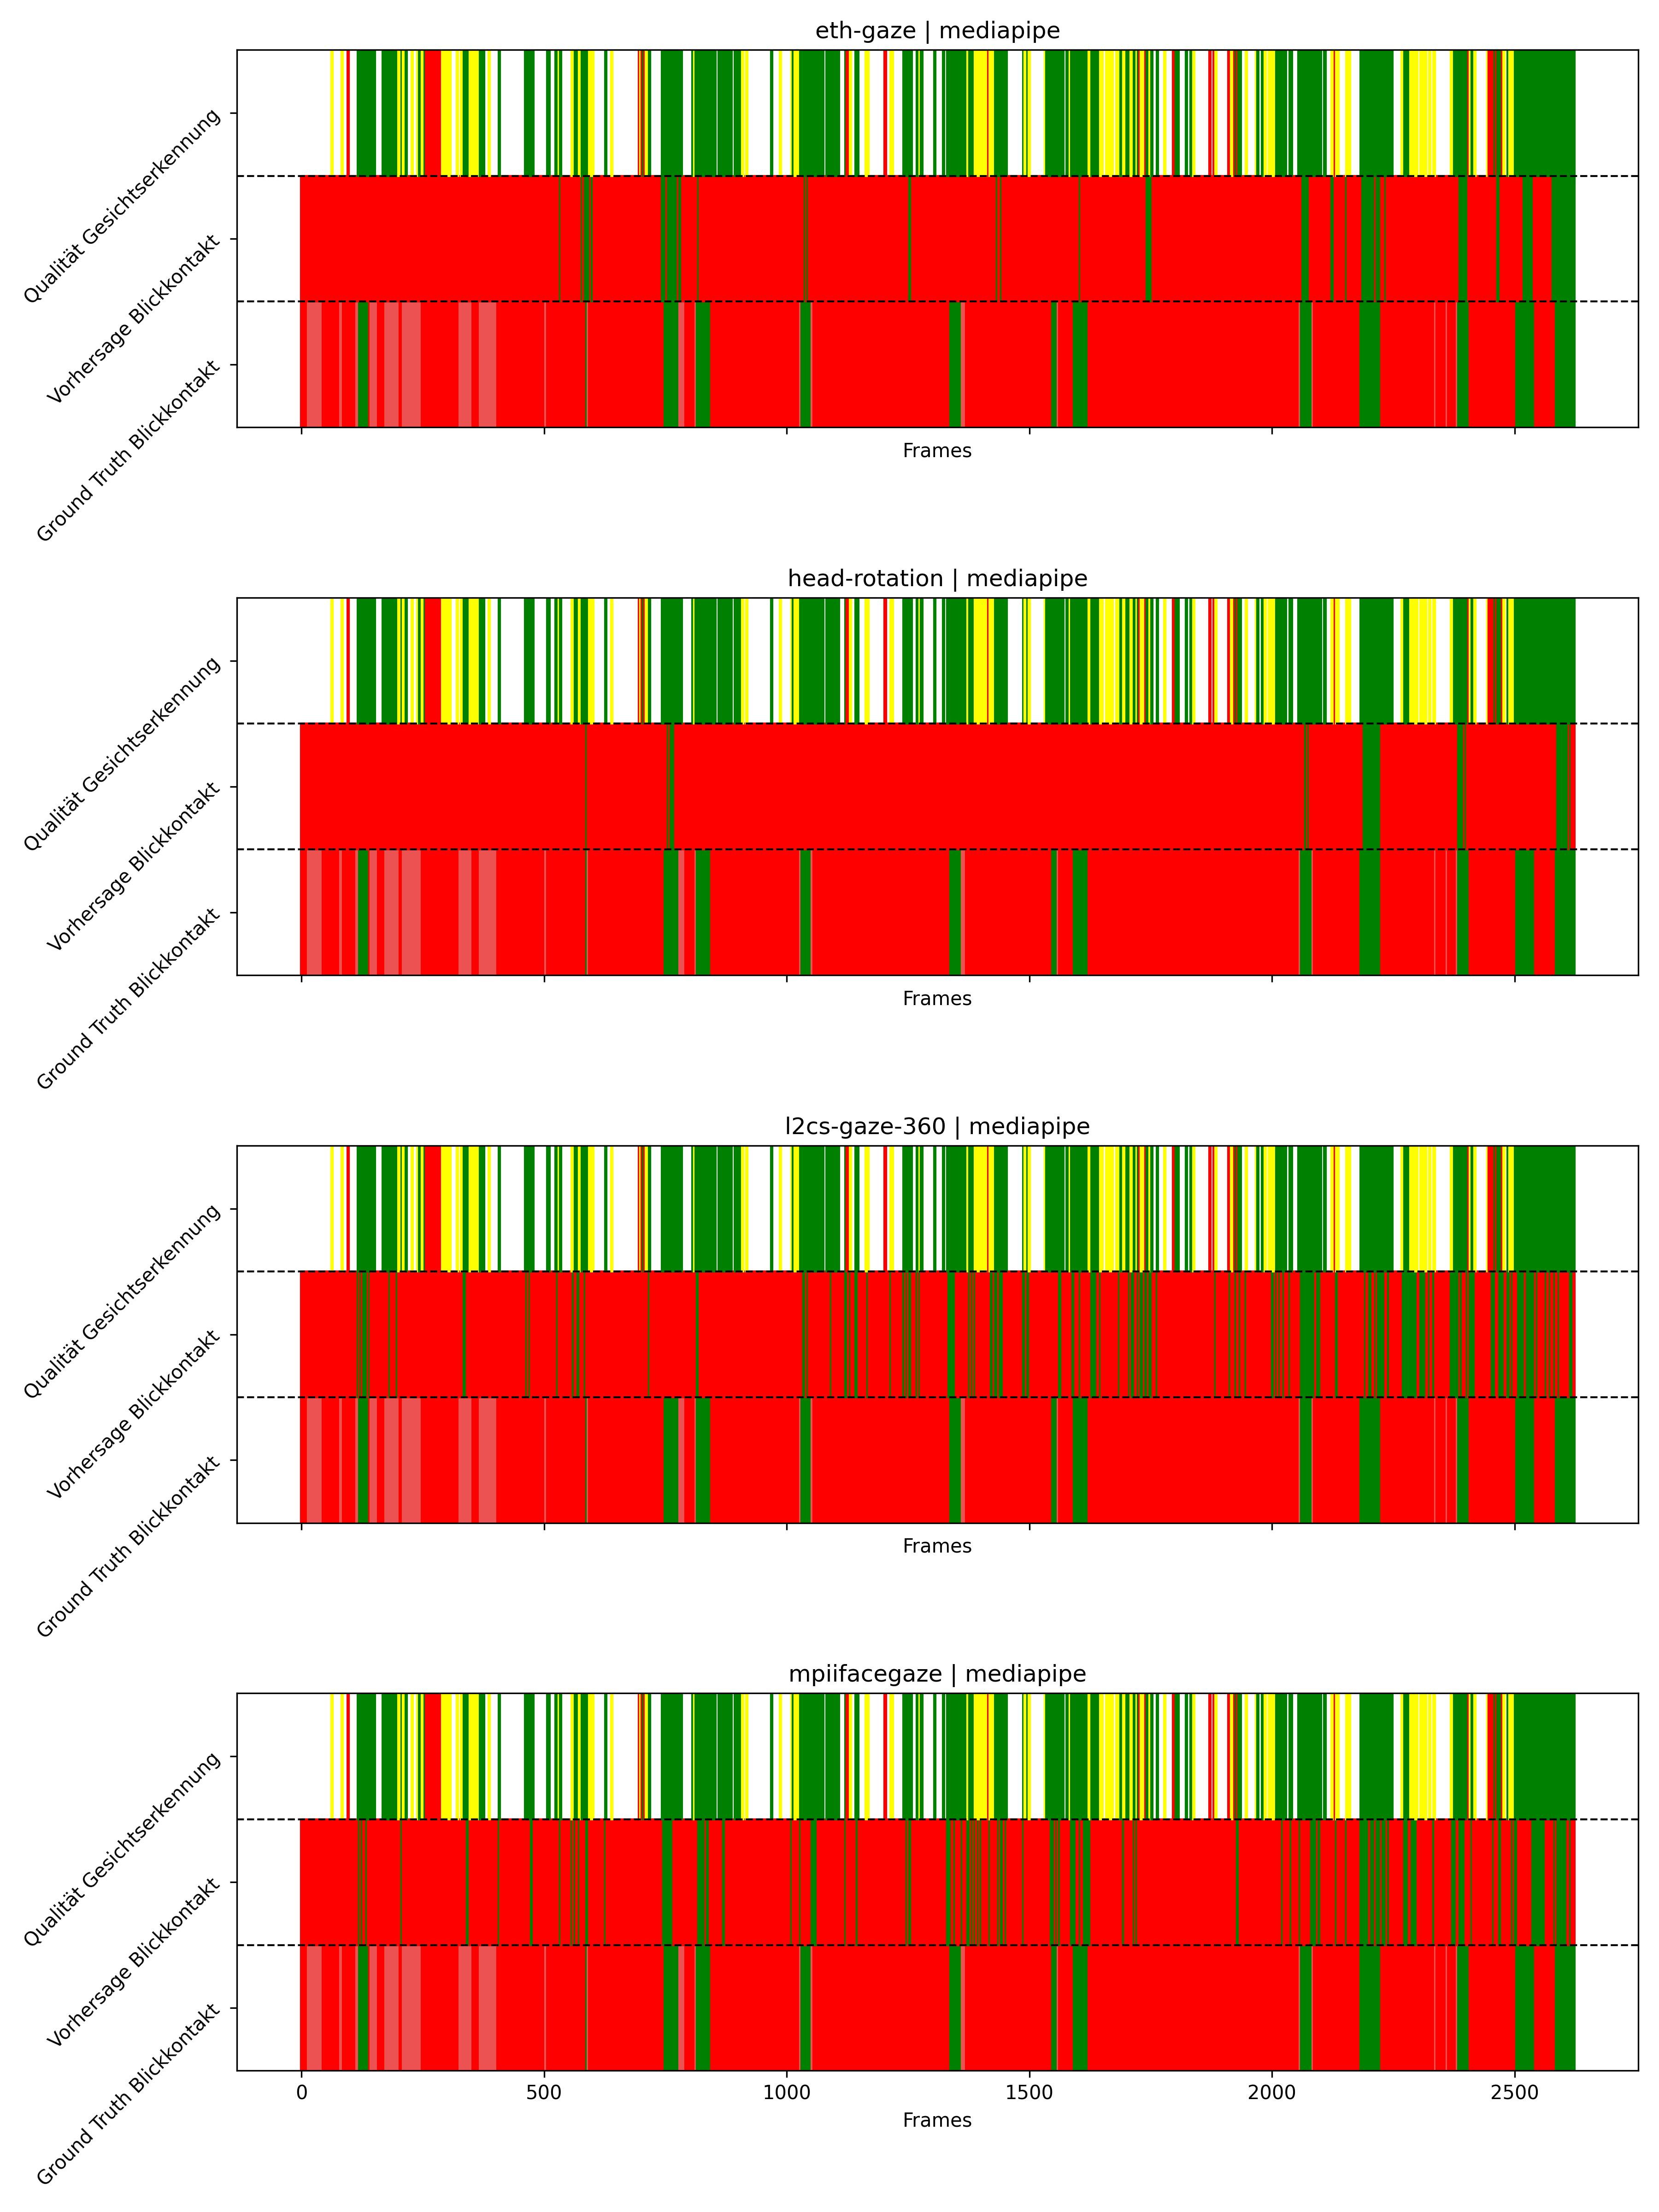
\includegraphics[width=1\linewidth]{appendix/07-mediapipe-overview-gaze.jpg}
\caption{Überblick über die Ground Truth des Blickkontakts, die Vorhersage des Blickkontakts und die Qualität der Gesichtserkennung mit \mediapipe. Die Bedeutung der Farben ist in Abbildung \ref{fig:evaluation:gaze:mpiifacegaze} erklärt.}
\end{figure}

\section{Video 08}
\begin{figure}[H]
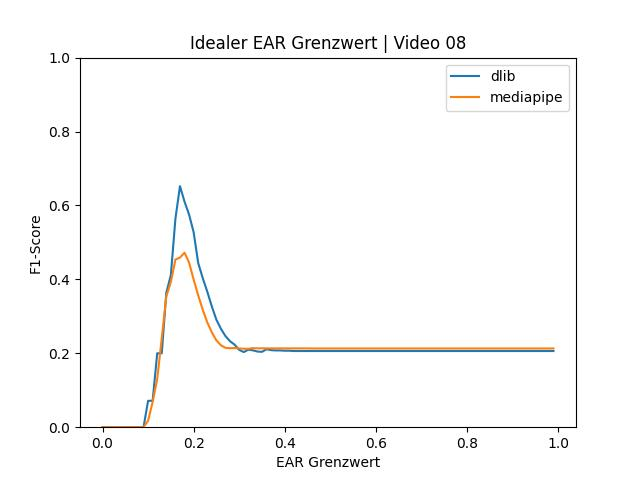
\includegraphics[width=0.7\linewidth]{appendix/08_f1-score-blink.jpg}
\caption{Ergebnisse der Bestimmung des idealen EAR-Grenzwerts für Video 08.}
\end{figure}

\begin{figure}[H]
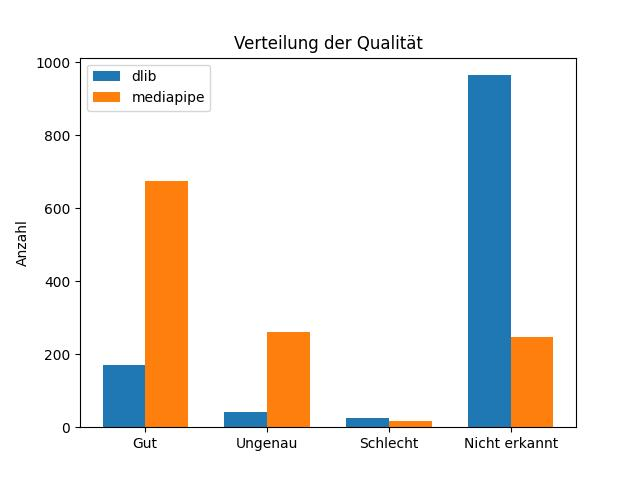
\includegraphics[width=0.7\linewidth]{appendix/08_bar-quality.jpg}
\caption{Aufteilung der Gesichtserkennungsqualität von Video 08.}
\end{figure}

\begin{table}[H]
\centering
\begin{tabular}{l|l|c c |c}
\toprule
\textbf{Gesichtserkennung} & \textbf{Blickrichtung} & \textbf{Seitenlänge} $\hitthresholdsize$ & \textbf{Verschiebung} $\hitthresholdposition$ & \textbf{F1-Score} \\ 
\midrule
\multirow{4}*{dlib}& ETH-XGaze & 0,133 & 0,084 & 0,722  \\ 
& Gaze360 & 0,398 & 0,108 & 0,704 \\ 
& MPIIFaceGaze & 0,041 & 0,01 & 0,516  \\ 
& Kopfrotation & 0,092 & 0,243 & 0,487  \\ 
\hline\multirow{4}*{MediaPipe}& ETH-XGaze & 0,224 & 0,047 & 0,835  \\ 
& Gaze360 & 0,398 & 0,108 & 0,847 \\ 
& MPIIFaceGaze & 0,041 & 0,022 & 0,52  \\ 
& Kopfrotation & 0,102 & 0,231 & 0,667  \\ 
\bottomrule\end{tabular}
\caption{Ergebnis des Hyperparameter-Tunings für die Zone speziell für Video 08.}
\label{tab:appendix:08:local}
\end{table}
\begin{table}[H]
\centering
\begin{tabular}{l|l|c c c c|c c|c}
\toprule
\textbf{Gesichtserkennung} & \textbf{Blickrichtung} & $TP$ & $TN$& $FP$ & $FN$ & \textbf{Precision} & \textbf{Recall} & \textbf{F1-Score} \\ 
\midrule
\multirow{4}*{dlib}& ETH-XGaze & 48 & 1108 & 3 & 39 & 0,941 & 0,552 & 0,696 \\ 
& Gaze360 & 32 & 1111 & 0 & 55 & 1,0 & 0,368 & 0,538 \\ 
& MPIIFaceGaze & 13 & 984 & 127 & 74 & 0,093 & 0,149 & 0,115 \\ 
& Kopfrotation & 28 & 1060 & 51 & 59 & 0,354 & 0,322 & 0,337 \\ 
\hline\multirow{4}*{MediaPipe}& ETH-XGaze & 45 & 1111 & 1 & 42 & 0,978 & 0,517 & 0,677 \\ 
& Gaze360 & 46 & 1110 & 2 & 41 & 0,958 & 0,529 & 0,681 \\ 
& MPIIFaceGaze & 12 & 608 & 504 & 75 & 0,023 & 0,138 & 0,04 \\ 
& Kopfrotation & 37 & 1101 & 11 & 50 & 0,771 & 0,425 & 0,548 \\ 
\bottomrule\end{tabular}
\caption{Zusammensetzung des F1-Scores unter Verwendung der in Kapitel \ref{sec:evaluation:results:gaze:threshold} bestimmten globalen Parameter $\hitthresholdsize$ und $\hitthresholdposition$.}
\label{tab:appendix:08:f1}
\end{table}
\begin{figure}[H]
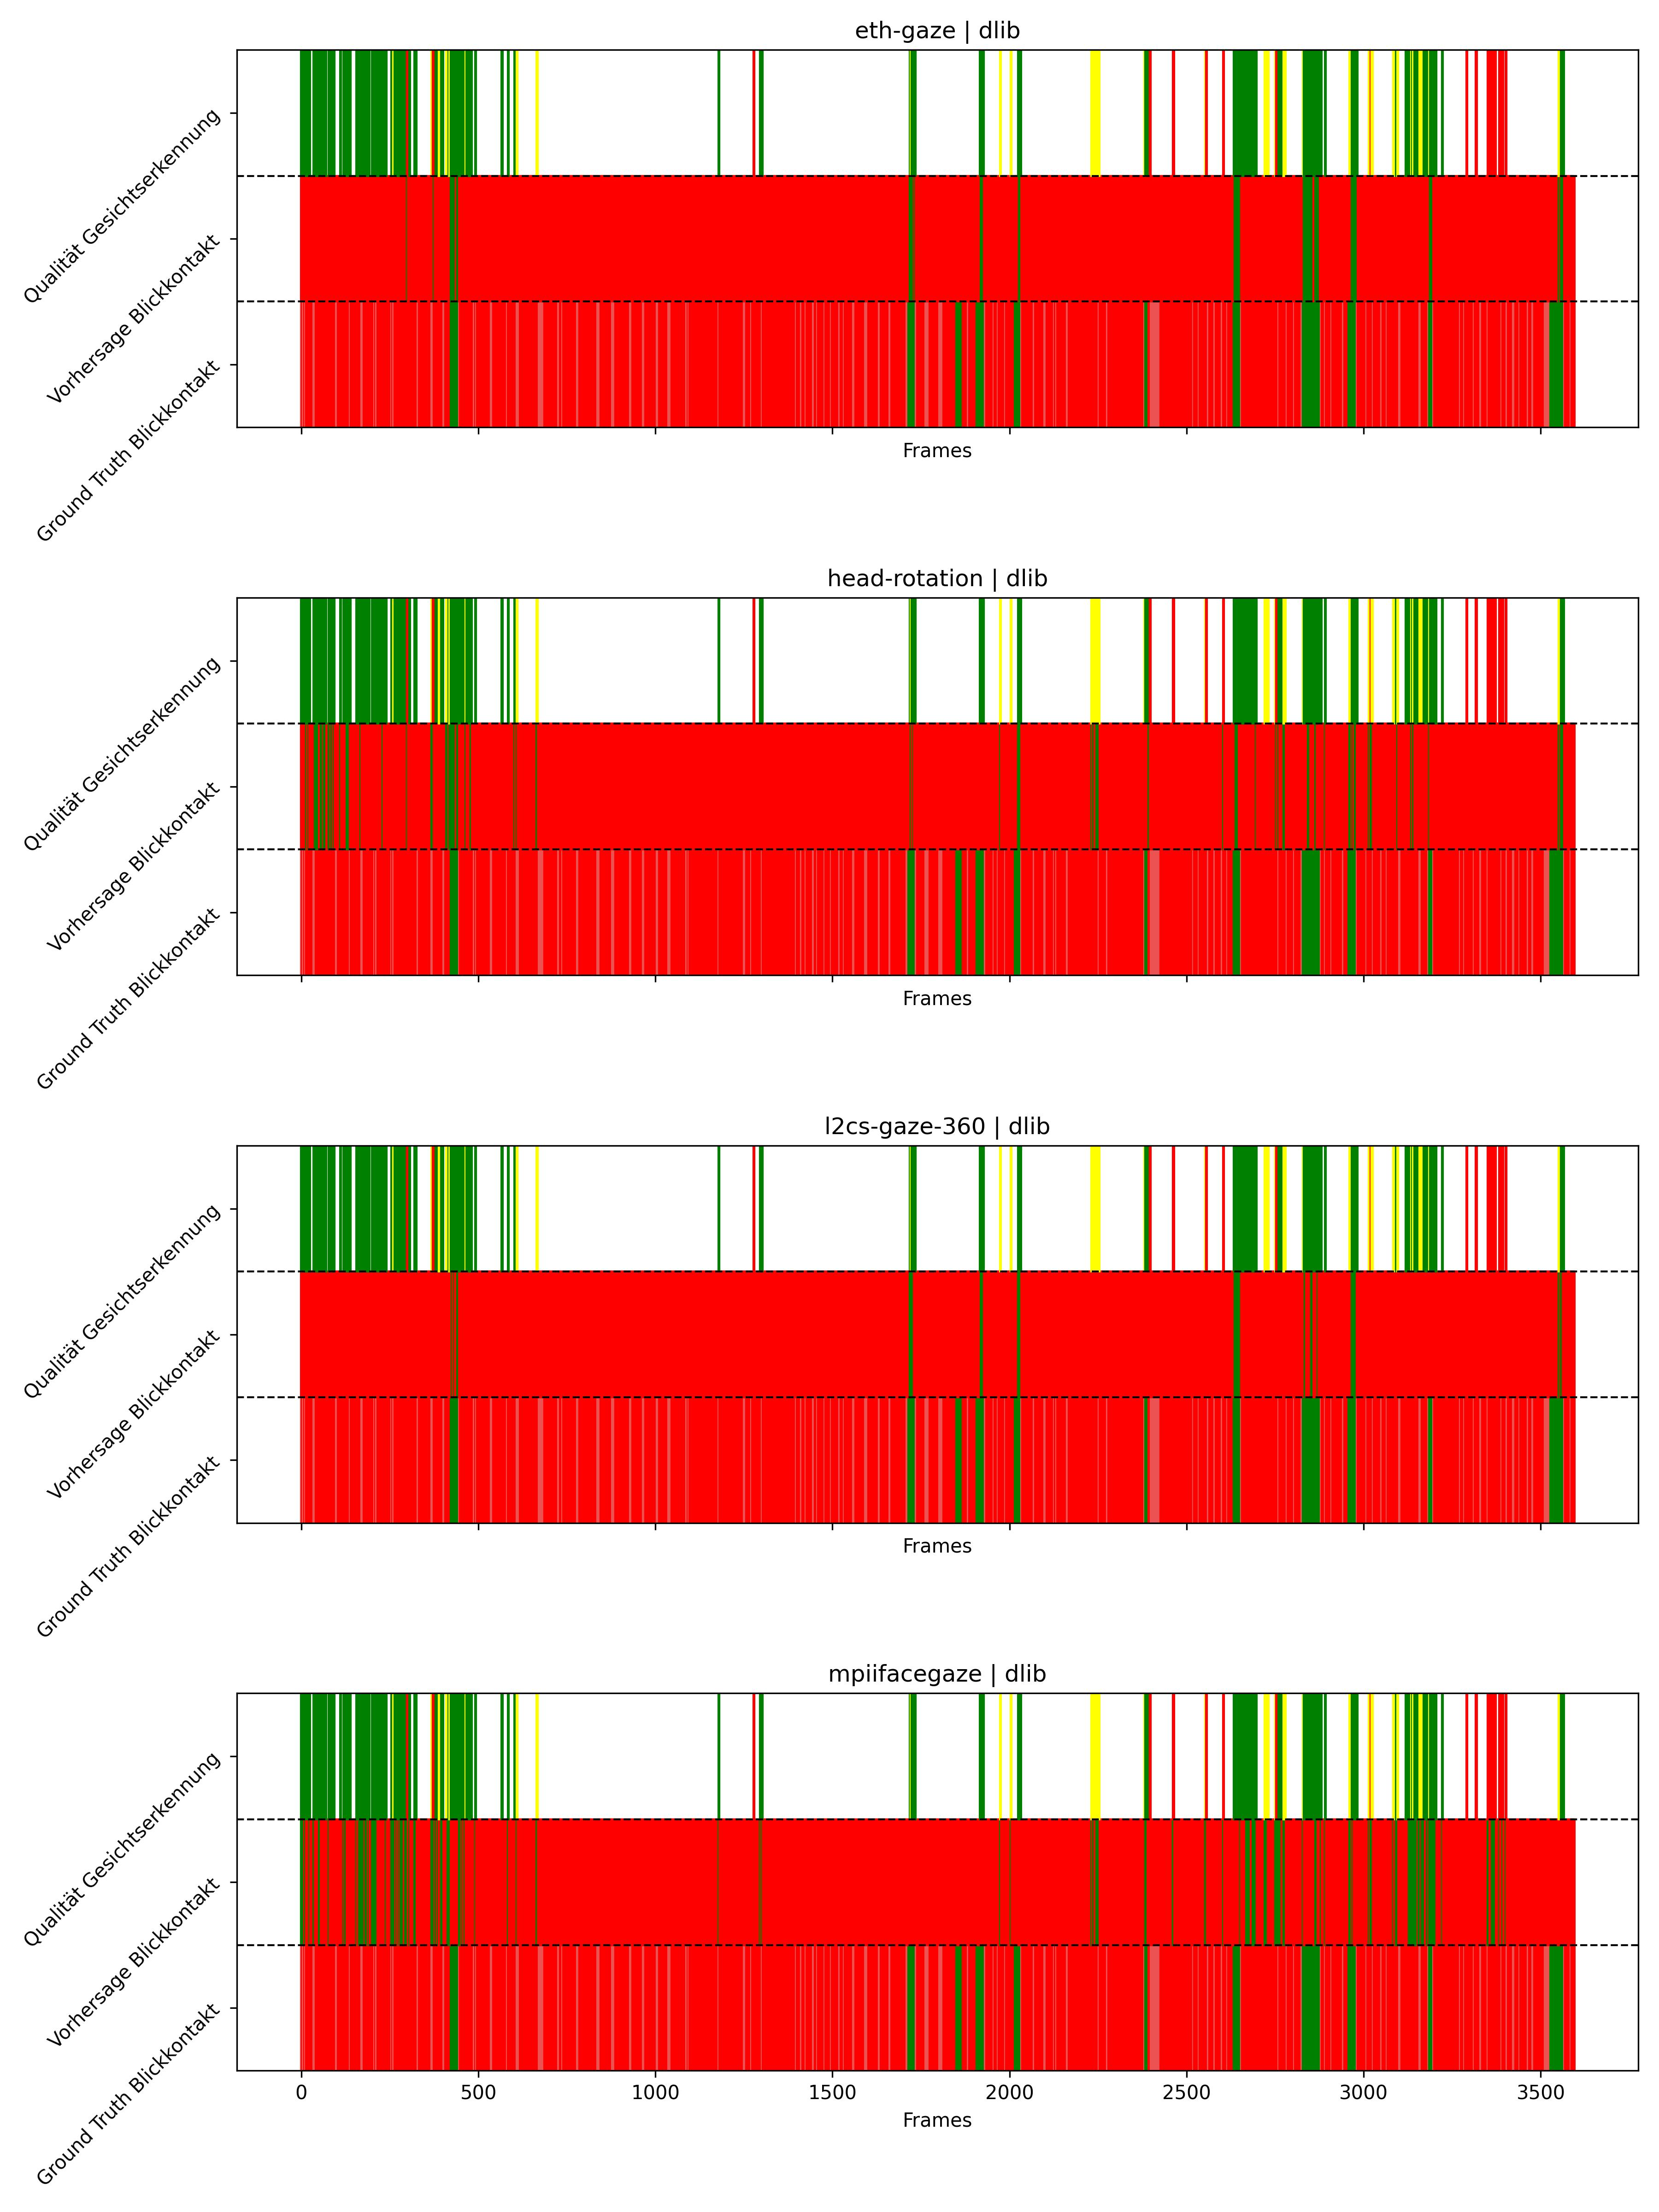
\includegraphics[width=1\linewidth]{appendix/08-dlib-overview-gaze.jpg}
\caption{Überblick über die Ground Truth des Blickkontakts, die Vorhersage des Blickkontakts und die Qualität der Gesichtserkennung mit \dlib. Die Bedeutung der Farben ist in Abbildung \ref{fig:evaluation:gaze:mpiifacegaze} erklärt.  }
\end{figure}

\begin{figure}[H]
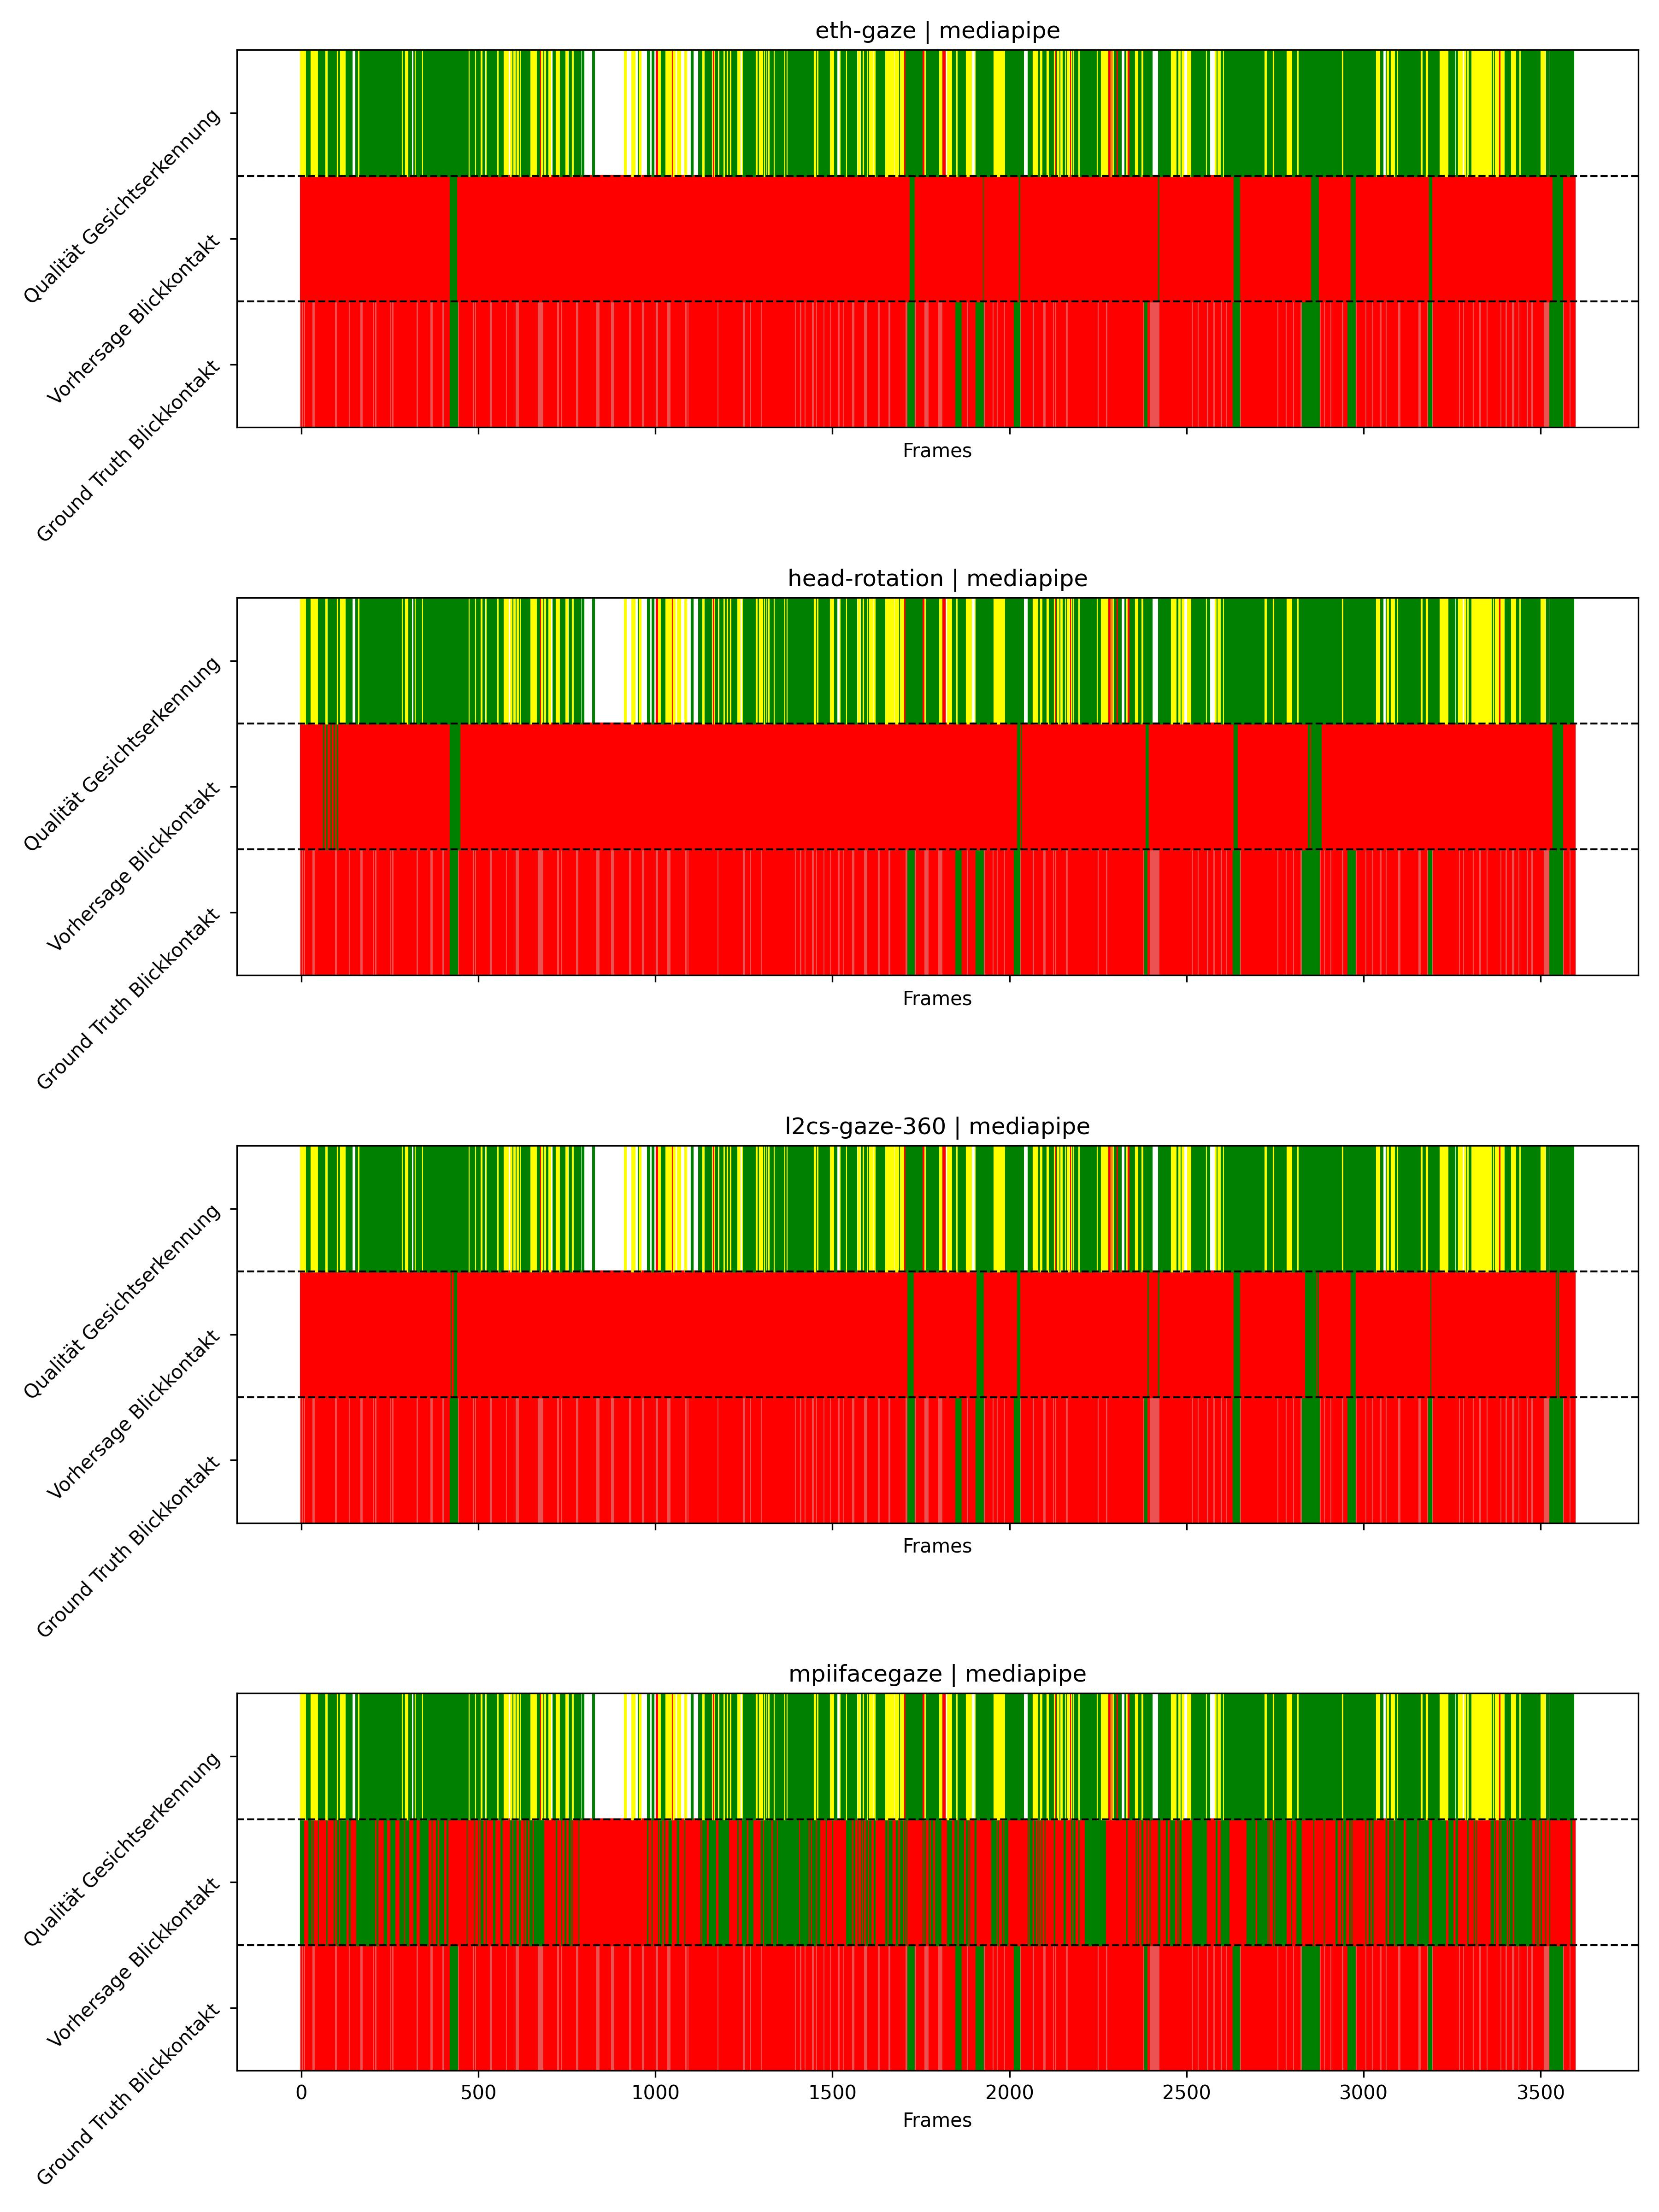
\includegraphics[width=1\linewidth]{appendix/08-mediapipe-overview-gaze.jpg}
\caption{Überblick über die Ground Truth des Blickkontakts, die Vorhersage des Blickkontakts und die Qualität der Gesichtserkennung mit \mediapipe. Die Bedeutung der Farben ist in Abbildung \ref{fig:evaluation:gaze:mpiifacegaze} erklärt.}
\end{figure}

\section{Video 09}\label{appendix:09}
\begin{figure}[H]
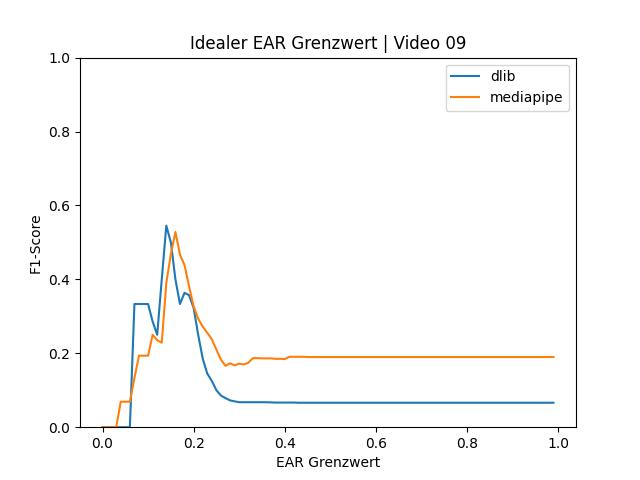
\includegraphics[width=0.7\linewidth]{appendix/09_f1-score-blink.jpg}
\caption{Ergebnisse der Bestimmung des idealen EAR-Grenzwerts für Video 09.}
\end{figure}

\begin{figure}[H]
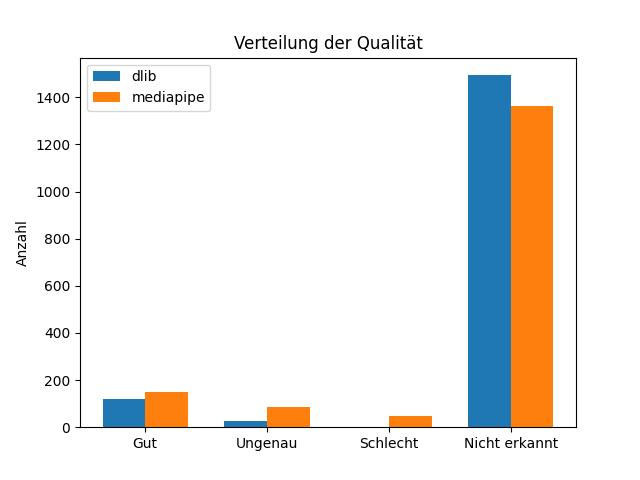
\includegraphics[width=0.7\linewidth]{appendix/09_bar-quality.jpg}
\caption{Aufteilung der Gesichtserkennungsqualität von Video 09.}
\end{figure}

\begin{table}[H]
\centering
\begin{tabular}{l|l|c c |c}
\toprule
\textbf{Gesichtserkennung} & \textbf{Blickrichtung} & \textbf{Seitenlänge} $\hitthresholdsize$ & \textbf{Verschiebung} $\hitthresholdposition$ & \textbf{F1-Score} \\ 
\midrule
\multirow{4}*{dlib}& ETH-XGaze & 0,163 & 0,047 & 0,949  \\ 
& Gaze360 & 0,214 & 0,084 & 0,949 \\ 
& MPIIFaceGaze & 0,051 & -0,039 & 0,939  \\ 
& Kopfrotation & 0,133 & 0,194 & 0,89  \\ 
\hline\multirow{4}*{MediaPipe}& ETH-XGaze & 0,143 & 0,022 & 0,882  \\ 
& Gaze360 & 0,459 & 0,047 & 0,963 \\ 
& MPIIFaceGaze & 0,051 & -0,027 & 0,724  \\ 
& Kopfrotation & 0,143 & 0,194 & 0,907  \\ 
\bottomrule\end{tabular}
\caption{Ergebnis des Hyperparameter-Tunings für die Zone speziell für Video 09.}
\label{tab:appendix:09:local}
\end{table}
\begin{table}[H]
\centering
\begin{tabular}{l|l|c c c c|c c|c}
\toprule
\textbf{Gesichtserkennung} & \textbf{Blickrichtung} & $TP$ & $TN$& $FP$ & $FN$ & \textbf{Precision} & \textbf{Recall} & \textbf{F1-Score} \\ 
\midrule
\multirow{4}*{dlib}& ETH-XGaze & 105 & 1514 & 7 & 14 & 0,938 & 0,882 & 0,909 \\ 
& Gaze360 & 113 & 1513 & 8 & 6 & 0,934 & 0,95 & 0,942 \\ 
& MPIIFaceGaze & 114 & 1503 & 18 & 5 & 0,864 & 0,958 & 0,908 \\ 
& Kopfrotation & 110 & 1499 & 22 & 9 & 0,833 & 0,924 & 0,876 \\ 
\hline\multirow{4}*{MediaPipe}& ETH-XGaze & 107 & 1490 & 32 & 12 & 0,77 & 0,899 & 0,829 \\ 
& Gaze360 & 116 & 1514 & 8 & 3 & 0,935 & 0,975 & 0,955 \\ 
& MPIIFaceGaze & 105 & 1456 & 66 & 14 & 0,614 & 0,882 & 0,724 \\ 
& Kopfrotation & 107 & 1505 & 17 & 12 & 0,863 & 0,899 & 0,881 \\ 
\bottomrule\end{tabular}
\caption{Zusammensetzung des F1-Scores unter Verwendung der in Kapitel \ref{sec:evaluation:results:gaze:threshold} bestimmten globalen Parameter $\hitthresholdsize$ und $\hitthresholdposition$.}
\label{tab:appendix:09:f1}
\end{table}
\begin{figure}[H]
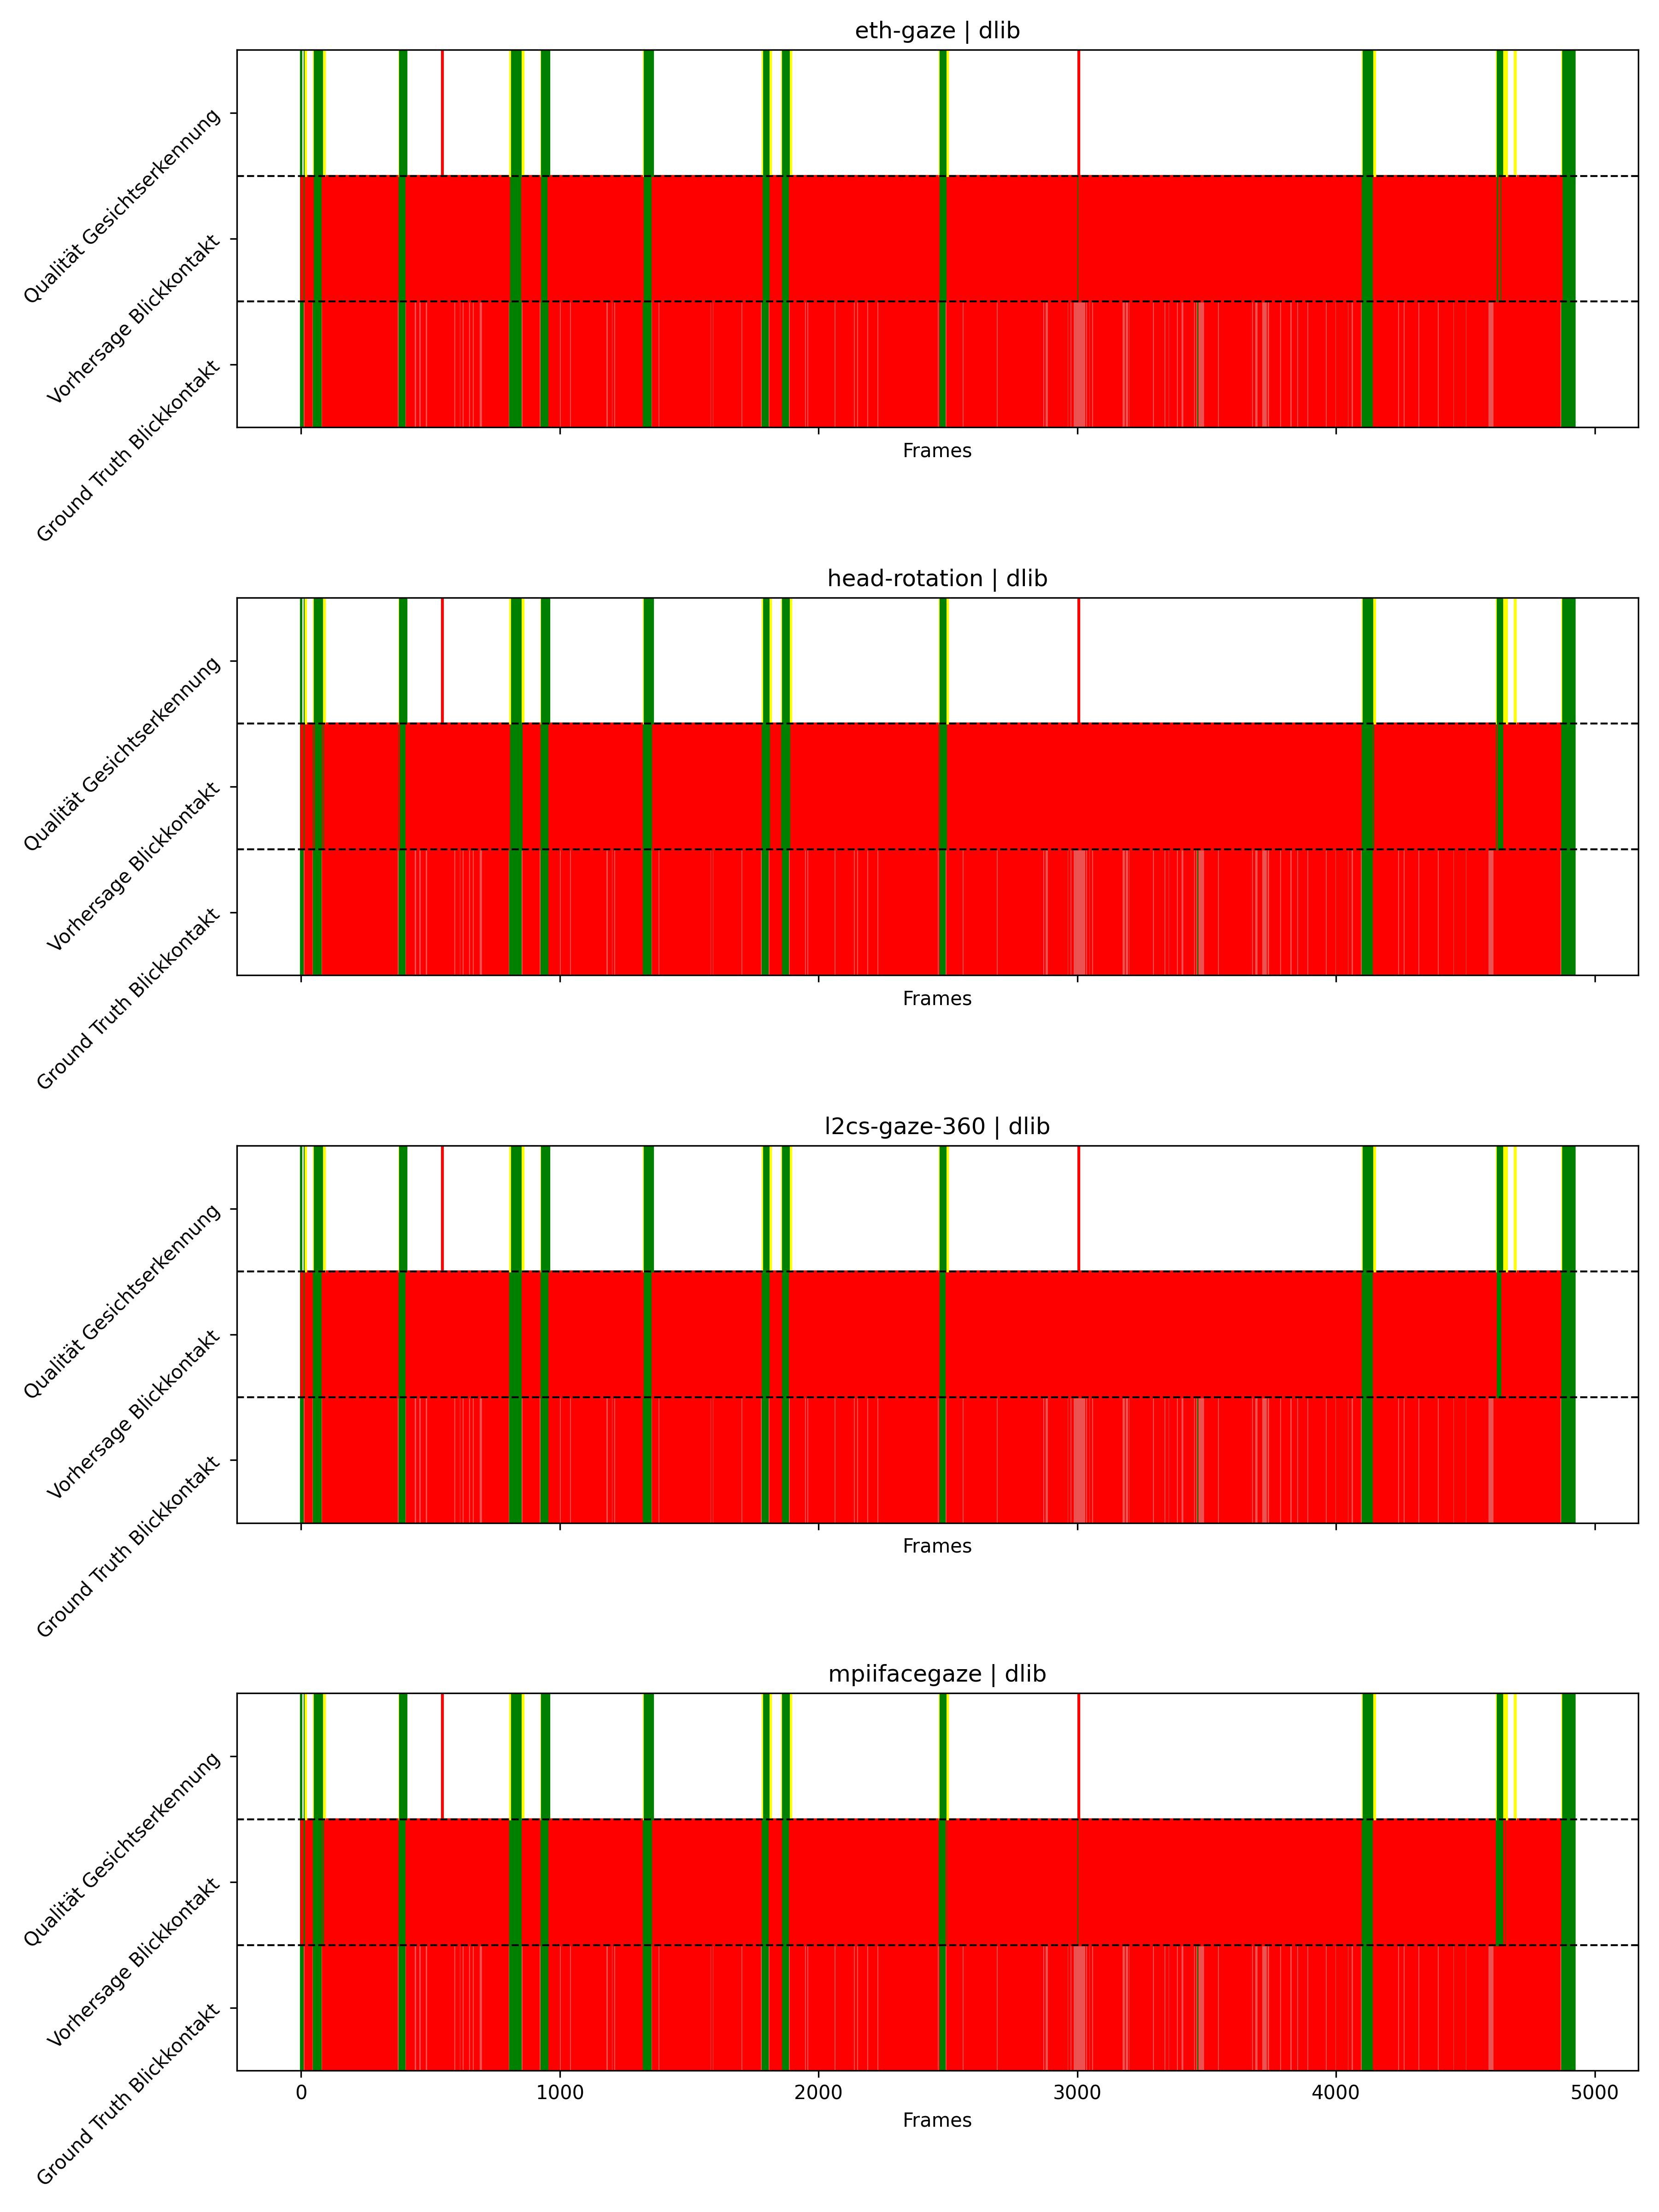
\includegraphics[width=1\linewidth]{appendix/09-dlib-overview-gaze.jpg}
\caption{Überblick über die Ground Truth des Blickkontakts, die Vorhersage des Blickkontakts und die Qualität der Gesichtserkennung mit \dlib. Die Bedeutung der Farben ist in Abbildung \ref{fig:evaluation:gaze:mpiifacegaze} erklärt.   }
\label{fig:appendix:09:dlib}
\end{figure}

\begin{figure}[H]
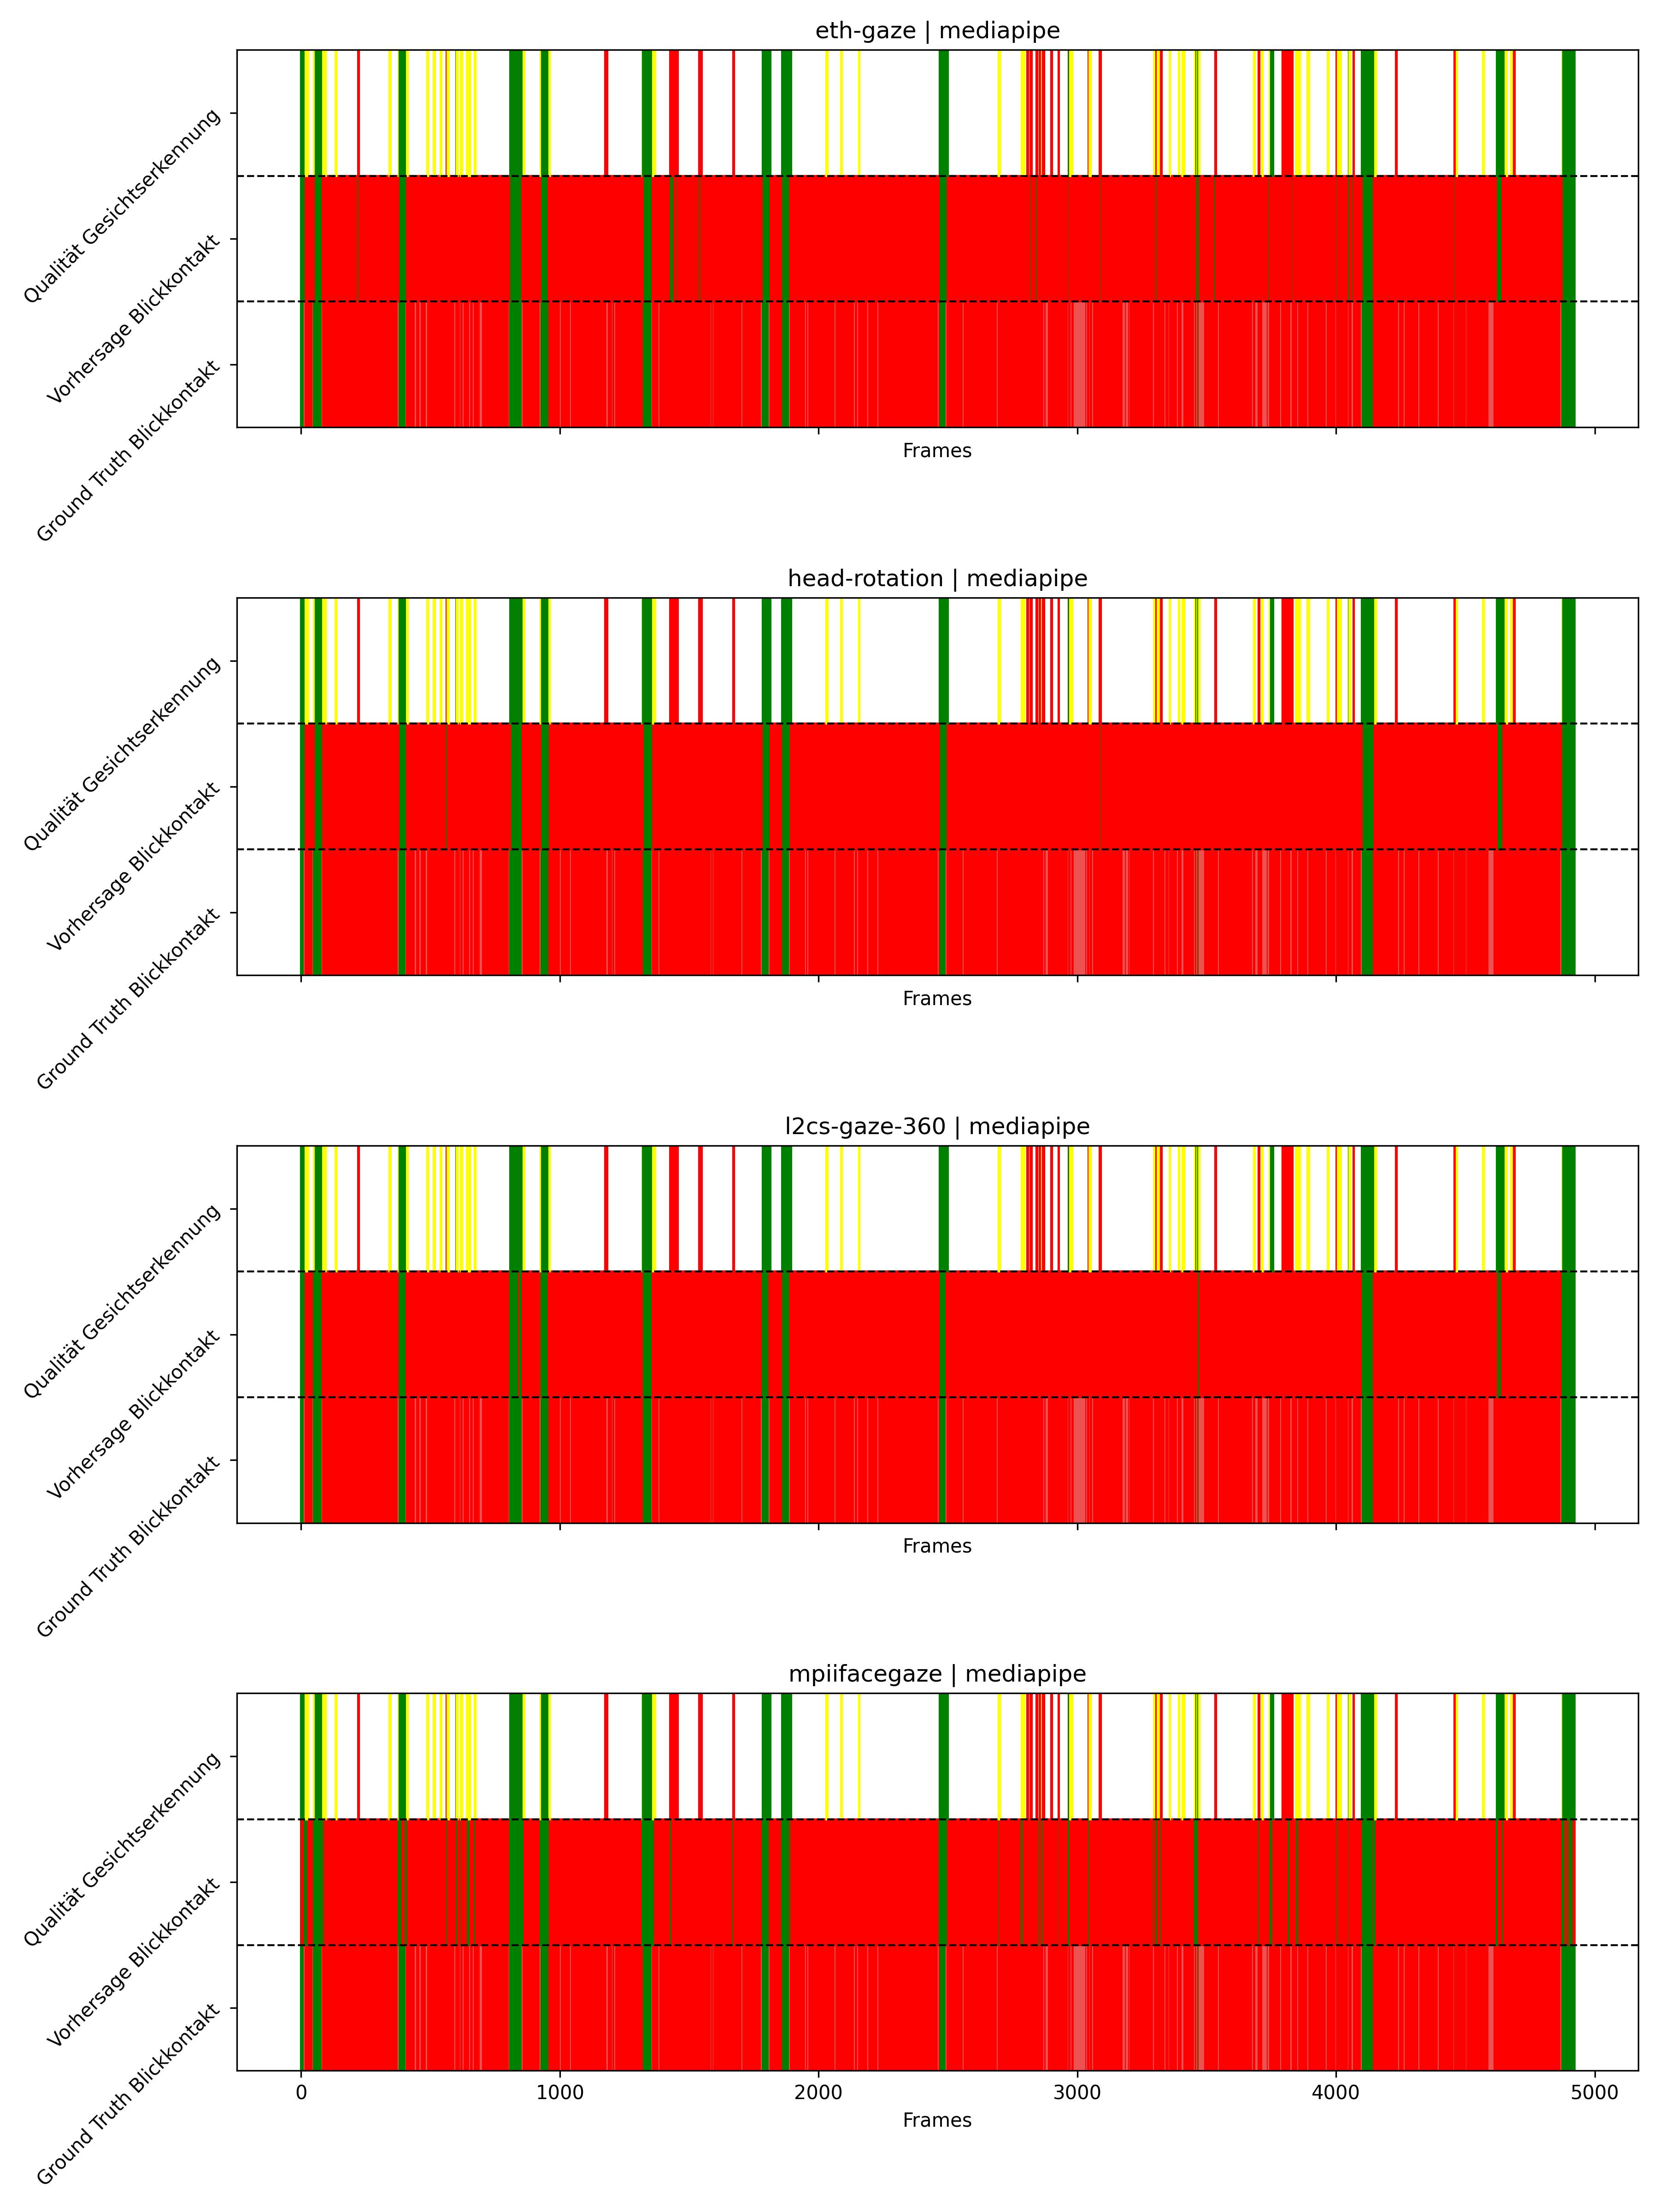
\includegraphics[width=1\linewidth]{appendix/09-mediapipe-overview-gaze.jpg}
\caption{Überblick über die Ground Truth des Blickkontakts, die Vorhersage des Blickkontakts und die Qualität der Gesichtserkennung mit \mediapipe. Die Bedeutung der Farben ist in Abbildung \ref{fig:evaluation:gaze:mpiifacegaze} erklärt.}
\label{fig:appendix:09:mediapipe}
\end{figure}

\section{Video 10}
\begin{figure}[H]
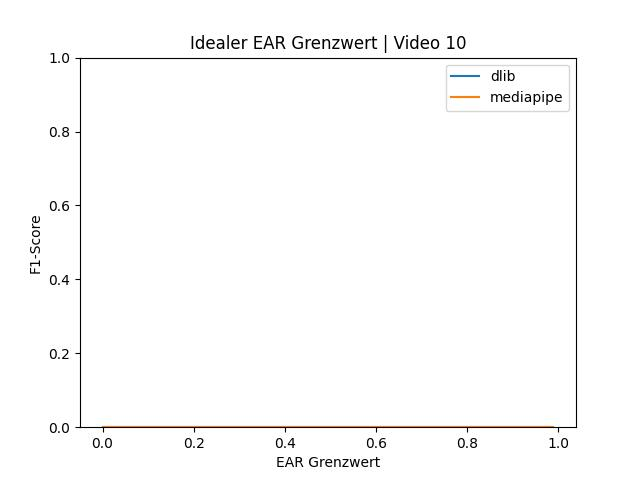
\includegraphics[width=0.7\linewidth]{appendix/10_f1-score-blink.jpg}
\caption{Ergebnisse der Bestimmung des idealen EAR-Grenzwerts für Video 10. Durch die Sonnenbrille von \philipp waren die Augen in keinem der Bilder zu sehen.}
\end{figure}

\begin{figure}[H]
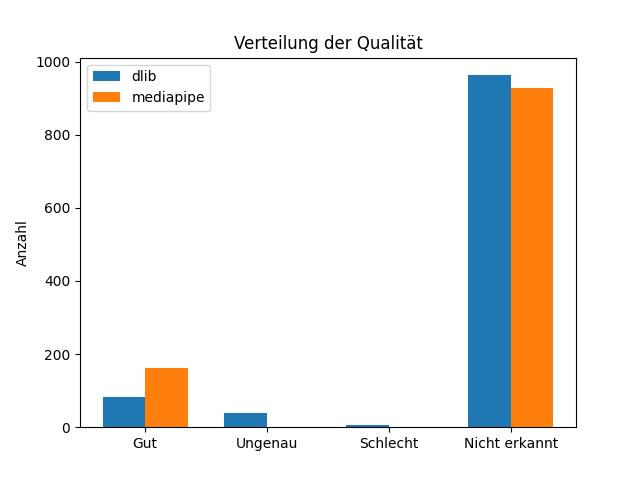
\includegraphics[width=0.7\linewidth]{appendix/10_bar-quality.jpg}
\caption{Aufteilung der Gesichtserkennungsqualität von Video 10.}
\end{figure}

\begin{table}[H]
\centering
\begin{tabular}{l|l|c c |c}
\toprule
\textbf{Gesichtserkennung} & \textbf{Blickrichtung} & \textbf{Seitenlänge} $\hitthresholdsize$ & \textbf{Verschiebung} $\hitthresholdposition$ & \textbf{F1-Score} \\ 
\midrule
\multirow{4}*{dlib}& ETH-XGaze & 0,276 & 0,133 & 0,891  \\ 
& Gaze360 & 0,49 & 0,145 & 0,63 \\ 
& MPIIFaceGaze & 0,092 & 0,022 & 0,891  \\ 
& Kopfrotation & 0,265 & 0,218 & 0,891  \\ 
\hline\multirow{4}*{MediaPipe}& ETH-XGaze & 0,245 & 0,133 & 0,963  \\ 
& Gaze360 & 0,5 & 0,133 & 0,667 \\ 
& MPIIFaceGaze & 0,092 & 0,022 & 0,952  \\ 
& Kopfrotation & 0,214 & 0,255 & 0,977  \\ 
\bottomrule\end{tabular}
\caption{Ergebnis des Hyperparameter-Tunings für die Zone speziell für Video 10.}
\label{tab:appendix:10:local}
\end{table}
\begin{table}[H]
\centering
\begin{tabular}{l|l|c c c c|c c|c}
\toprule
\textbf{Gesichtserkennung} & \textbf{Blickrichtung} & $TP$ & $TN$& $FP$ & $FN$ & \textbf{Precision} & \textbf{Recall} & \textbf{F1-Score} \\ 
\midrule
\multirow{4}*{dlib}& ETH-XGaze & 71 & 941 & 1 & 77 & 0,986 & 0,48 & 0,645 \\ 
& Gaze360 & 47 & 942 & 0 & 101 & 1,0 & 0,318 & 0,482 \\ 
& MPIIFaceGaze & 40 & 942 & 0 & 108 & 1,0 & 0,27 & 0,426 \\ 
& Kopfrotation & 121 & 938 & 4 & 27 & 0,968 & 0,818 & 0,886 \\ 
\hline\multirow{4}*{MediaPipe}& ETH-XGaze & 64 & 942 & 0 & 84 & 1,0 & 0,432 & 0,604 \\ 
& Gaze360 & 45 & 942 & 0 & 103 & 1,0 & 0,304 & 0,466 \\ 
& MPIIFaceGaze & 52 & 931 & 11 & 96 & 0,825 & 0,351 & 0,493 \\ 
& Kopfrotation & 130 & 942 & 0 & 18 & 1,0 & 0,878 & 0,935 \\ 
\bottomrule\end{tabular}
\caption{Zusammensetzung des F1-Scores unter Verwendung der in Kapitel \ref{sec:evaluation:results:gaze:threshold} bestimmten globalen Parameter $\hitthresholdsize$ und $\hitthresholdposition$.}
\label{tab:appendix:10:f1}
\end{table}

\begin{figure}[H]
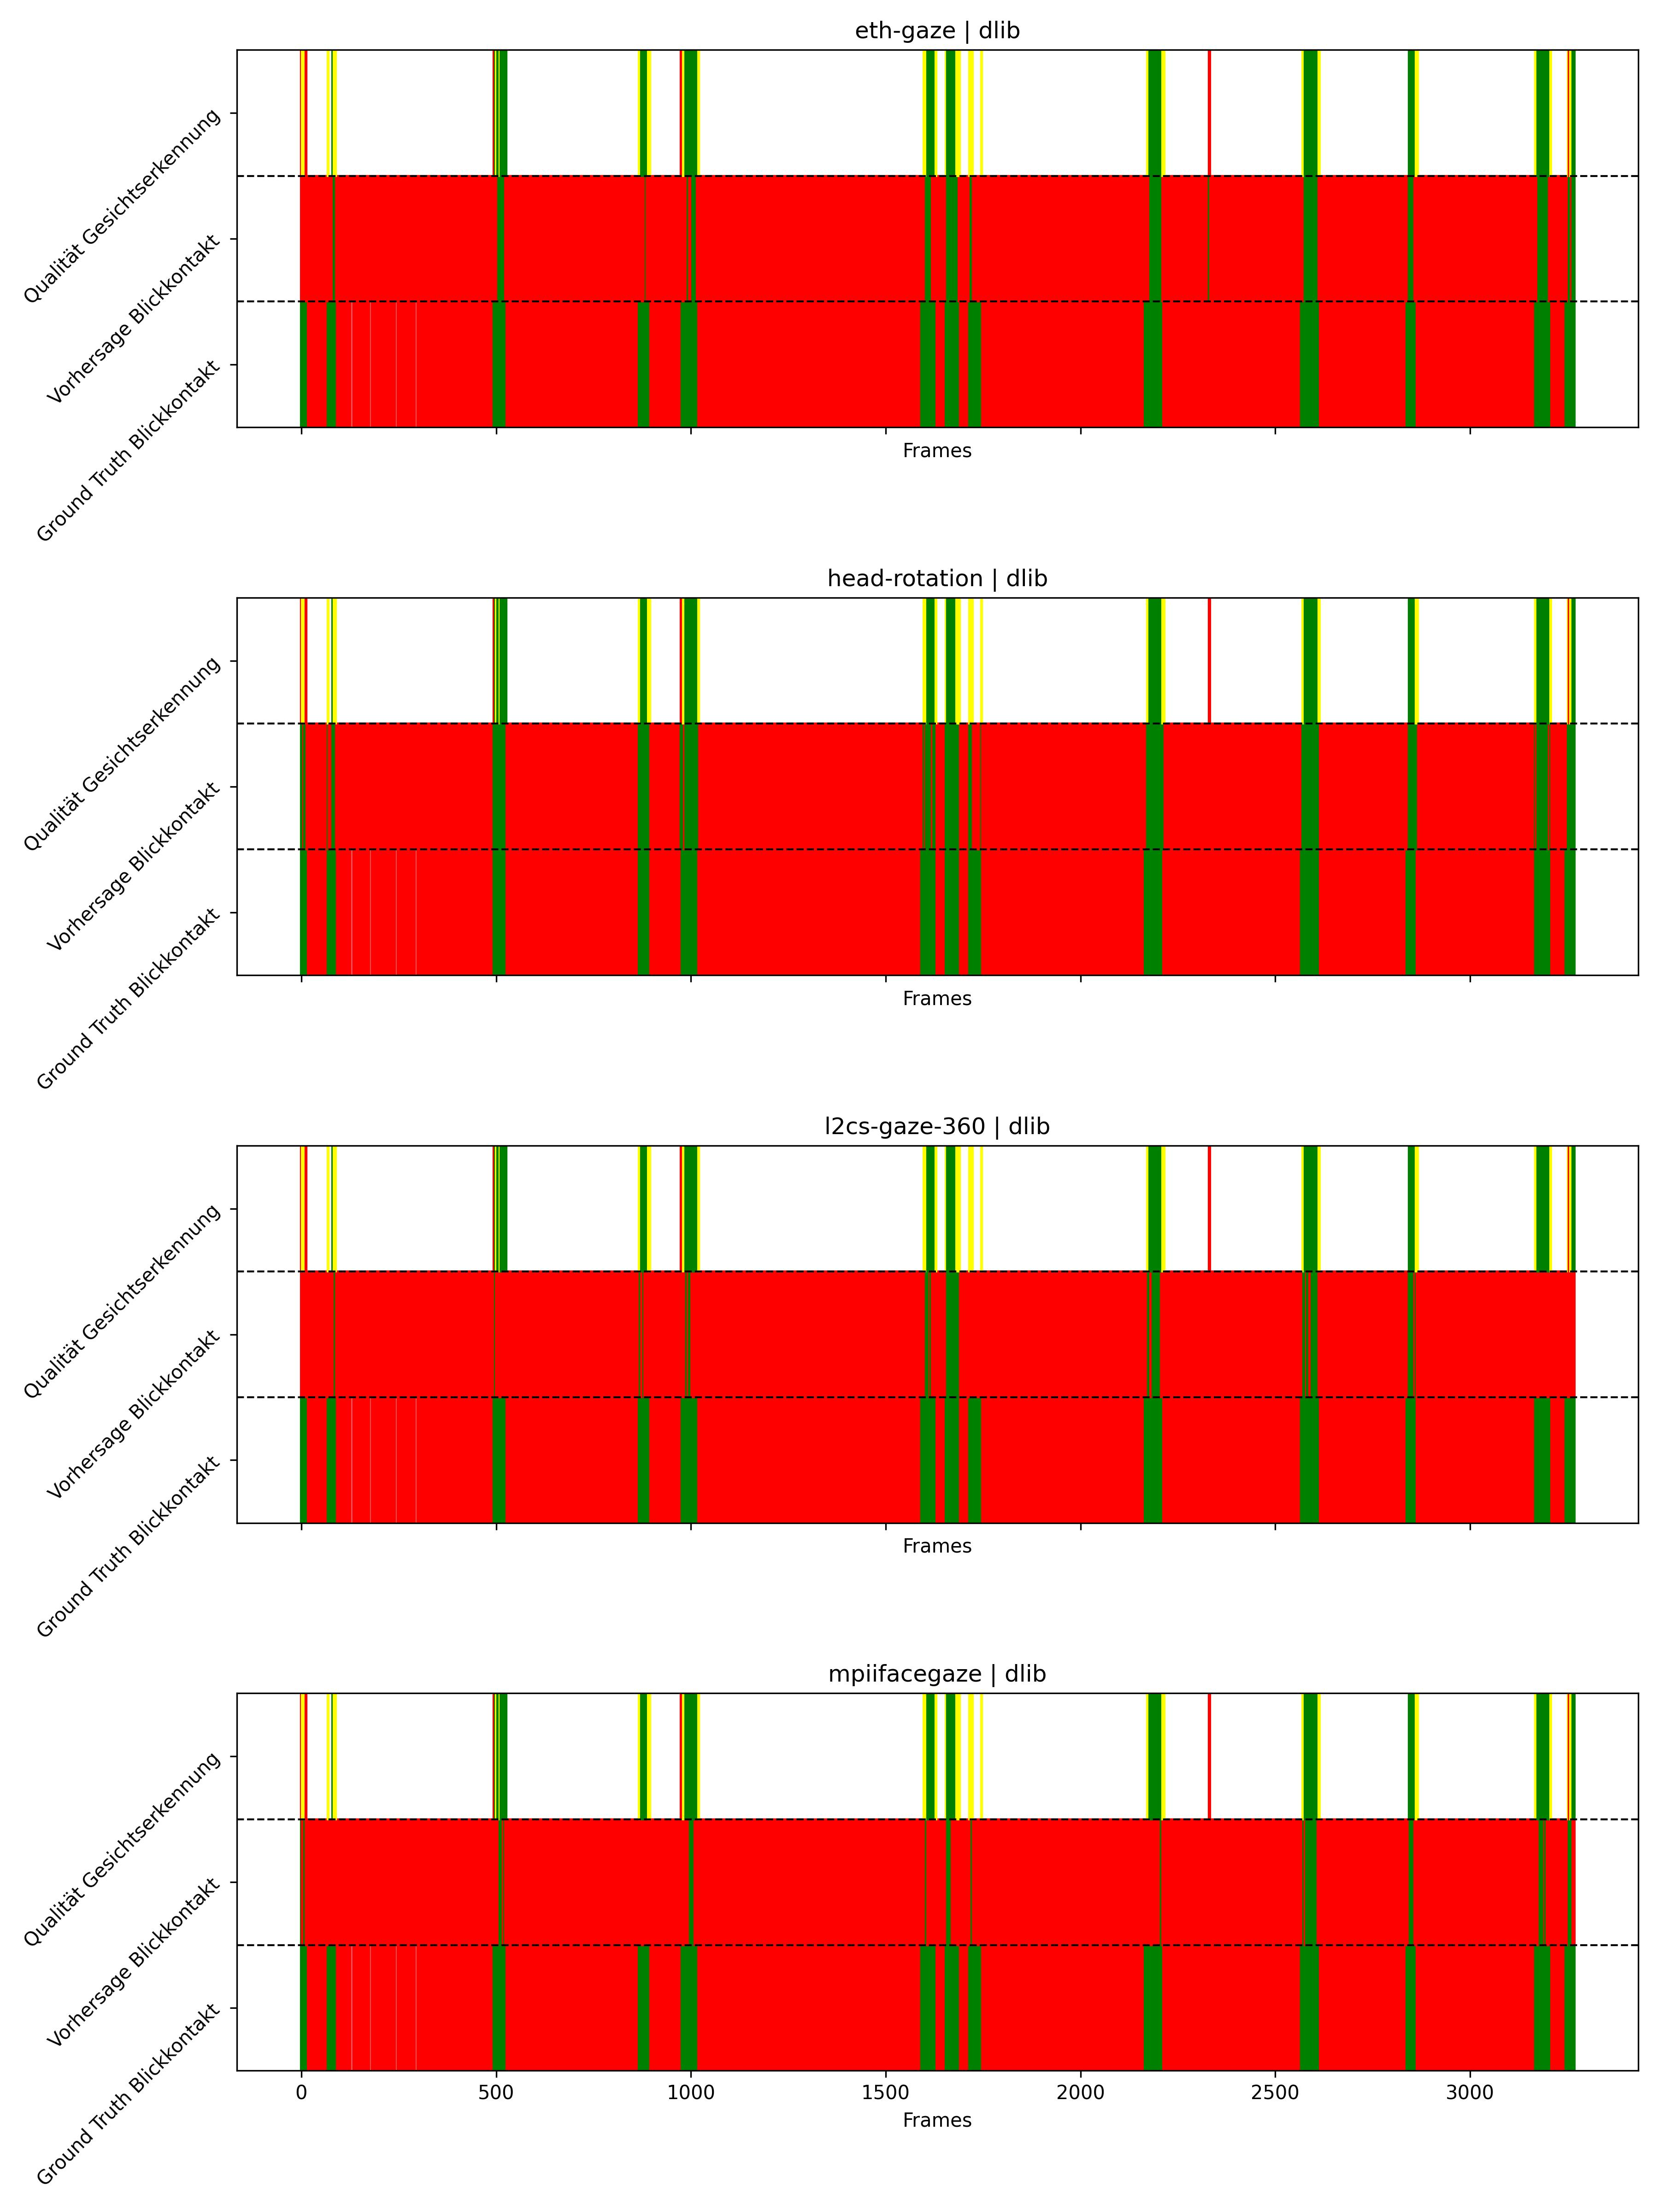
\includegraphics[width=1\linewidth]{appendix/10-dlib-overview-gaze.jpg}
\caption{Überblick über die Ground Truth des Blickkontakts, die Vorhersage des Blickkontakts und die Qualität der Gesichtserkennung mit \dlib. Die Bedeutung der Farben ist in Abbildung \ref{fig:evaluation:gaze:mpiifacegaze} erklärt.   }
\end{figure}

\begin{figure}[H]
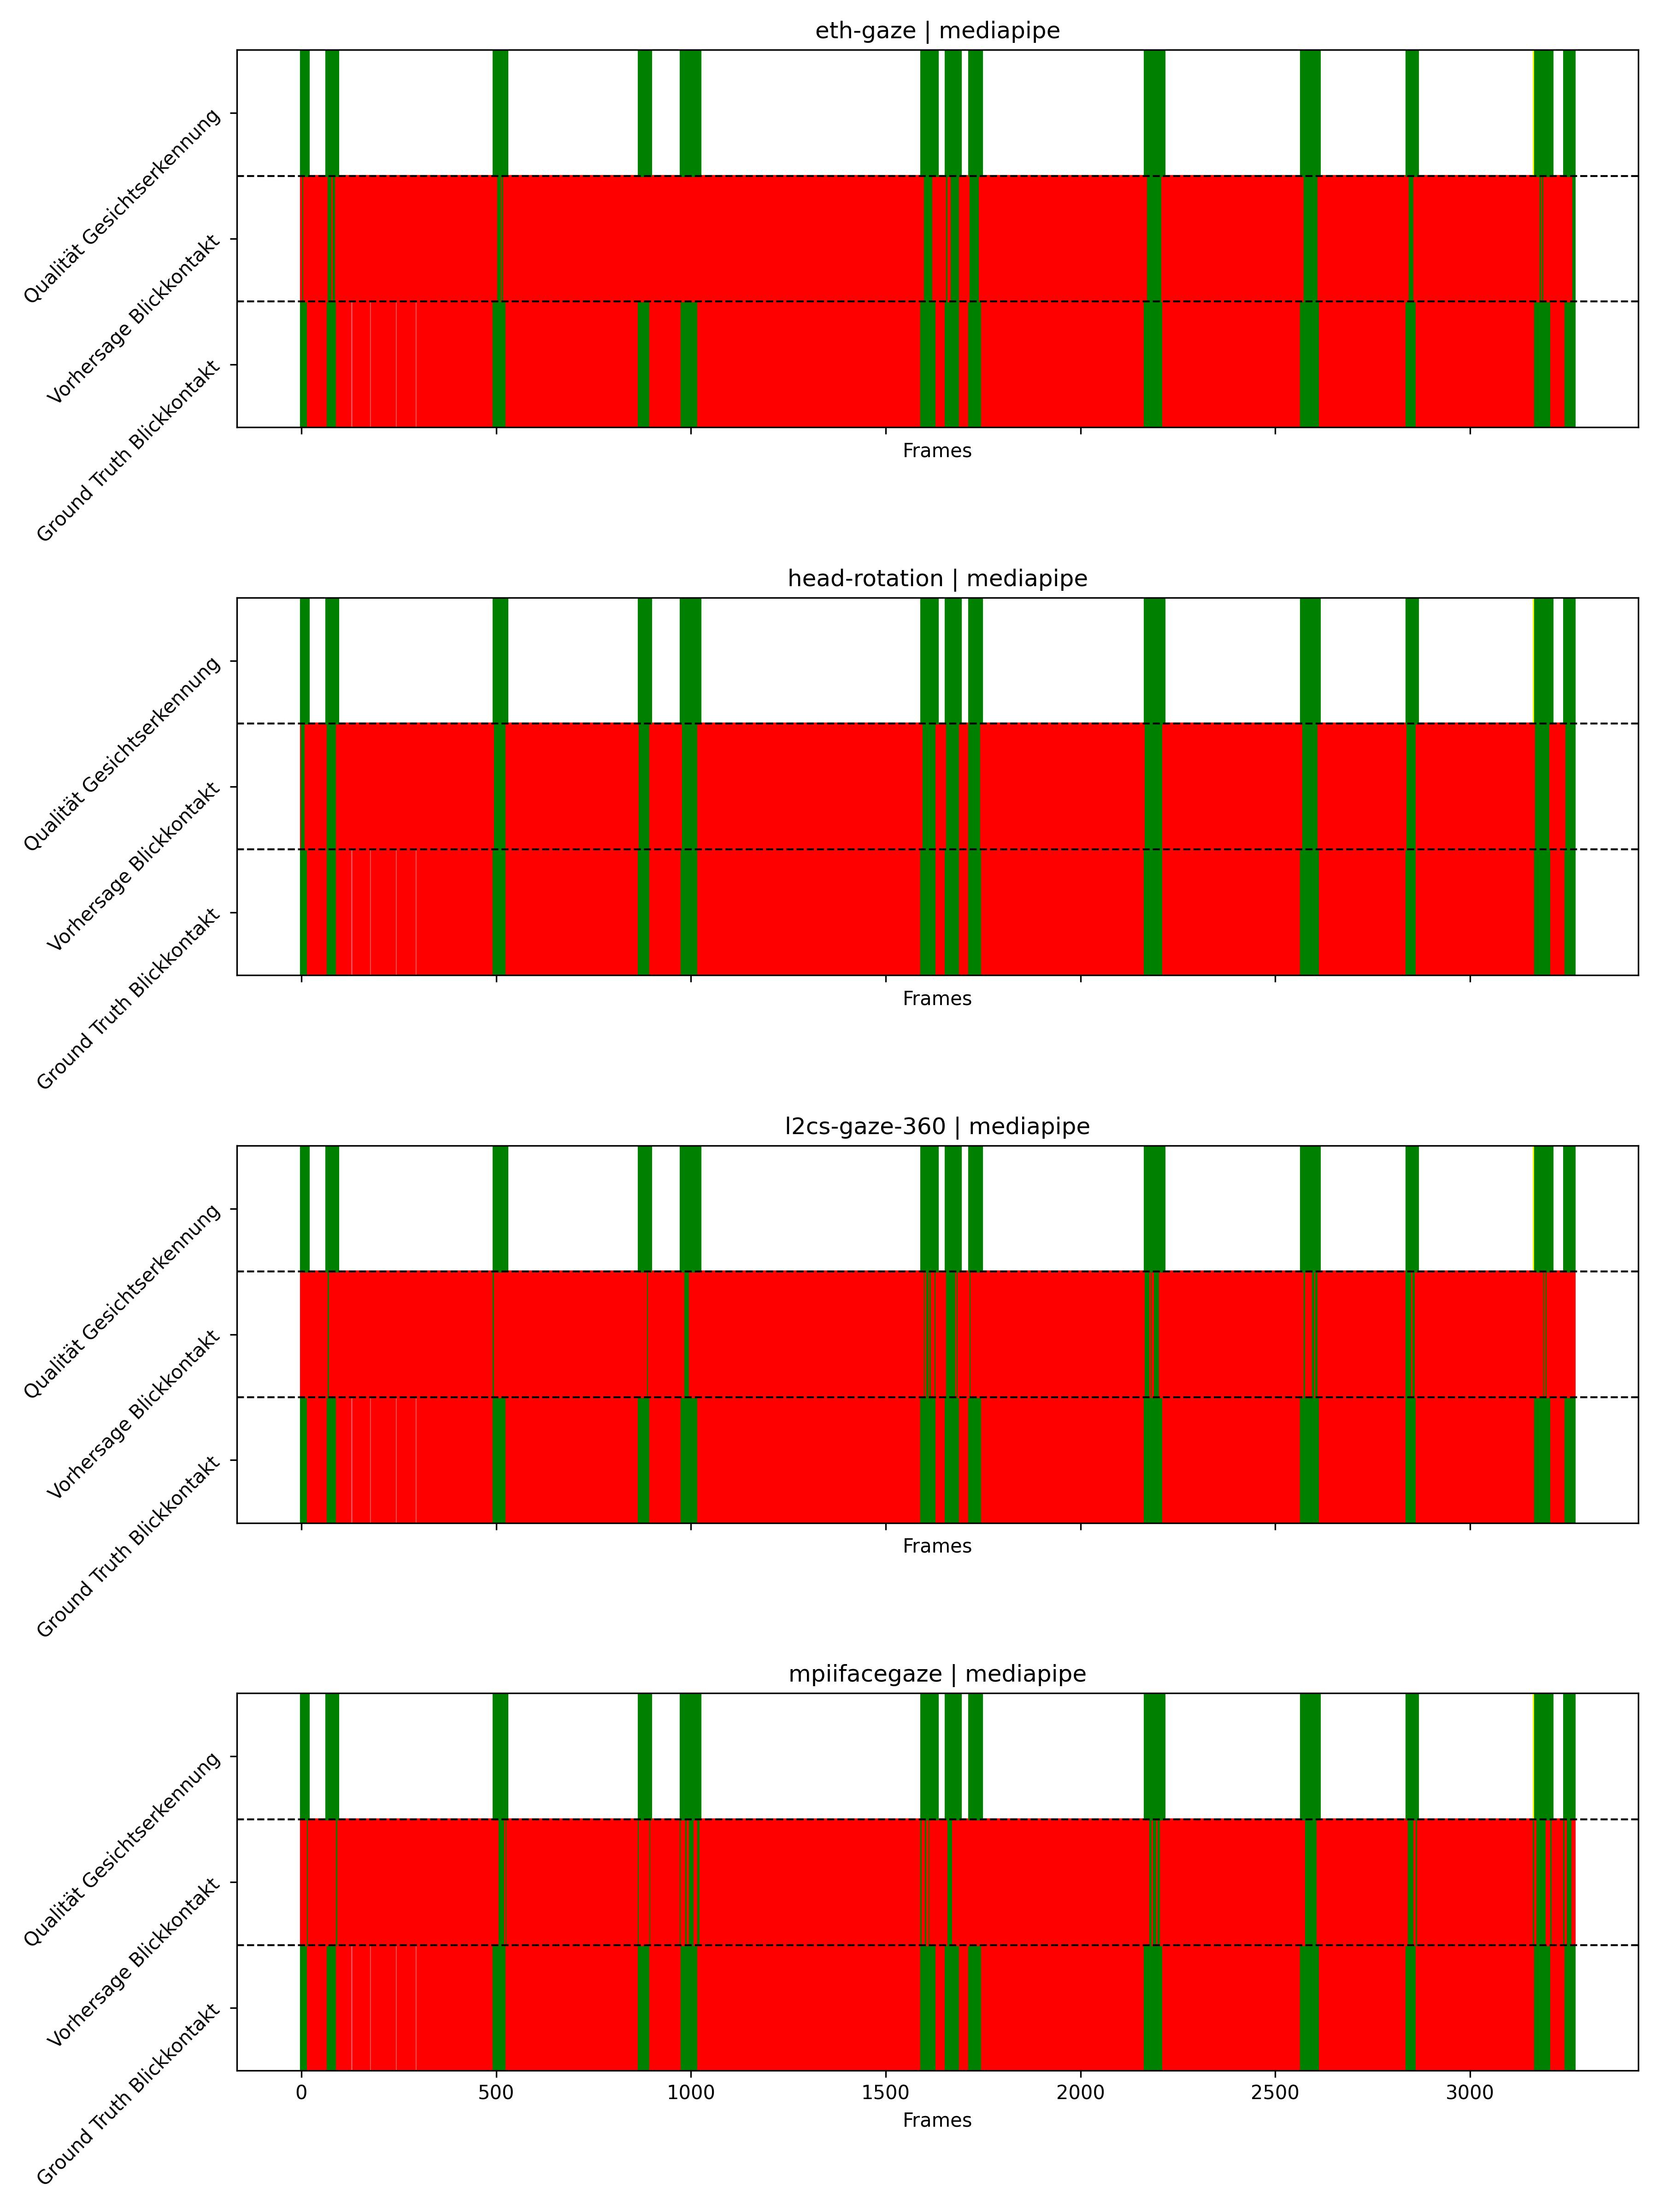
\includegraphics[width=1\linewidth]{appendix/10-mediapipe-overview-gaze.jpg}
\caption{Überblick über die Ground Truth des Blickkontakts, die Vorhersage des Blickkontakts und die Qualität der Gesichtserkennung mit \mediapipe. Die Bedeutung der Farben ist in Abbildung \ref{fig:evaluation:gaze:mpiifacegaze} erklärt.}
\end{figure}

\section{Video 11}
\begin{figure}[H]
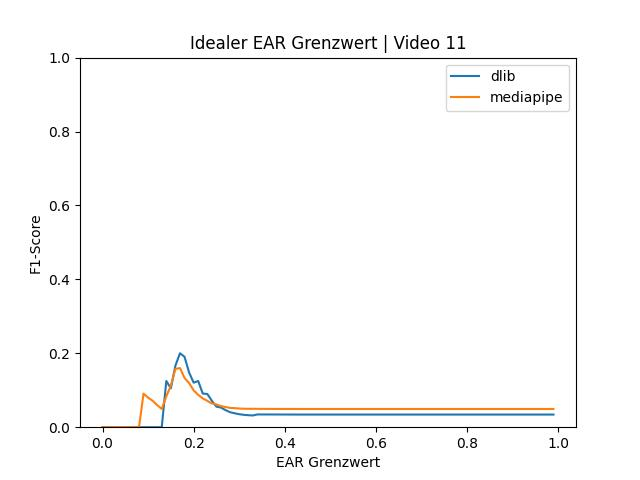
\includegraphics[width=0.7\linewidth]{appendix/11_f1-score-blink.jpg}
\caption{Ergebnisse der Bestimmung des idealen EAR-Grenzwerts für Video 11.}
\end{figure}

\begin{figure}[H]
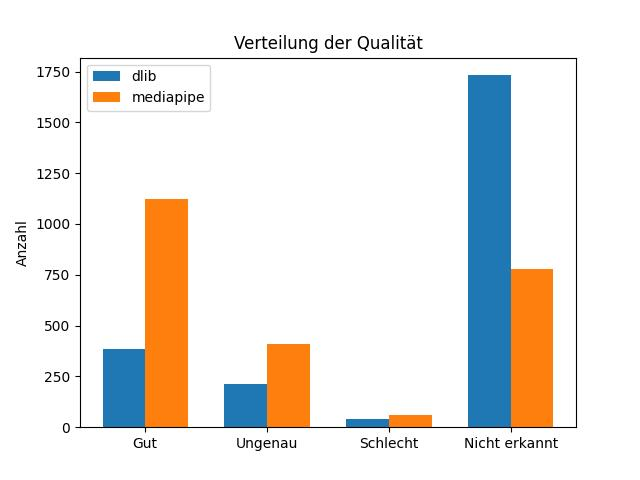
\includegraphics[width=0.7\linewidth]{appendix/11_bar-quality.jpg}
\caption{Aufteilung der Gesichtserkennungsqualität von Video 11.}
\end{figure}

\begin{table}[H]
\centering
\begin{tabular}{l|l|c c |c}
\toprule
\textbf{Gesichtserkennung} & \textbf{Blickrichtung} & \textbf{Seitenlänge} $\hitthresholdsize$ & \textbf{Verschiebung} $\hitthresholdposition$ & \textbf{F1-Score} \\ 
\midrule
\multirow{4}*{dlib}& ETH-XGaze & 0,286 & 0,01 & 0,912  \\ 
& Gaze360 & 0,49 & 0,047 & 0,843 \\ 
& MPIIFaceGaze & 0,112 & -0,002 & 0,721  \\ 
& Kopfrotation & 0,398 & 0,182 & 0,772  \\ 
\hline\multirow{4}*{MediaPipe}& ETH-XGaze & 0,408 & 0,01 & 0,957  \\ 
& Gaze360 & 0,49 & 0,047 & 0,822 \\ 
& MPIIFaceGaze & 0,173 & -0,027 & 0,442  \\ 
& Kopfrotation & 0,5 & 0,218 & 0,865  \\ 
\bottomrule\end{tabular}
\caption{Ergebnis des Hyperparameter-Tunings für die Zone speziell für Video 11.}
\label{tab:appendix:11:local}
\end{table}
\begin{table}[H]
\centering
\begin{tabular}{l|l|c c c c|c c|c}
\toprule
\textbf{Gesichtserkennung} & \textbf{Blickrichtung} & $TP$ & $TN$& $FP$ & $FN$ & \textbf{Precision} & \textbf{Recall} & \textbf{F1-Score} \\ 
\midrule
\multirow{4}*{dlib}& ETH-XGaze & 356 & 1909 & 11 & 85 & 0,97 & 0,807 & 0,881 \\ 
& Gaze360 & 342 & 1892 & 28 & 99 & 0,924 & 0,776 & 0,843 \\ 
& MPIIFaceGaze & 354 & 1726 & 194 & 87 & 0,646 & 0,803 & 0,716 \\ 
& Kopfrotation & 326 & 1785 & 135 & 115 & 0,707 & 0,739 & 0,723 \\ 
\hline\multirow{4}*{MediaPipe}& ETH-XGaze & 404 & 1910 & 15 & 37 & 0,964 & 0,916 & 0,94 \\ 
& Gaze360 & 348 & 1863 & 62 & 93 & 0,849 & 0,789 & 0,818 \\ 
& MPIIFaceGaze & 256 & 1295 & 630 & 185 & 0,289 & 0,58 & 0,386 \\ 
& Kopfrotation & 323 & 1892 & 33 & 118 & 0,907 & 0,732 & 0,811 \\ 
\bottomrule\end{tabular}
\caption{Zusammensetzung des F1-Scores unter Verwendung der in Kapitel \ref{sec:evaluation:results:gaze:threshold} bestimmten globalen Parameter $\hitthresholdsize$ und $\hitthresholdposition$.}
\label{tab:appendix:11:f1}
\end{table}
\begin{figure}[H]
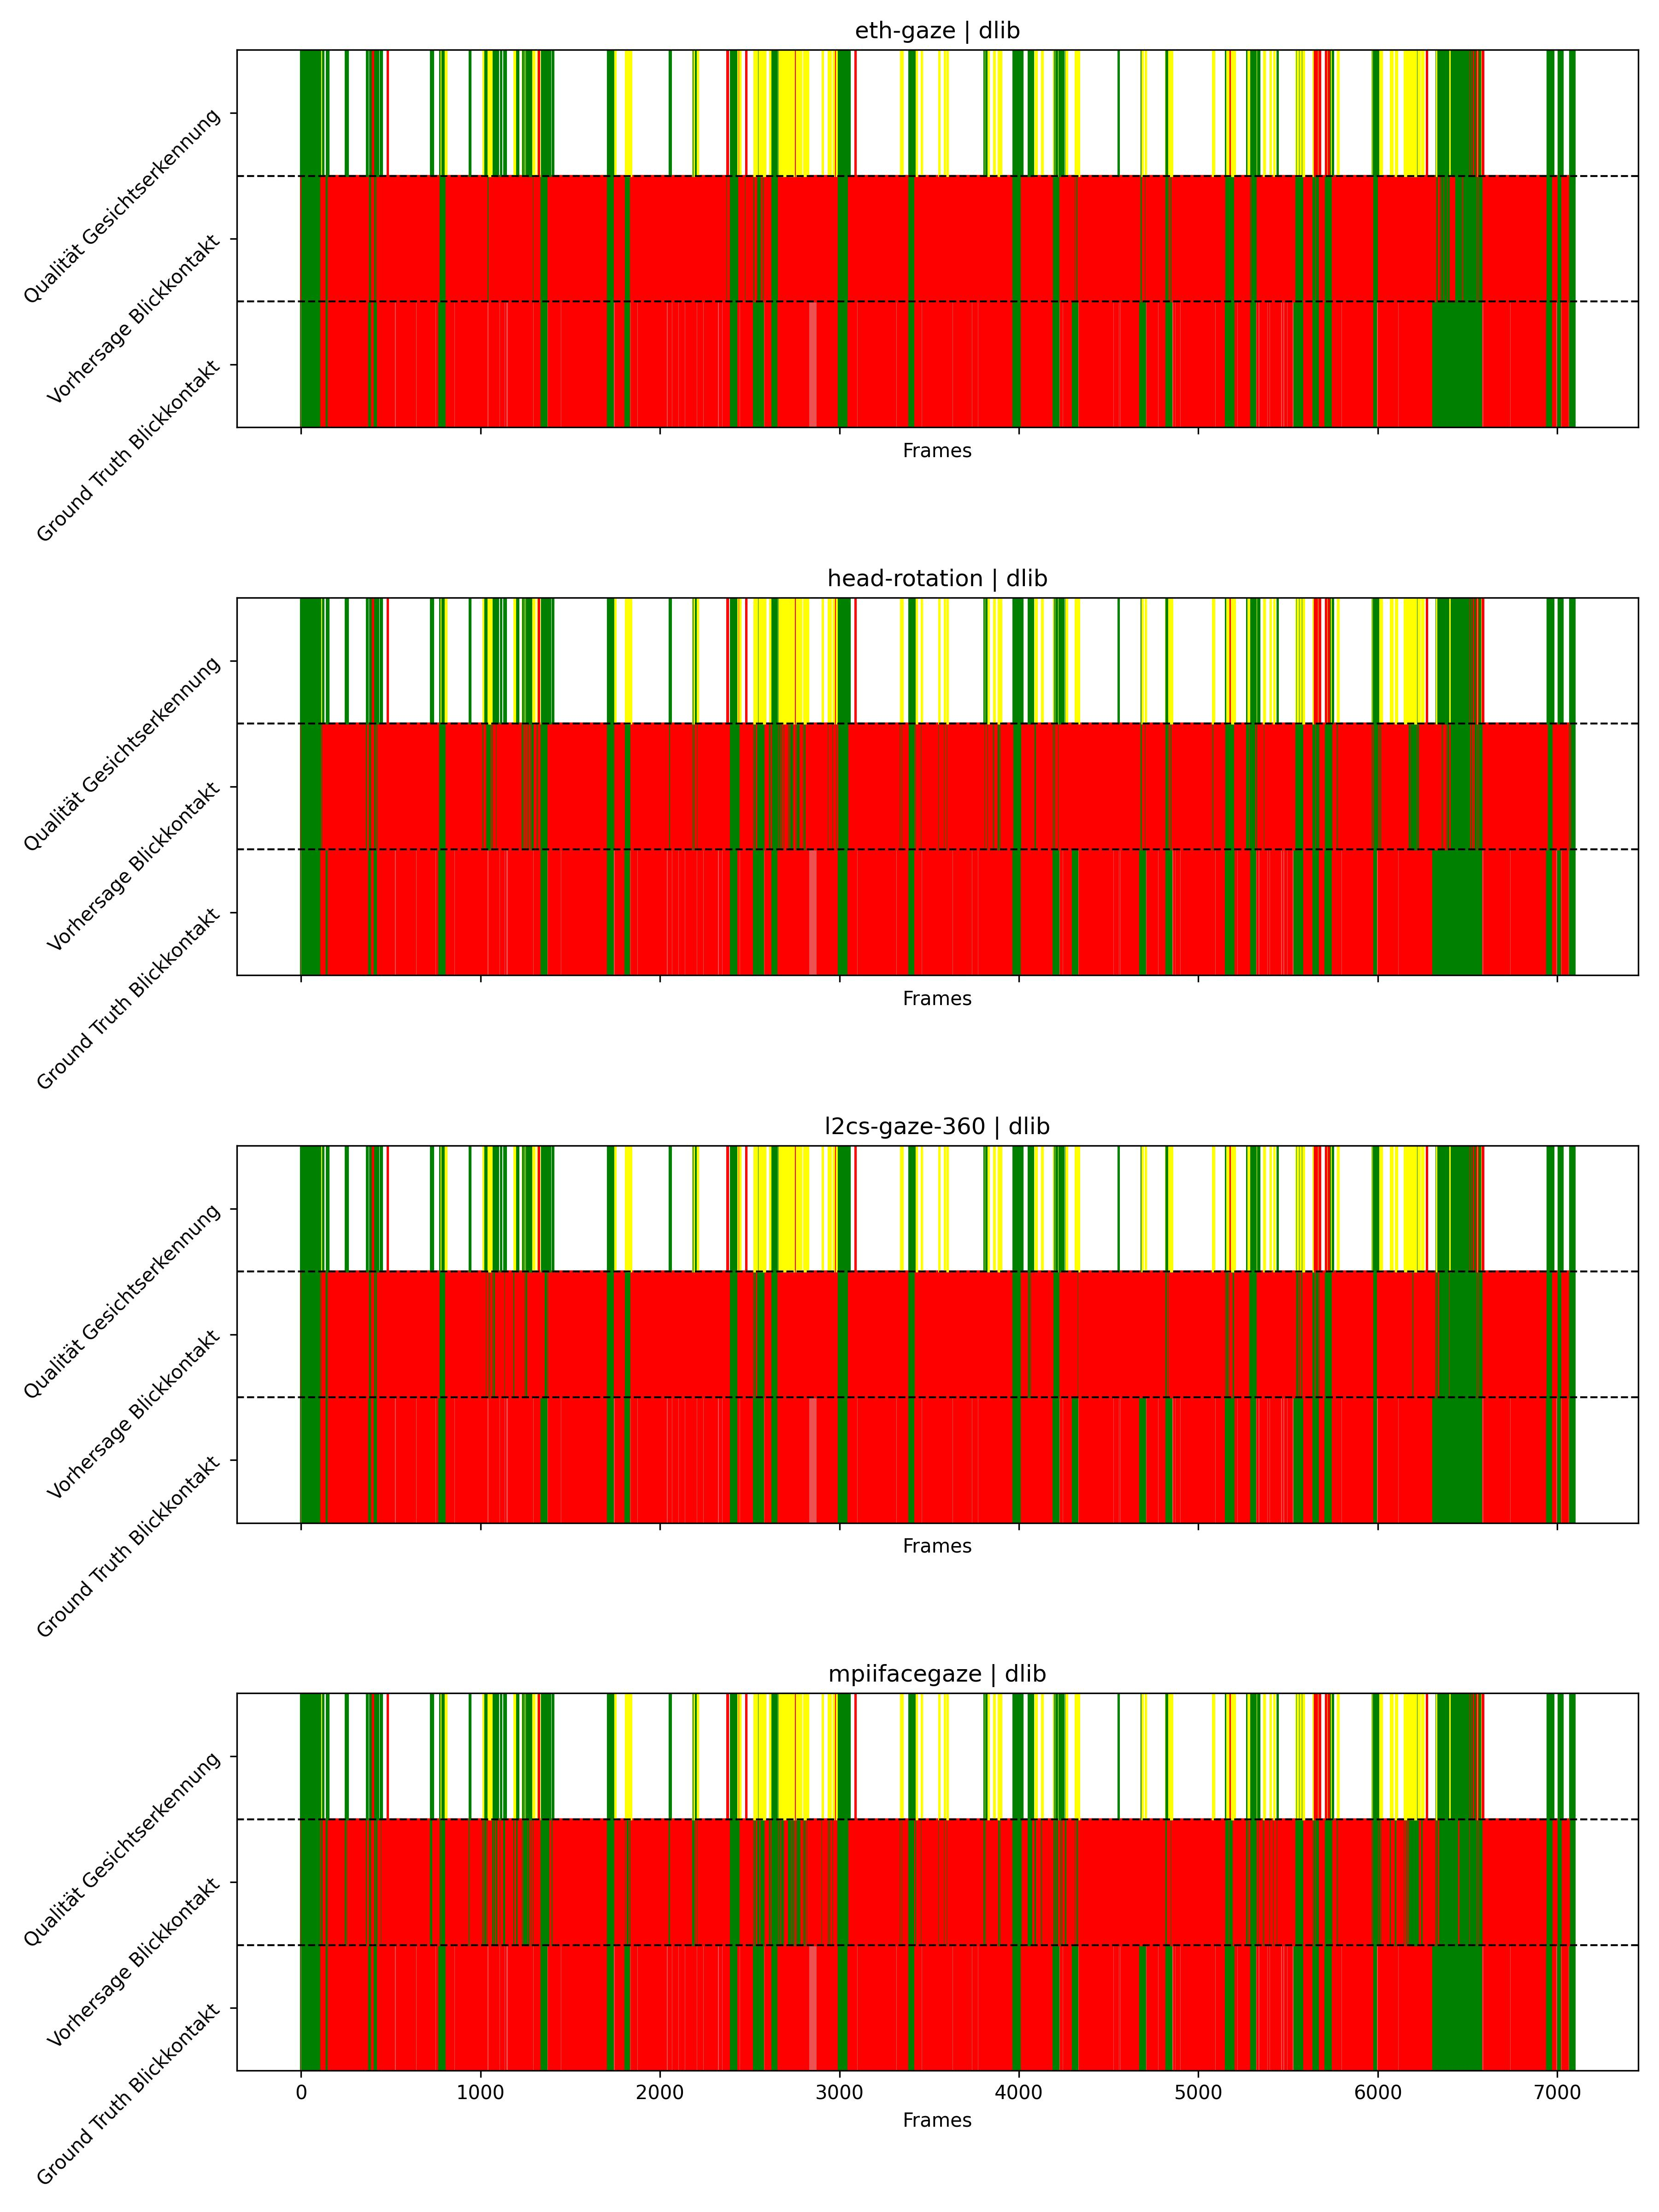
\includegraphics[width=1\linewidth]{appendix/11-dlib-overview-gaze.jpg}
\caption{Überblick über die Ground Truth des Blickkontakts, die Vorhersage des Blickkontakts und die Qualität der Gesichtserkennung mit \dlib. Die Bedeutung der Farben ist in Abbildung \ref{fig:evaluation:gaze:mpiifacegaze} erklärt.  }
\end{figure}

\begin{figure}[H]
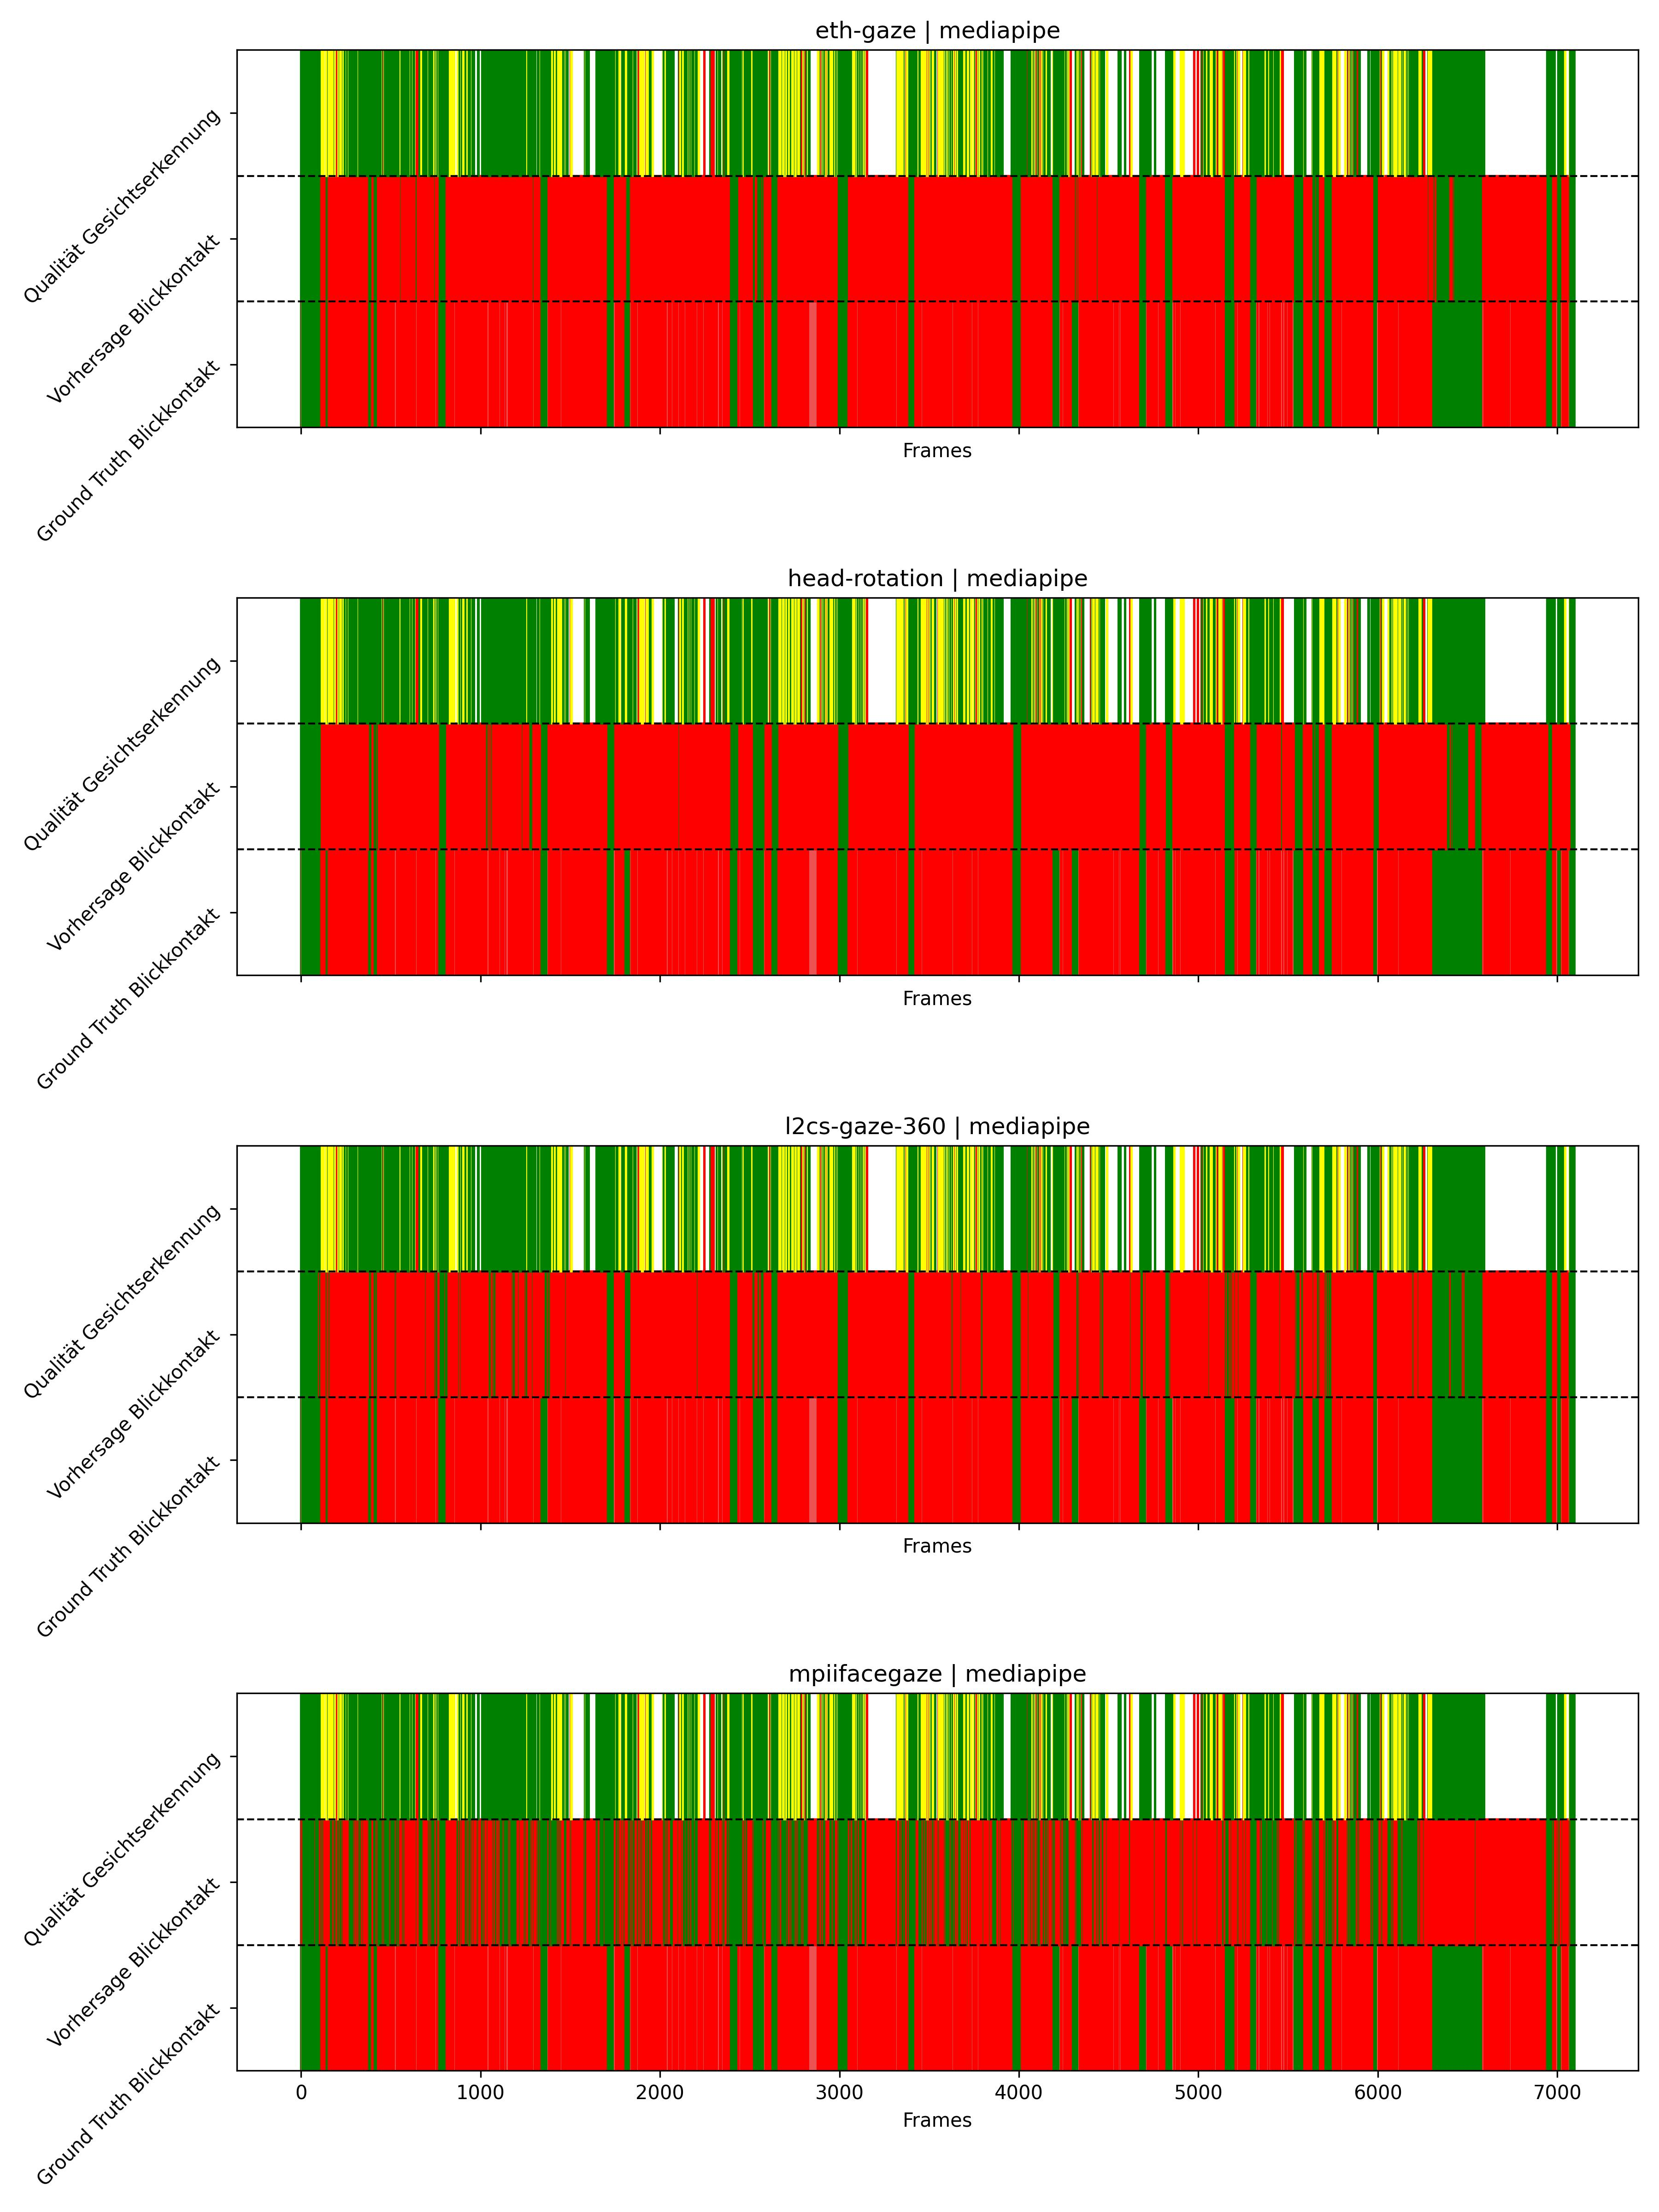
\includegraphics[width=1\linewidth]{appendix/11-mediapipe-overview-gaze.jpg}
\caption{Überblick über die Ground Truth des Blickkontakts, die Vorhersage des Blickkontakts und die Qualität der Gesichtserkennung mit \mediapipe. Die Bedeutung der Farben ist in Abbildung \ref{fig:evaluation:gaze:mpiifacegaze} erklärt.}
\end{figure}

\section{Video 12}
\begin{figure}[H]
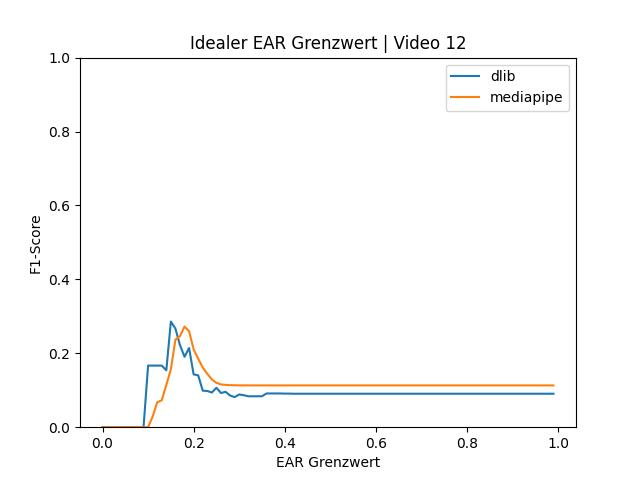
\includegraphics[width=0.7\linewidth]{appendix/12_f1-score-blink.jpg}
\caption{Ergebnisse der Bestimmung des idealen EAR-Grenzwerts für Video 12.}
\end{figure}

\begin{figure}[H]
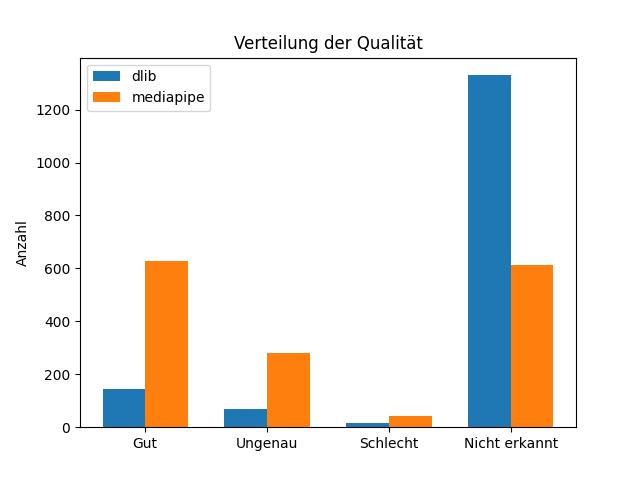
\includegraphics[width=0.7\linewidth]{appendix/12_bar-quality.jpg}
\caption{Aufteilung der Gesichtserkennungsqualität von Video 12.}
\end{figure}

\begin{table}[H]
\centering
\begin{tabular}{l|l|c c |c}
\toprule
\textbf{Gesichtserkennung} & \textbf{Blickrichtung} & \textbf{Seitenlänge} $\hitthresholdsize$ & \textbf{Verschiebung} $\hitthresholdposition$ & \textbf{F1-Score} \\ 
\midrule
\multirow{4}*{dlib}& ETH-XGaze & 0,224 & -0,002 & 0,966  \\ 
& Gaze360 & 0,306 & 0,035 & 0,917 \\ 
& MPIIFaceGaze & 0,051 & -0,027 & 0,774  \\ 
& Kopfrotation & 0,255 & 0,194 & 0,787  \\ 
\hline\multirow{4}*{MediaPipe}& ETH-XGaze & 0,255 & -0,002 & 0,981  \\ 
& Gaze360 & 0,367 & 0,035 & 0,815 \\ 
& MPIIFaceGaze & 0,02 & -0,039 & 0,428  \\ 
& Kopfrotation & 0,194 & 0,194 & 0,899  \\ 
\bottomrule\end{tabular}
\caption{Ergebnis des Hyperparameter-Tunings für die Zone speziell für Video 12.}
\label{tab:appendix:12:local}
\end{table}
\begin{table}[H]
\centering
\begin{tabular}{l|l|c c c c|c c|c}
\toprule
\textbf{Gesichtserkennung} & \textbf{Blickrichtung} & $TP$ & $TN$& $FP$ & $FN$ & \textbf{Precision} & \textbf{Recall} & \textbf{F1-Score} \\ 
\midrule
\multirow{4}*{dlib}& ETH-XGaze & 125 & 1424 & 6 & 7 & 0,954 & 0,947 & 0,951 \\ 
& Gaze360 & 120 & 1417 & 13 & 12 & 0,902 & 0,909 & 0,906 \\ 
& MPIIFaceGaze & 123 & 1362 & 68 & 9 & 0,644 & 0,932 & 0,762 \\ 
& Kopfrotation & 126 & 1360 & 70 & 6 & 0,643 & 0,955 & 0,768 \\ 
\hline\multirow{4}*{MediaPipe}& ETH-XGaze & 132 & 1424 & 6 & 0 & 0,957 & 1,0 & 0,978 \\ 
& Gaze360 & 113 & 1387 & 43 & 19 & 0,724 & 0,856 & 0,785 \\ 
& MPIIFaceGaze & 125 & 888 & 542 & 7 & 0,187 & 0,947 & 0,313 \\ 
& Kopfrotation & 123 & 1408 & 22 & 9 & 0,848 & 0,932 & 0,888 \\ 
\bottomrule\end{tabular}
\caption{Zusammensetzung des F1-Scores unter Verwendung der in Kapitel \ref{sec:evaluation:results:gaze:threshold} bestimmten globalen Parameter $\hitthresholdsize$ und $\hitthresholdposition$.}
\label{tab:appendix:12:f1}
\end{table}
\begin{figure}[H]
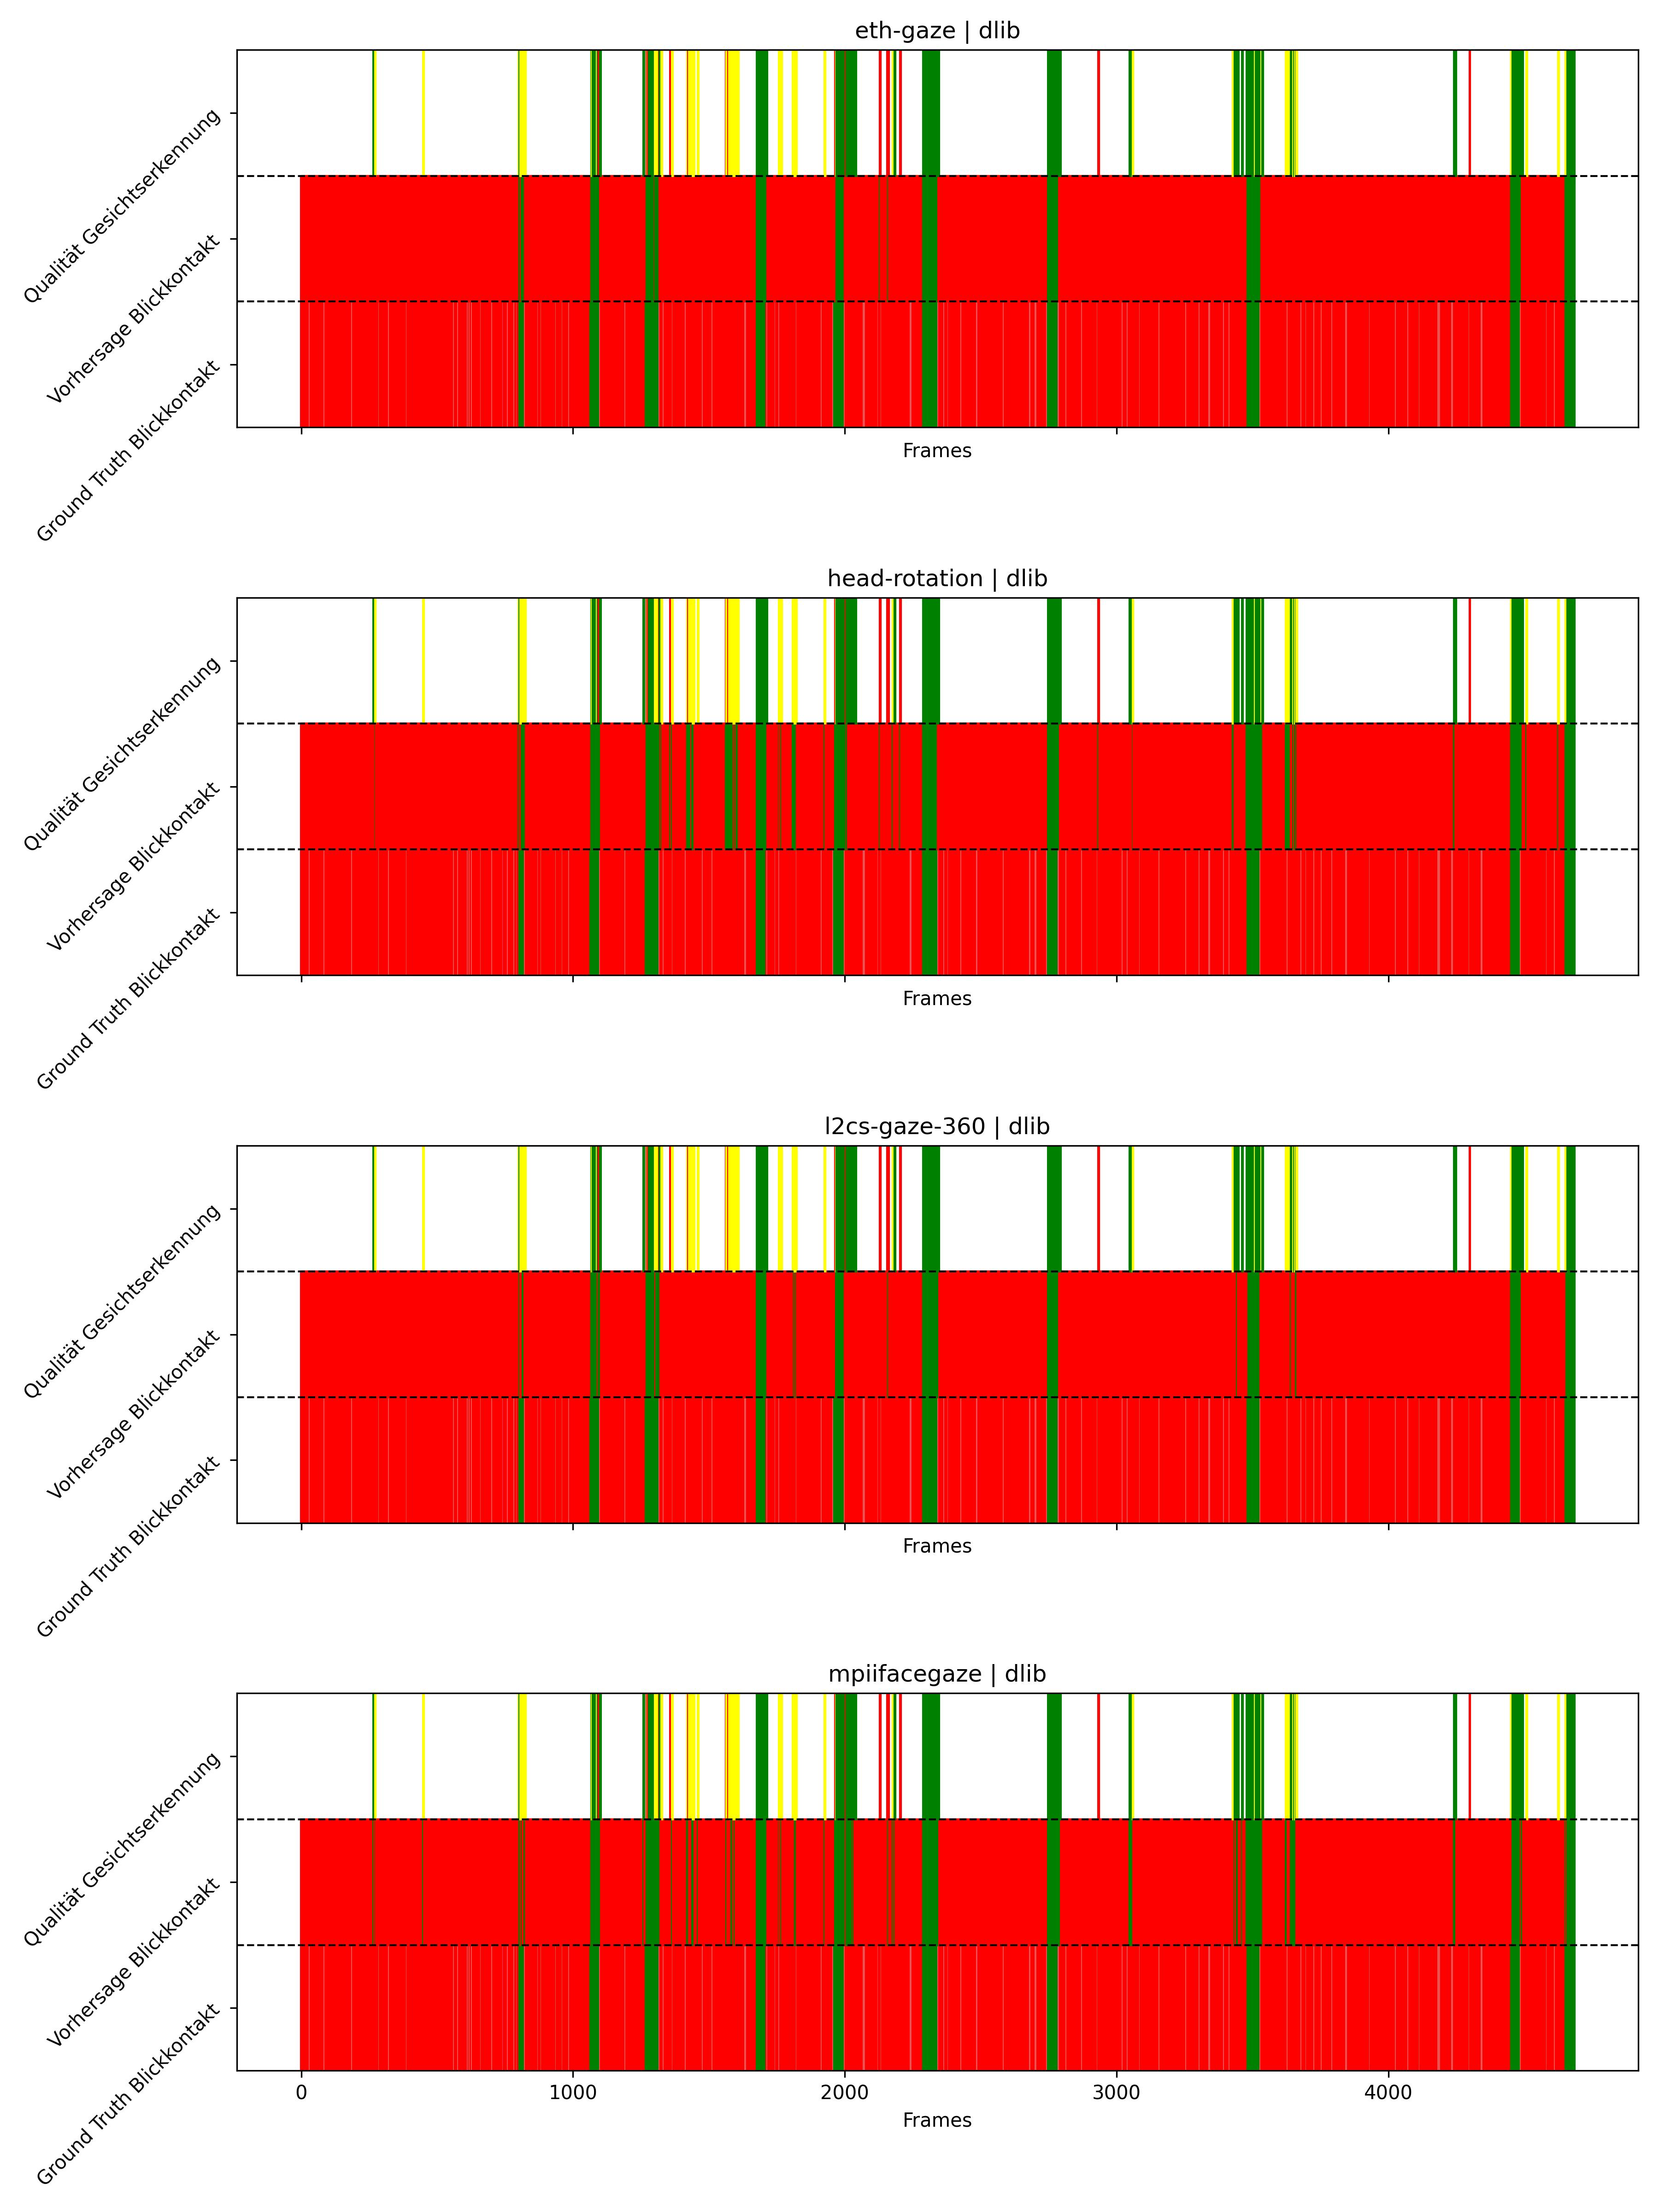
\includegraphics[width=1\linewidth]{appendix/12-dlib-overview-gaze.jpg}
\caption{Überblick über die Ground Truth des Blickkontakts, die Vorhersage des Blickkontakts und die Qualität der Gesichtserkennung mit \dlib. Die Bedeutung der Farben ist in Abbildung \ref{fig:evaluation:gaze:mpiifacegaze} erklärt.  }
\end{figure}

\begin{figure}[H]
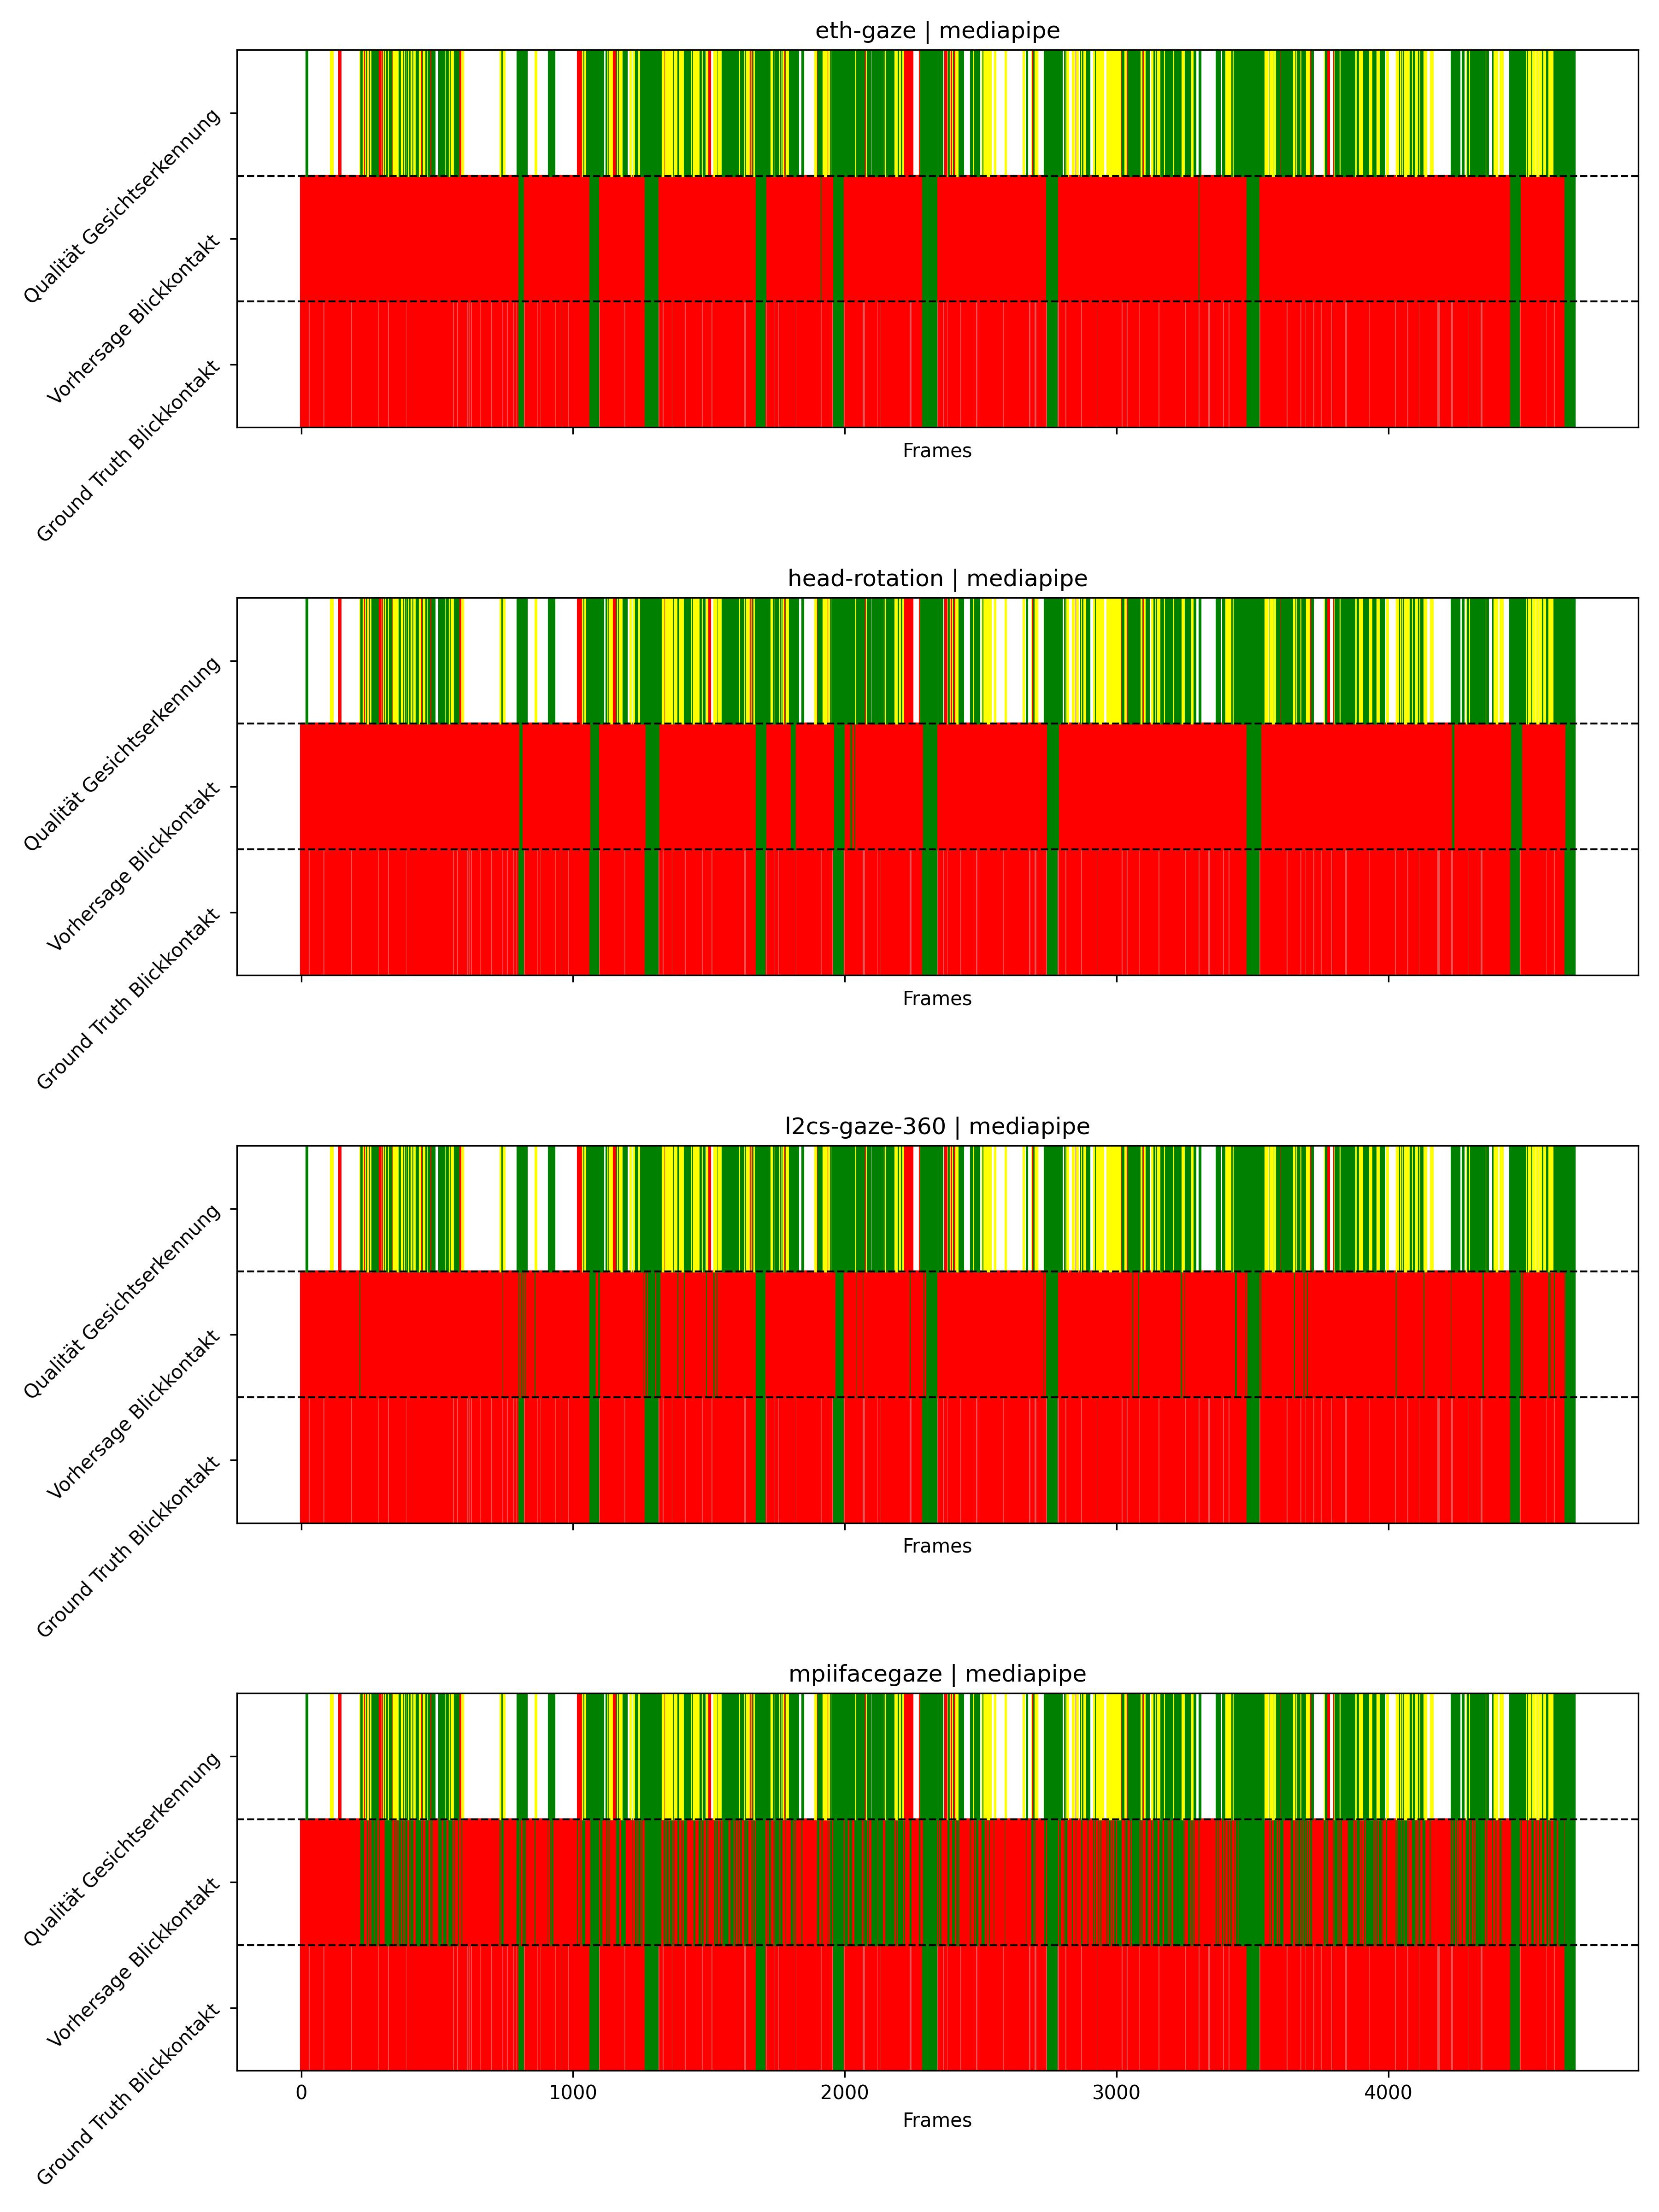
\includegraphics[width=1\linewidth]{appendix/12-mediapipe-overview-gaze.jpg}
\caption{Überblick über die Ground Truth des Blickkontakts, die Vorhersage des Blickkontakts und die Qualität der Gesichtserkennung mit \mediapipe. Die Bedeutung der Farben ist in Abbildung \ref{fig:evaluation:gaze:mpiifacegaze} erklärt.}
\end{figure}

\section{Video 13}
\begin{figure}[H]
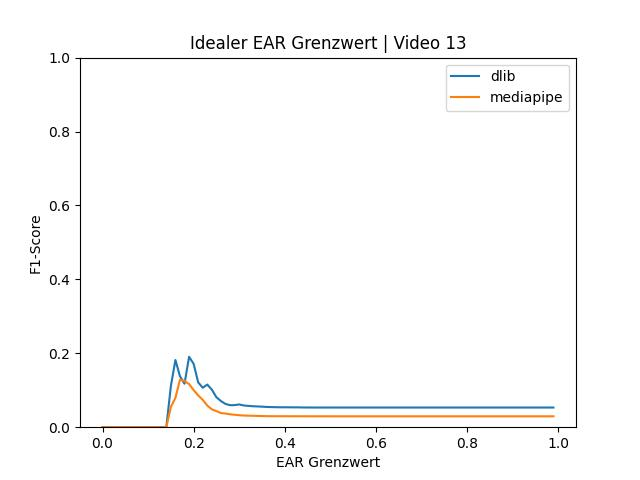
\includegraphics[width=0.7\linewidth]{appendix/13_f1-score-blink.jpg}
\caption{Ergebnisse der Bestimmung des idealen EAR-Grenzwerts für Video 13.}
\end{figure}

\begin{figure}[H]
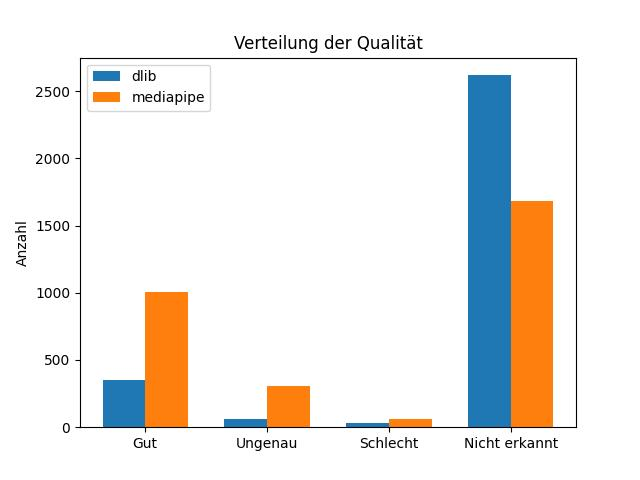
\includegraphics[width=0.7\linewidth]{appendix/13_bar-quality.jpg}
\caption{Aufteilung der Gesichtserkennungsqualität von Video 13.}
\end{figure}

\begin{table}[H]
\centering
\begin{tabular}{l|l|c c |c}
\toprule
\textbf{Gesichtserkennung} & \textbf{Blickrichtung} & \textbf{Seitenlänge} $\hitthresholdsize$ & \textbf{Verschiebung} $\hitthresholdposition$ & \textbf{F1-Score} \\ 
\midrule
\multirow{4}*{dlib}& ETH-XGaze & 0,194 & -0,002 & 0,929  \\ 
& Gaze360 & 0,224 & 0,071 & 0,885 \\ 
& MPIIFaceGaze & 0,082 & -0,027 & 0,827  \\ 
& Kopfrotation & 0,316 & 0,206 & 0,84  \\ 
\hline\multirow{4}*{MediaPipe}& ETH-XGaze & 0,184 & -0,002 & 0,977  \\ 
& Gaze360 & 0,378 & 0,047 & 0,875 \\ 
& MPIIFaceGaze & 0,041 & -0,027 & 0,478  \\ 
& Kopfrotation & 0,357 & 0,206 & 0,932  \\ 
\bottomrule\end{tabular}
\caption{Ergebnis des Hyperparameter-Tunings für die Zone speziell für Video 13.}
\label{tab:appendix:13:local}
\end{table}
\begin{table}[H]
\centering
\begin{tabular}{l|l|c c c c|c c|c}
\toprule
\textbf{Gesichtserkennung} & \textbf{Blickrichtung} & $TP$ & $TN$& $FP$ & $FN$ & \textbf{Precision} & \textbf{Recall} & \textbf{F1-Score} \\ 
\midrule
\multirow{4}*{dlib}& ETH-XGaze & 321 & 2680 & 9 & 45 & 0,973 & 0,877 & 0,922 \\ 
& Gaze360 & 314 & 2658 & 31 & 52 & 0,91 & 0,858 & 0,883 \\ 
& MPIIFaceGaze & 317 & 2604 & 85 & 49 & 0,789 & 0,866 & 0,826 \\ 
& Kopfrotation & 307 & 2621 & 68 & 59 & 0,819 & 0,839 & 0,829 \\ 
\hline\multirow{4}*{MediaPipe}& ETH-XGaze & 363 & 2660 & 32 & 3 & 0,919 & 0,992 & 0,954 \\ 
& Gaze360 & 348 & 2610 & 82 & 18 & 0,809 & 0,951 & 0,874 \\ 
& MPIIFaceGaze & 290 & 2091 & 601 & 76 & 0,325 & 0,792 & 0,461 \\ 
& Kopfrotation & 316 & 2659 & 33 & 50 & 0,905 & 0,863 & 0,884 \\ 
\bottomrule\end{tabular}
\caption{Zusammensetzung des F1-Scores unter Verwendung der in Kapitel \ref{sec:evaluation:results:gaze:threshold} bestimmten globalen Parameter $\hitthresholdsize$ und $\hitthresholdposition$.}
\label{tab:appendix:13:f1}
\end{table}
\begin{figure}[H]
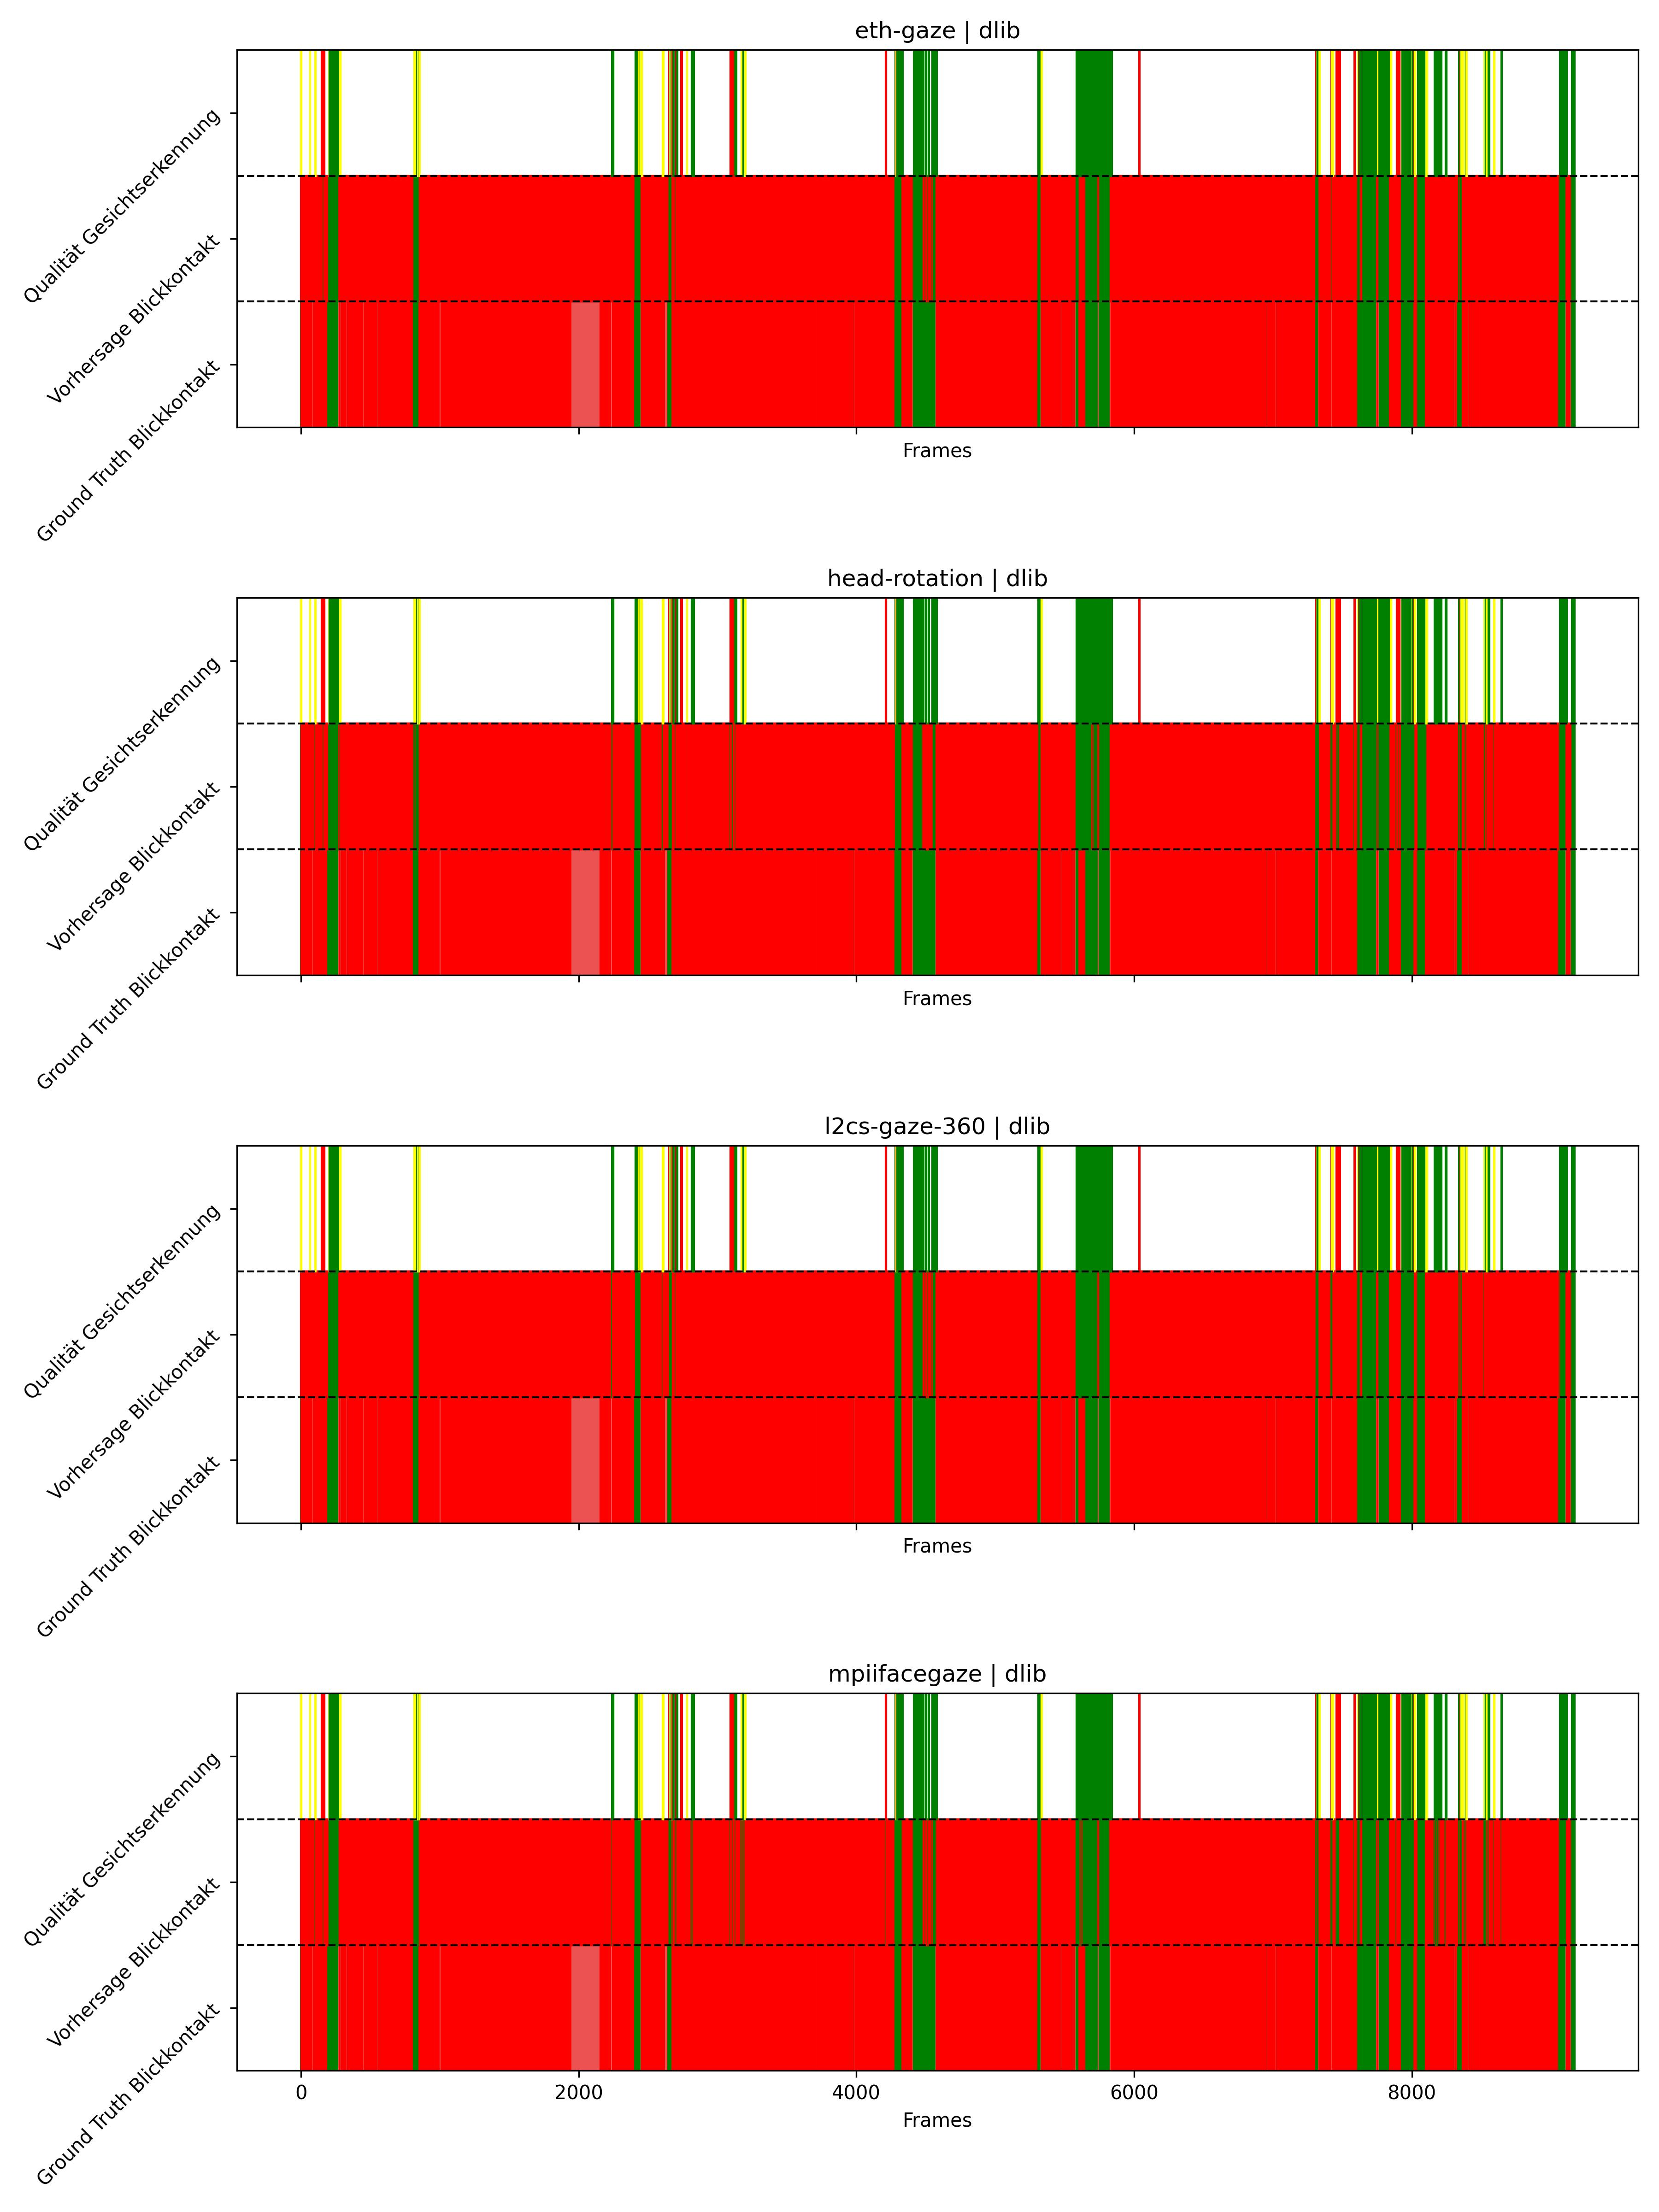
\includegraphics[width=1\linewidth]{appendix/13-dlib-overview-gaze.jpg}
\caption{Überblick über die Ground Truth des Blickkontakts, die Vorhersage des Blickkontakts und die Qualität der Gesichtserkennung mit \dlib. Die Bedeutung der Farben ist in Abbildung \ref{fig:evaluation:gaze:mpiifacegaze} erklärt.  }
\end{figure}

\begin{figure}[H]
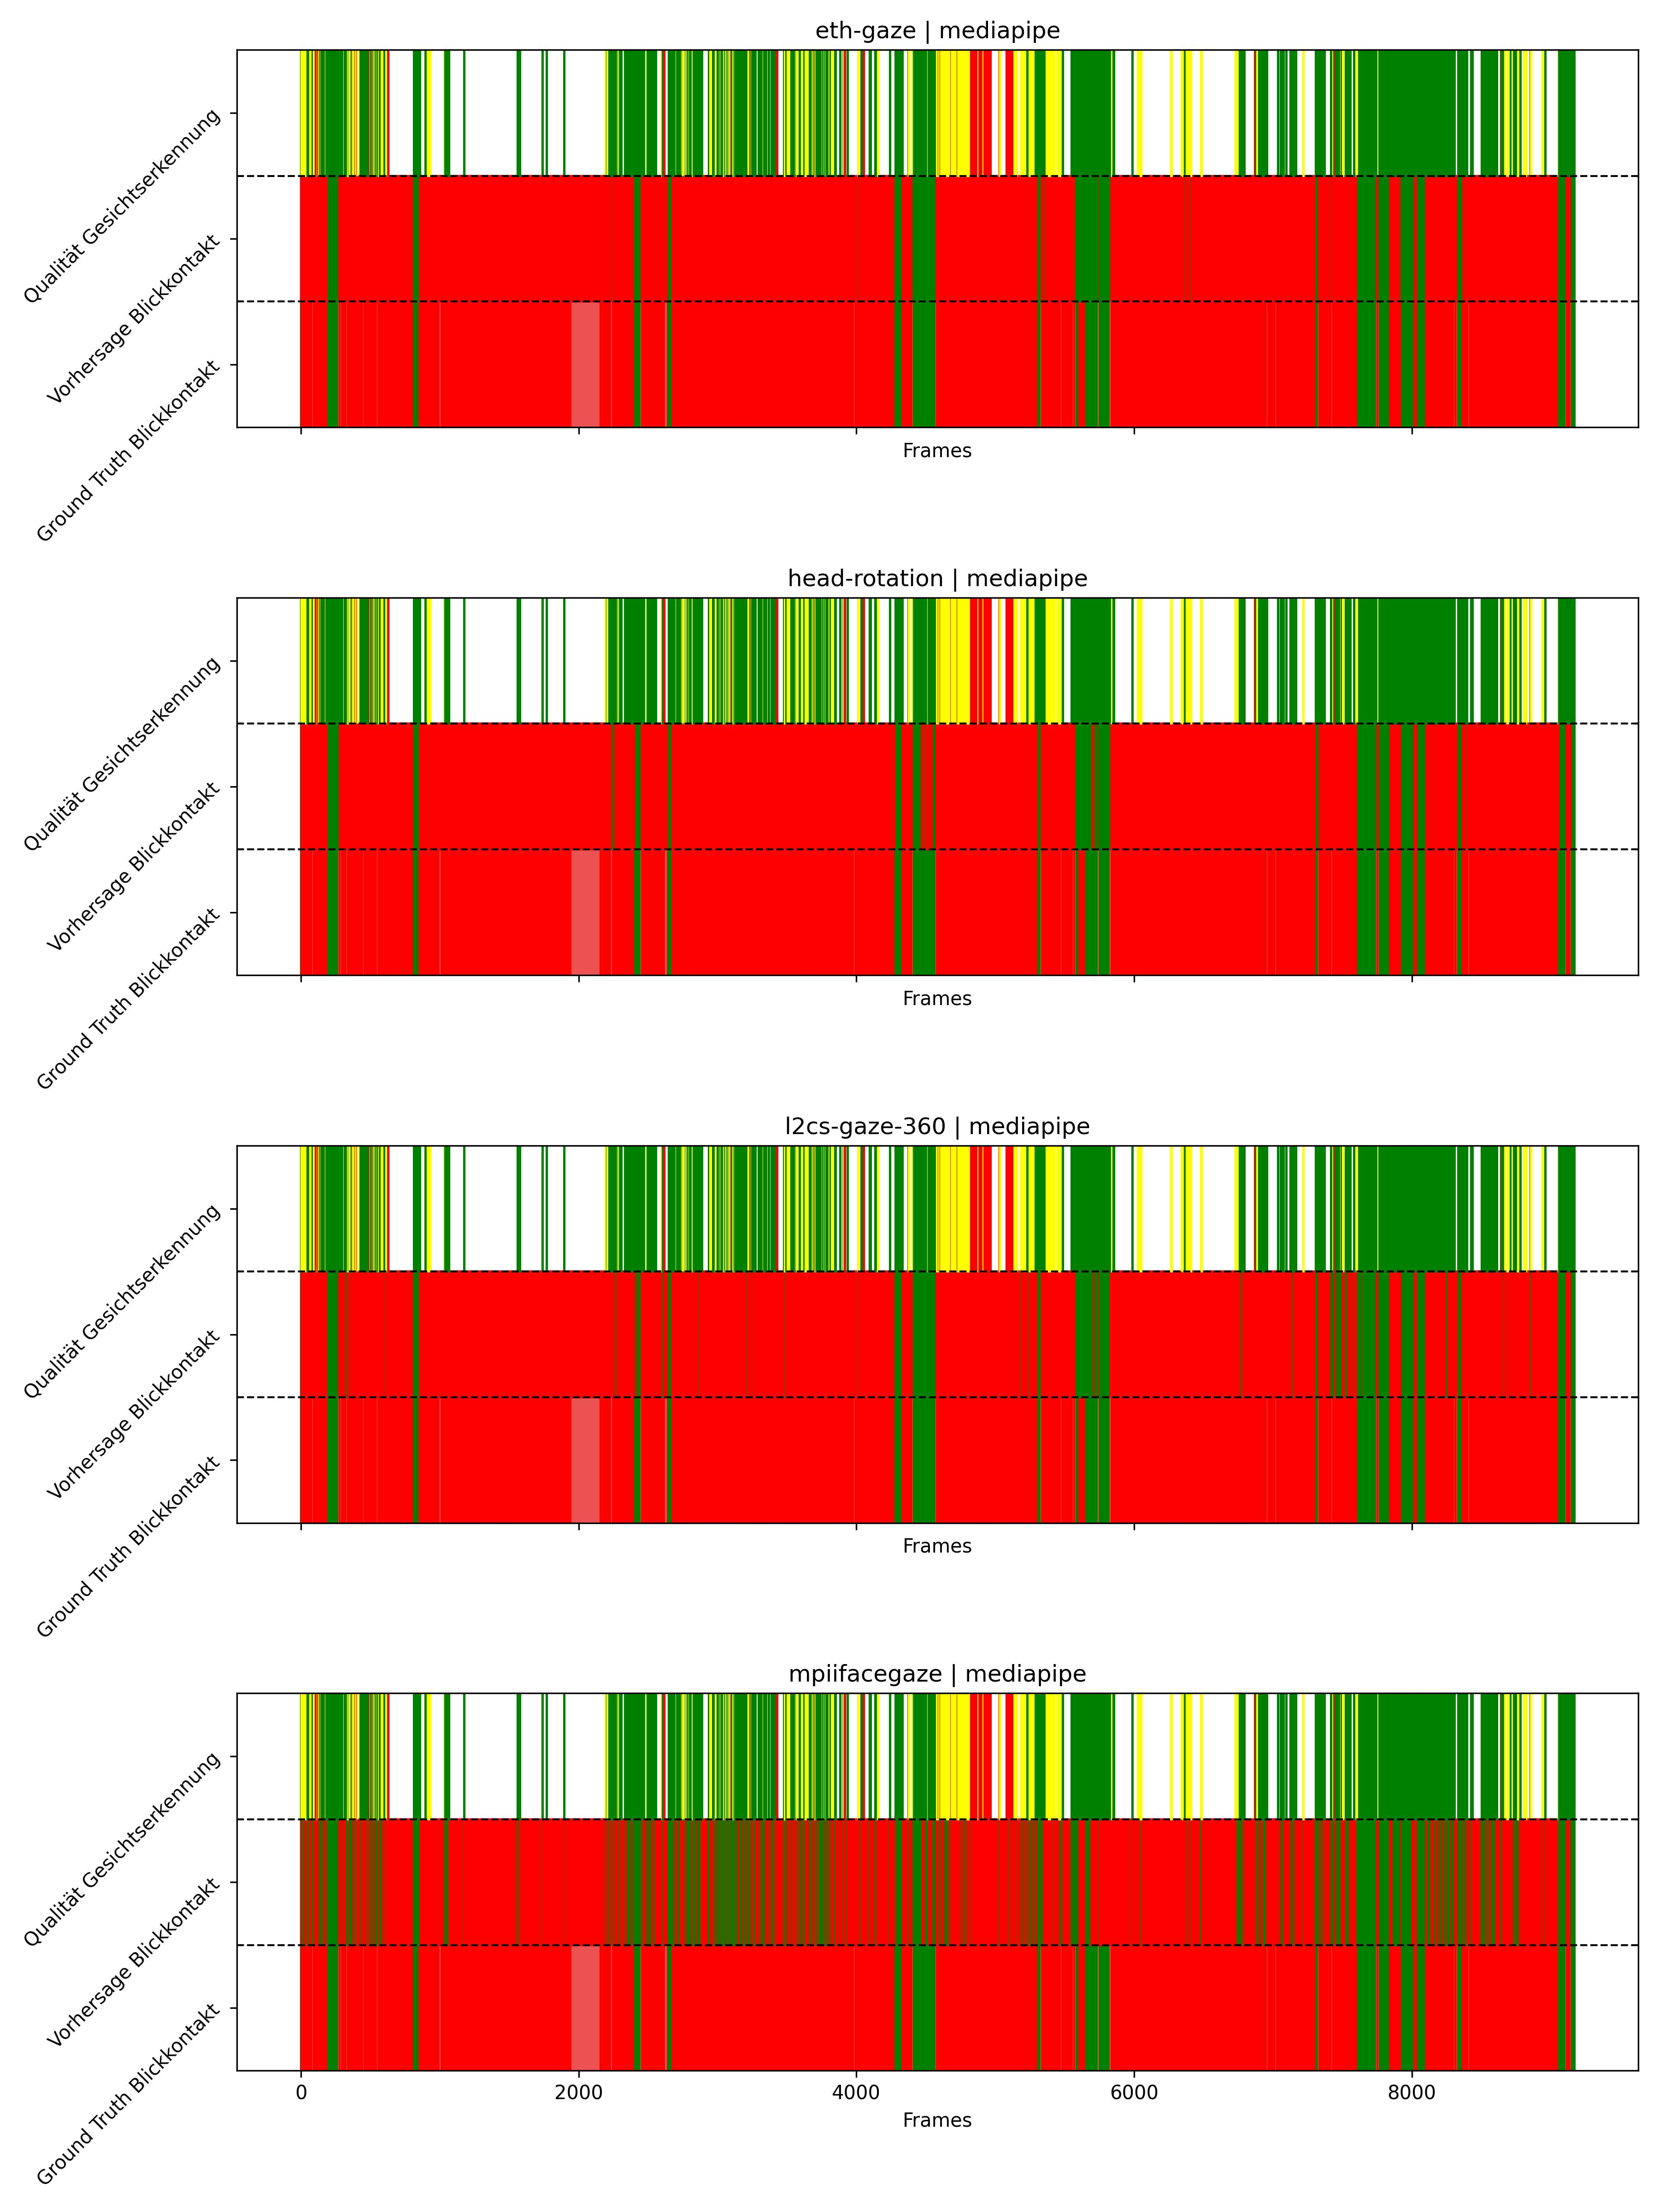
\includegraphics[width=1\linewidth]{appendix/13-mediapipe-overview-gaze.jpg}
\caption{Überblick über die Ground Truth des Blickkontakts, die Vorhersage des Blickkontakts und die Qualität der Gesichtserkennung mit \mediapipe. Die Bedeutung der Farben ist in Abbildung \ref{fig:evaluation:gaze:mpiifacegaze} erklärt.}
\end{figure}

\section{Video 14}
\begin{figure}[H]
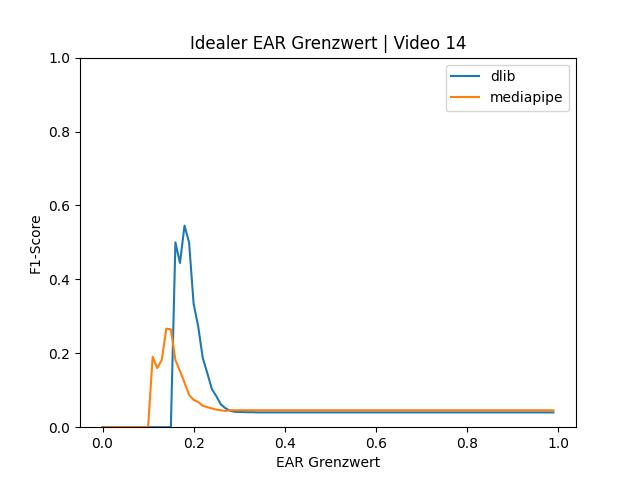
\includegraphics[width=0.7\linewidth]{appendix/14_f1-score-blink.jpg}
\caption{Ergebnisse der Bestimmung des idealen EAR-Grenzwerts für Video 14.}
\end{figure}

\begin{figure}[H]
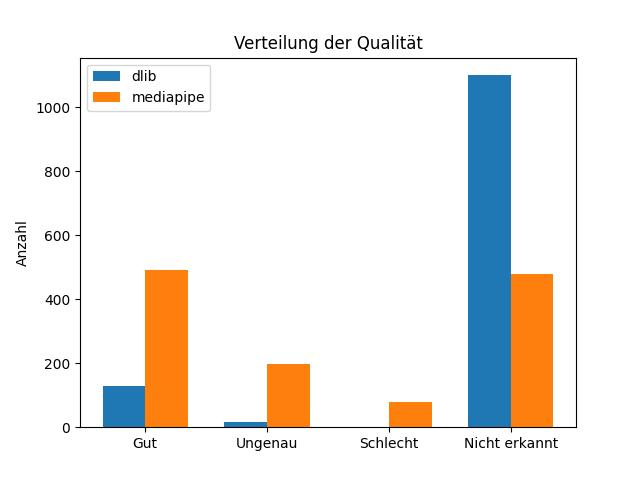
\includegraphics[width=0.7\linewidth]{appendix/14_bar-quality.jpg}
\caption{Aufteilung der Gesichtserkennungsqualität von Video 14.}
\end{figure}

\begin{table}[H]
\centering
\begin{tabular}{l|l|c c |c}
\toprule
\textbf{Gesichtserkennung} & \textbf{Blickrichtung} & \textbf{Seitenlänge} $\hitthresholdsize$ & \textbf{Verschiebung} $\hitthresholdposition$ & \textbf{F1-Score} \\ 
\midrule
\multirow{4}*{dlib}& ETH-XGaze & 0,204 & 0,01 & 0,756  \\ 
& Gaze360 & 0,347 & 0,047 & 0,75 \\ 
& MPIIFaceGaze & 0,061 & -0,014 & 0,709  \\ 
& Kopfrotation & 0,306 & 0,206 & 0,723  \\ 
\hline\multirow{4}*{MediaPipe}& ETH-XGaze & 0,163 & 0,047 & 0,925  \\ 
& Gaze360 & 0,48 & 0,035 & 0,737 \\ 
& MPIIFaceGaze & 0,092 & 0,035 & 0,458  \\ 
& Kopfrotation & 0,224 & 0,218 & 0,881  \\ 
\bottomrule\end{tabular}
\caption{Ergebnis des Hyperparameter-Tunings für die Zone speziell für Video 14.}
\label{tab:appendix:14:local}
\end{table}
\begin{table}[H]
\centering
\begin{tabular}{l|l|c c c c|c c|c}
\toprule
\textbf{Gesichtserkennung} & \textbf{Blickrichtung} & $TP$ & $TN$& $FP$ & $FN$ & \textbf{Precision} & \textbf{Recall} & \textbf{F1-Score} \\ 
\midrule
\multirow{4}*{dlib}& ETH-XGaze & 121 & 1046 & 1 & 78 & 0,992 & 0,608 & 0,754 \\ 
& Gaze360 & 120 & 1046 & 1 & 79 & 0,992 & 0,603 & 0,75 \\ 
& MPIIFaceGaze & 118 & 1026 & 21 & 81 & 0,849 & 0,593 & 0,698 \\ 
& Kopfrotation & 119 & 1034 & 13 & 80 & 0,902 & 0,598 & 0,719 \\ 
\hline\multirow{4}*{MediaPipe}& ETH-XGaze & 172 & 1048 & 1 & 27 & 0,994 & 0,864 & 0,925 \\ 
& Gaze360 & 122 & 1031 & 18 & 77 & 0,871 & 0,613 & 0,72 \\ 
& MPIIFaceGaze & 152 & 632 & 417 & 47 & 0,267 & 0,764 & 0,396 \\ 
& Kopfrotation & 164 & 1037 & 12 & 35 & 0,932 & 0,824 & 0,875 \\ 
\bottomrule\end{tabular}
\caption{Zusammensetzung des F1-Scores unter Verwendung der in Kapitel \ref{sec:evaluation:results:gaze:threshold} bestimmten globalen Parameter $\hitthresholdsize$ und $\hitthresholdposition$.}
\label{tab:appendix:14:f1}
\end{table}
\begin{figure}[H]
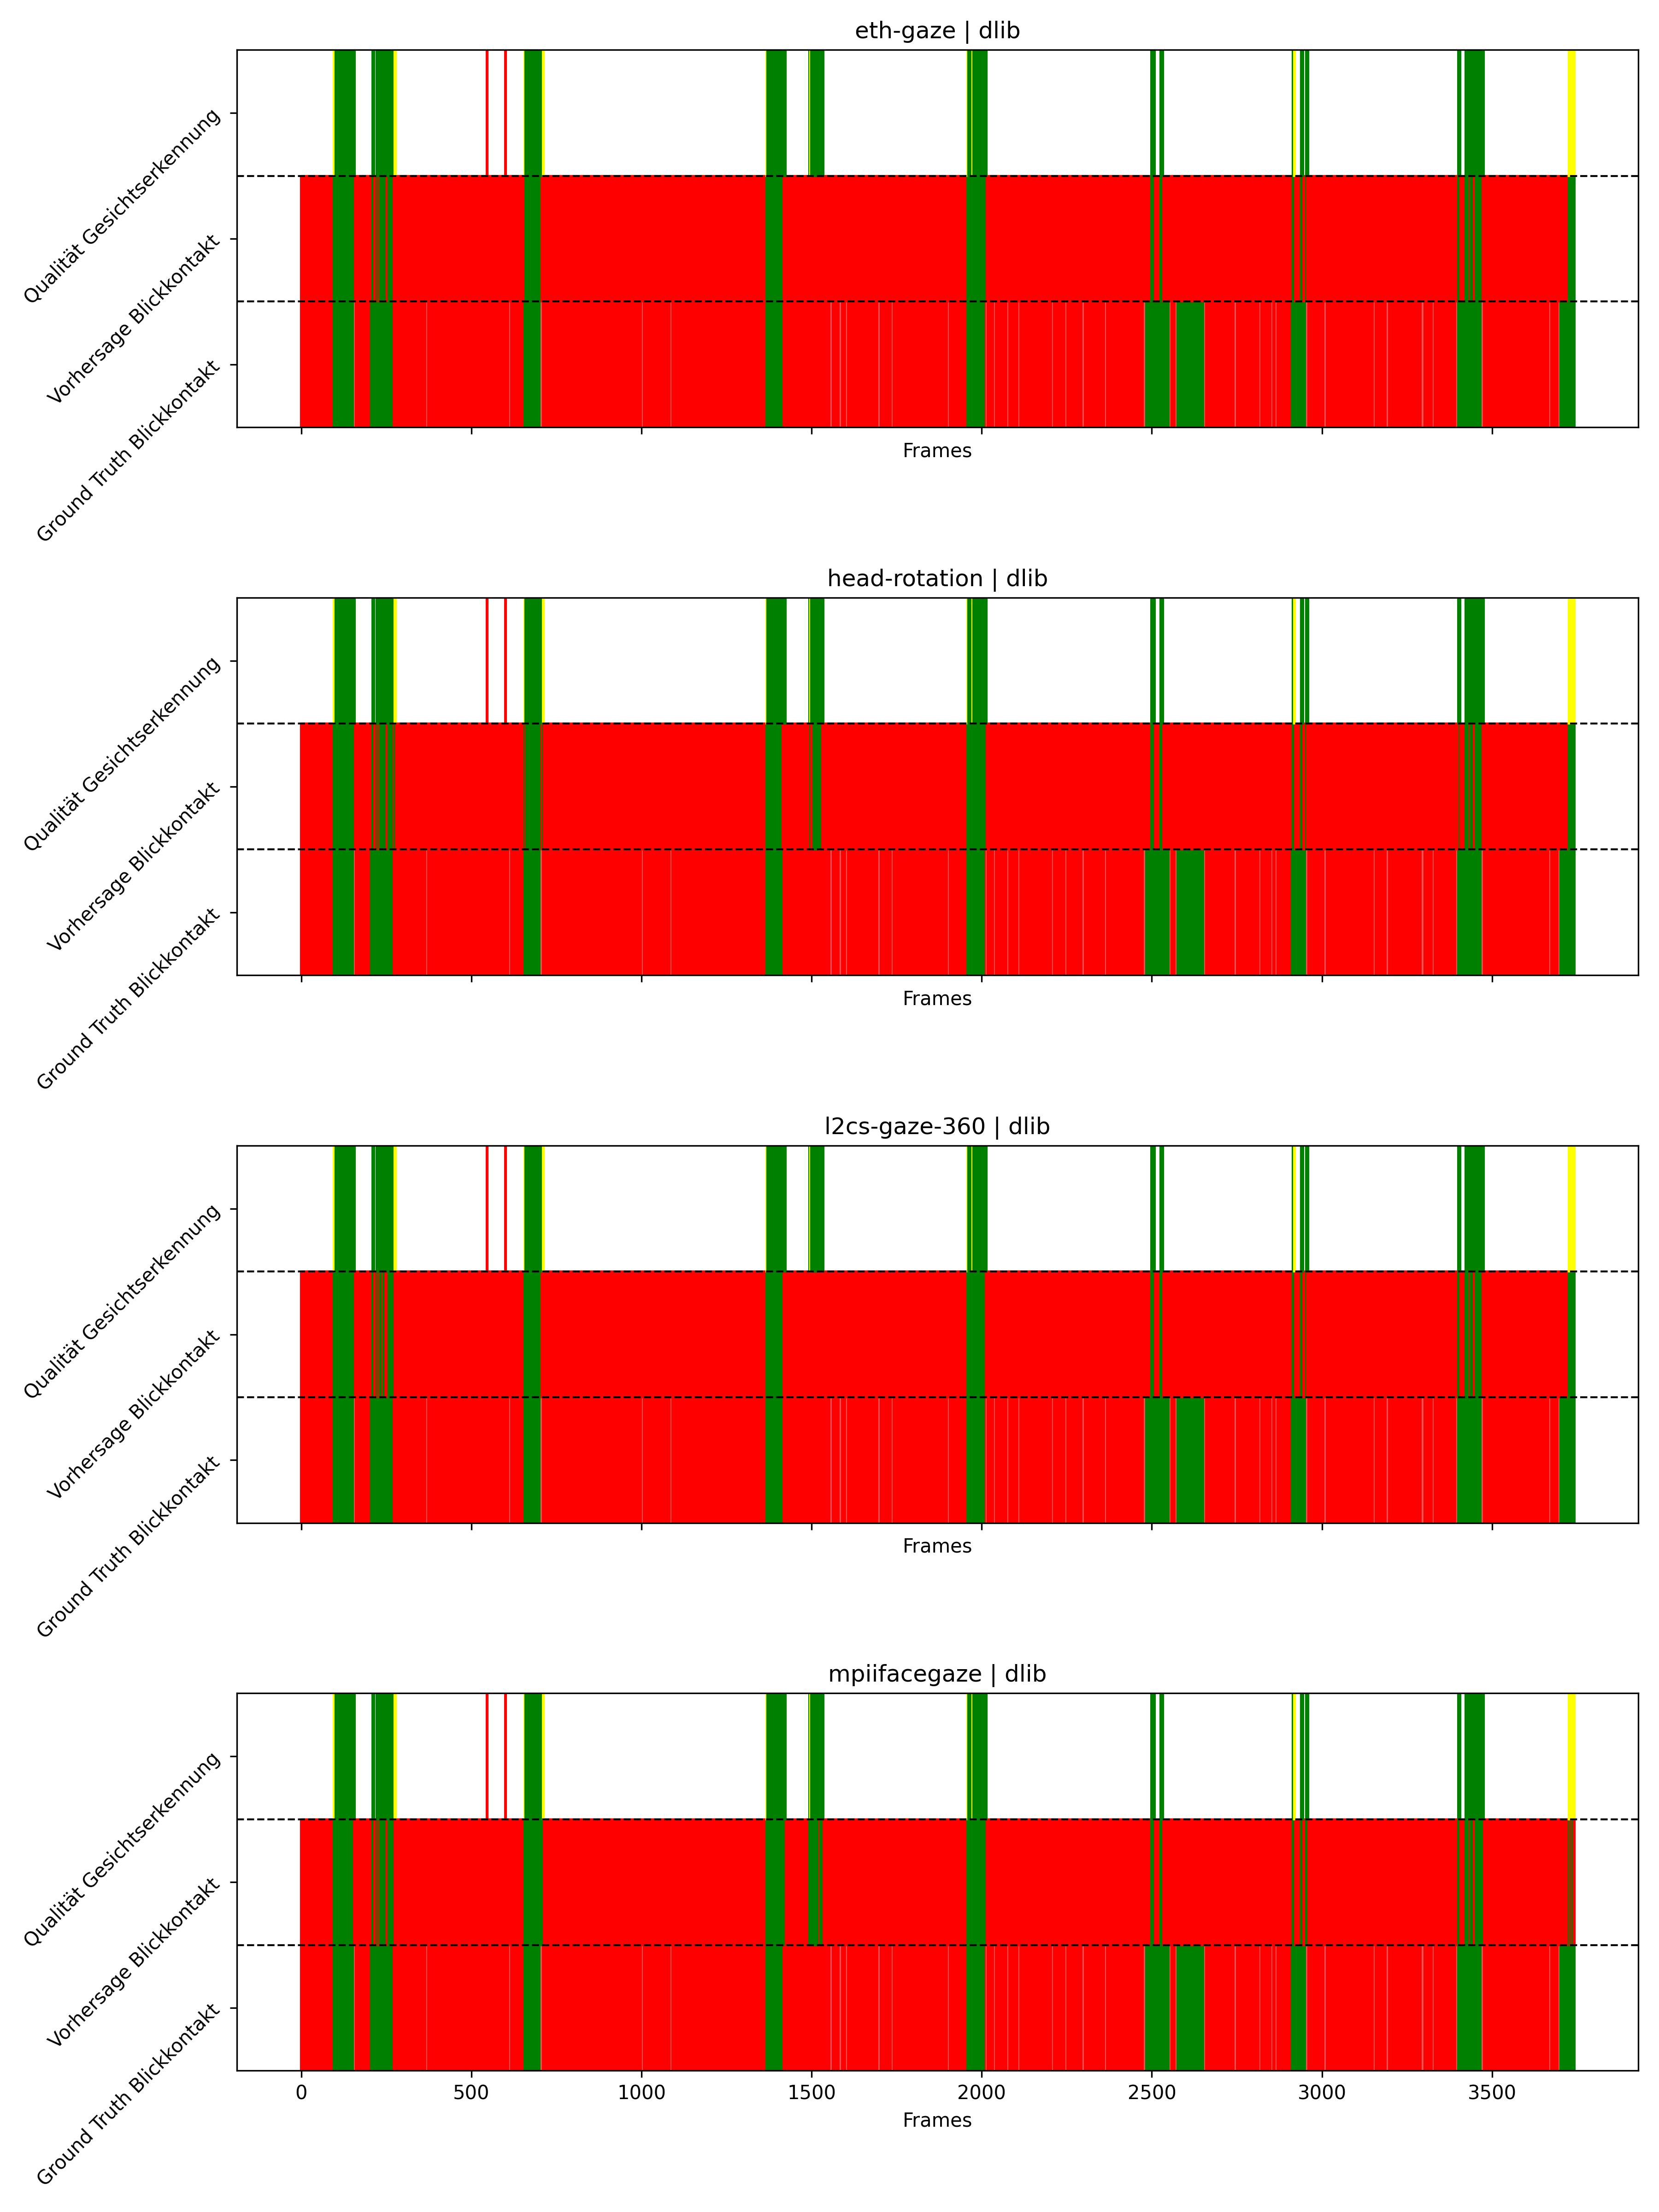
\includegraphics[width=1\linewidth]{appendix/14-dlib-overview-gaze.jpg}
\caption{Überblick über die Ground Truth des Blickkontakts, die Vorhersage des Blickkontakts und die Qualität der Gesichtserkennung mit \dlib. Die Bedeutung der Farben ist in Abbildung \ref{fig:evaluation:gaze:mpiifacegaze} erklärt.  }
\end{figure}

\begin{figure}[H]
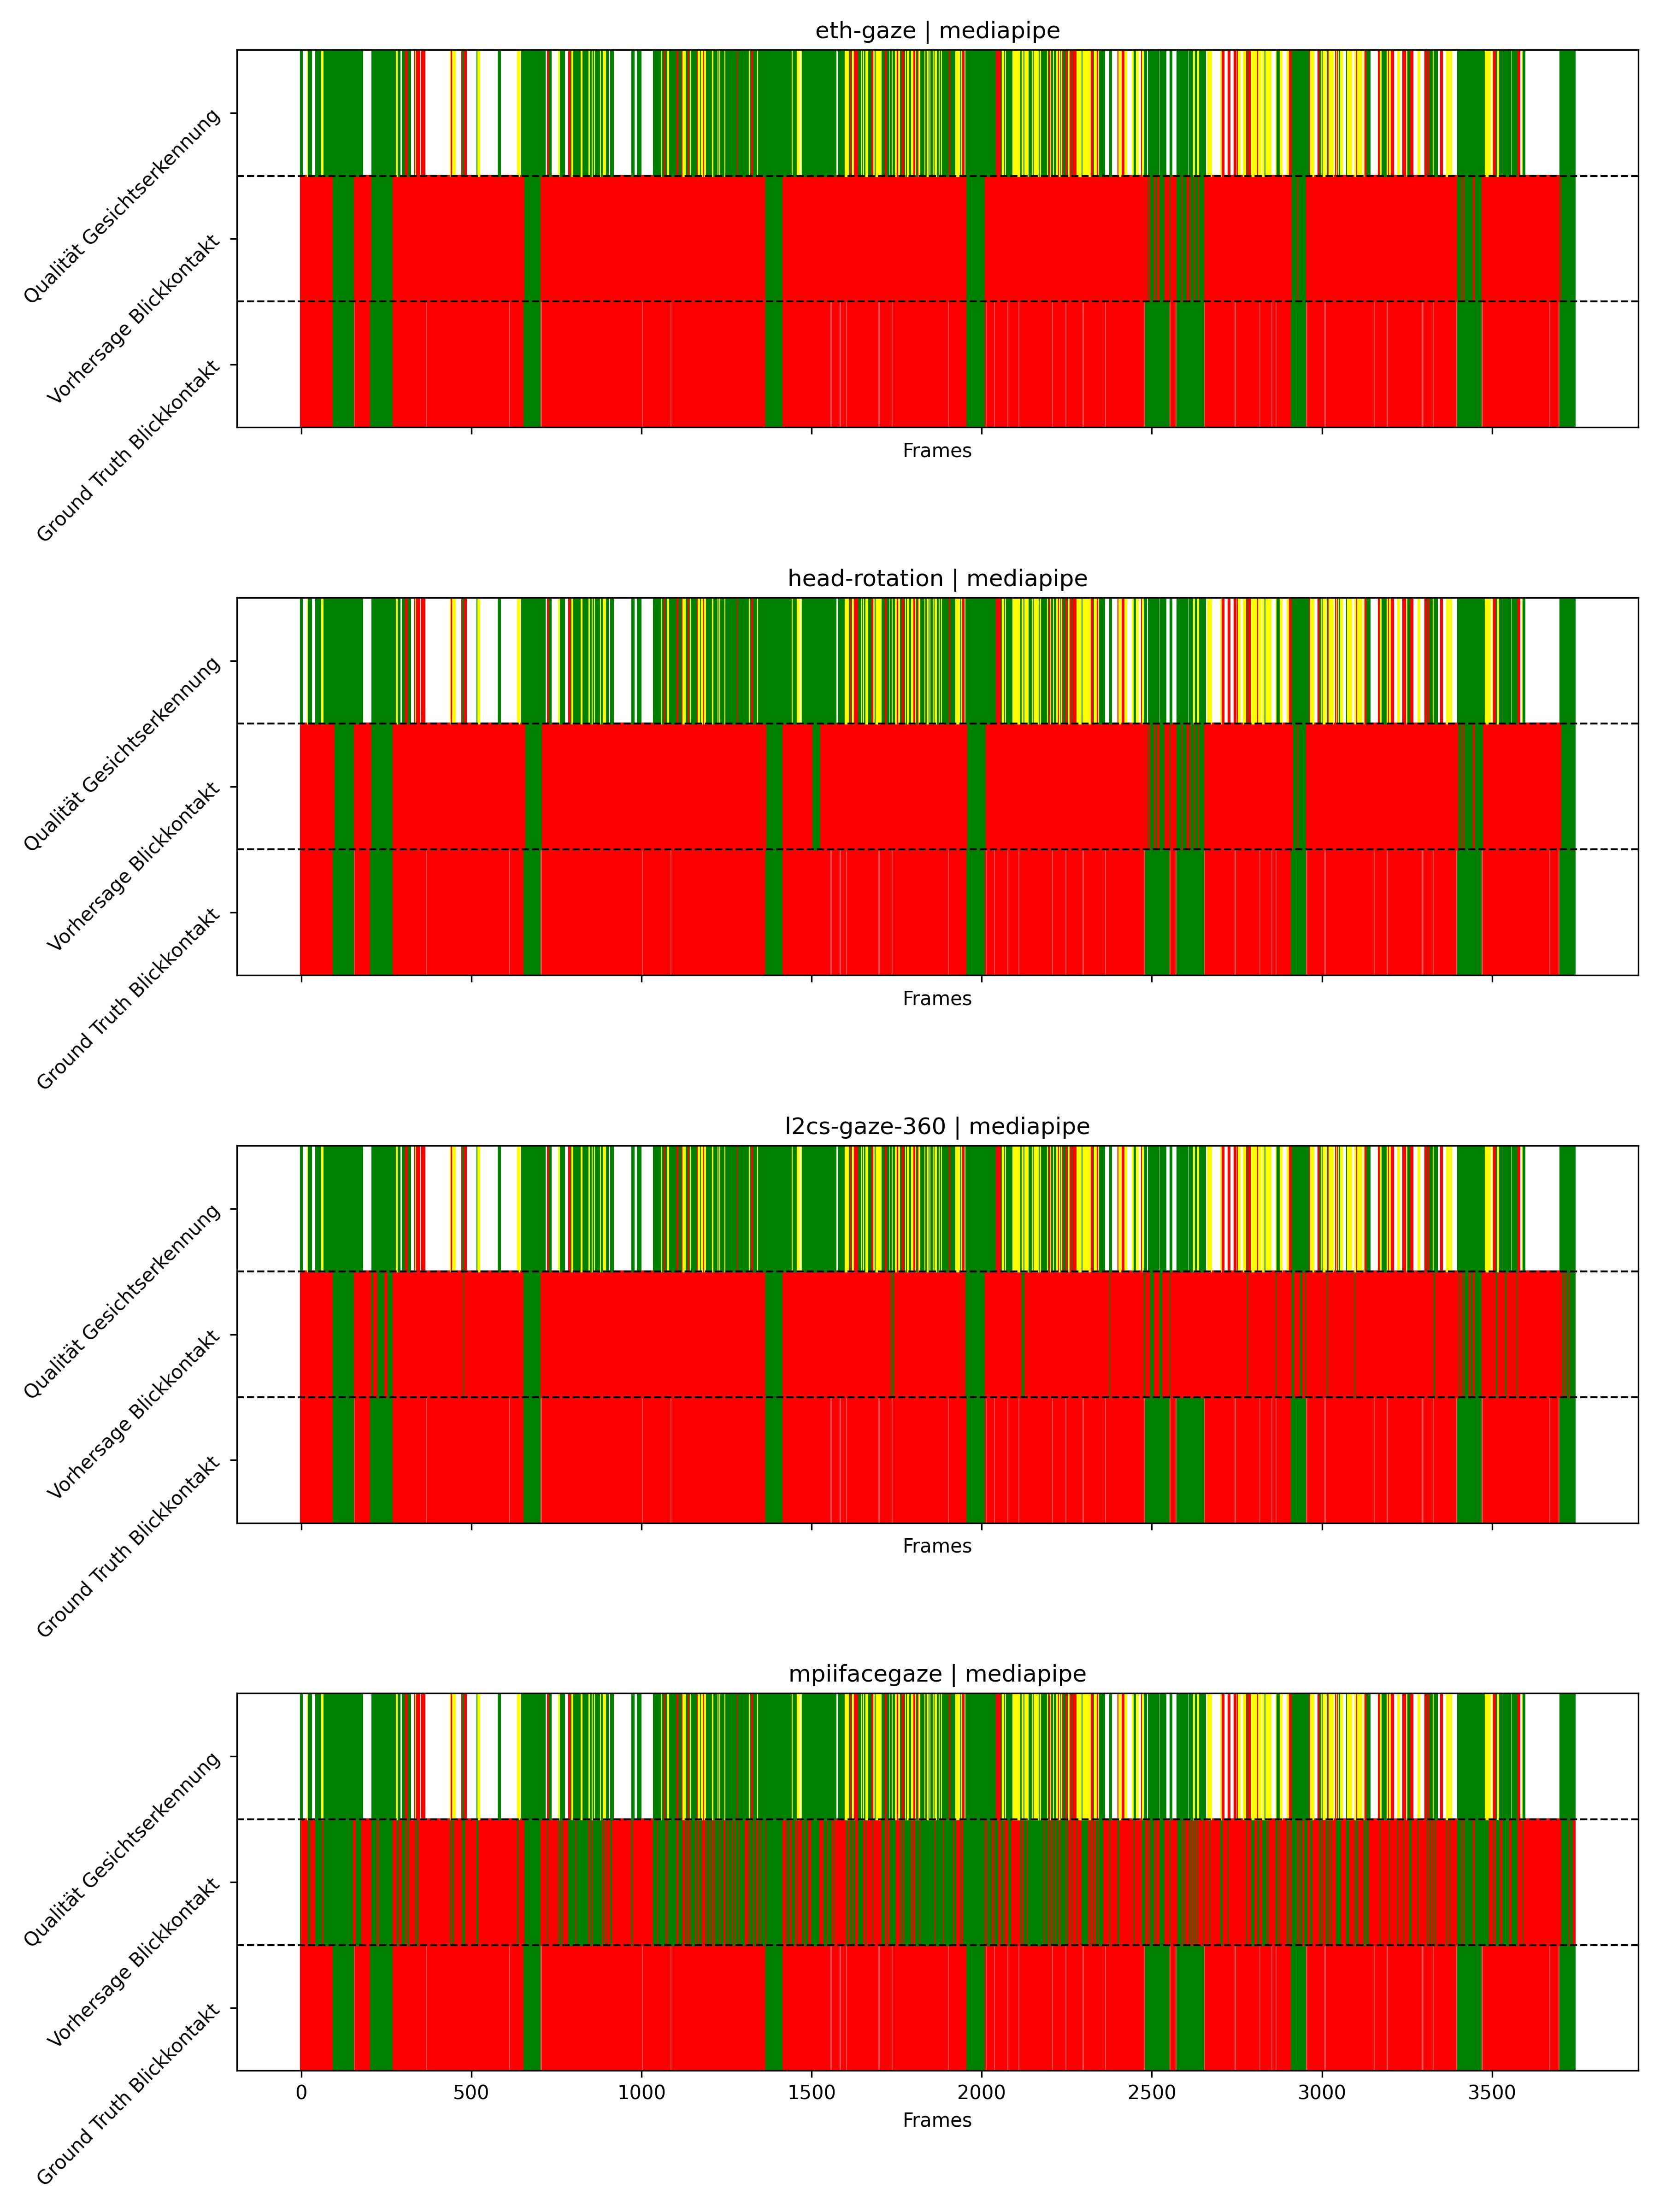
\includegraphics[width=1\linewidth]{appendix/14-mediapipe-overview-gaze.jpg}
\caption{Überblick über die Ground Truth des Blickkontakts, die Vorhersage des Blickkontakts und die Qualität der Gesichtserkennung mit \mediapipe. Die Bedeutung der Farben ist in Abbildung \ref{fig:evaluation:gaze:mpiifacegaze} erklärt.}
\end{figure}

\section{Video 15}
\begin{figure}[H]
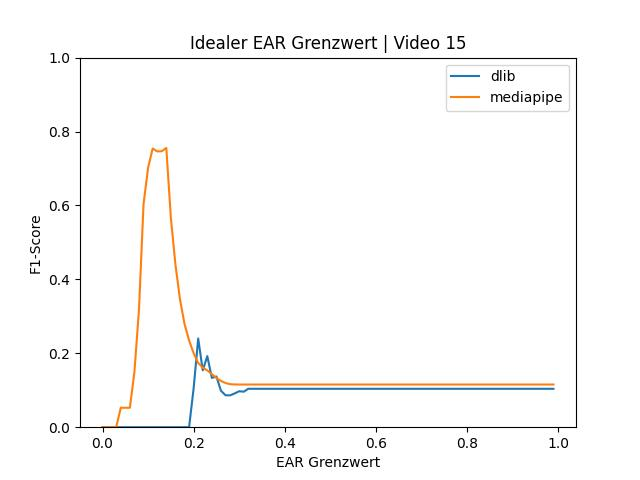
\includegraphics[width=0.7\linewidth]{appendix/15_f1-score-blink.jpg}
\caption{Ergebnisse der Bestimmung des idealen EAR-Grenzwerts für Video 15.}
\end{figure}

\begin{figure}[H]
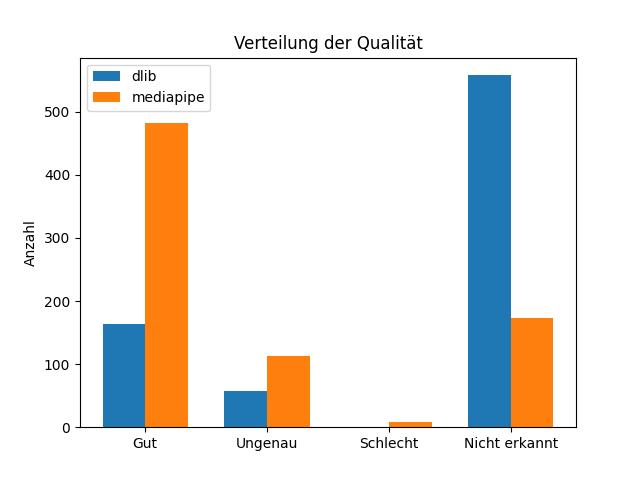
\includegraphics[width=0.7\linewidth]{appendix/15_bar-quality.jpg}
\caption{Aufteilung der Gesichtserkennungsqualität von Video 15.}
\end{figure}

\begin{table}[H]
\centering
\begin{tabular}{l|l|c c |c}
\toprule
\textbf{Gesichtserkennung} & \textbf{Blickrichtung} & \textbf{Seitenlänge} $\hitthresholdsize$ & \textbf{Verschiebung} $\hitthresholdposition$ & \textbf{F1-Score} \\ 
\midrule
\multirow{4}*{dlib}& ETH-XGaze & 0,133 & 0,01 & 0,988  \\ 
& Gaze360 & 0,5 & 0,047 & 0,945 \\ 
& MPIIFaceGaze & 0,102 & -0,027 & 0,893  \\ 
& Kopfrotation & 0,214 & 0,231 & 0,863  \\ 
\hline\multirow{4}*{MediaPipe}& ETH-XGaze & 0,133 & 0,01 & 0,988  \\ 
& Gaze360 & 0,5 & 0,047 & 0,929 \\ 
& MPIIFaceGaze & 0,071 & -0,039 & 0,62  \\ 
& Kopfrotation & 0,133 & 0,194 & 0,961  \\ 
\bottomrule\end{tabular}
\caption{Ergebnis des Hyperparameter-Tunings für die Zone speziell für Video 15.}
\label{tab:appendix:15:local}
\end{table}
\begin{table}[H]
\centering
\begin{tabular}{l|l|c c c c|c c|c}
\toprule
\textbf{Gesichtserkennung} & \textbf{Blickrichtung} & $TP$ & $TN$& $FP$ & $FN$ & \textbf{Precision} & \textbf{Recall} & \textbf{F1-Score} \\ 
\midrule
\multirow{4}*{dlib}& ETH-XGaze & 167 & 606 & 5 & 0 & 0,971 & 1,0 & 0,985 \\ 
& Gaze360 & 155 & 605 & 6 & 12 & 0,963 & 0,928 & 0,945 \\ 
& MPIIFaceGaze & 156 & 584 & 27 & 11 & 0,852 & 0,934 & 0,891 \\ 
& Kopfrotation & 166 & 558 & 53 & 1 & 0,758 & 0,994 & 0,86 \\ 
\hline\multirow{4}*{MediaPipe}& ETH-XGaze & 167 & 606 & 5 & 0 & 0,971 & 1,0 & 0,985 \\ 
& Gaze360 & 143 & 605 & 6 & 24 & 0,96 & 0,856 & 0,905 \\ 
& MPIIFaceGaze & 99 & 396 & 215 & 68 & 0,315 & 0,593 & 0,412 \\ 
& Kopfrotation & 162 & 600 & 11 & 5 & 0,936 & 0,97 & 0,953 \\ 
\bottomrule\end{tabular}
\caption{Zusammensetzung des F1-Scores unter Verwendung der in Kapitel \ref{sec:evaluation:results:gaze:threshold} bestimmten globalen Parameter $\hitthresholdsize$ und $\hitthresholdposition$.}
\label{tab:appendix:15:f1}
\end{table}
\begin{figure}[H]
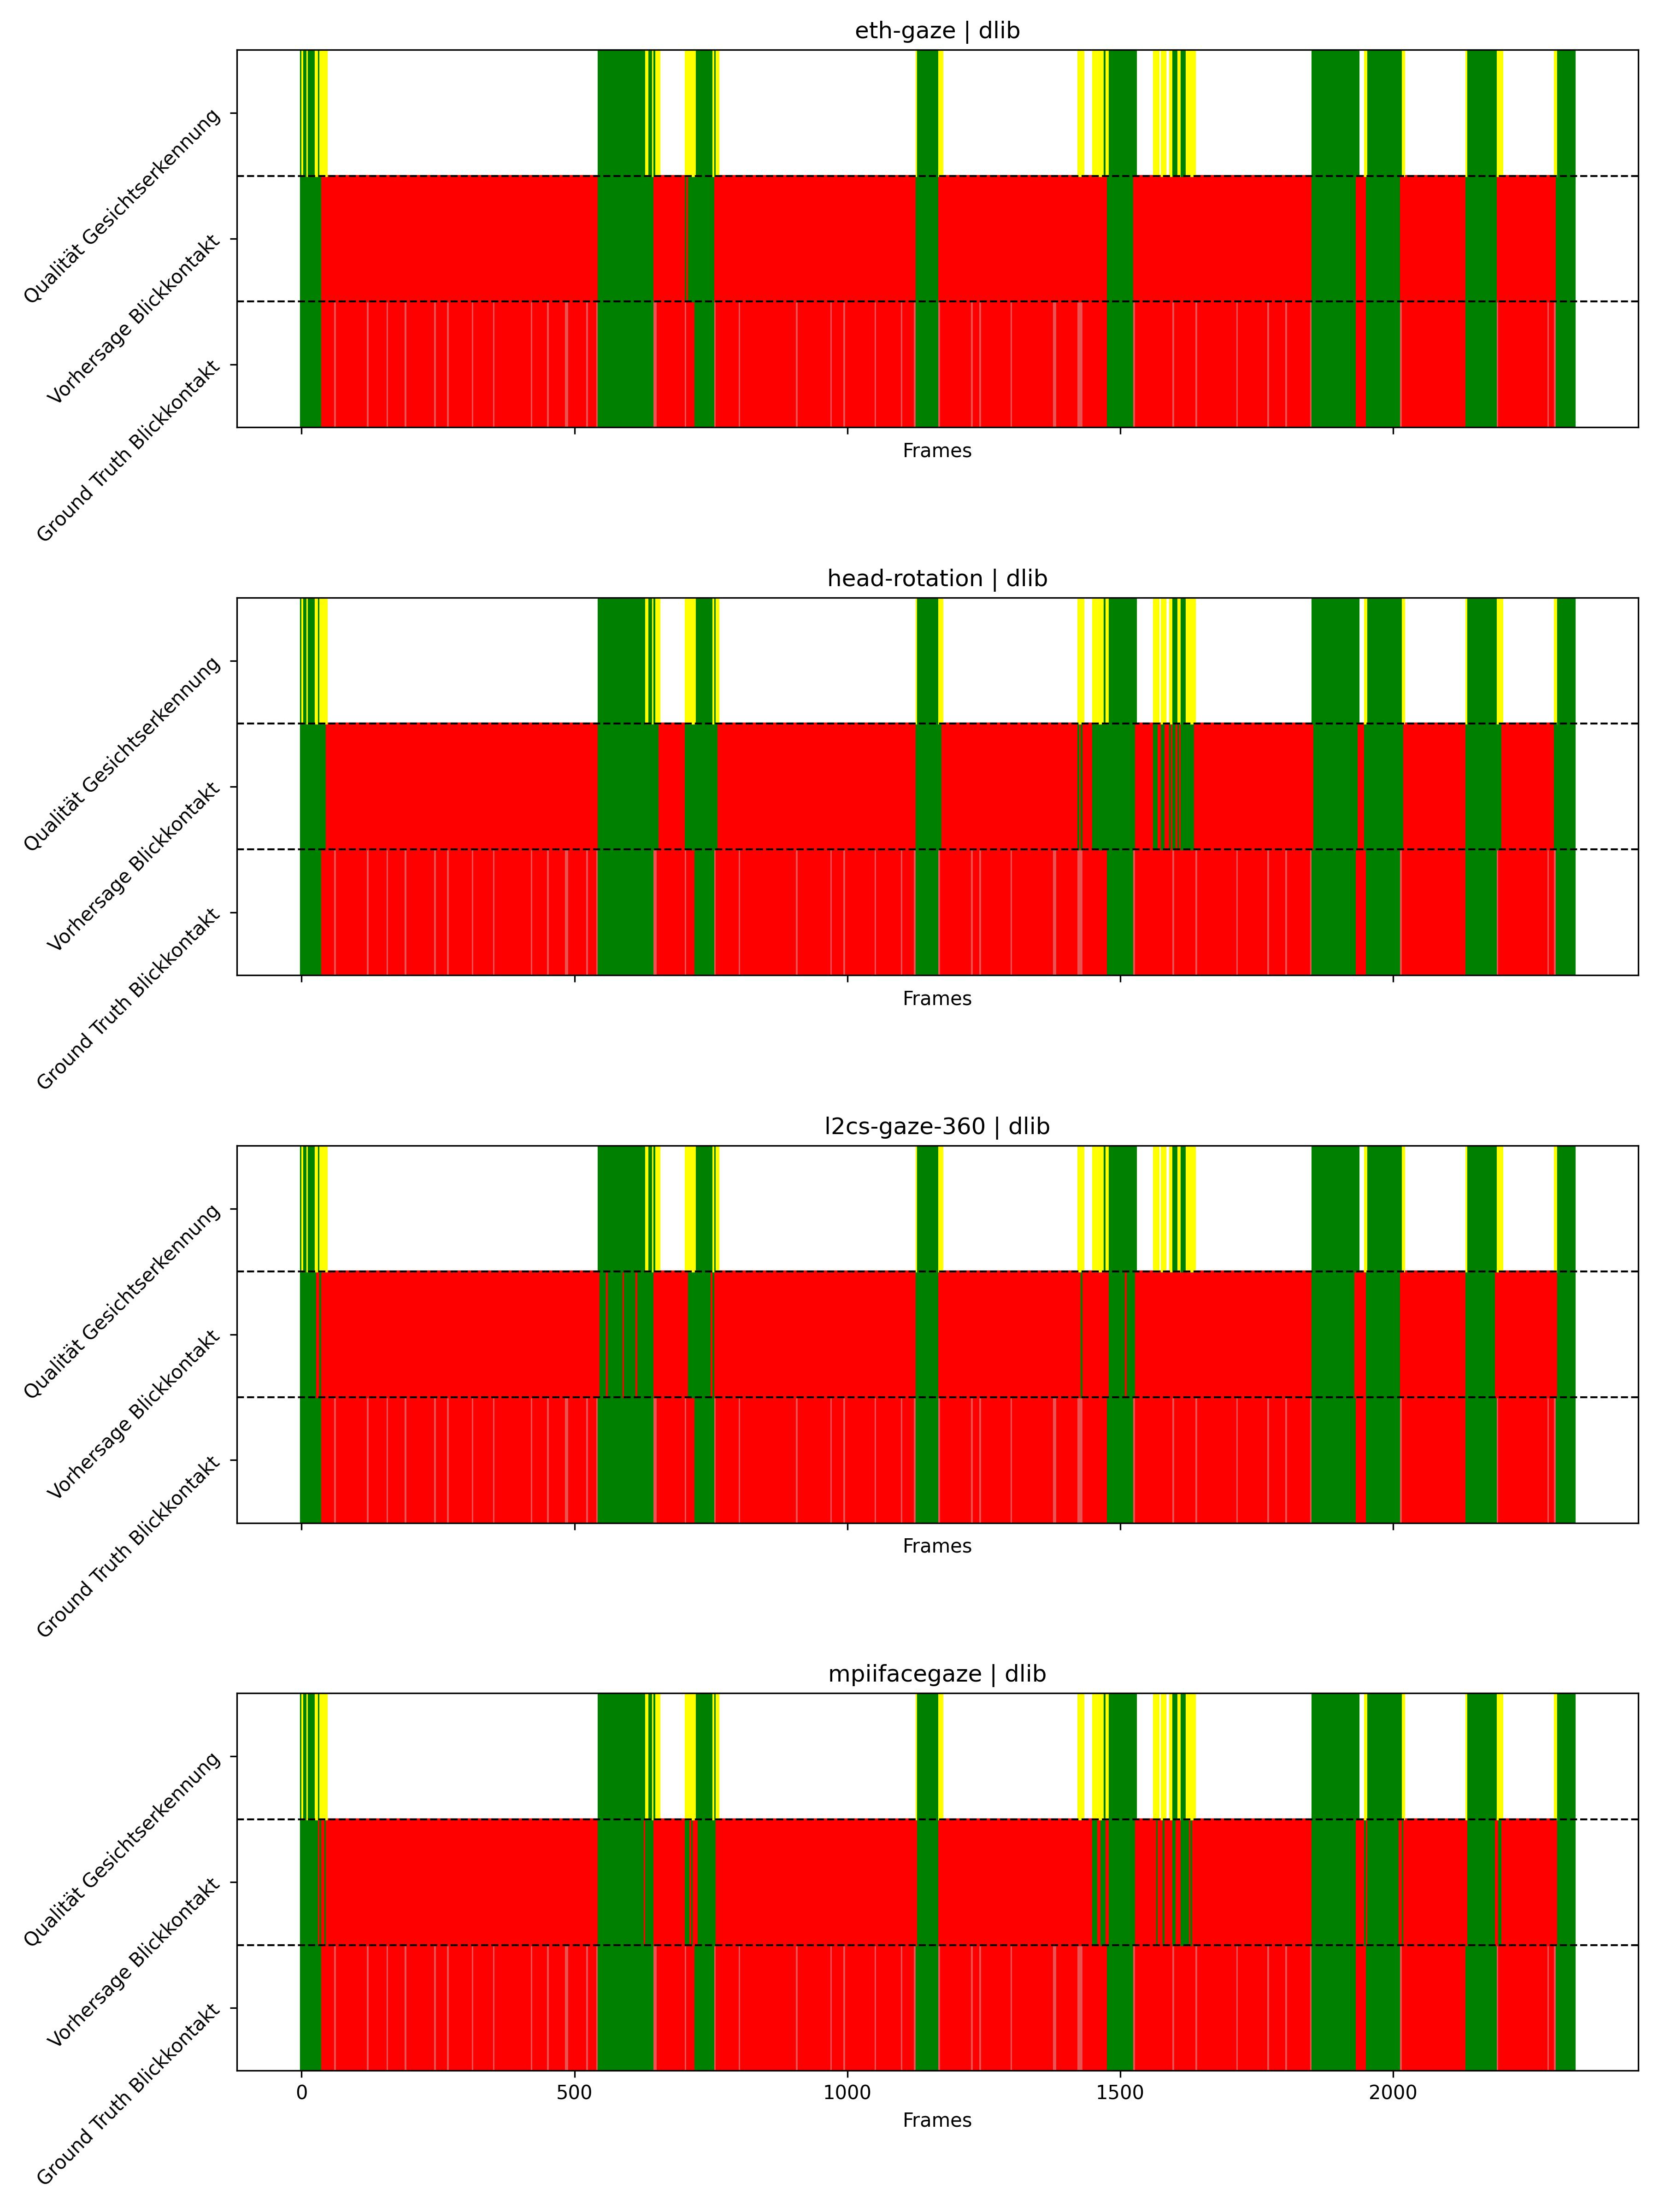
\includegraphics[width=1\linewidth]{appendix/15-dlib-overview-gaze.jpg}
\caption{Überblick über die Ground Truth des Blickkontakts, die Vorhersage des Blickkontakts und die Qualität der Gesichtserkennung mit \dlib. Die Bedeutung der Farben ist in Abbildung \ref{fig:evaluation:gaze:mpiifacegaze} erklärt.  }
\end{figure}

\begin{figure}[H]
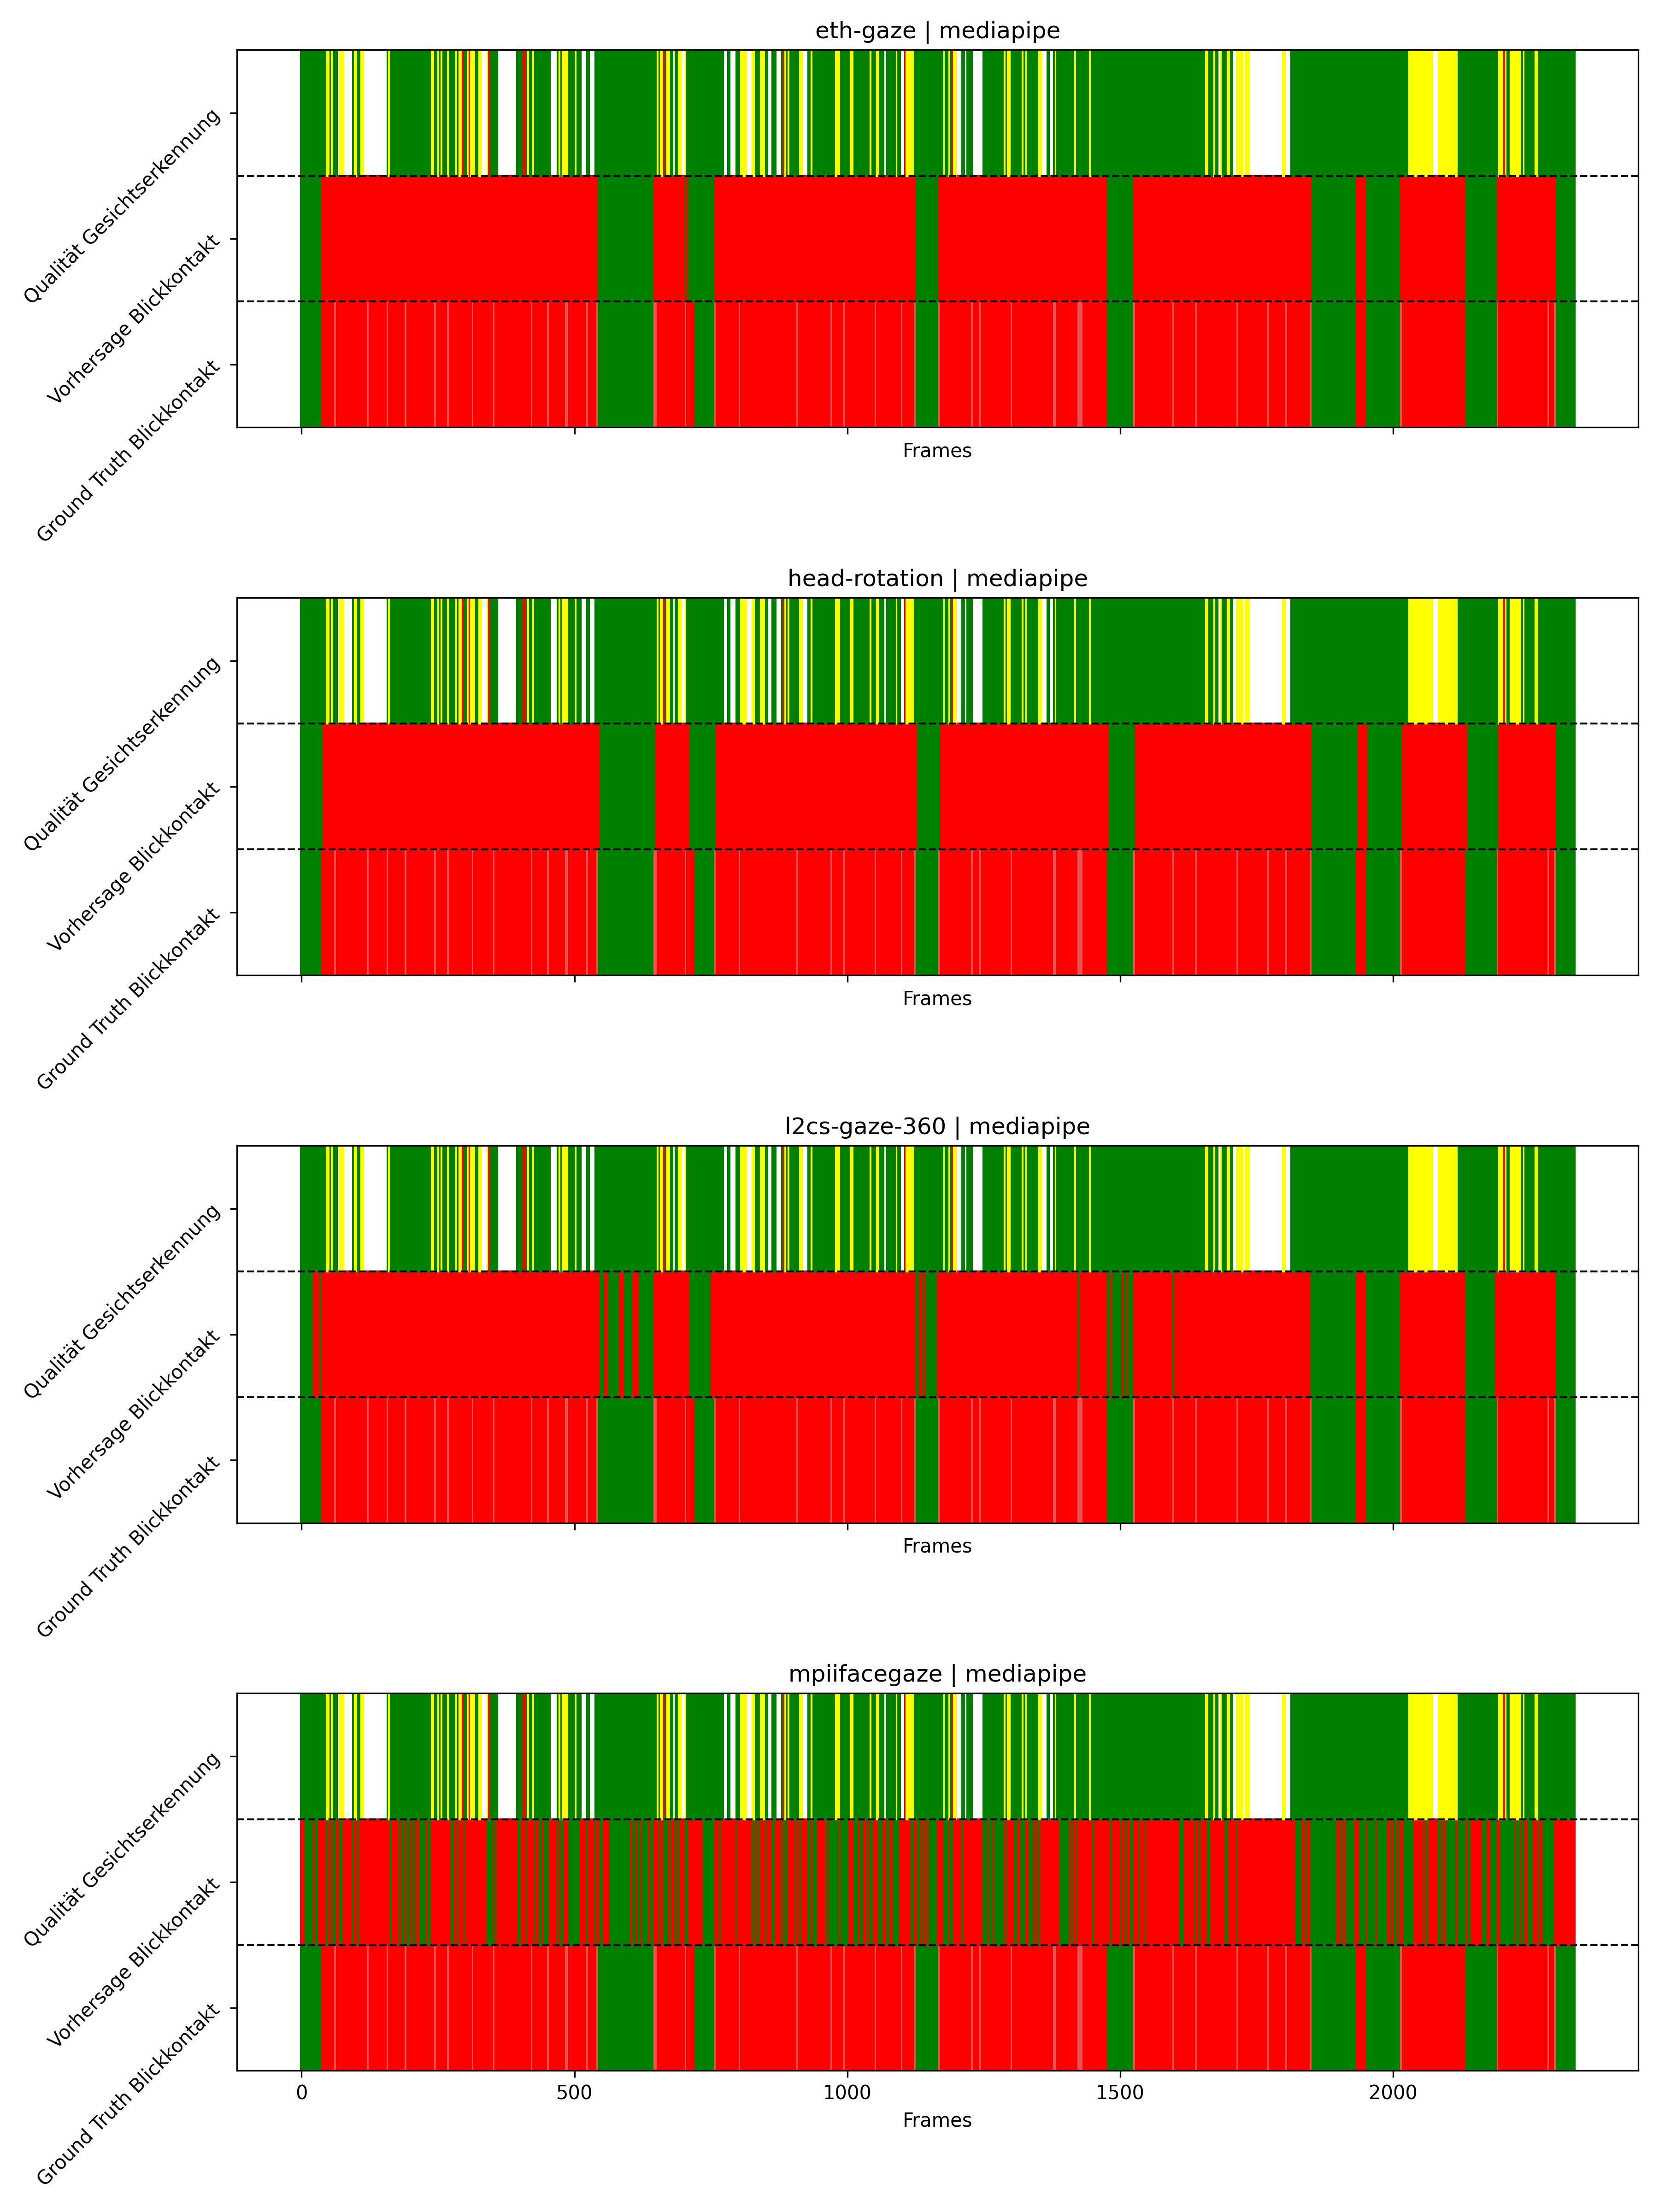
\includegraphics[width=1\linewidth]{appendix/15-mediapipe-overview-gaze.jpg}
\caption{Überblick über die Ground Truth des Blickkontakts, die Vorhersage des Blickkontakts und die Qualität der Gesichtserkennung mit \mediapipe. Die Bedeutung der Farben ist in Abbildung \ref{fig:evaluation:gaze:mpiifacegaze} erklärt.}
\end{figure}

\section{Video 16}
\begin{figure}[H]
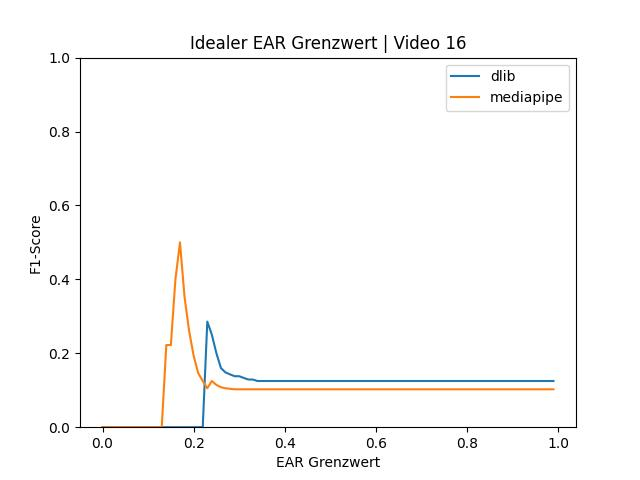
\includegraphics[width=0.7\linewidth]{appendix/16_f1-score-blink.jpg}
\caption{Ergebnisse der Bestimmung des idealen EAR-Grenzwerts für Video 16.}
\end{figure}

\begin{figure}[H]
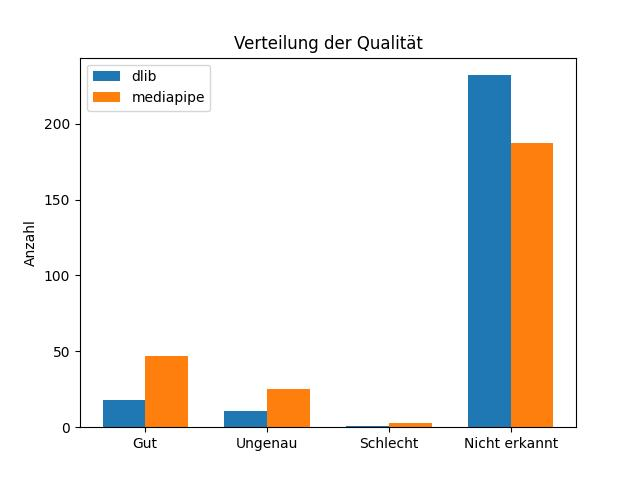
\includegraphics[width=0.7\linewidth]{appendix/16_bar-quality.jpg}
\caption{Aufteilung der Gesichtserkennungsqualität von Video 16.}
\end{figure}

\begin{table}[H]
\centering
\begin{tabular}{l|l|c c |c}
\toprule
\textbf{Gesichtserkennung} & \textbf{Blickrichtung} & \textbf{Seitenlänge} $\hitthresholdsize$ & \textbf{Verschiebung} $\hitthresholdposition$ & \textbf{F1-Score} \\ 
\midrule
\multirow{4}*{dlib}& ETH-XGaze & 0,133 & -0,002 & 1,0  \\ 
& Gaze360 & 0,245 & 0,059 & 0,976 \\ 
& MPIIFaceGaze & 0,071 & -0,014 & 0,864  \\ 
& Kopfrotation & 0,184 & 0,169 & 0,864  \\ 
\hline\multirow{4}*{MediaPipe}& ETH-XGaze & 0,112 & -0,014 & 1,0  \\ 
& Gaze360 & 0,347 & 0,059 & 0,952 \\ 
& MPIIFaceGaze & 0,102 & 0,047 & 0,507  \\ 
& Kopfrotation & 0,276 & 0,194 & 0,974  \\ 
\bottomrule\end{tabular}
\caption{Ergebnis des Hyperparameter-Tunings für die Zone speziell für Video 16.}
\label{tab:appendix:16:local}
\end{table}
\begin{table}[H]
\centering
\begin{tabular}{l|l|c c c c|c c|c}
\toprule
\textbf{Gesichtserkennung} & \textbf{Blickrichtung} & $TP$ & $TN$& $FP$ & $FN$ & \textbf{Precision} & \textbf{Recall} & \textbf{F1-Score} \\ 
\midrule
\multirow{4}*{dlib}& ETH-XGaze & 20 & 240 & 1 & 0 & 0,952 & 1,0 & 0,976 \\ 
& Gaze360 & 19 & 238 & 3 & 1 & 0,864 & 0,95 & 0,905 \\ 
& MPIIFaceGaze & 18 & 236 & 5 & 2 & 0,783 & 0,9 & 0,837 \\ 
& Kopfrotation & 20 & 234 & 7 & 0 & 0,741 & 1,0 & 0,851 \\ 
\hline\multirow{4}*{MediaPipe}& ETH-XGaze & 20 & 240 & 2 & 0 & 0,909 & 1,0 & 0,952 \\ 
& Gaze360 & 19 & 240 & 2 & 1 & 0,905 & 0,95 & 0,927 \\ 
& MPIIFaceGaze & 16 & 209 & 33 & 4 & 0,327 & 0,8 & 0,464 \\ 
& Kopfrotation & 20 & 240 & 2 & 0 & 0,909 & 1,0 & 0,952 \\ 
\bottomrule\end{tabular}
\caption{Zusammensetzung des F1-Scores unter Verwendung der in Kapitel \ref{sec:evaluation:results:gaze:threshold} bestimmten globalen Parameter $\hitthresholdsize$ und $\hitthresholdposition$.}
\label{tab:appendix:16:f1}
\end{table}
\begin{figure}[H]
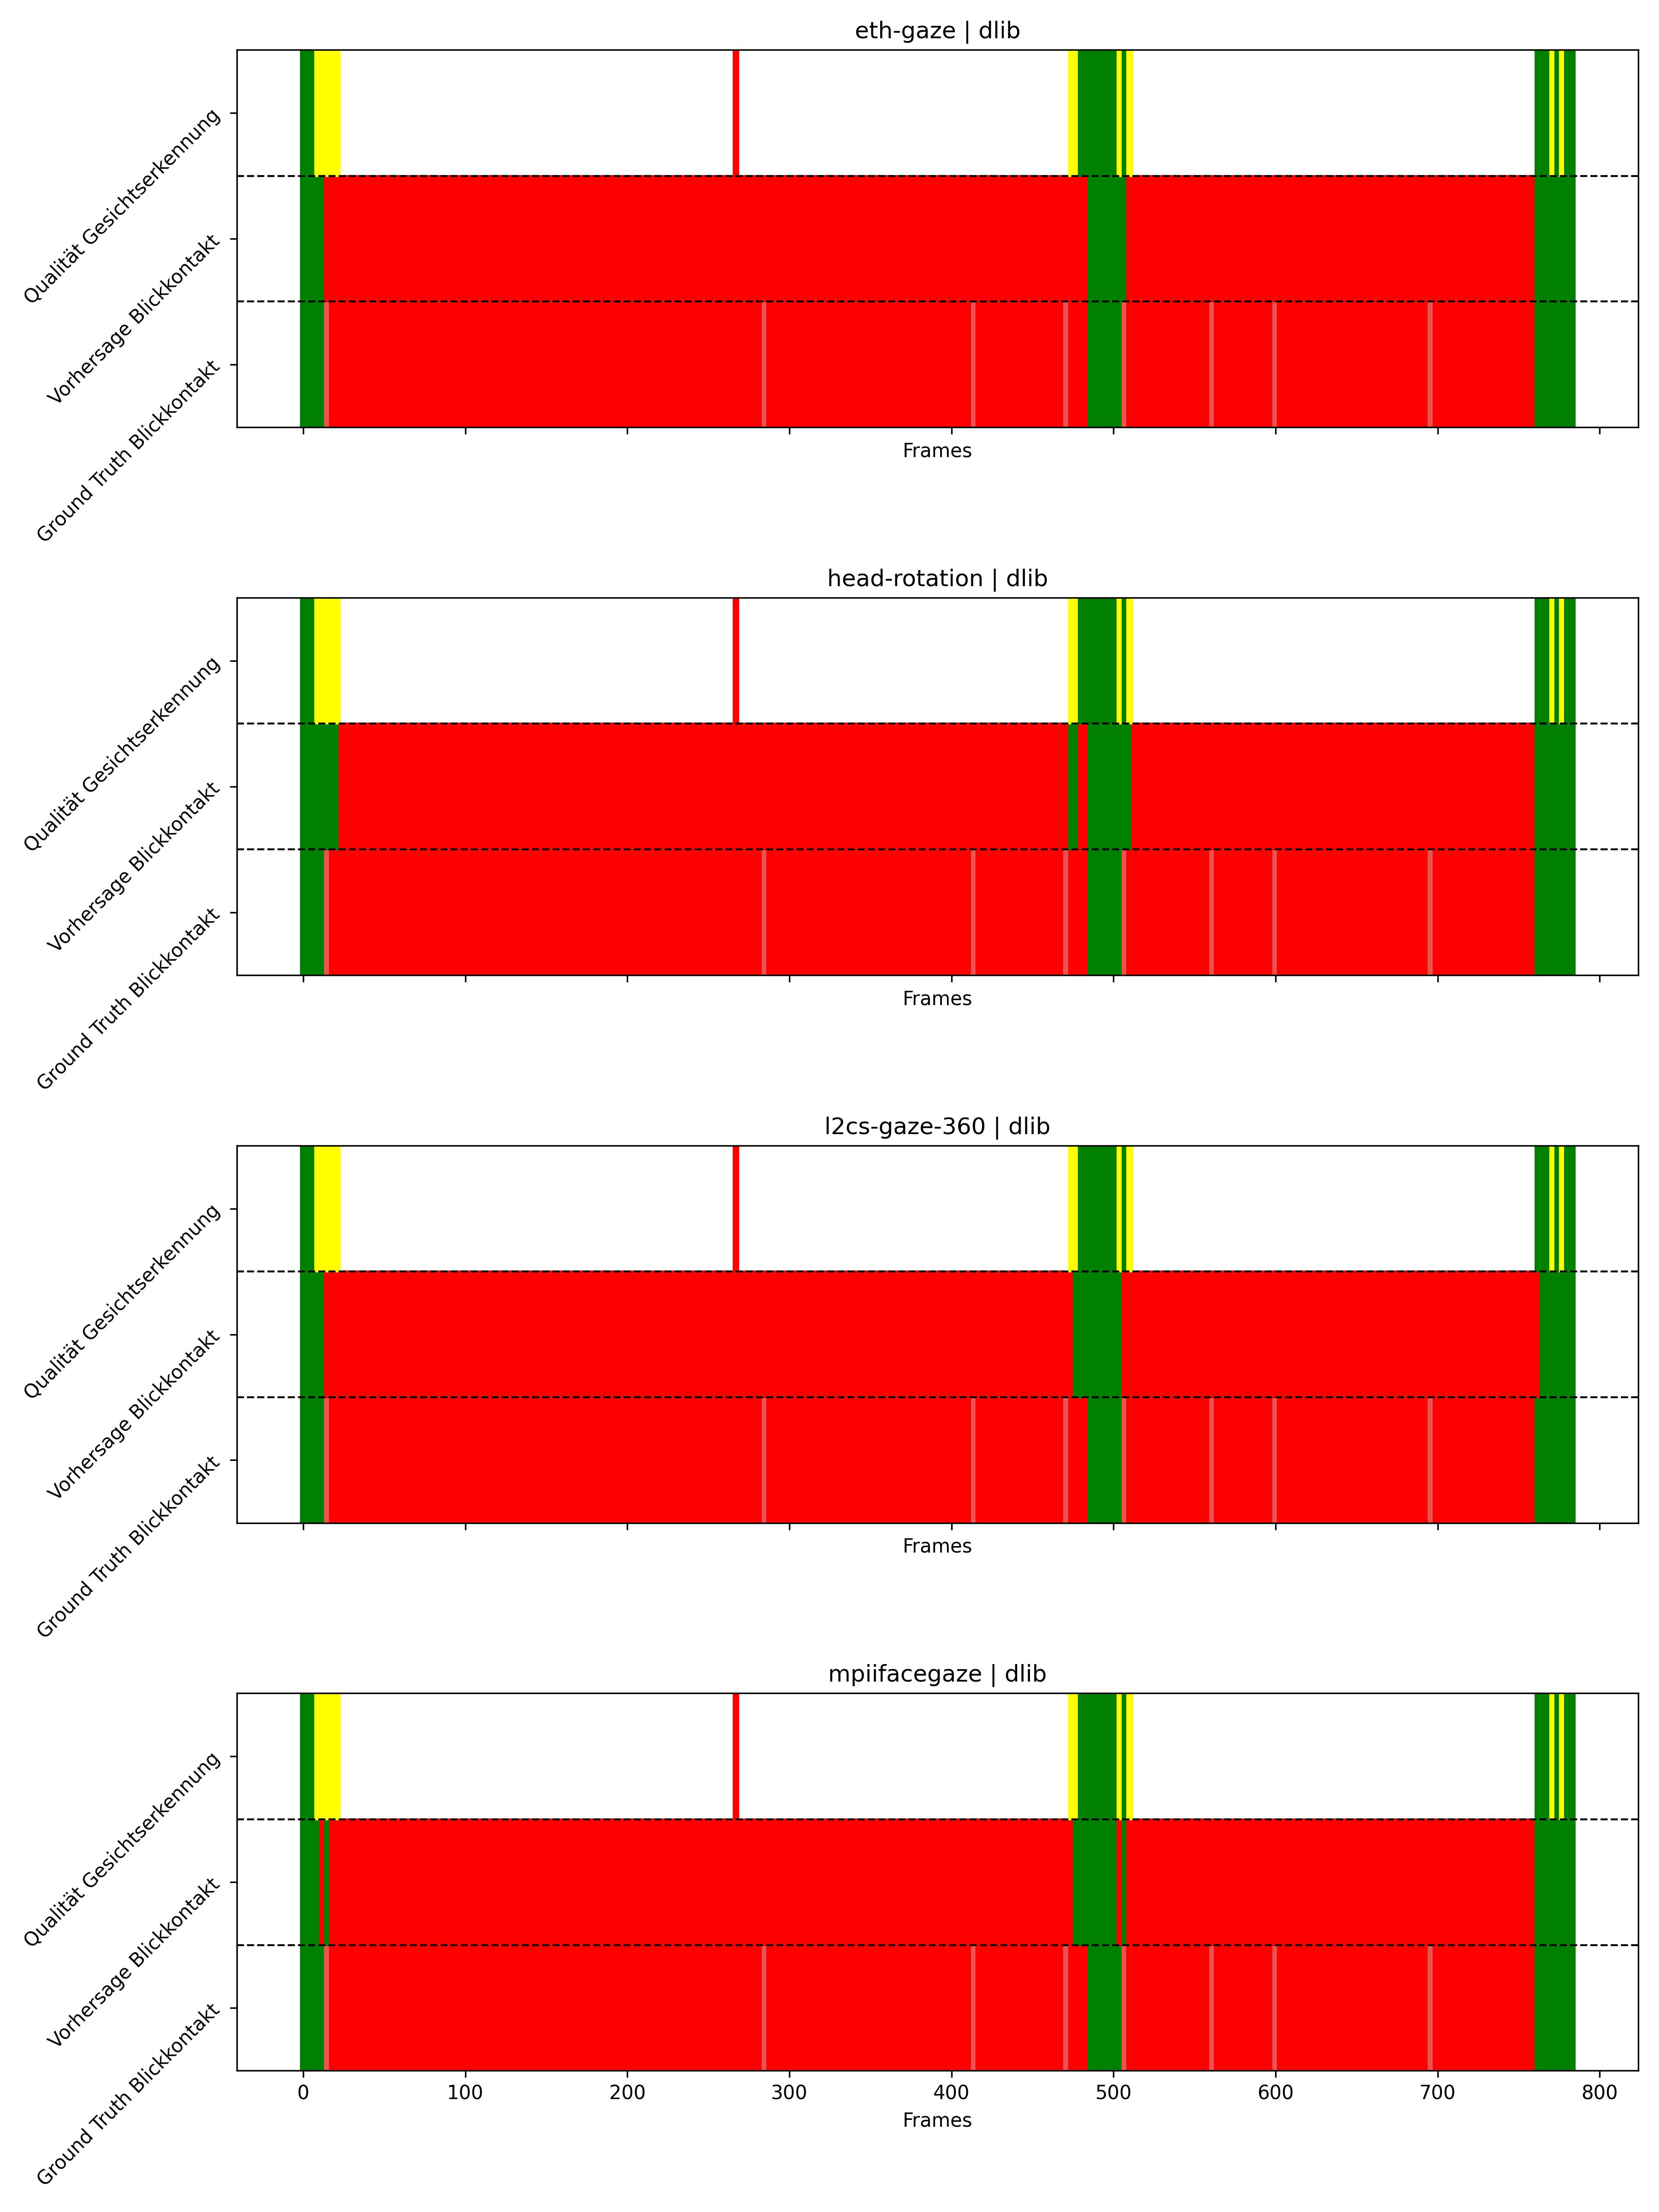
\includegraphics[width=1\linewidth]{appendix/16-dlib-overview-gaze.jpg}
\caption{Überblick über die Ground Truth des Blickkontakts, die Vorhersage des Blickkontakts und die Qualität der Gesichtserkennung mit \dlib. Die Bedeutung der Farben ist in Abbildung \ref{fig:evaluation:gaze:mpiifacegaze} erklärt.  }
\end{figure}

\begin{figure}[H]
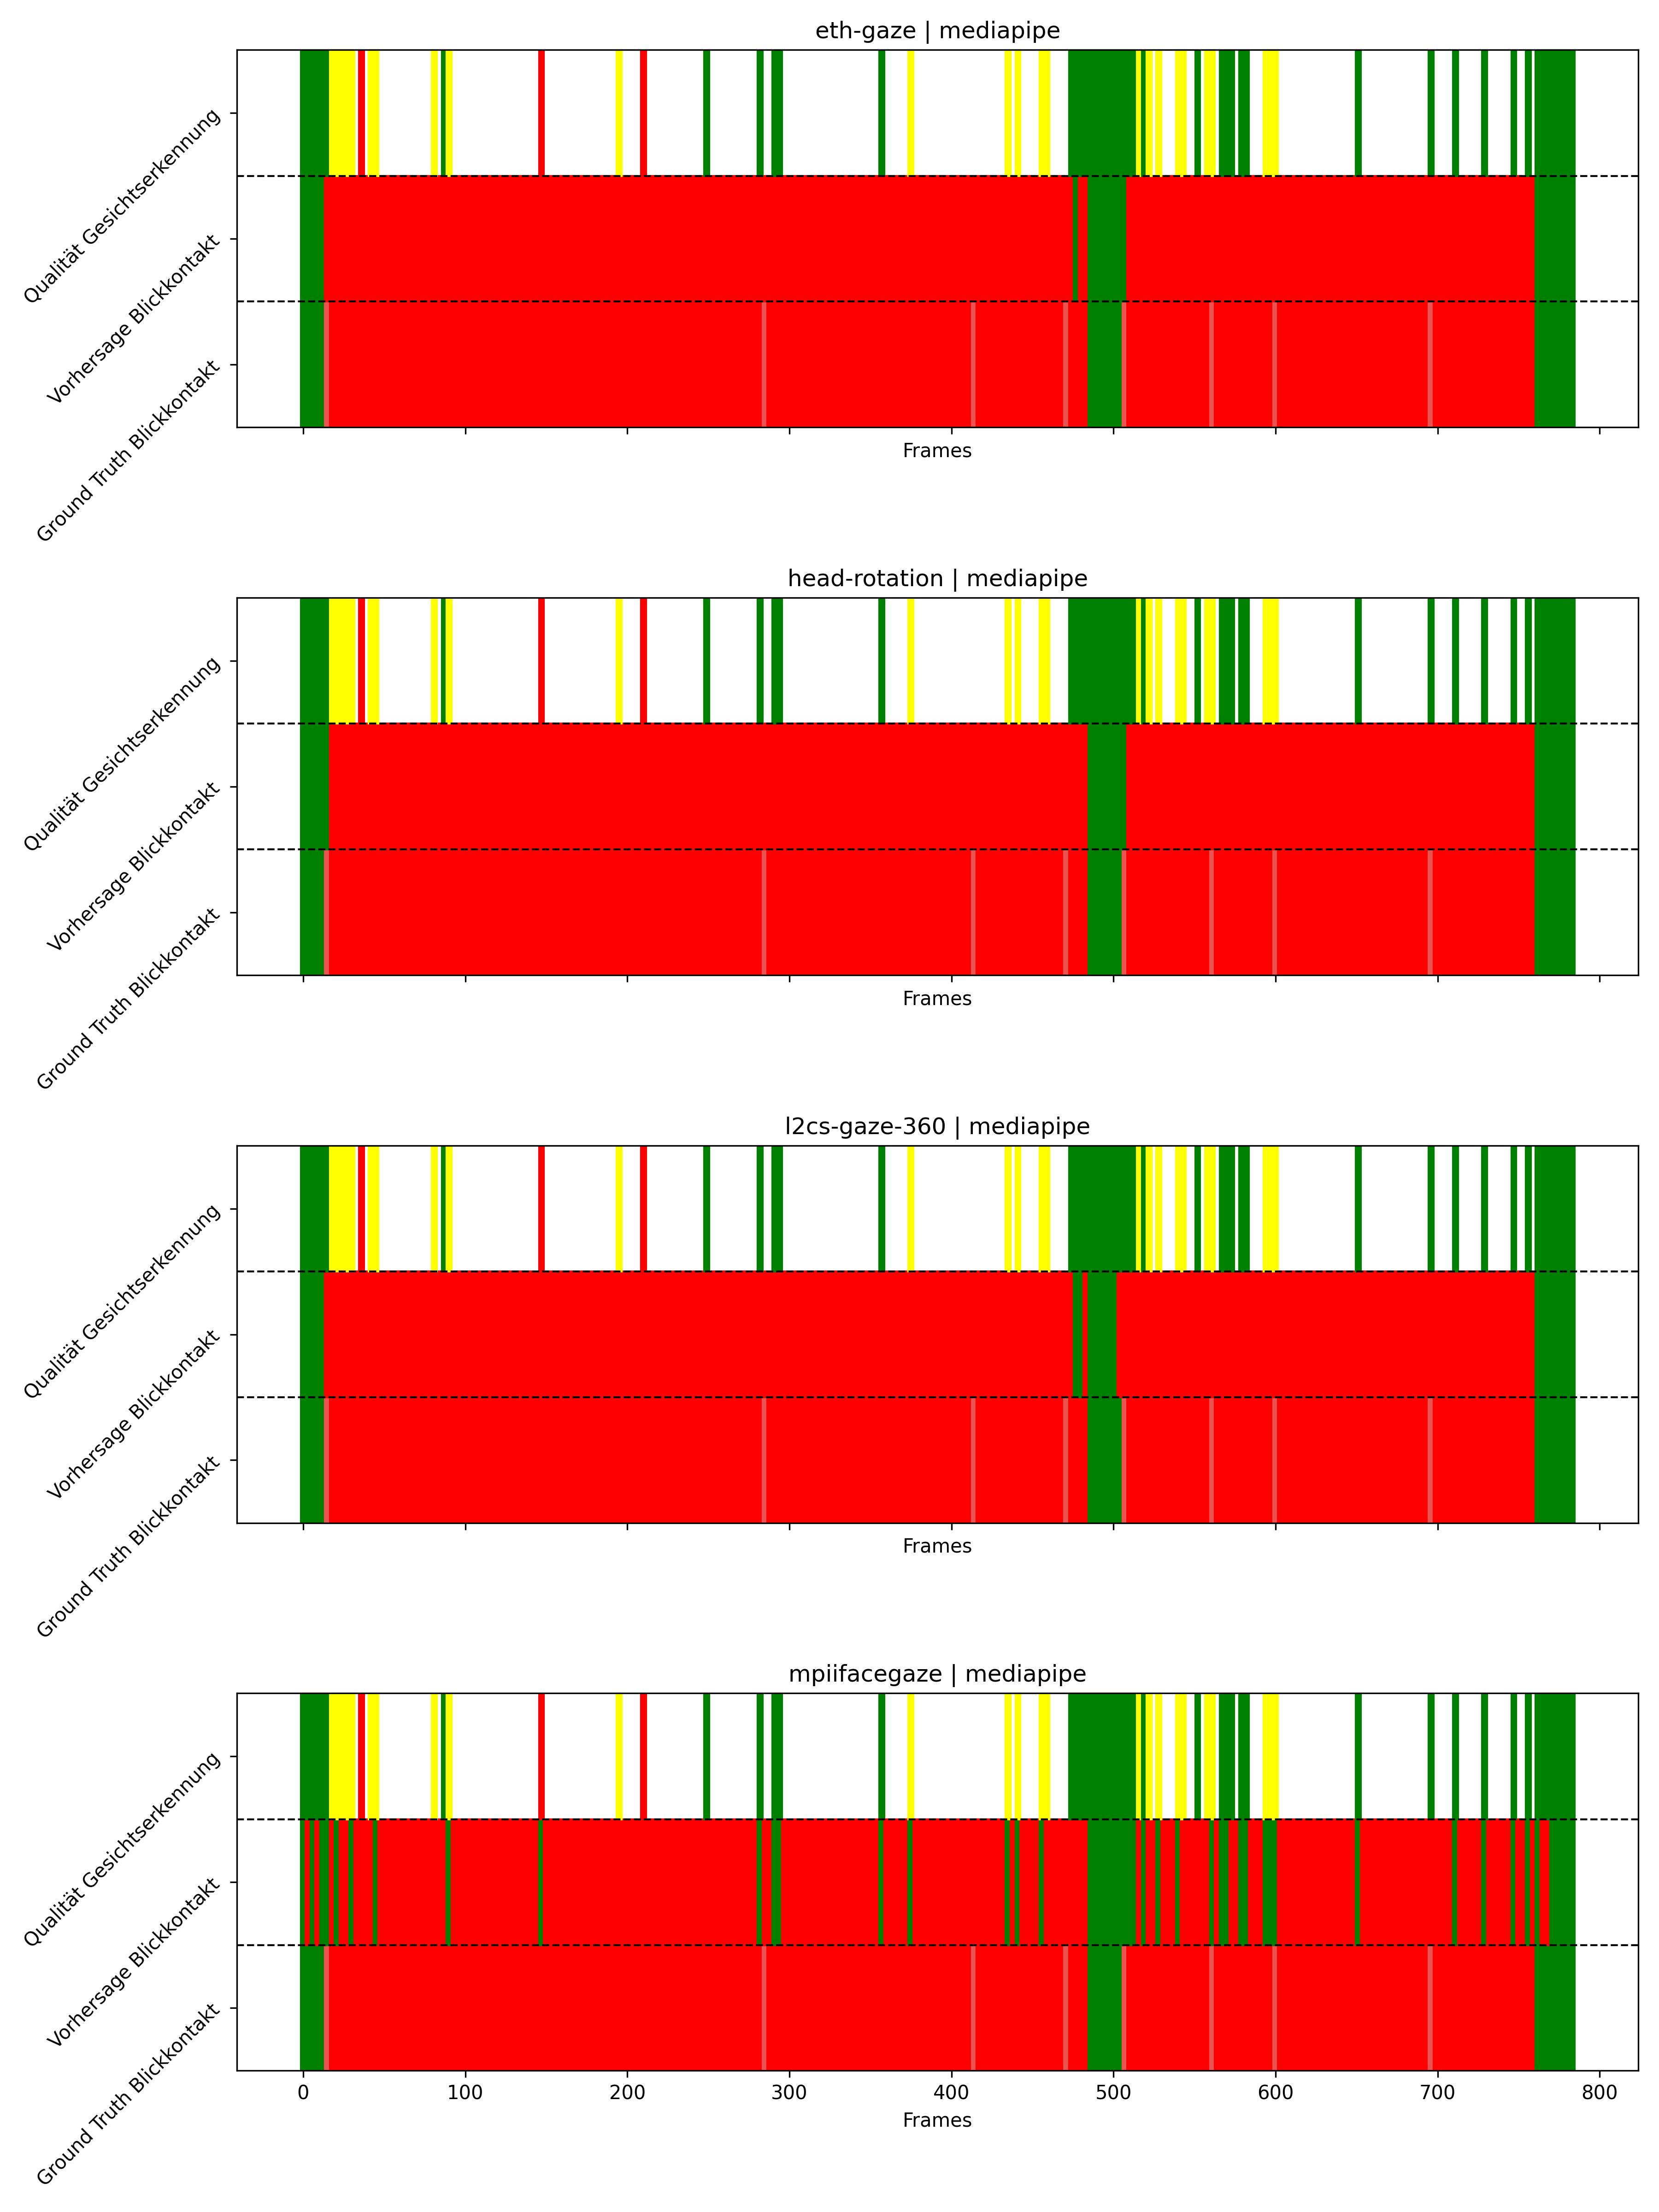
\includegraphics[width=1\linewidth]{appendix/16-mediapipe-overview-gaze.jpg}
\caption{Überblick über die Ground Truth des Blickkontakts, die Vorhersage des Blickkontakts und die Qualität der Gesichtserkennung mit \mediapipe. Die Bedeutung der Farben ist in Abbildung \ref{fig:evaluation:gaze:mpiifacegaze} erklärt.}
\end{figure}

\section{Video 17}
\begin{figure}[H]
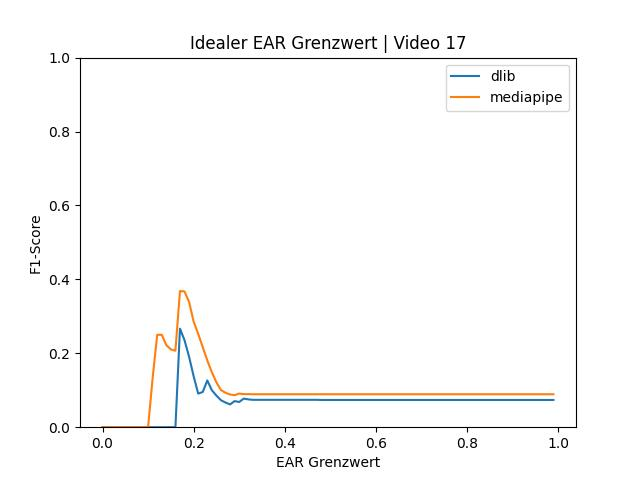
\includegraphics[width=0.7\linewidth]{appendix/17_f1-score-blink.jpg}
\caption{Ergebnisse der Bestimmung des idealen EAR-Grenzwerts für Video 17.}
\end{figure}

\begin{figure}[H]
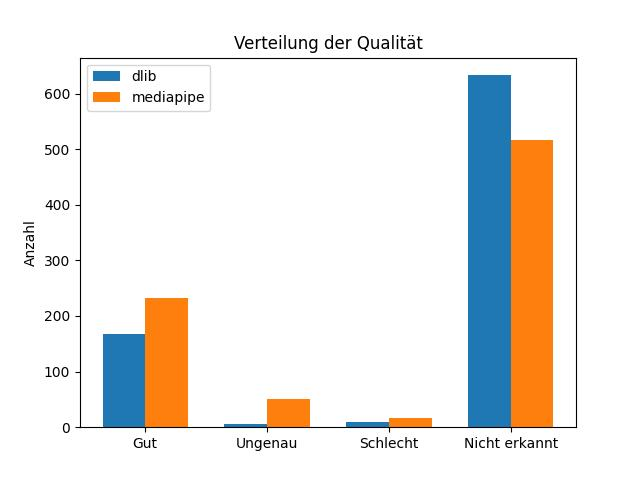
\includegraphics[width=0.7\linewidth]{appendix/17_bar-quality.jpg}
\caption{Aufteilung der Gesichtserkennungsqualität von Video 17.}
\end{figure}

\begin{table}[H]
\centering
\begin{tabular}{l|l|c c |c}
\toprule
\textbf{Gesichtserkennung} & \textbf{Blickrichtung} & \textbf{Seitenlänge} $\hitthresholdsize$ & \textbf{Verschiebung} $\hitthresholdposition$ & \textbf{F1-Score} \\ 
\midrule
\multirow{4}*{dlib}& ETH-XGaze & 0,173 & 0,047 & 0,869  \\ 
& Gaze360 & 0,48 & 0,427 & 0,838 \\ 
& MPIIFaceGaze & 0,051 & -0,027 & 0,881  \\ 
& Kopfrotation & 0,204 & 0,243 & 0,865  \\ 
\hline\multirow{4}*{MediaPipe}& ETH-XGaze & 0,153 & -0,002 & 0,918  \\ 
& Gaze360 & 0,49 & 0,451 & 0,804 \\ 
& MPIIFaceGaze & 0,051 & -0,039 & 0,838  \\ 
& Kopfrotation & 0,245 & 0,28 & 0,911  \\ 
\bottomrule\end{tabular}
\caption{Ergebnis des Hyperparameter-Tunings für die Zone speziell für Video 17.}
\label{tab:appendix:17:local}
\end{table}
\begin{table}[H]
\centering
\begin{tabular}{l|l|c c c c|c c|c}
\toprule
\textbf{Gesichtserkennung} & \textbf{Blickrichtung} & $TP$ & $TN$& $FP$ & $FN$ & \textbf{Precision} & \textbf{Recall} & \textbf{F1-Score} \\ 
\midrule
\multirow{4}*{dlib}& ETH-XGaze & 142 & 619 & 28 & 25 & 0,835 & 0,85 & 0,843 \\ 
& Gaze360 & 116 & 615 & 32 & 51 & 0,784 & 0,695 & 0,737 \\ 
& MPIIFaceGaze & 143 & 614 & 33 & 24 & 0,812 & 0,856 & 0,834 \\ 
& Kopfrotation & 134 & 616 & 31 & 33 & 0,812 & 0,802 & 0,807 \\ 
\hline\multirow{4}*{MediaPipe}& ETH-XGaze & 164 & 615 & 34 & 3 & 0,828 & 0,982 & 0,899 \\ 
& Gaze360 & 94 & 593 & 56 & 73 & 0,627 & 0,563 & 0,593 \\ 
& MPIIFaceGaze & 147 & 595 & 54 & 20 & 0,731 & 0,88 & 0,799 \\ 
& Kopfrotation & 136 & 618 & 31 & 31 & 0,814 & 0,814 & 0,814 \\ 
\bottomrule\end{tabular}
\caption{Zusammensetzung des F1-Scores unter Verwendung der in Kapitel \ref{sec:evaluation:results:gaze:threshold} bestimmten globalen Parameter $\hitthresholdsize$ und $\hitthresholdposition$.}
\label{tab:appendix:17:f1}
\end{table}
\begin{figure}[H]
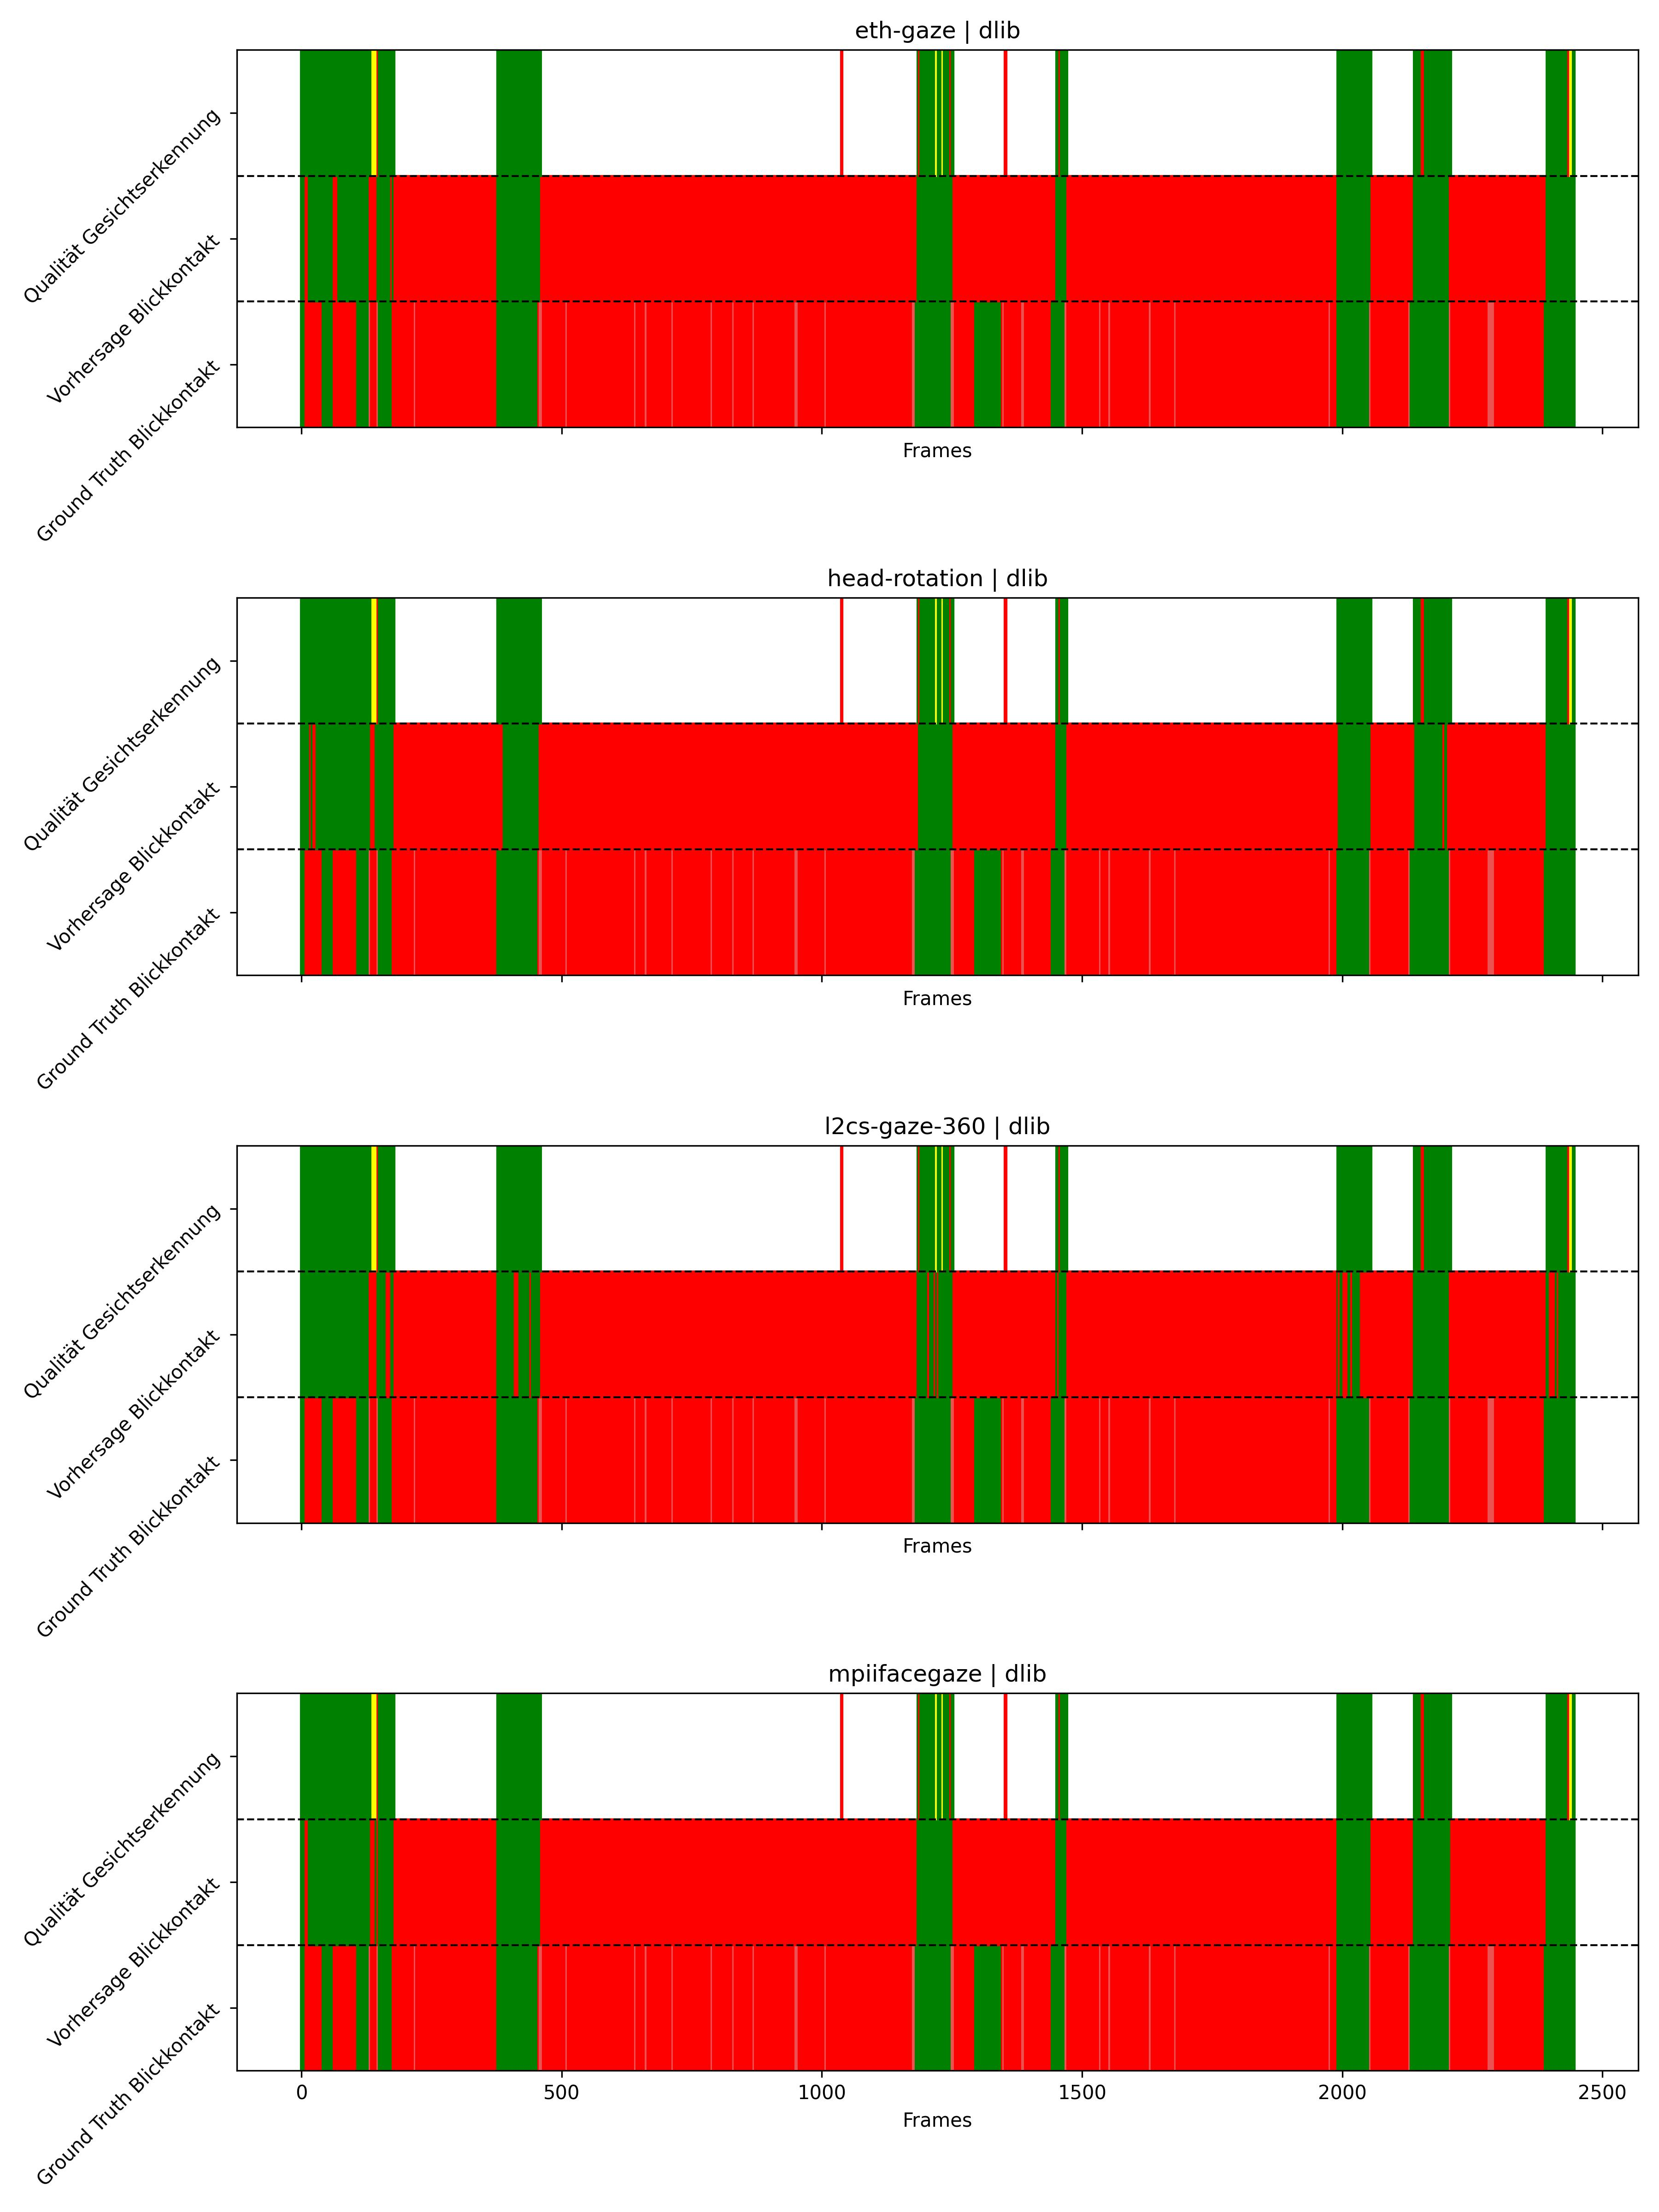
\includegraphics[width=1\linewidth]{appendix/17-dlib-overview-gaze.jpg}
\caption{Überblick über die Ground Truth des Blickkontakts, die Vorhersage des Blickkontakts und die Qualität der Gesichtserkennung mit \dlib. Die Bedeutung der Farben ist in Abbildung \ref{fig:evaluation:gaze:mpiifacegaze} erklärt.  }
\end{figure}

\begin{figure}[H]
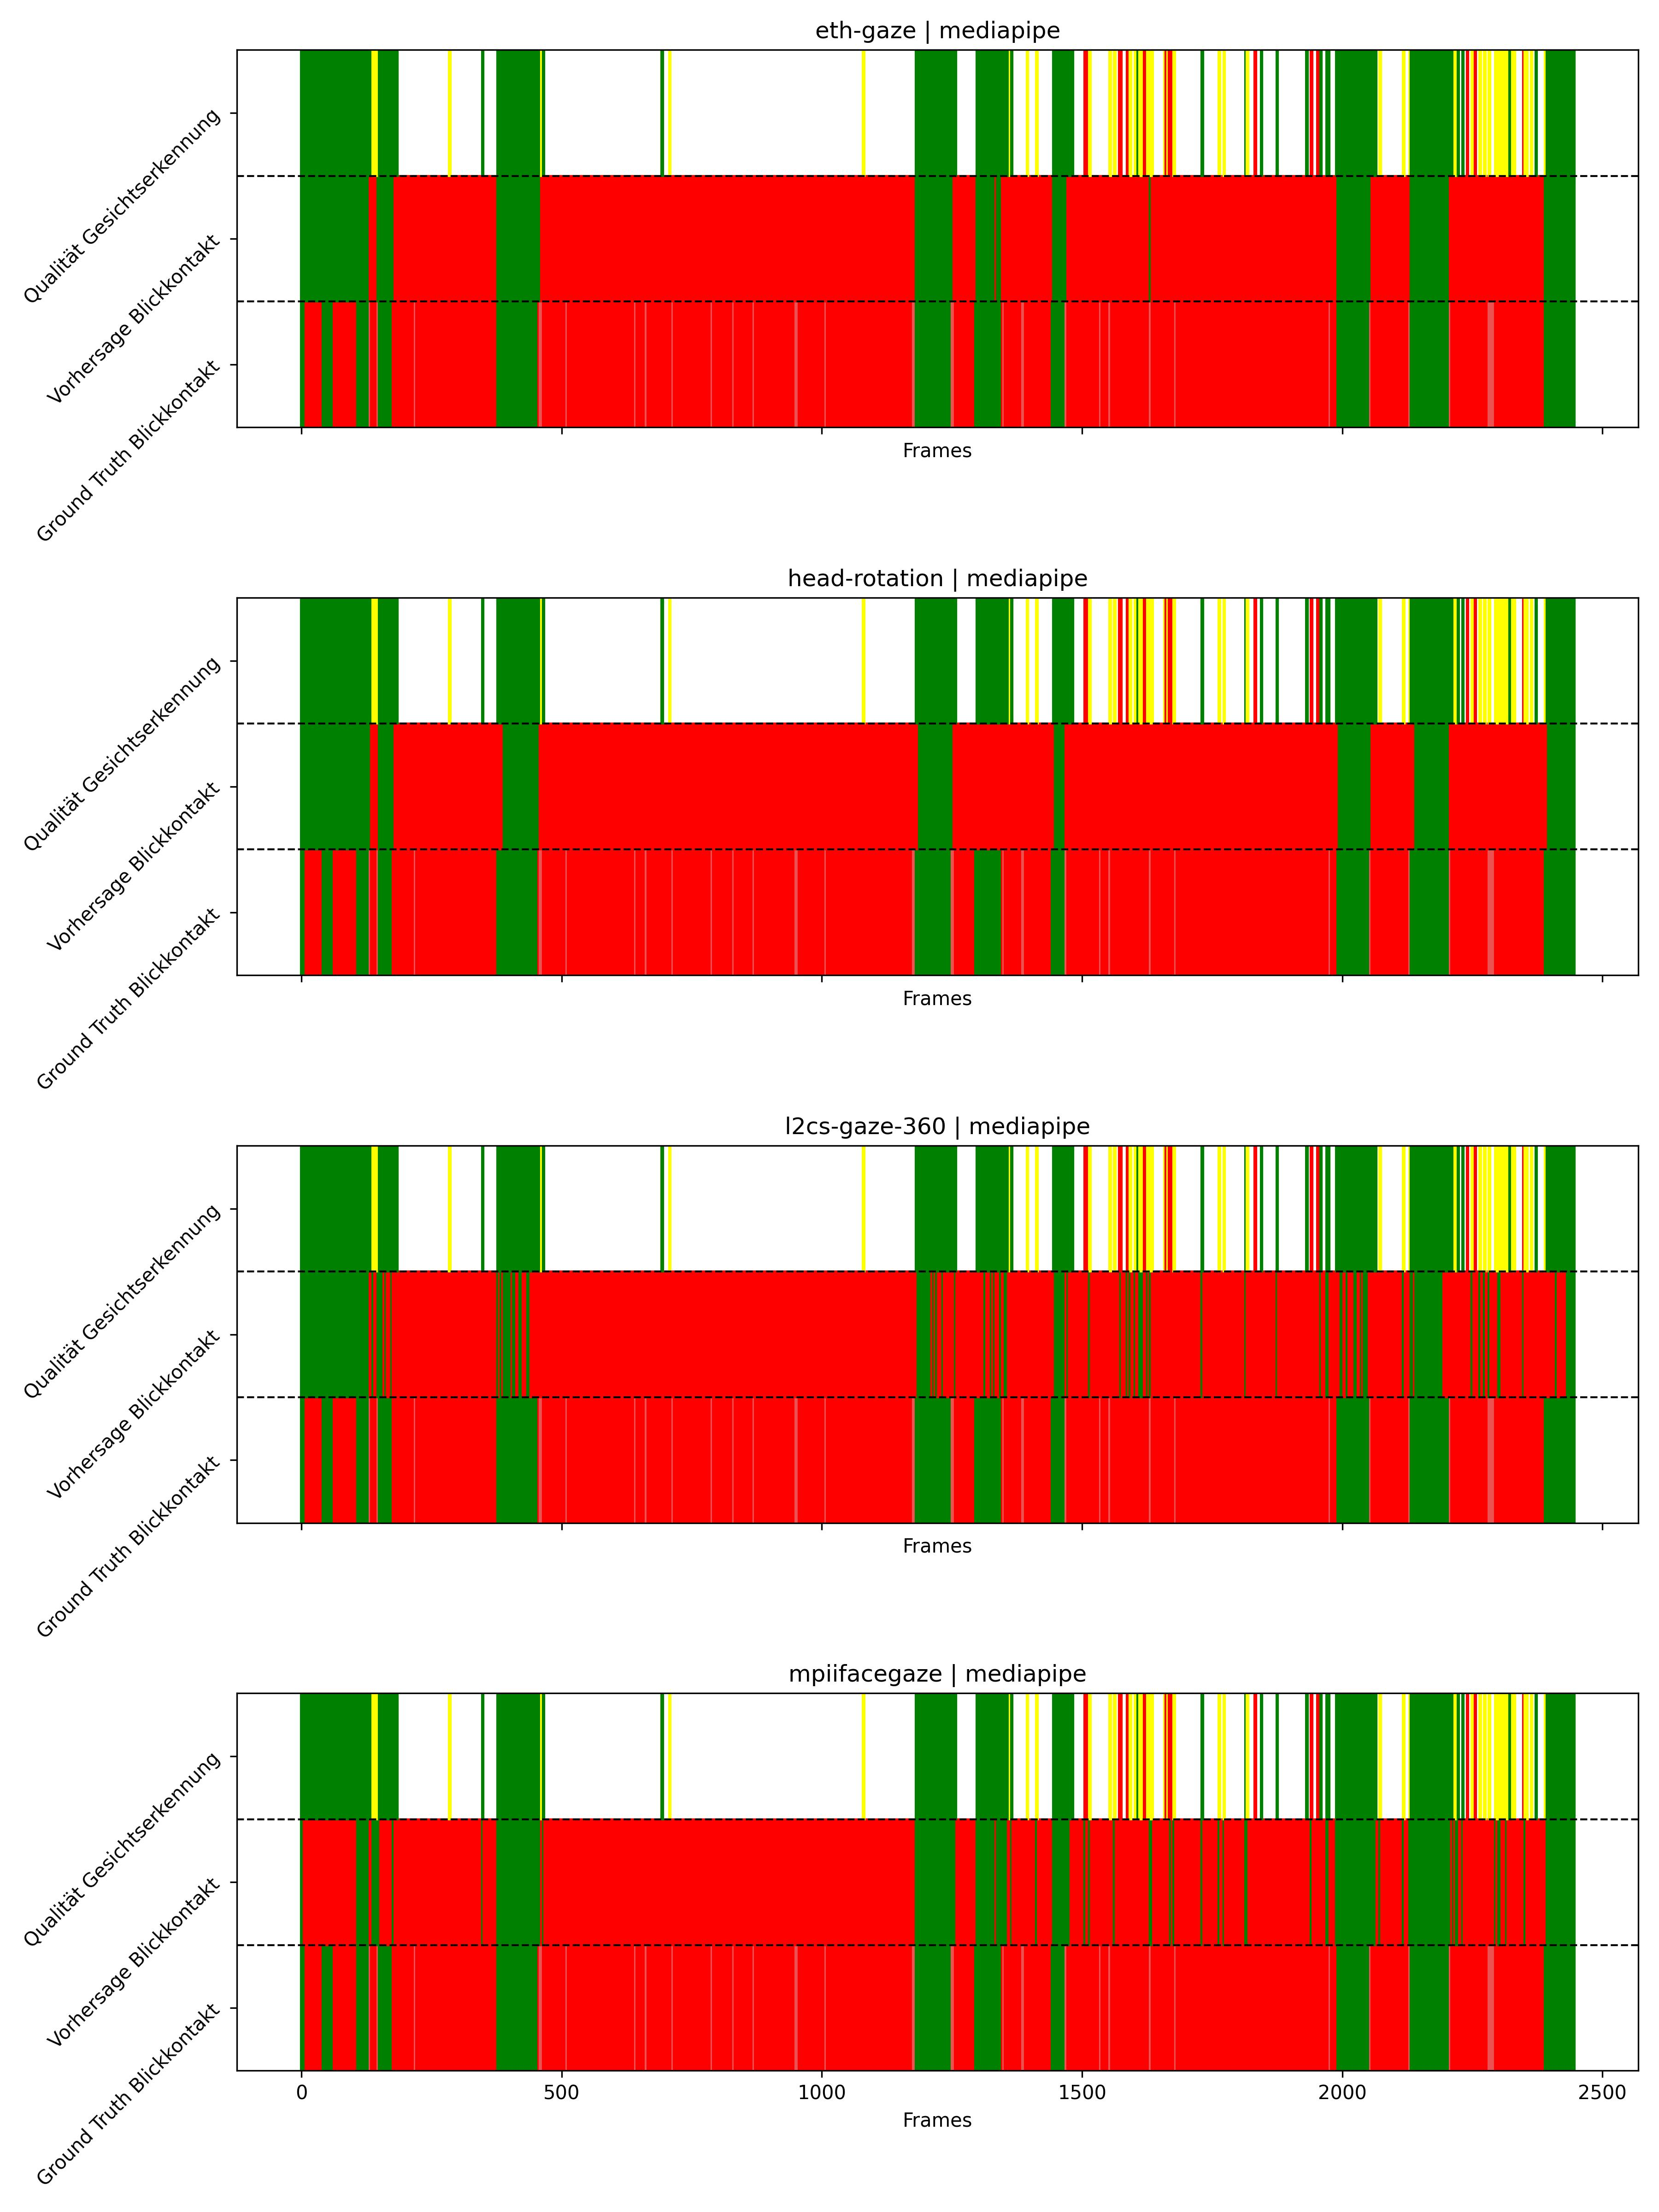
\includegraphics[width=1\linewidth]{appendix/17-mediapipe-overview-gaze.jpg}
\caption{Überblick über die Ground Truth des Blickkontakts, die Vorhersage des Blickkontakts und die Qualität der Gesichtserkennung mit \mediapipe. Die Bedeutung der Farben ist in Abbildung \ref{fig:evaluation:gaze:mpiifacegaze} erklärt.}
\end{figure}

\section{Video 18}
\begin{figure}[H]
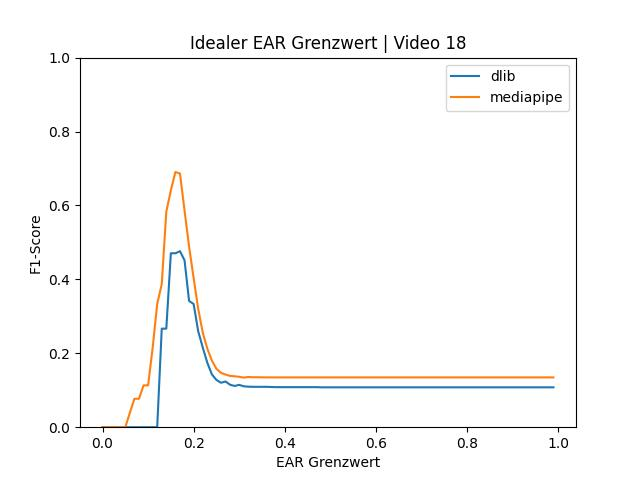
\includegraphics[width=0.7\linewidth]{appendix/18_f1-score-blink.jpg}
\caption{Ergebnisse der Bestimmung des idealen EAR-Grenzwerts für Video 18.}
\end{figure}

\begin{figure}[H]
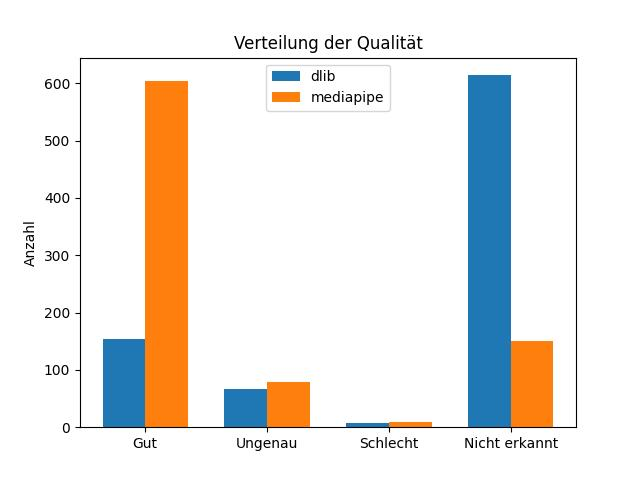
\includegraphics[width=0.7\linewidth]{appendix/18_bar-quality.jpg}
\caption{Aufteilung der Gesichtserkennungsqualität von Video 18.}
\end{figure}

\begin{table}[H]
\centering
\begin{tabular}{l|l|c c |c}
\toprule
\textbf{Gesichtserkennung} & \textbf{Blickrichtung} & \textbf{Seitenlänge} $\hitthresholdsize$ & \textbf{Verschiebung} $\hitthresholdposition$ & \textbf{F1-Score} \\ 
\midrule
\multirow{4}*{dlib}& ETH-XGaze & 0,143 & 0,01 & 0,936  \\ 
& Gaze360 & 0,48 & 0,059 & 0,895 \\ 
& MPIIFaceGaze & 0,071 & 0,022 & 0,615  \\ 
& Kopfrotation & 0,143 & 0,231 & 0,726  \\ 
\hline\multirow{4}*{MediaPipe}& ETH-XGaze & 0,122 & -0,002 & 0,952  \\ 
& Gaze360 & 0,418 & 0,047 & 0,88 \\ 
& MPIIFaceGaze & 0,051 & -0,002 & 0,354  \\ 
& Kopfrotation & 0,133 & 0,231 & 0,921  \\ 
\bottomrule\end{tabular}
\caption{Ergebnis des Hyperparameter-Tunings für die Zone speziell für Video 18.}
\label{tab:appendix:18:local}
\end{table}
\begin{table}[H]
\centering
\begin{tabular}{l|l|c c c c|c c|c}
\toprule
\textbf{Gesichtserkennung} & \textbf{Blickrichtung} & $TP$ & $TN$& $FP$ & $FN$ & \textbf{Precision} & \textbf{Recall} & \textbf{F1-Score} \\ 
\midrule
\multirow{4}*{dlib}& ETH-XGaze & 89 & 729 & 12 & 7 & 0,881 & 0,927 & 0,904 \\ 
& Gaze360 & 82 & 730 & 11 & 14 & 0,882 & 0,854 & 0,868 \\ 
& MPIIFaceGaze & 81 & 635 & 106 & 15 & 0,433 & 0,844 & 0,572 \\ 
& Kopfrotation & 72 & 692 & 49 & 24 & 0,595 & 0,75 & 0,664 \\ 
\hline\multirow{4}*{MediaPipe}& ETH-XGaze & 93 & 733 & 13 & 3 & 0,877 & 0,969 & 0,921 \\ 
& Gaze360 & 79 & 740 & 6 & 17 & 0,929 & 0,823 & 0,873 \\ 
& MPIIFaceGaze & 84 & 340 & 406 & 12 & 0,171 & 0,875 & 0,287 \\ 
& Kopfrotation & 81 & 737 & 9 & 15 & 0,9 & 0,844 & 0,871 \\ 
\bottomrule\end{tabular}
\caption{Zusammensetzung des F1-Scores unter Verwendung der in Kapitel \ref{sec:evaluation:results:gaze:threshold} bestimmten globalen Parameter $\hitthresholdsize$ und $\hitthresholdposition$.}
\label{tab:appendix:18:f1}
\end{table}
\begin{figure}[H]
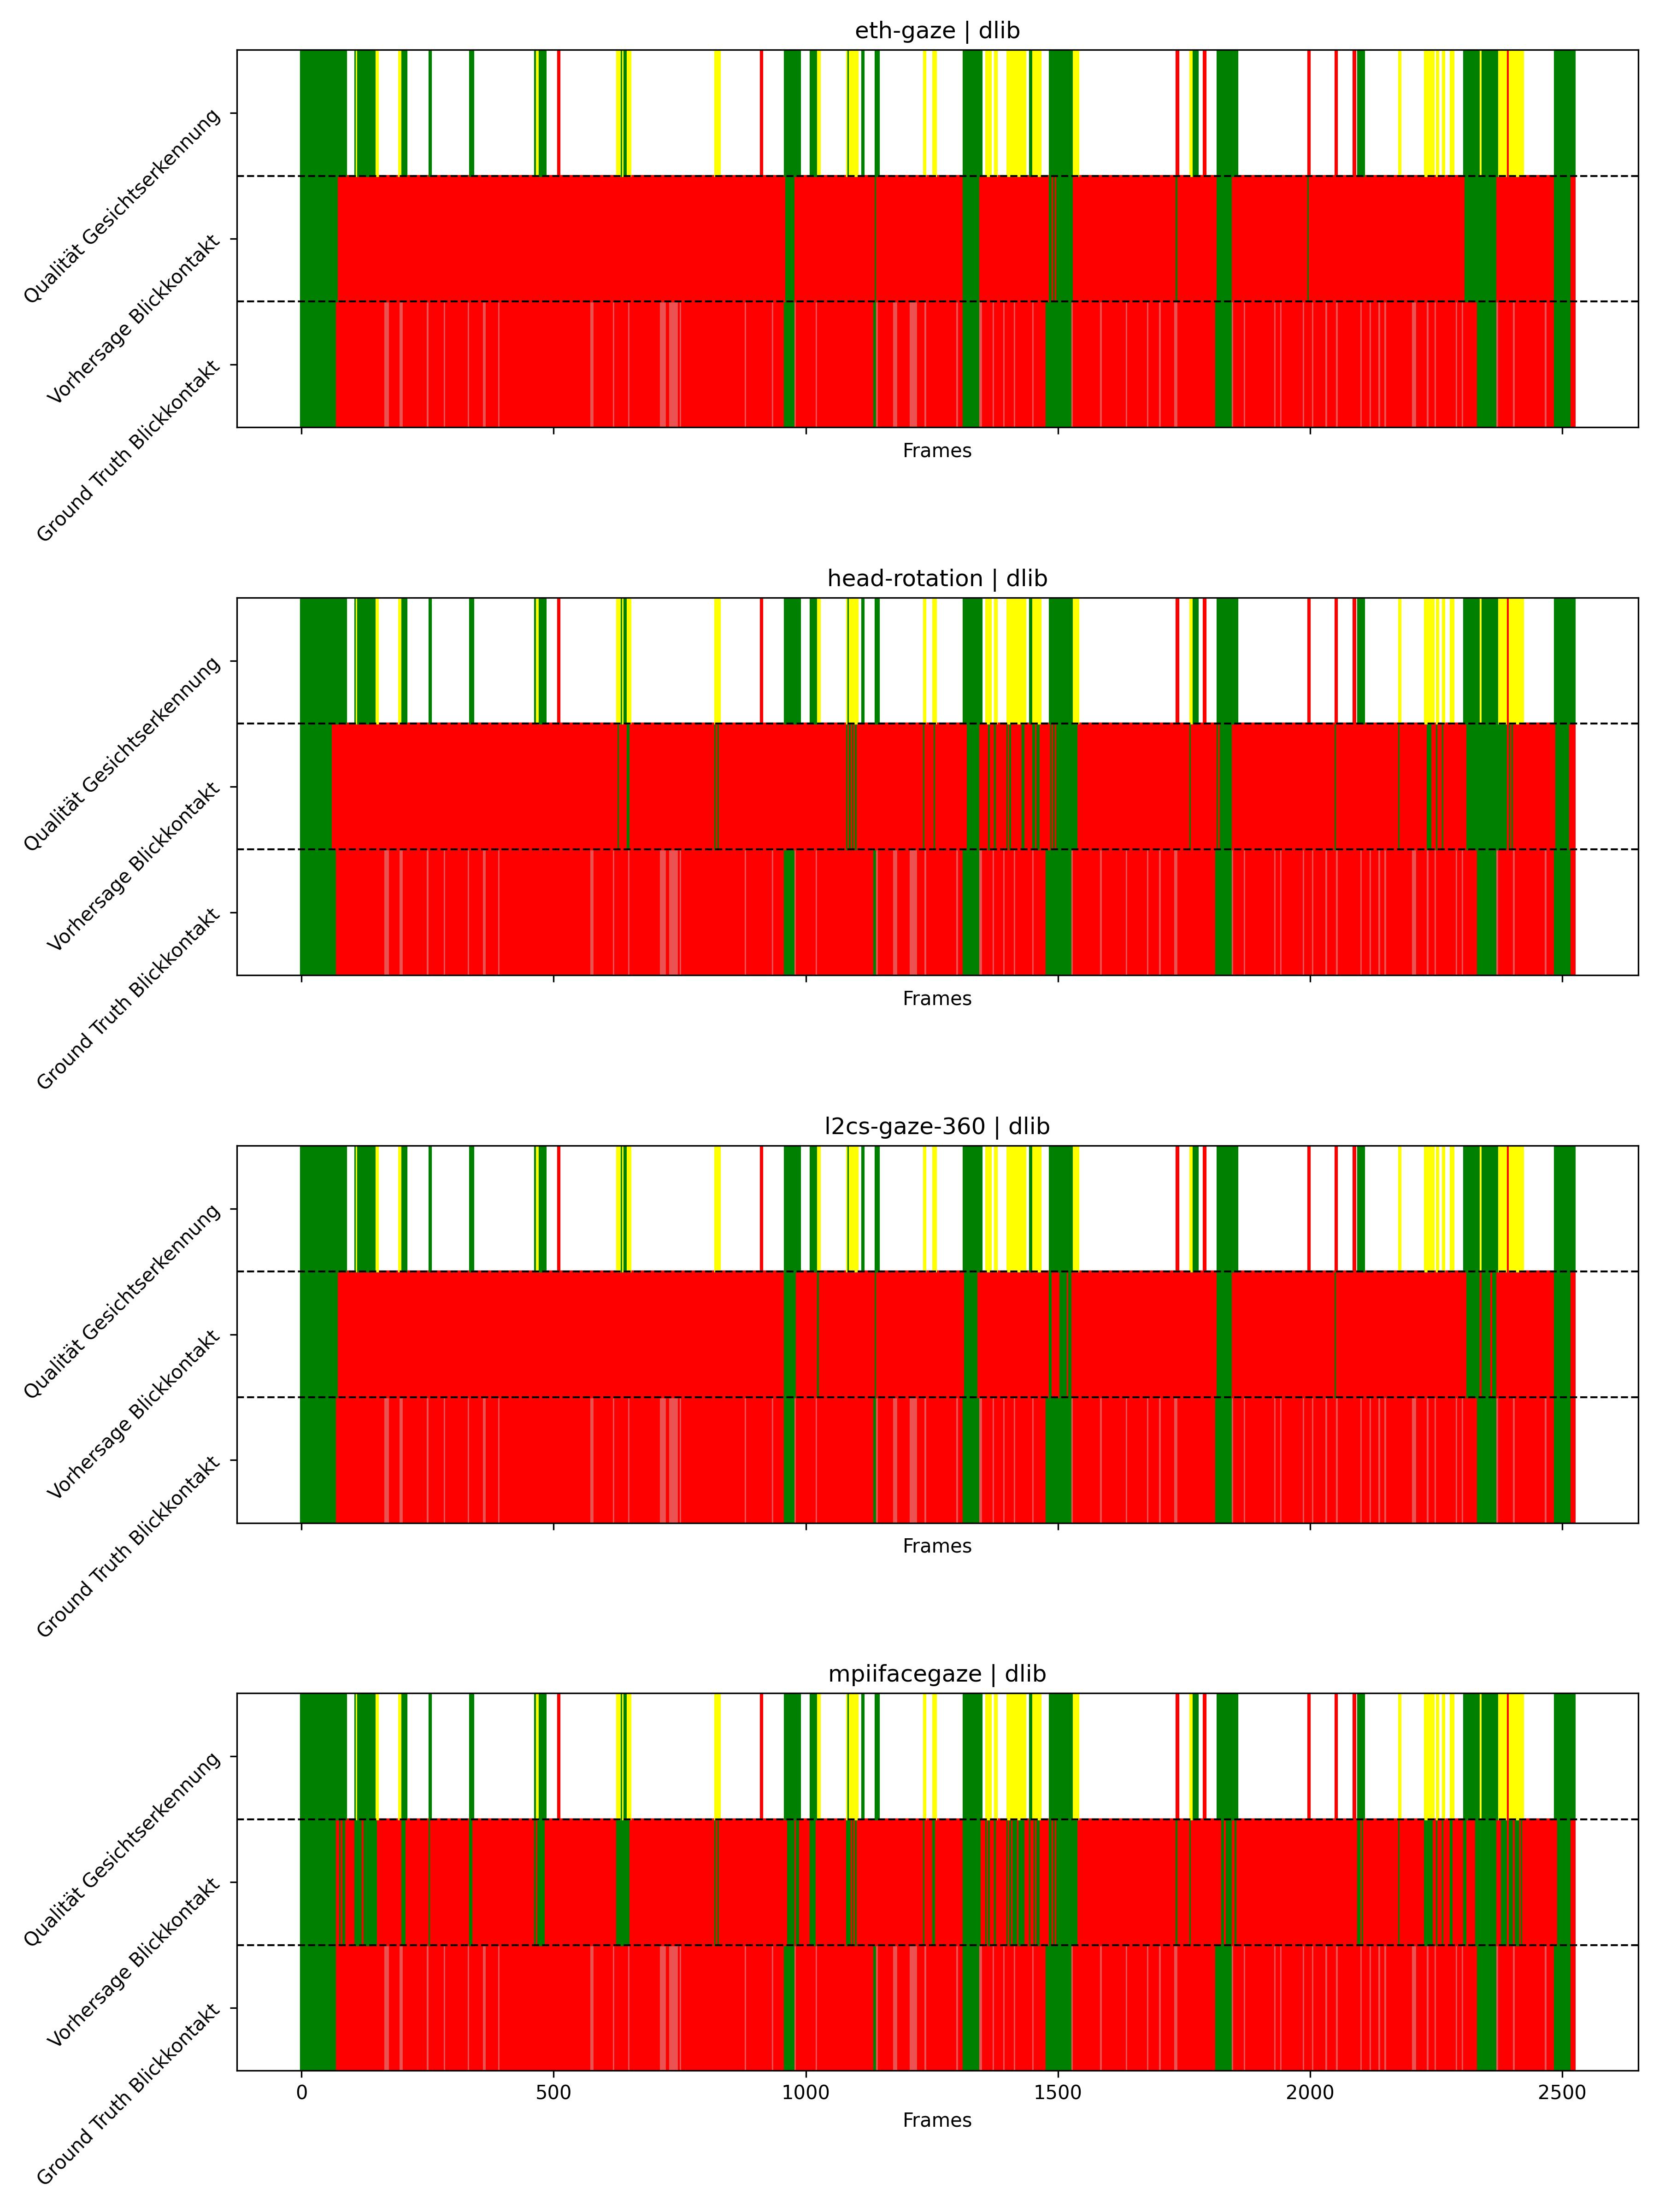
\includegraphics[width=1\linewidth]{appendix/18-dlib-overview-gaze.jpg}
\caption{Überblick über die Ground Truth des Blickkontakts, die Vorhersage des Blickkontakts und die Qualität der Gesichtserkennung mit \dlib. Die Bedeutung der Farben ist in Abbildung \ref{fig:evaluation:gaze:mpiifacegaze} erklärt.  }
\end{figure}

\begin{figure}[H]
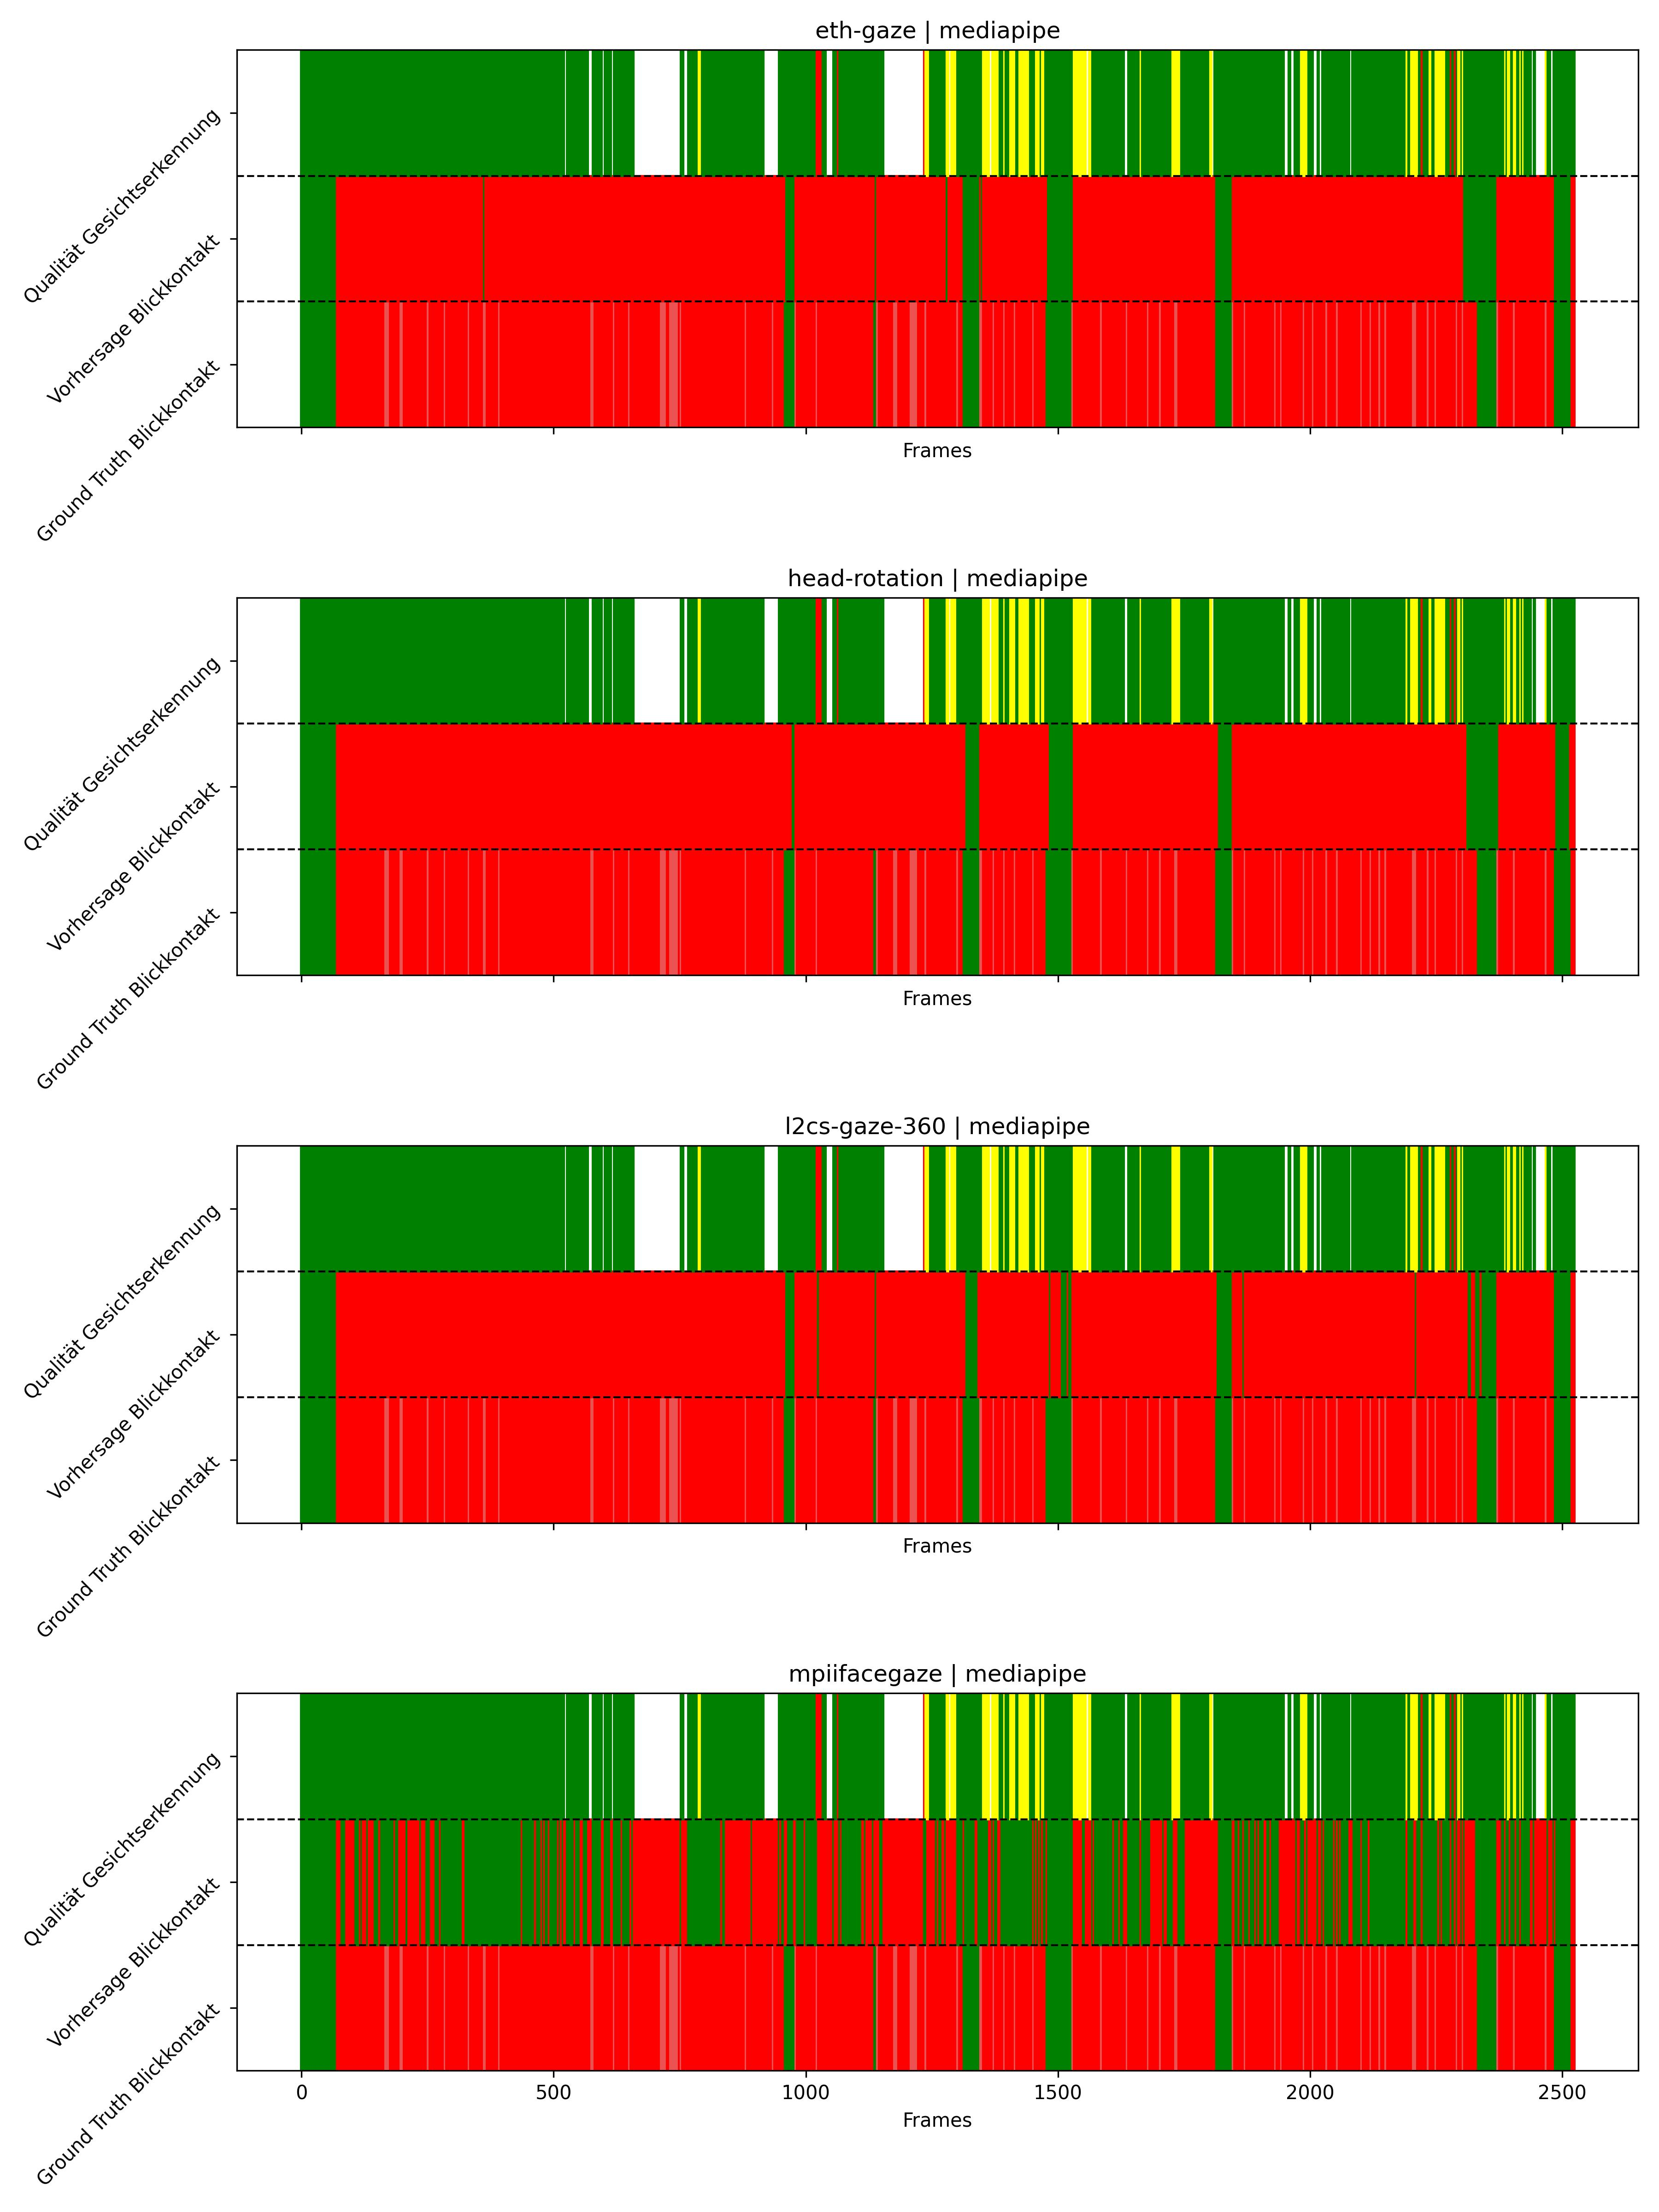
\includegraphics[width=1\linewidth]{appendix/18-mediapipe-overview-gaze.jpg}
\caption{Überblick über die Ground Truth des Blickkontakts, die Vorhersage des Blickkontakts und die Qualität der Gesichtserkennung mit \mediapipe. Die Bedeutung der Farben ist in Abbildung \ref{fig:evaluation:gaze:mpiifacegaze} erklärt.}
\end{figure}

\section{Video 19}
\begin{figure}[H]
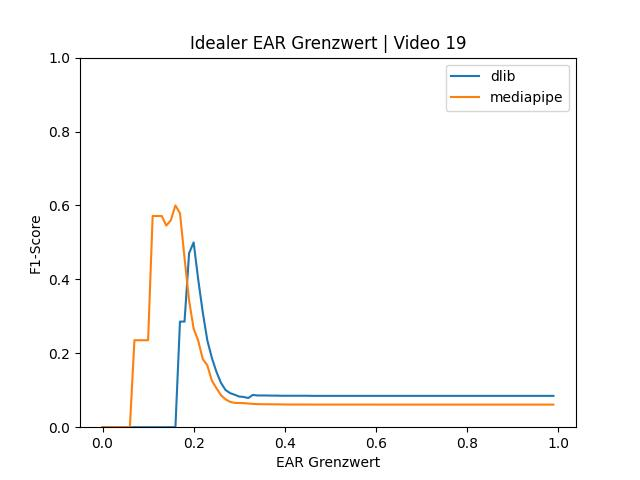
\includegraphics[width=0.7\linewidth]{appendix/19_f1-score-blink.jpg}
\caption{Ergebnisse der Bestimmung des idealen EAR-Grenzwerts für Video 19.}
\end{figure}

\begin{figure}[H]
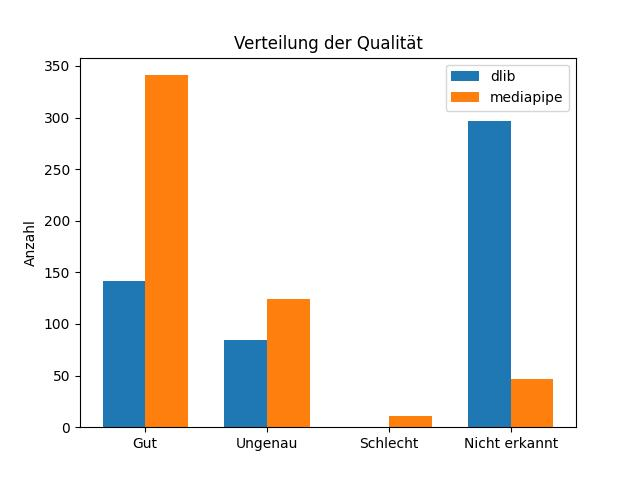
\includegraphics[width=0.7\linewidth]{appendix/19_bar-quality.jpg}
\caption{Aufteilung der Gesichtserkennungsqualität von Video 19.}
\end{figure}

\begin{table}[H]
\centering
\begin{tabular}{l|l|c c |c}
\toprule
\textbf{Gesichtserkennung} & \textbf{Blickrichtung} & \textbf{Seitenlänge} $\hitthresholdsize$ & \textbf{Verschiebung} $\hitthresholdposition$ & \textbf{F1-Score} \\ 
\midrule
\multirow{4}*{dlib}& ETH-XGaze & 0,153 & -0,002 & 0,972  \\ 
& Gaze360 & 0,398 & 0,01 & 0,961 \\ 
& MPIIFaceGaze & 0,112 & 0,059 & 0,678  \\ 
& Kopfrotation & 0,163 & 0,194 & 0,74  \\ 
\hline\multirow{4}*{MediaPipe}& ETH-XGaze & 0,143 & -0,002 & 0,971  \\ 
& Gaze360 & 0,398 & 0,022 & 0,956 \\ 
& MPIIFaceGaze & 0,031 & -0,027 & 0,56  \\ 
& Kopfrotation & 0,122 & 0,194 & 0,87  \\ 
\bottomrule\end{tabular}
\caption{Ergebnis des Hyperparameter-Tunings für die Zone speziell für Video 19.}
\label{tab:appendix:19:local}
\end{table}
\begin{table}[H]
\centering
\begin{tabular}{l|l|c c c c|c c|c}
\toprule
\textbf{Gesichtserkennung} & \textbf{Blickrichtung} & $TP$ & $TN$& $FP$ & $FN$ & \textbf{Precision} & \textbf{Recall} & \textbf{F1-Score} \\ 
\midrule
\multirow{4}*{dlib}& ETH-XGaze & 87 & 428 & 7 & 1 & 0,926 & 0,989 & 0,956 \\ 
& Gaze360 & 87 & 424 & 11 & 1 & 0,888 & 0,989 & 0,935 \\ 
& MPIIFaceGaze & 79 & 316 & 119 & 9 & 0,399 & 0,898 & 0,552 \\ 
& Kopfrotation & 81 & 384 & 51 & 7 & 0,614 & 0,92 & 0,736 \\ 
\hline\multirow{4}*{MediaPipe}& ETH-XGaze & 87 & 426 & 9 & 1 & 0,906 & 0,989 & 0,946 \\ 
& Gaze360 & 87 & 424 & 11 & 1 & 0,888 & 0,989 & 0,935 \\ 
& MPIIFaceGaze & 81 & 223 & 212 & 7 & 0,276 & 0,92 & 0,425 \\ 
& Kopfrotation & 84 & 408 & 27 & 4 & 0,757 & 0,955 & 0,844 \\ 
\bottomrule\end{tabular}
\caption{Zusammensetzung des F1-Scores unter Verwendung der in Kapitel \ref{sec:evaluation:results:gaze:threshold} bestimmten globalen Parameter $\hitthresholdsize$ und $\hitthresholdposition$.}
\label{tab:appendix:19:f1}
\end{table}
\begin{figure}[H]
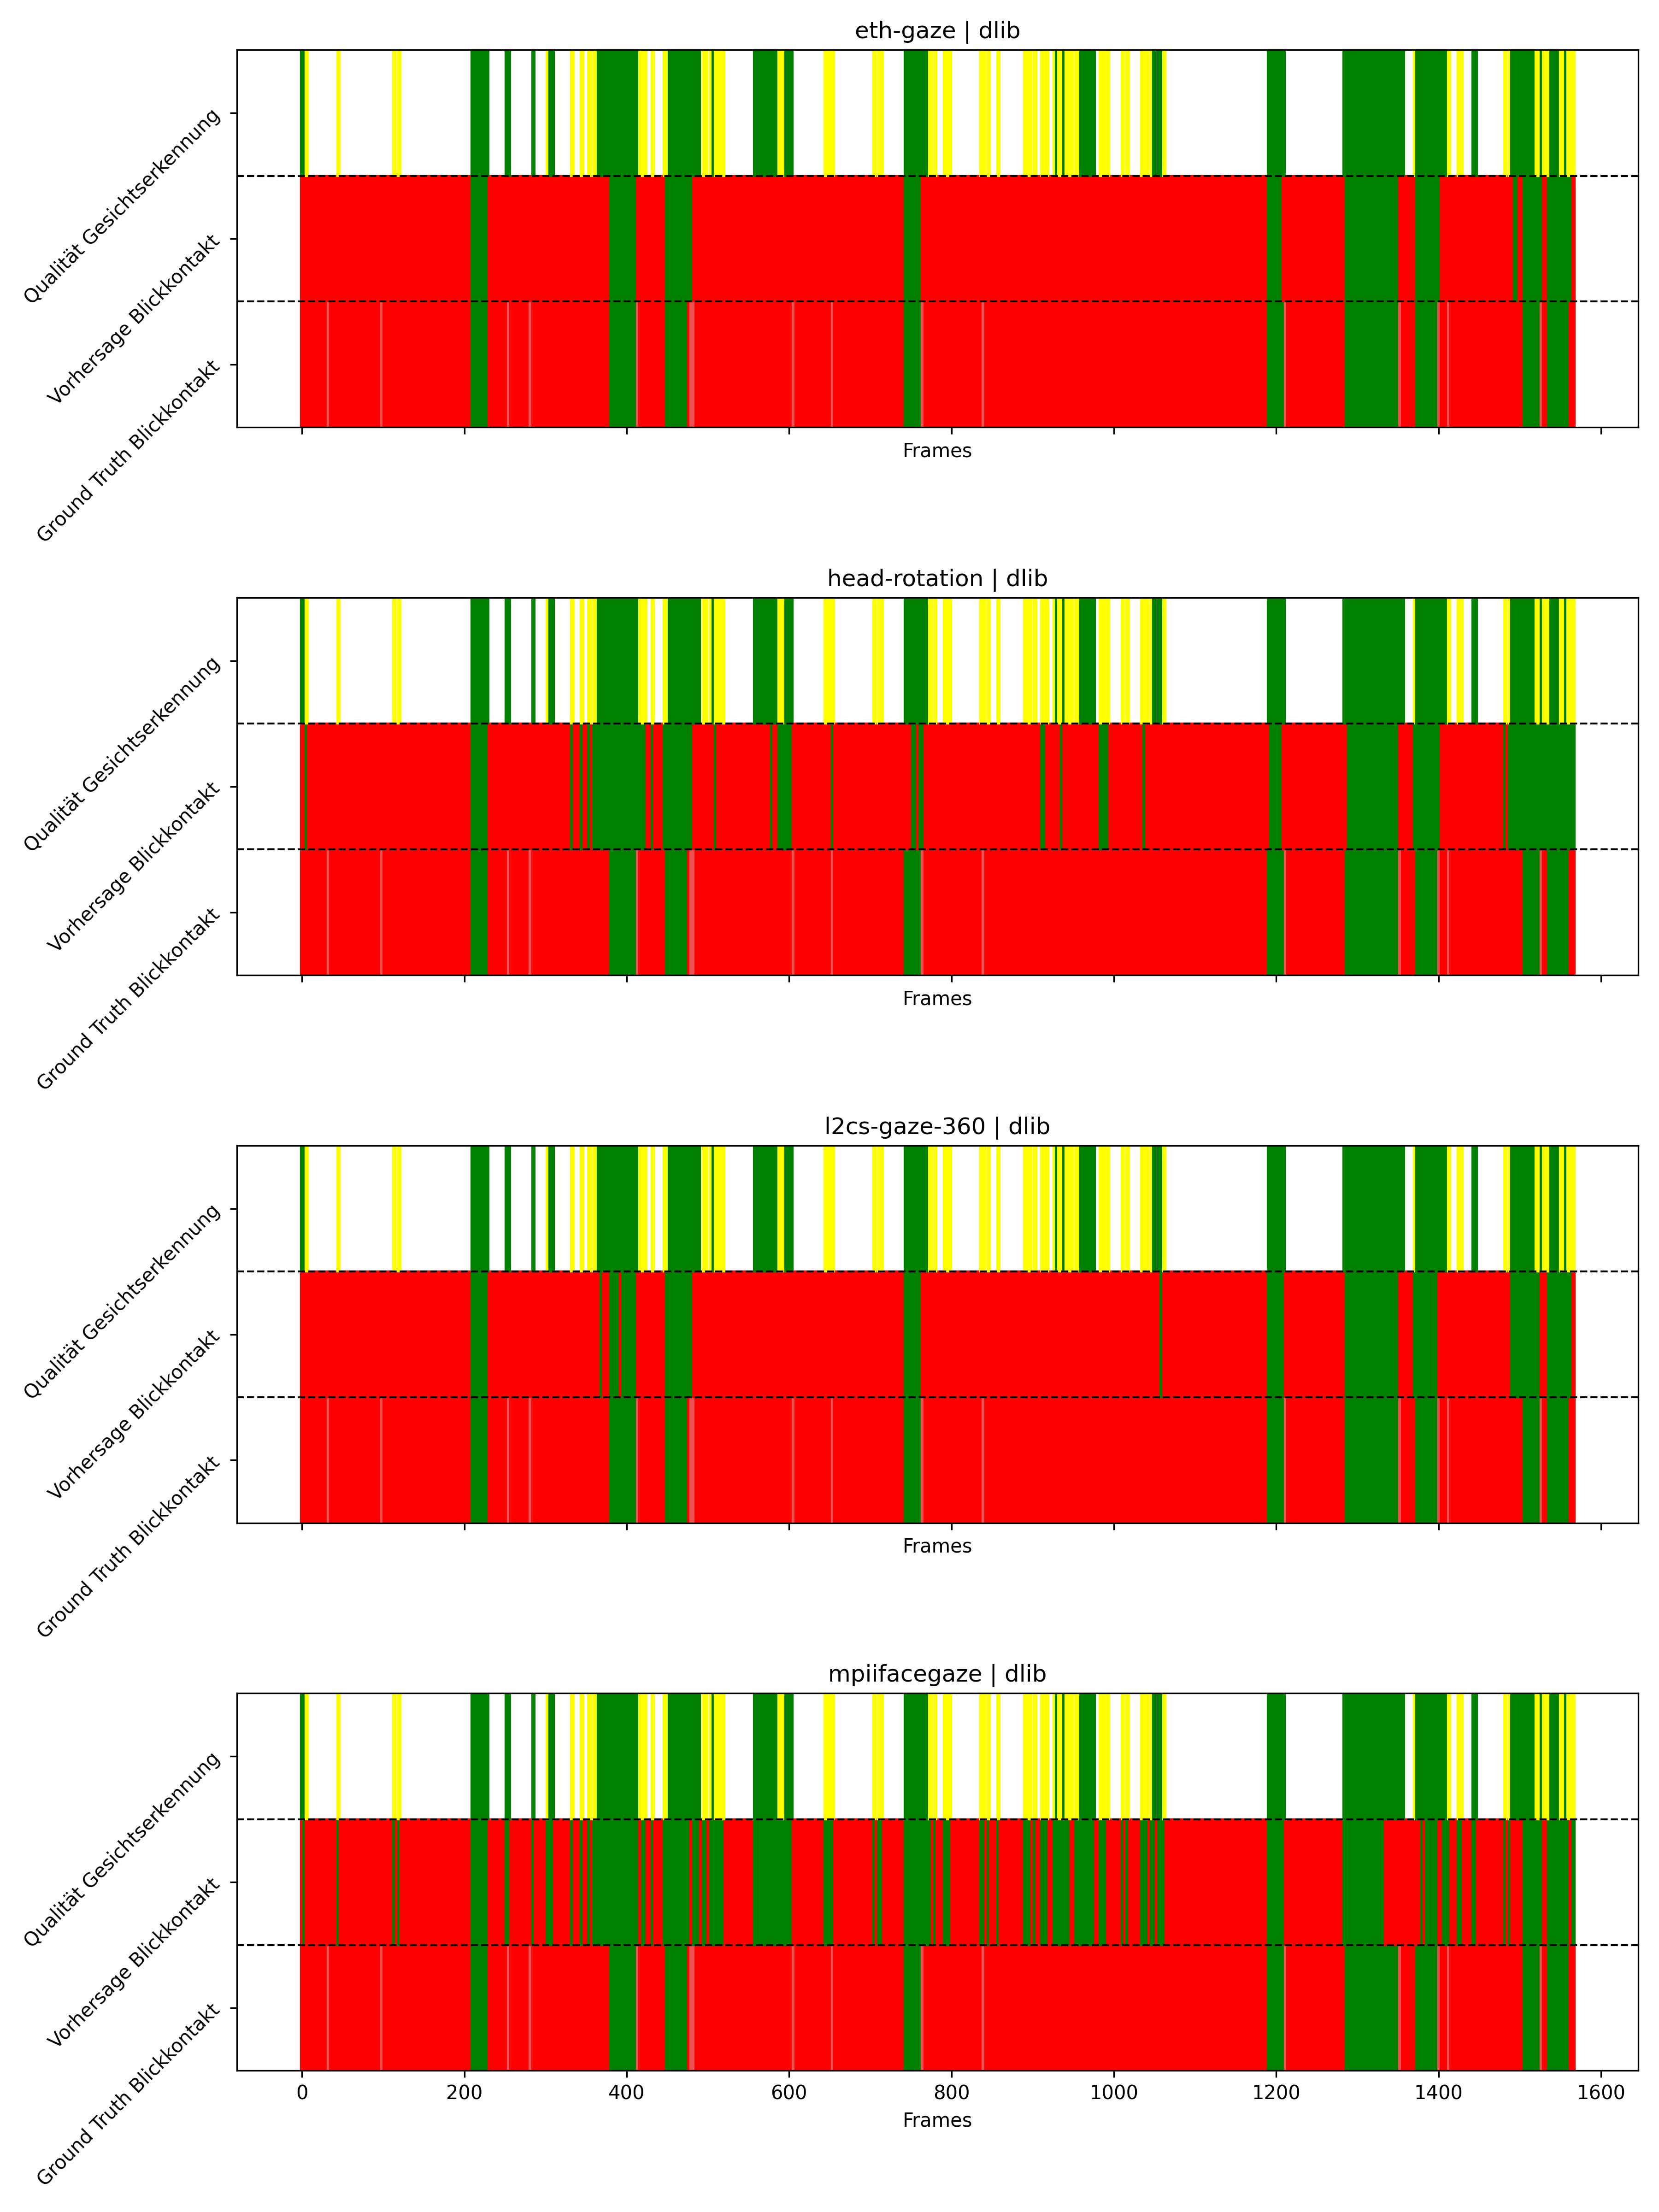
\includegraphics[width=1\linewidth]{appendix/19-dlib-overview-gaze.jpg}
\caption{Überblick über die Ground Truth des Blickkontakts, die Vorhersage des Blickkontakts und die Qualität der Gesichtserkennung mit \dlib. Die Bedeutung der Farben ist in Abbildung \ref{fig:evaluation:gaze:mpiifacegaze} erklärt.  }
\end{figure}

\begin{figure}[H]
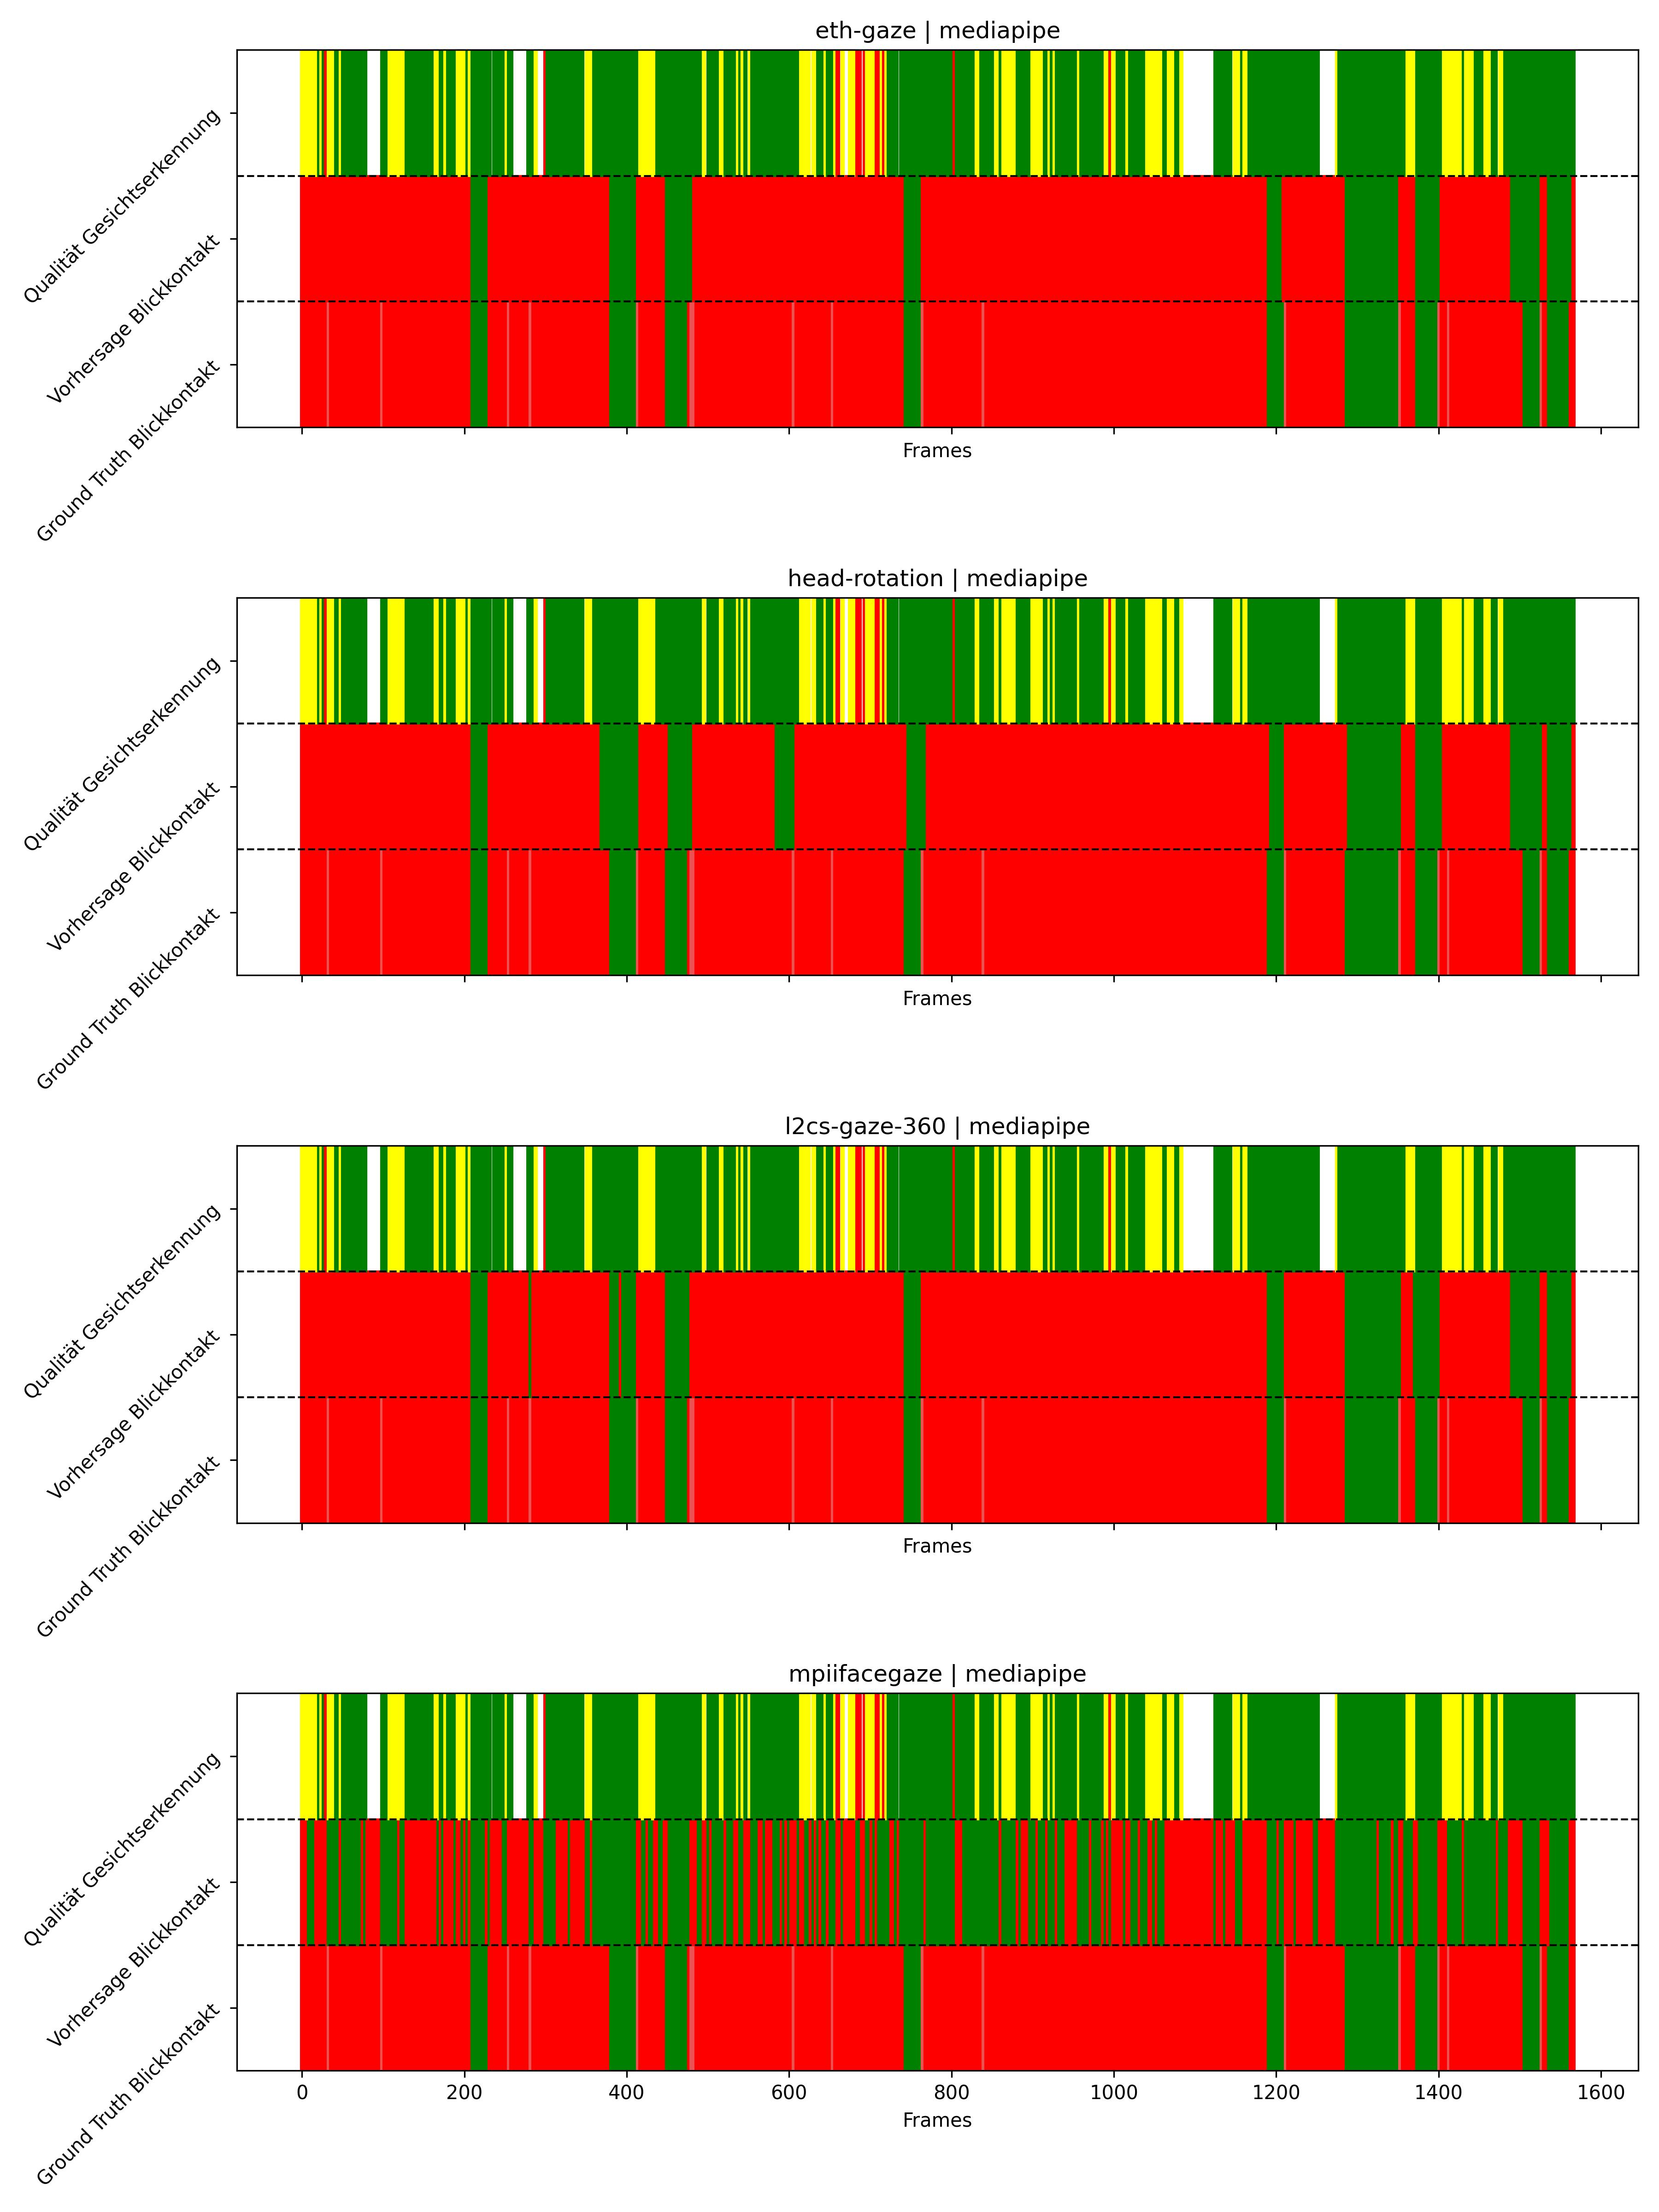
\includegraphics[width=1\linewidth]{appendix/19-mediapipe-overview-gaze.jpg}
\caption{Überblick über die Ground Truth des Blickkontakts, die Vorhersage des Blickkontakts und die Qualität der Gesichtserkennung mit \mediapipe. Die Bedeutung der Farben ist in Abbildung \ref{fig:evaluation:gaze:mpiifacegaze} erklärt.}
\end{figure}

\section{Video 20}
\begin{figure}[H]
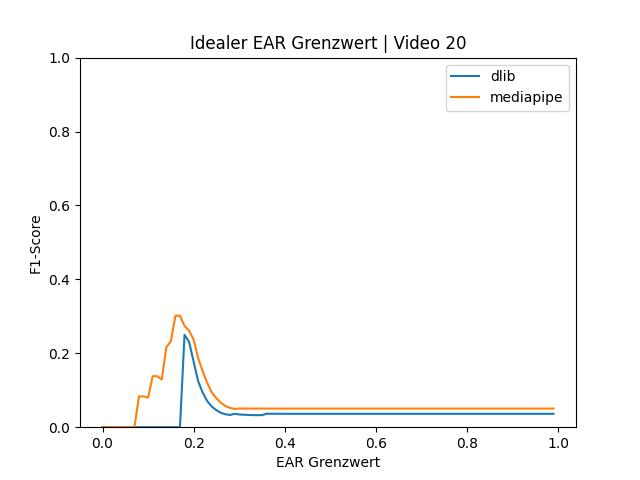
\includegraphics[width=0.7\linewidth]{appendix/20_f1-score-blink.jpg}
\caption{Ergebnisse der Bestimmung des idealen EAR-Grenzwerts für Video 20.}
\end{figure}

\begin{figure}[H]
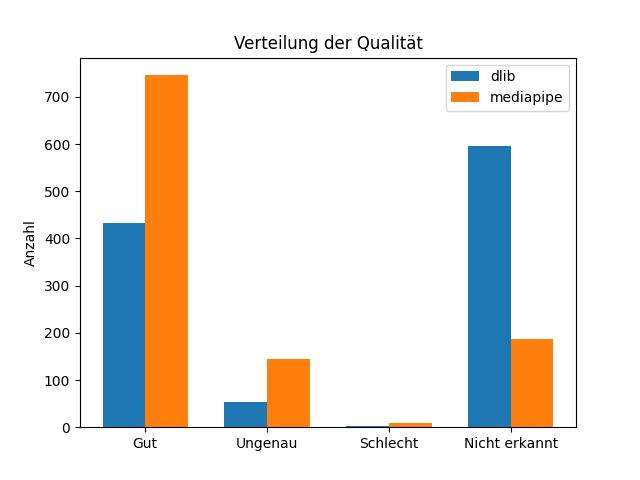
\includegraphics[width=0.7\linewidth]{appendix/20_bar-quality.jpg}
\caption{Aufteilung der Gesichtserkennungsqualität von Video 20.}
\end{figure}

\begin{table}[H]
\centering
\begin{tabular}{l|l|c c |c}
\toprule
\textbf{Gesichtserkennung} & \textbf{Blickrichtung} & \textbf{Seitenlänge} $\hitthresholdsize$ & \textbf{Verschiebung} $\hitthresholdposition$ & \textbf{F1-Score} \\ 
\midrule
\multirow{4}*{dlib}& ETH-XGaze & 0,173 & -0,002 & 0,945  \\ 
& Gaze360 & 0,49 & 0,035 & 0,895 \\ 
& MPIIFaceGaze & 0,051 & -0,027 & 0,795  \\ 
& Kopfrotation & 0,173 & 0,218 & 0,78  \\ 
\hline\multirow{4}*{MediaPipe}& ETH-XGaze & 0,173 & -0,014 & 0,961  \\ 
& Gaze360 & 0,296 & 0,035 & 0,895 \\ 
& MPIIFaceGaze & 0,041 & -0,039 & 0,596  \\ 
& Kopfrotation & 0,163 & 0,194 & 0,803  \\ 
\bottomrule\end{tabular}
\caption{Ergebnis des Hyperparameter-Tunings für die Zone speziell für Video 20.}
\label{tab:appendix:20:local}
\end{table}
\begin{table}[H]
\centering
\begin{tabular}{l|l|c c c c|c c|c}
\toprule
\textbf{Gesichtserkennung} & \textbf{Blickrichtung} & $TP$ & $TN$& $FP$ & $FN$ & \textbf{Precision} & \textbf{Recall} & \textbf{F1-Score} \\ 
\midrule
\multirow{4}*{dlib}& ETH-XGaze & 294 & 745 & 20 & 23 & 0,936 & 0,927 & 0,932 \\ 
& Gaze360 & 290 & 716 & 49 & 27 & 0,855 & 0,915 & 0,884 \\ 
& MPIIFaceGaze & 299 & 624 & 141 & 18 & 0,68 & 0,943 & 0,79 \\ 
& Kopfrotation & 264 & 654 & 111 & 53 & 0,704 & 0,833 & 0,763 \\ 
\hline\multirow{4}*{MediaPipe}& ETH-XGaze & 314 & 725 & 41 & 4 & 0,885 & 0,987 & 0,933 \\ 
& Gaze360 & 305 & 696 & 70 & 13 & 0,813 & 0,959 & 0,88 \\ 
& MPIIFaceGaze & 304 & 354 & 412 & 14 & 0,425 & 0,956 & 0,588 \\ 
& Kopfrotation & 291 & 638 & 128 & 27 & 0,695 & 0,915 & 0,79 \\ 
\bottomrule\end{tabular}
\caption{Zusammensetzung des F1-Scores unter Verwendung der in Kapitel \ref{sec:evaluation:results:gaze:threshold} bestimmten globalen Parameter $\hitthresholdsize$ und $\hitthresholdposition$.}
\label{tab:appendix:20:f1}
\end{table}
\begin{figure}[H]
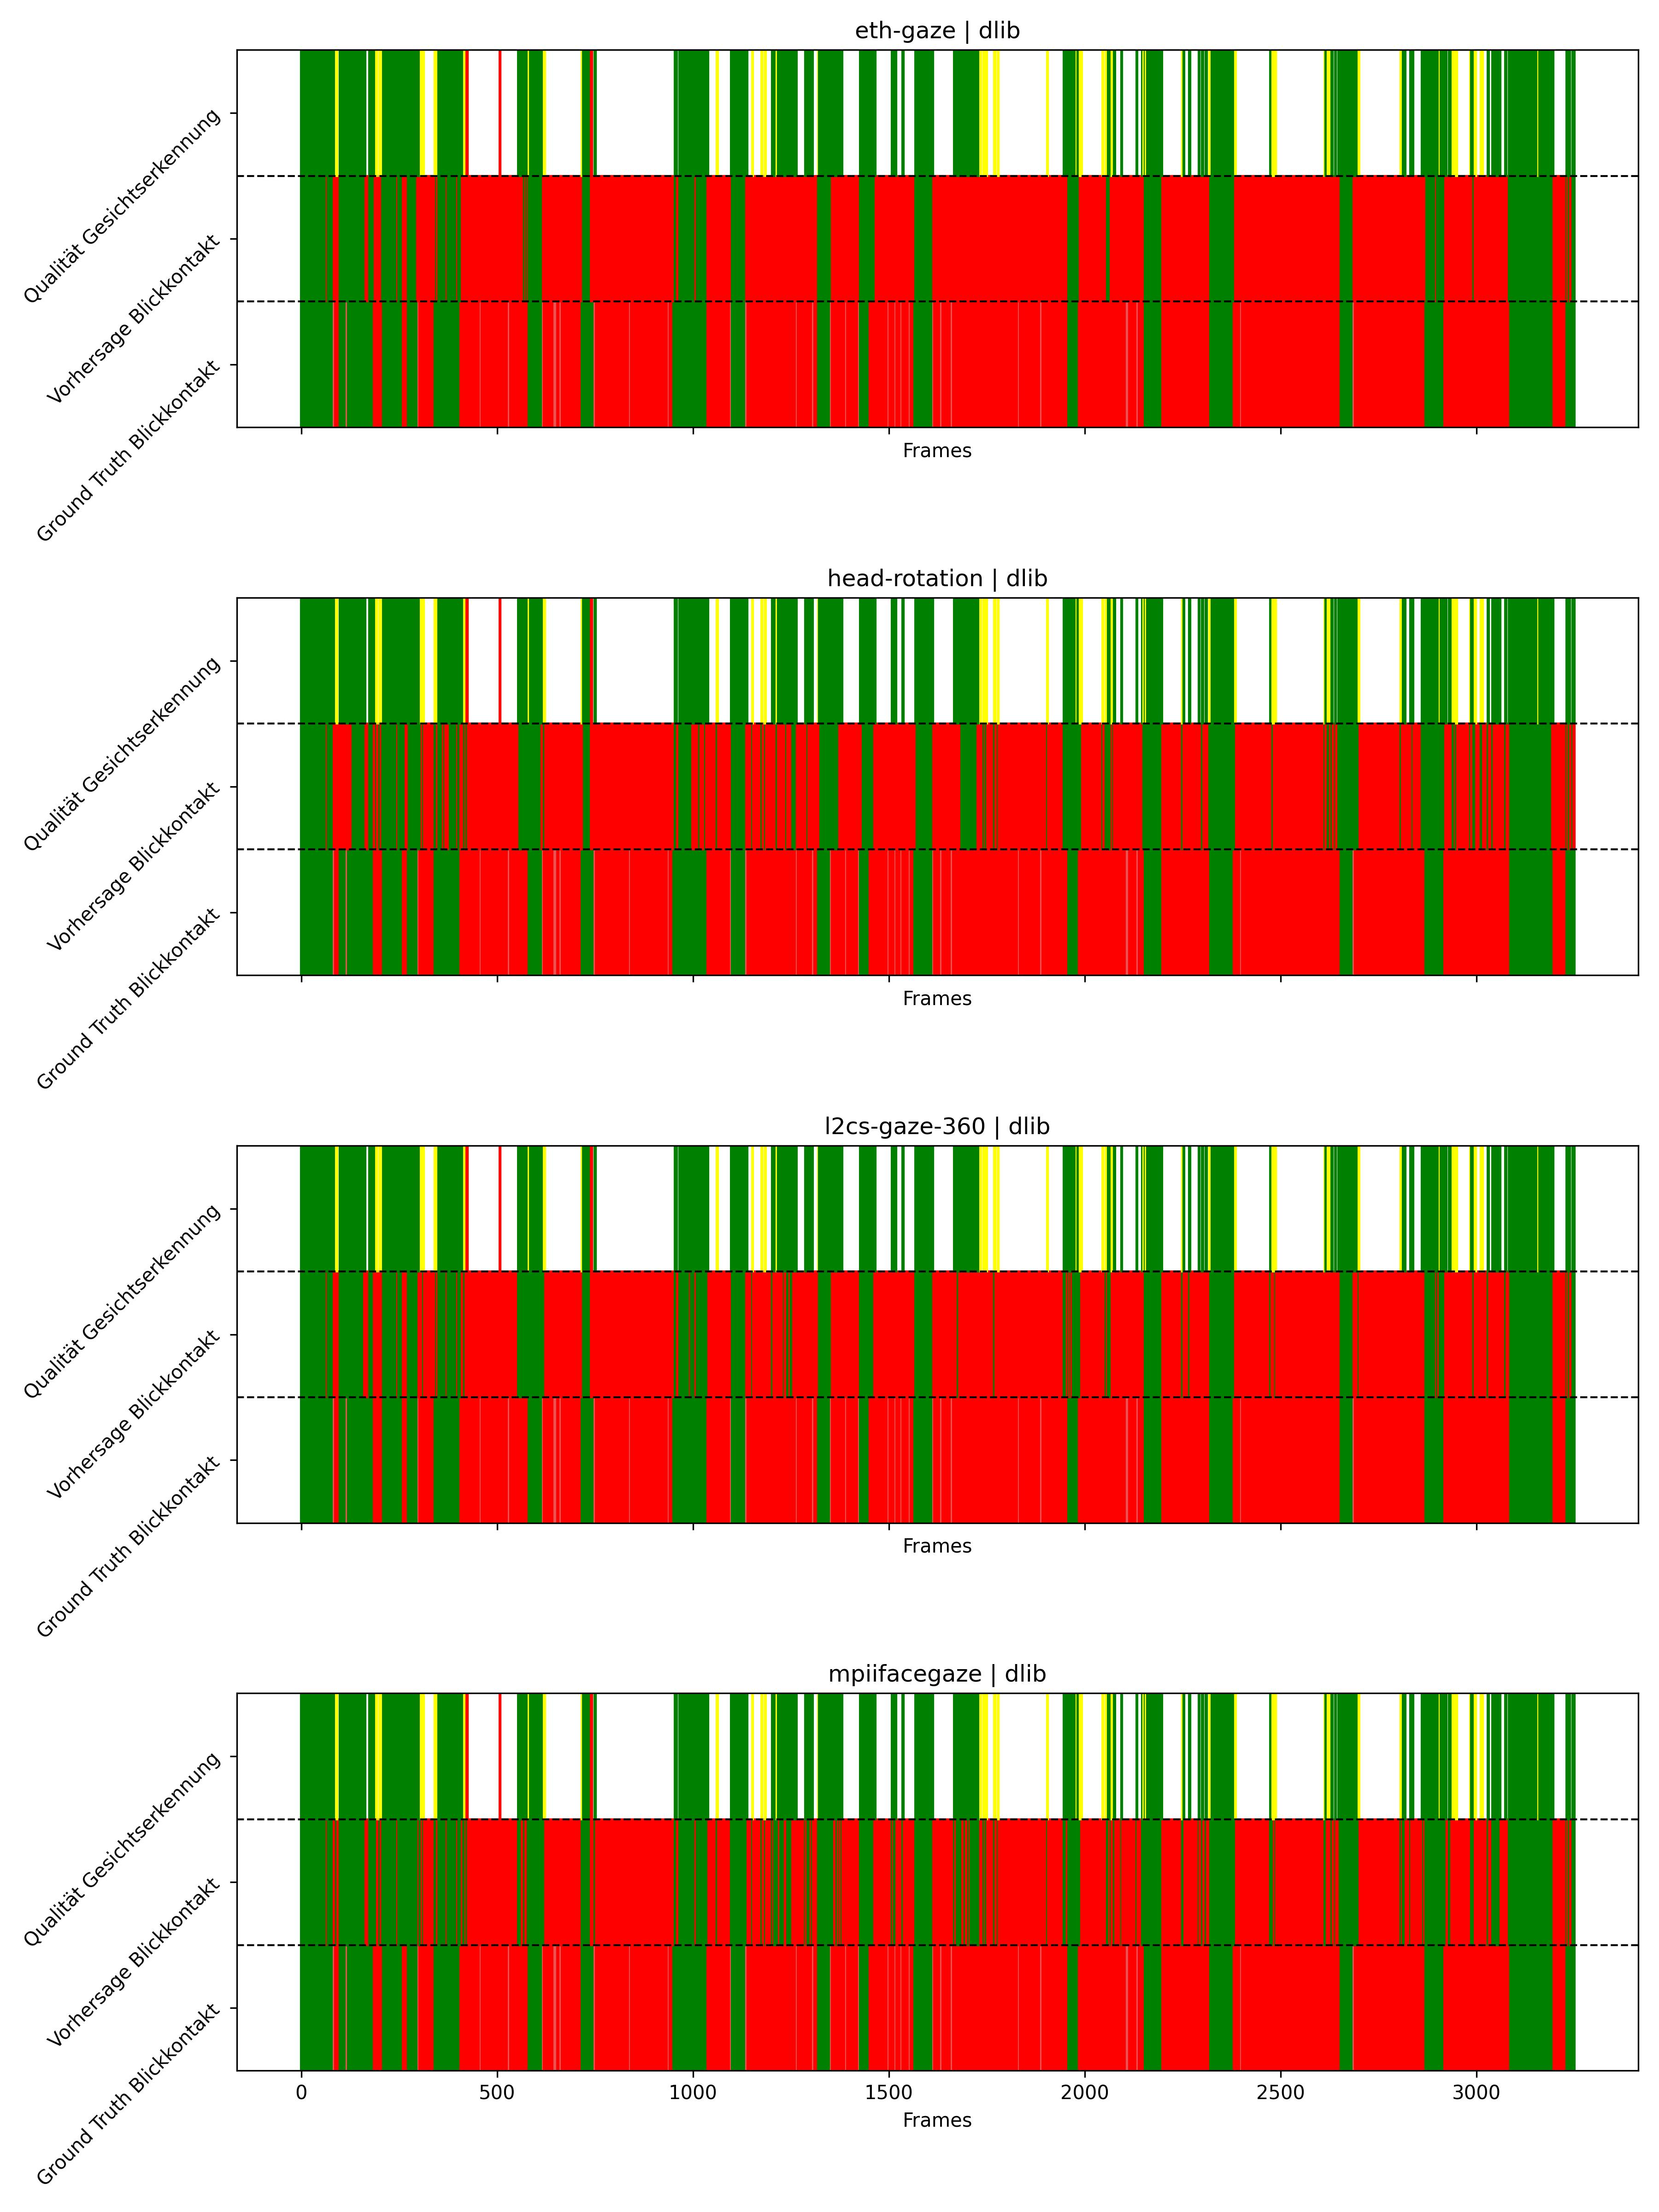
\includegraphics[width=1\linewidth]{appendix/20-dlib-overview-gaze.jpg}
\caption{Überblick über die Ground Truth des Blickkontakts, die Vorhersage des Blickkontakts und die Qualität der Gesichtserkennung mit \dlib. Die Bedeutung der Farben ist in Abbildung \ref{fig:evaluation:gaze:mpiifacegaze} erklärt.  }
\end{figure}

\begin{figure}[H]
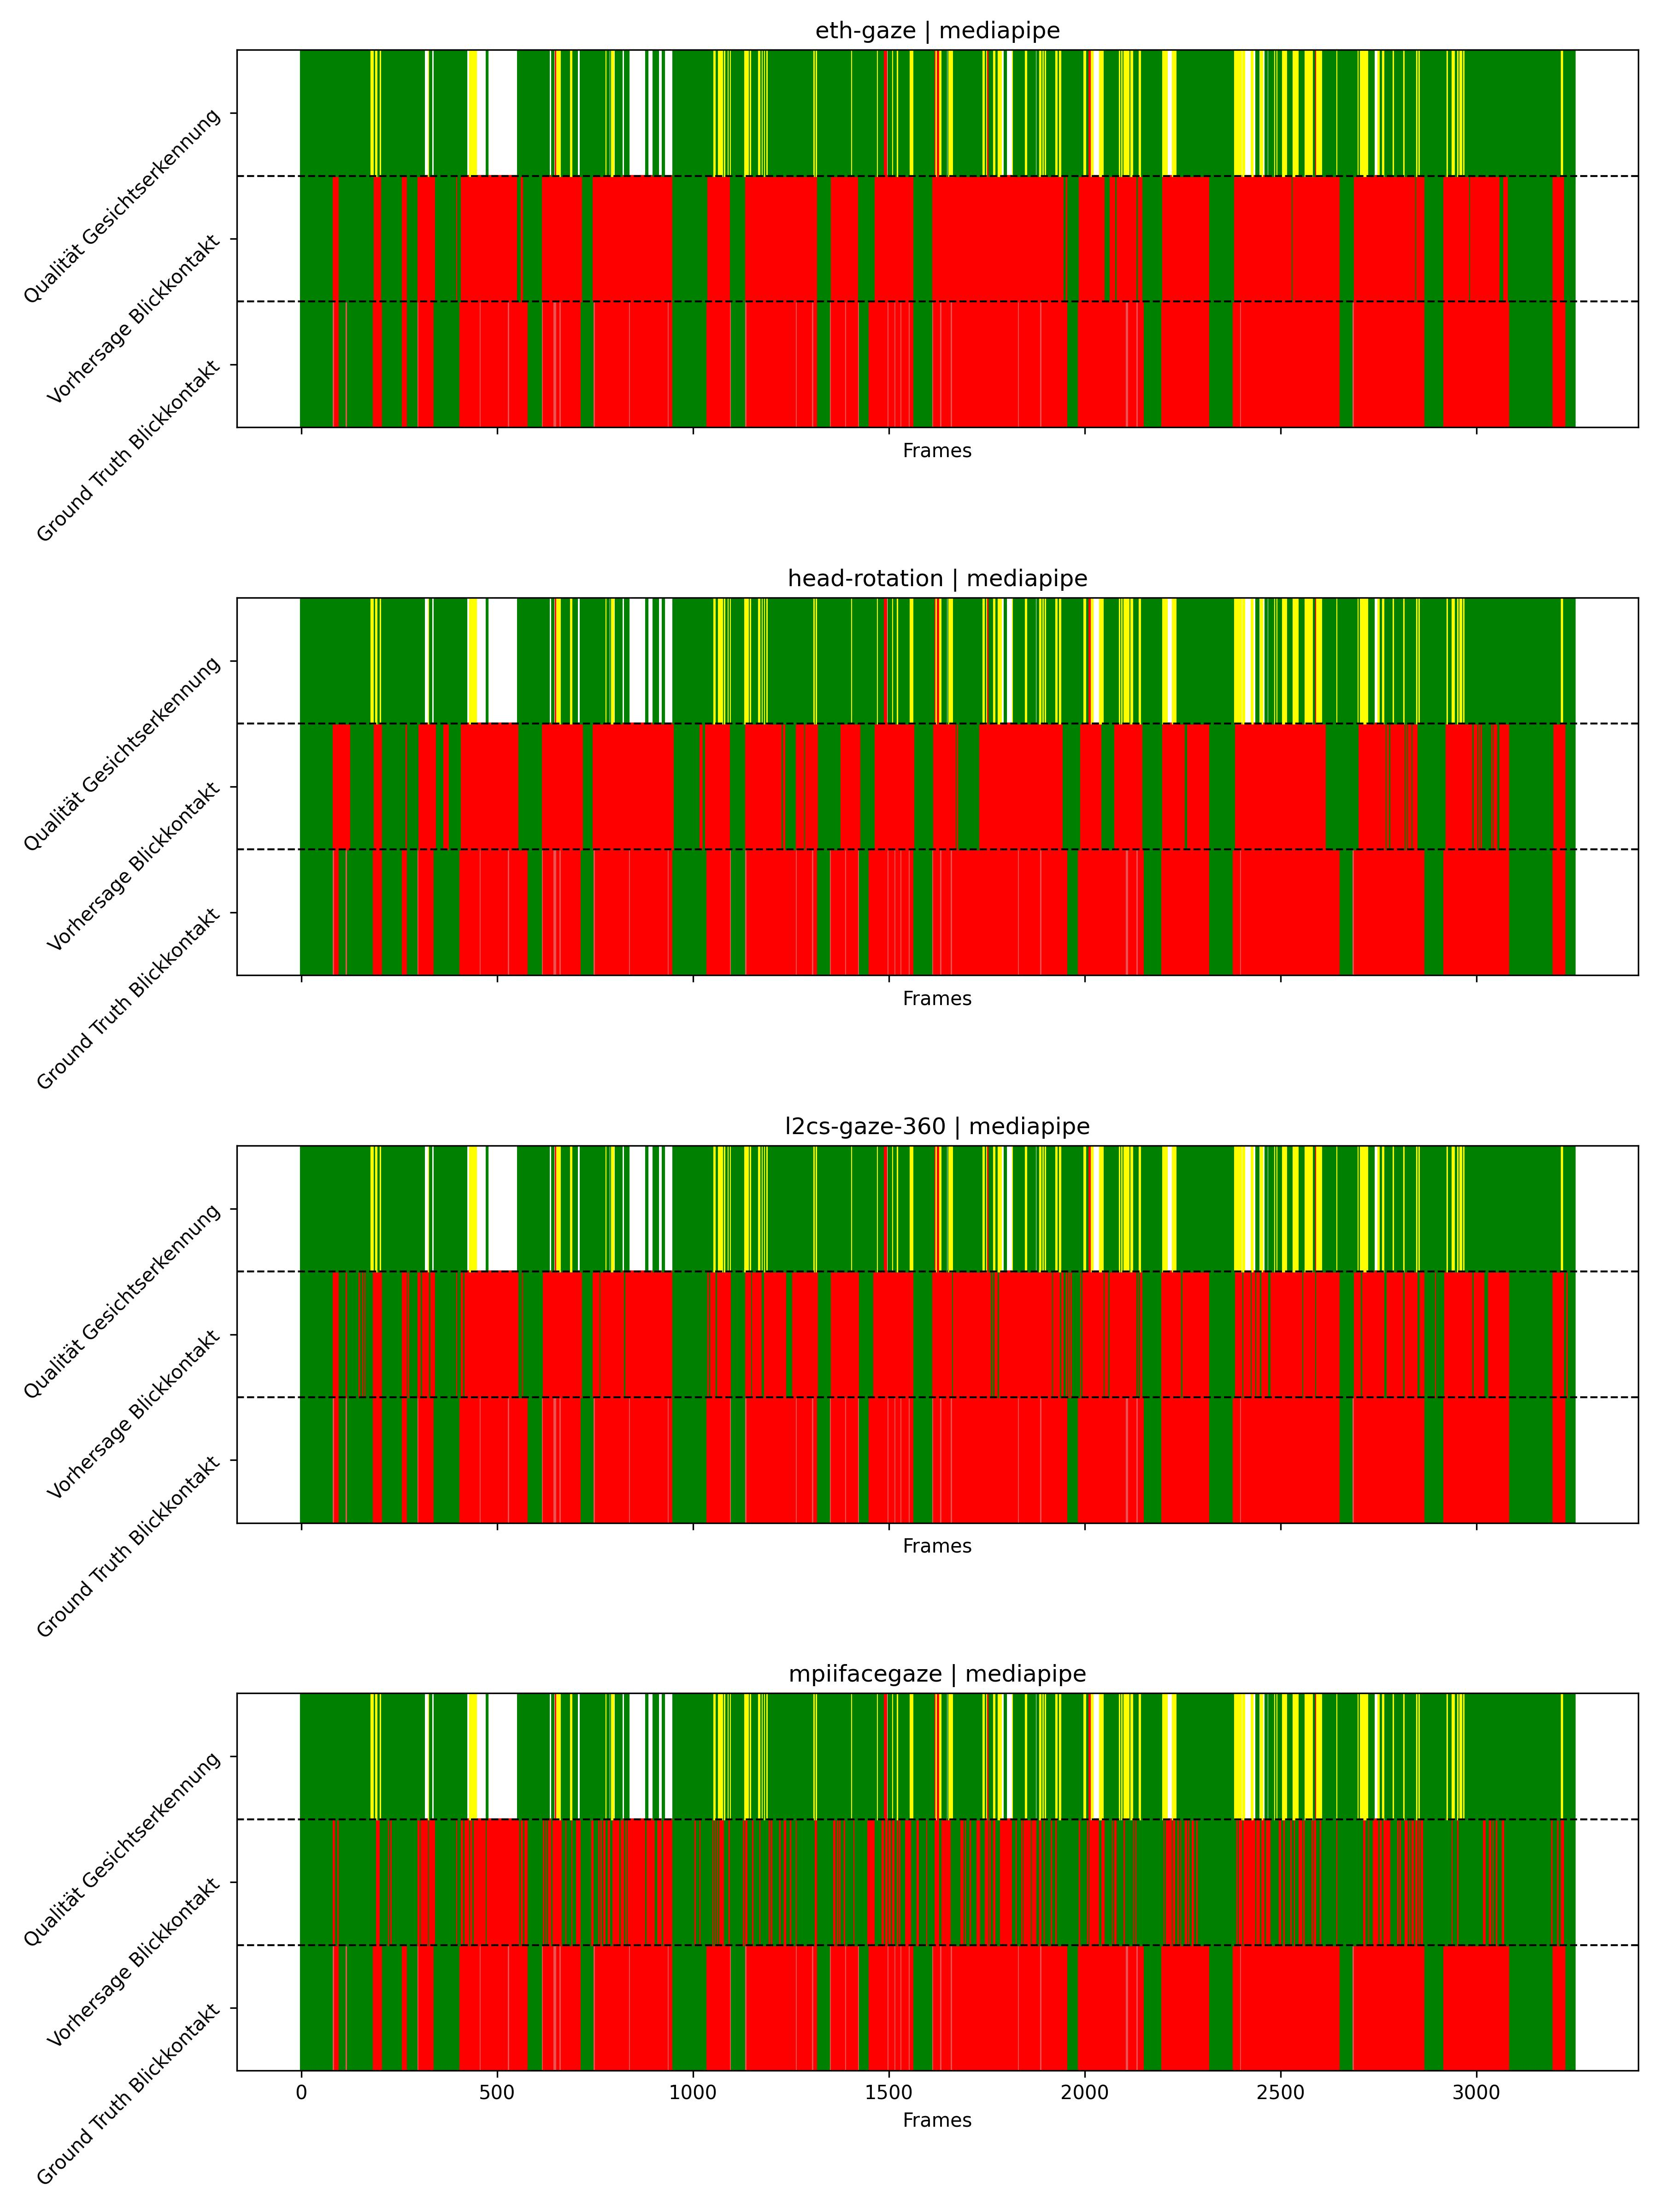
\includegraphics[width=1\linewidth]{appendix/20-mediapipe-overview-gaze.jpg}
\caption{Überblick über die Ground Truth des Blickkontakts, die Vorhersage des Blickkontakts und die Qualität der Gesichtserkennung mit \mediapipe. Die Bedeutung der Farben ist in Abbildung \ref{fig:evaluation:gaze:mpiifacegaze} erklärt.}
\end{figure}

\section{Video 21}
\begin{figure}[H]
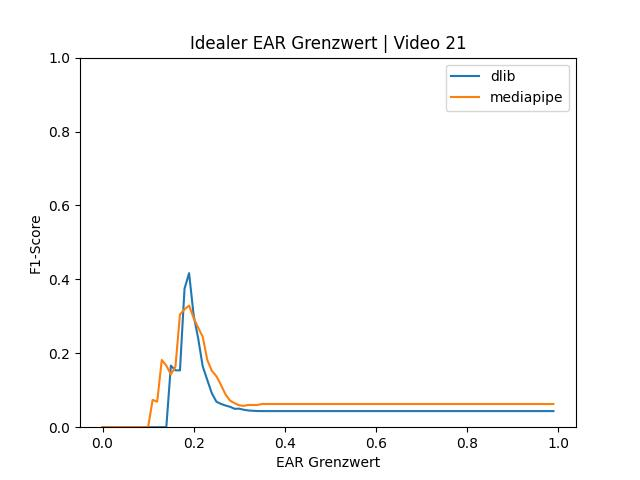
\includegraphics[width=0.7\linewidth]{appendix/21_f1-score-blink.jpg}
\caption{Ergebnisse der Bestimmung des idealen EAR-Grenzwerts für Video 21.}
\end{figure}

\begin{figure}[H]
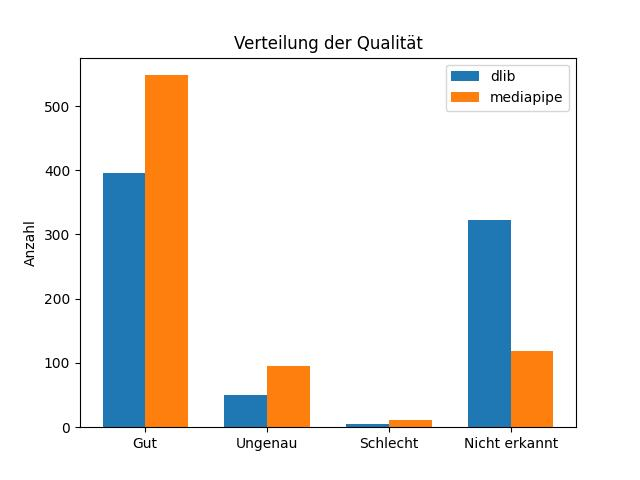
\includegraphics[width=0.7\linewidth]{appendix/21_bar-quality.jpg}
\caption{Aufteilung der Gesichtserkennungsqualität von Video 21.}
\end{figure}

\begin{table}[H]
\centering
\begin{tabular}{l|l|c c |c}
\toprule
\textbf{Gesichtserkennung} & \textbf{Blickrichtung} & \textbf{Seitenlänge} $\hitthresholdsize$ & \textbf{Verschiebung} $\hitthresholdposition$ & \textbf{F1-Score} \\ 
\midrule
\multirow{4}*{dlib}& ETH-XGaze & 0,214 & -0,002 & 0,951  \\ 
& Gaze360 & 0,5 & 0,035 & 0,896 \\ 
& MPIIFaceGaze & 0,082 & -0,039 & 0,872  \\ 
& Kopfrotation & 0,133 & 0,182 & 0,82  \\ 
\hline\multirow{4}*{MediaPipe}& ETH-XGaze & 0,255 & -0,027 & 0,964  \\ 
& Gaze360 & 0,49 & 0,035 & 0,858 \\ 
& MPIIFaceGaze & 0,061 & -0,039 & 0,739  \\ 
& Kopfrotation & 0,122 & 0,157 & 0,874  \\ 
\bottomrule\end{tabular}
\caption{Ergebnis des Hyperparameter-Tunings für die Zone speziell für Video 21.}
\label{tab:appendix:21:local}
\end{table}
\begin{table}[H]
\centering
\begin{tabular}{l|l|c c c c|c c|c}
\toprule
\textbf{Gesichtserkennung} & \textbf{Blickrichtung} & $TP$ & $TN$& $FP$ & $FN$ & \textbf{Precision} & \textbf{Recall} & \textbf{F1-Score} \\ 
\midrule
\multirow{4}*{dlib}& ETH-XGaze & 264 & 473 & 19 & 12 & 0,933 & 0,957 & 0,945 \\ 
& Gaze360 & 252 & 452 & 40 & 24 & 0,863 & 0,913 & 0,887 \\ 
& MPIIFaceGaze & 265 & 370 & 122 & 11 & 0,685 & 0,96 & 0,799 \\ 
& Kopfrotation & 261 & 353 & 139 & 15 & 0,652 & 0,946 & 0,772 \\ 
\hline\multirow{4}*{MediaPipe}& ETH-XGaze & 276 & 464 & 32 & 0 & 0,896 & 1,0 & 0,945 \\ 
& Gaze360 & 225 & 449 & 47 & 51 & 0,827 & 0,815 & 0,821 \\ 
& MPIIFaceGaze & 228 & 280 & 216 & 48 & 0,514 & 0,826 & 0,633 \\ 
& Kopfrotation & 274 & 340 & 156 & 2 & 0,637 & 0,993 & 0,776 \\ 
\bottomrule\end{tabular}
\caption{Zusammensetzung des F1-Scores unter Verwendung der in Kapitel \ref{sec:evaluation:results:gaze:threshold} bestimmten globalen Parameter $\hitthresholdsize$ und $\hitthresholdposition$.}
\label{tab:appendix:21:f1}
\end{table}
\begin{figure}[H]
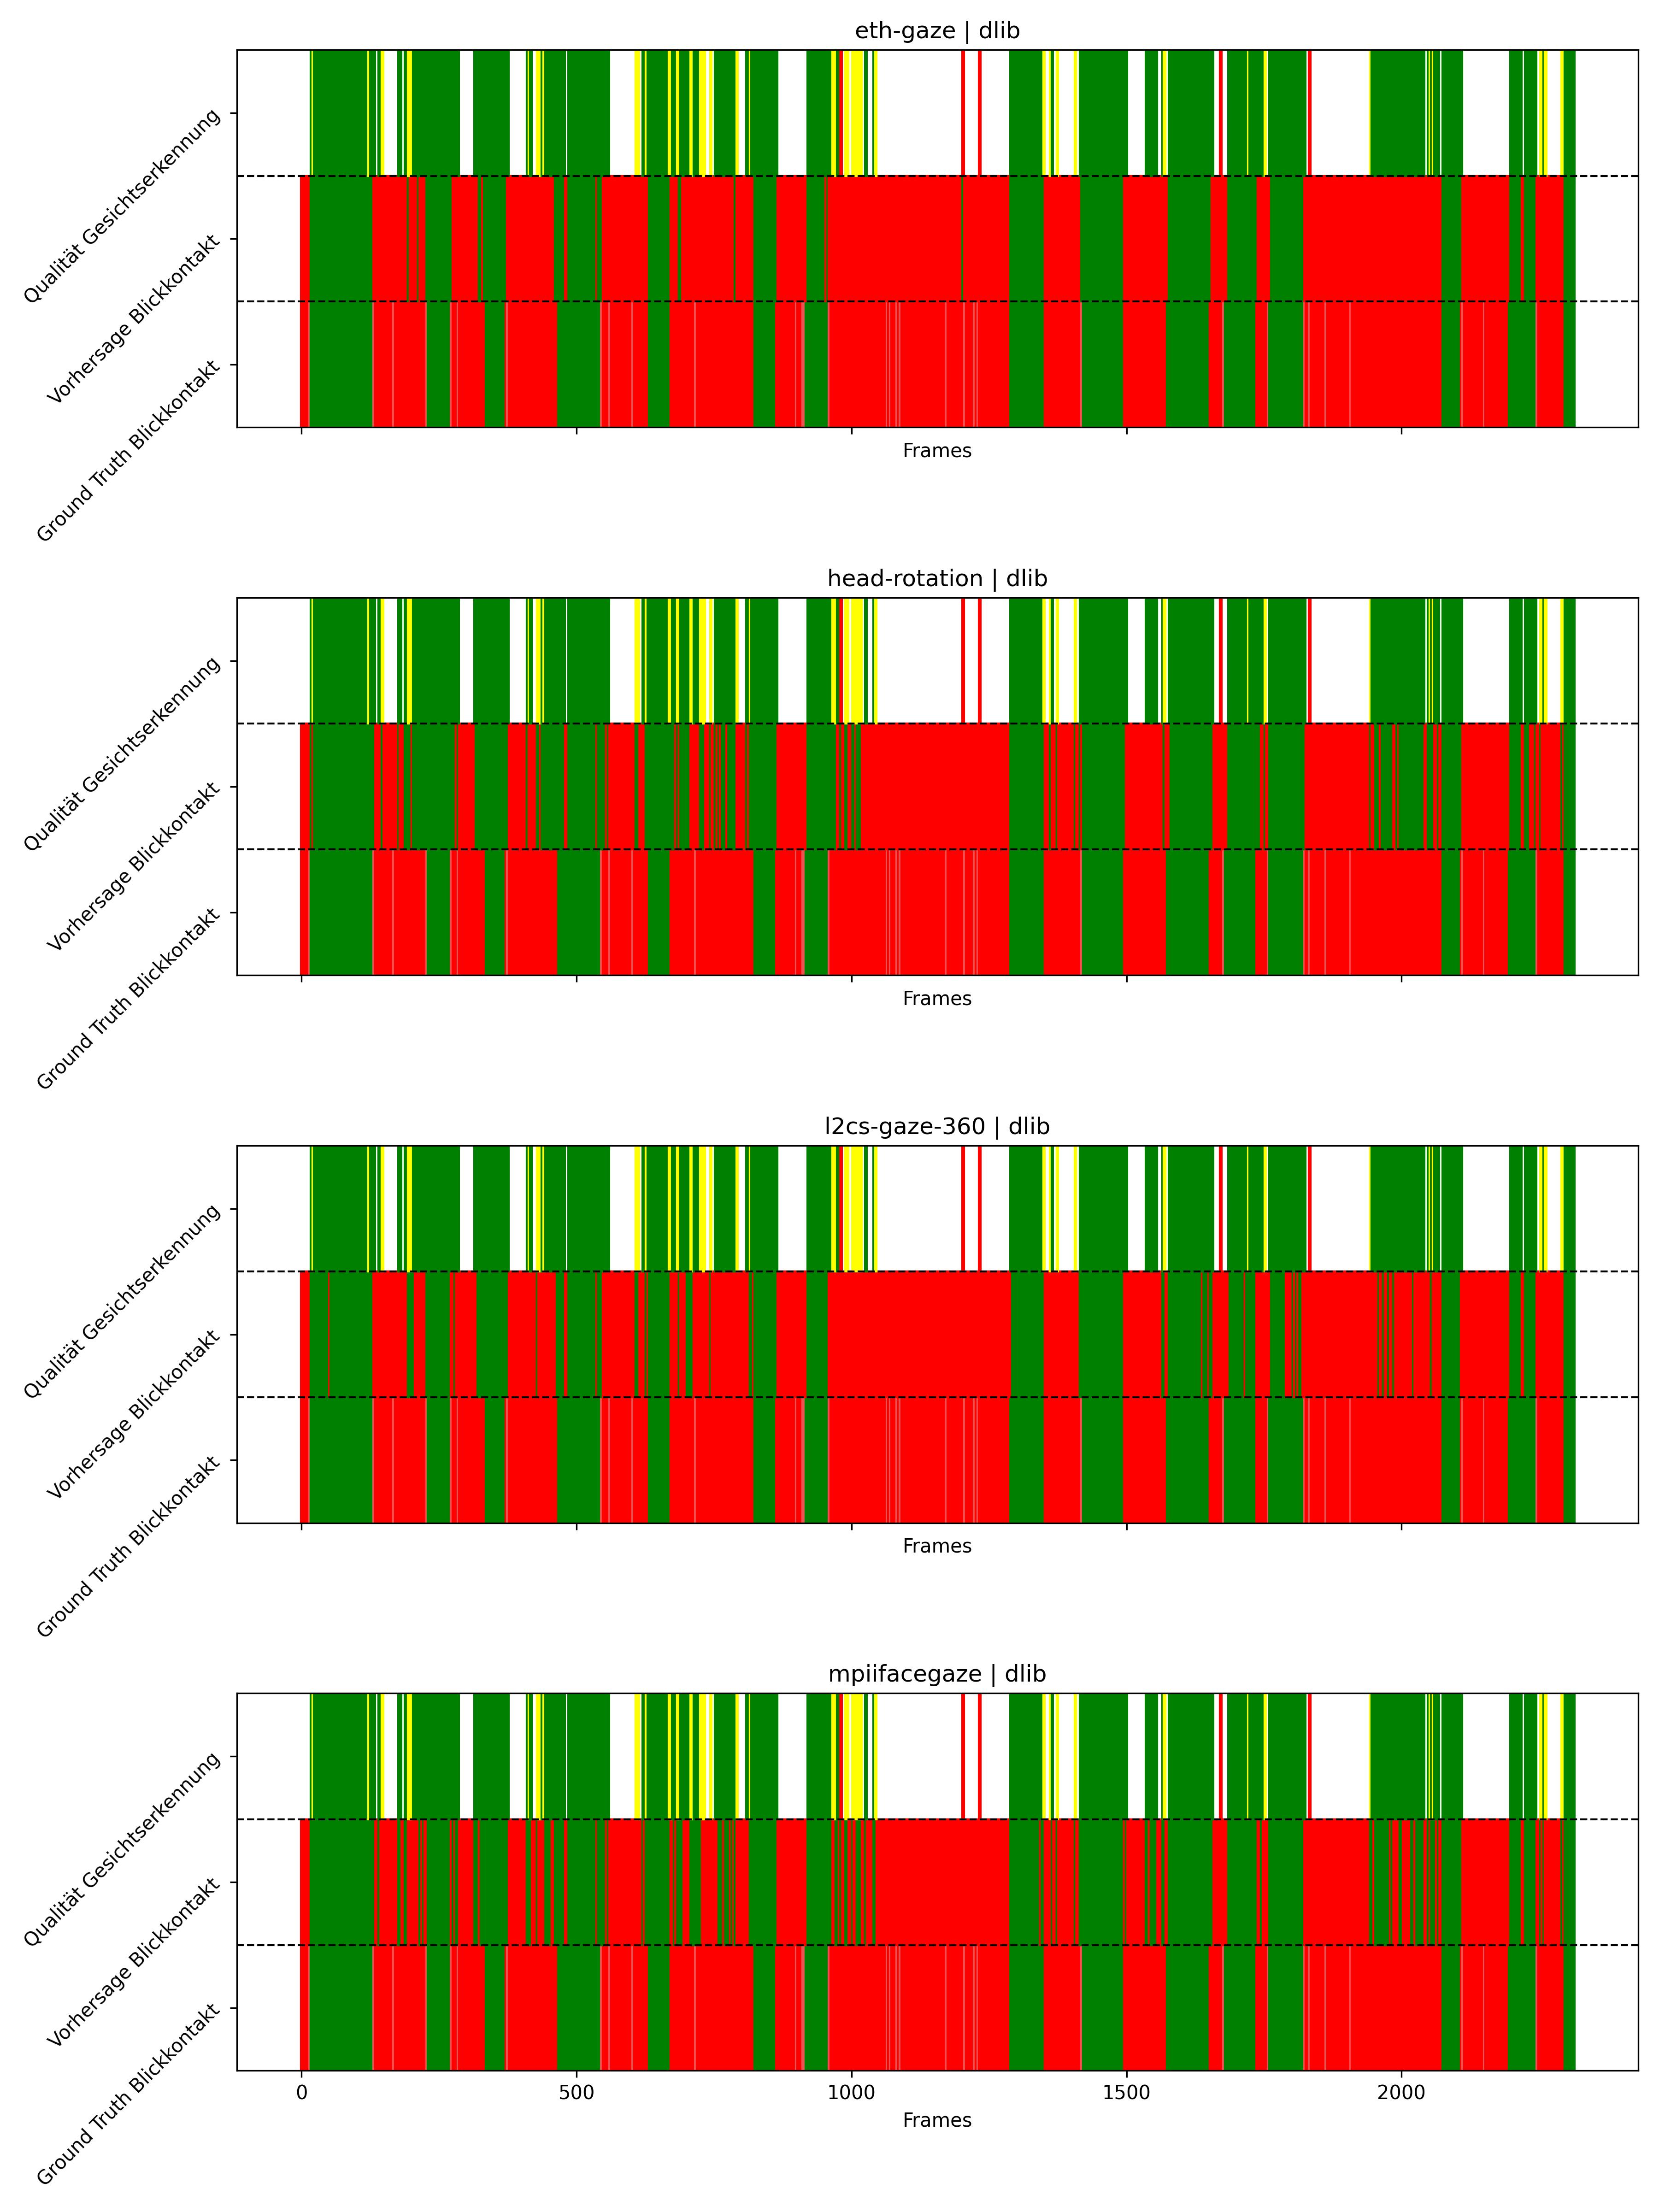
\includegraphics[width=1\linewidth]{appendix/21-dlib-overview-gaze.jpg}
\caption{Überblick über die Ground Truth des Blickkontakts, die Vorhersage des Blickkontakts und die Qualität der Gesichtserkennung mit \dlib. Die Bedeutung der Farben ist in Abbildung \ref{fig:evaluation:gaze:mpiifacegaze} erklärt.  }
\end{figure}

\begin{figure}[H]
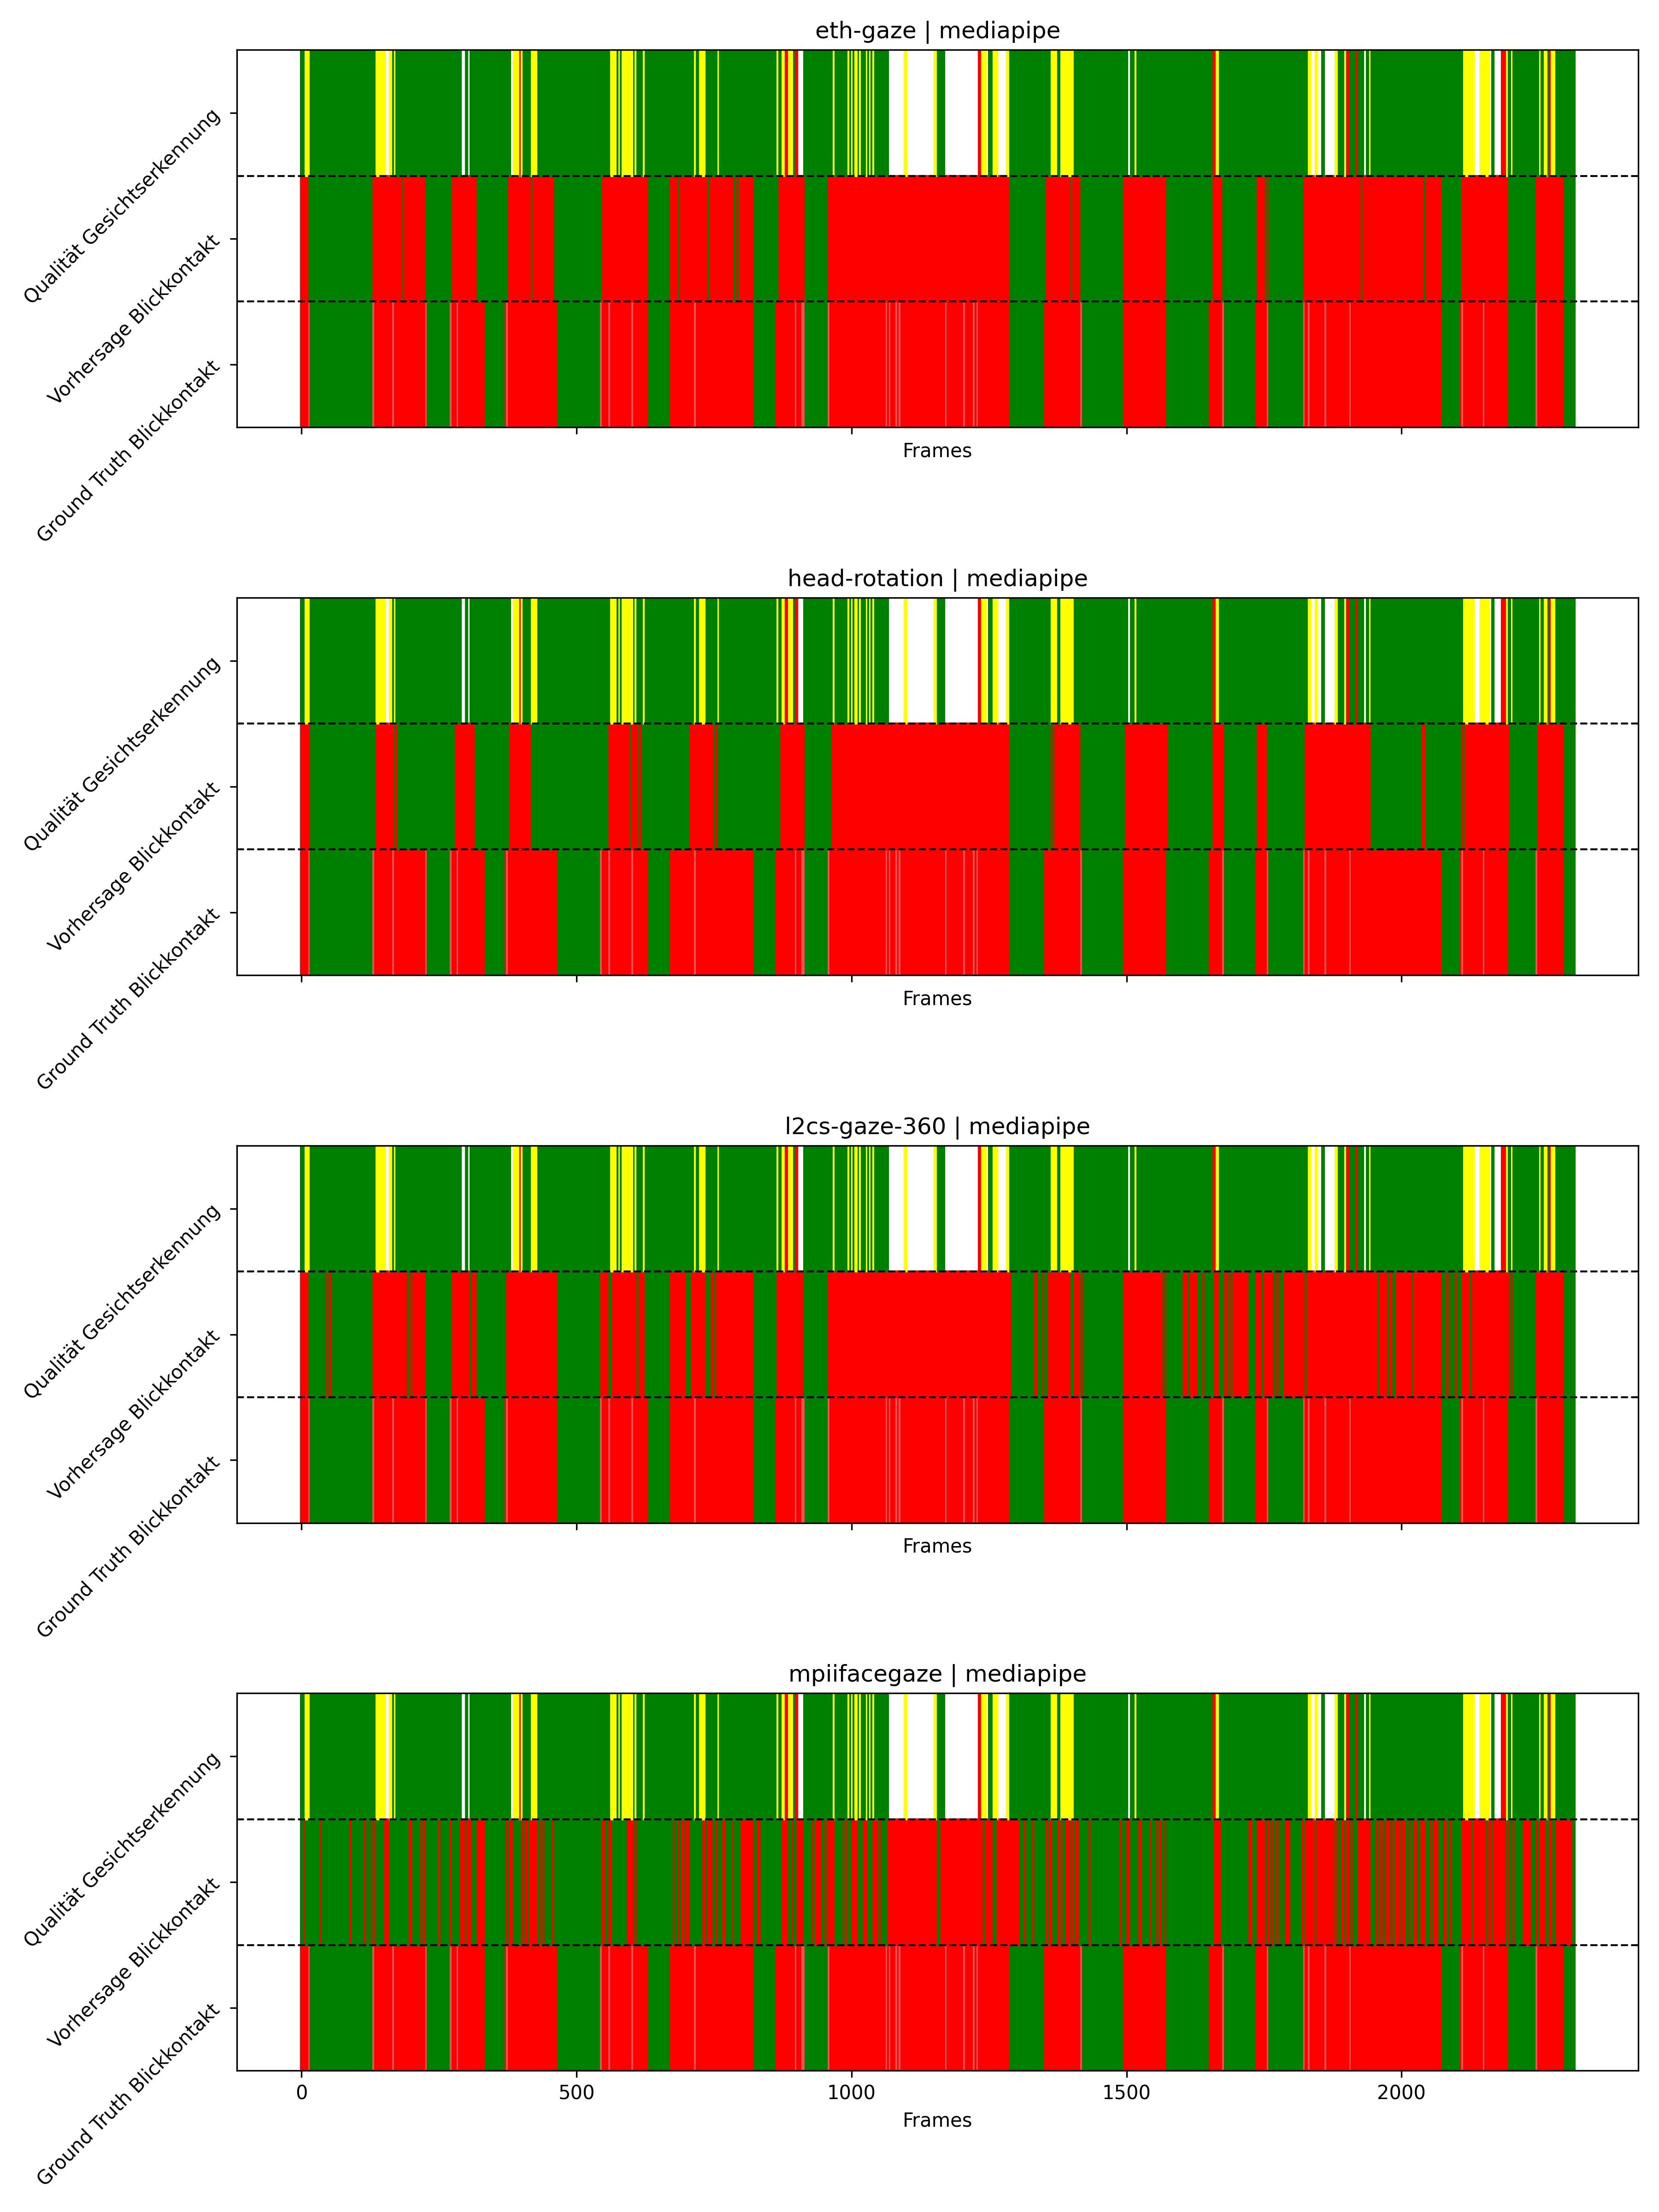
\includegraphics[width=1\linewidth]{appendix/21-mediapipe-overview-gaze.jpg}
\caption{Überblick über die Ground Truth des Blickkontakts, die Vorhersage des Blickkontakts und die Qualität der Gesichtserkennung mit \mediapipe. Die Bedeutung der Farben ist in Abbildung \ref{fig:evaluation:gaze:mpiifacegaze} erklärt.}
\end{figure}

\section{Video 22}
\begin{figure}[H]
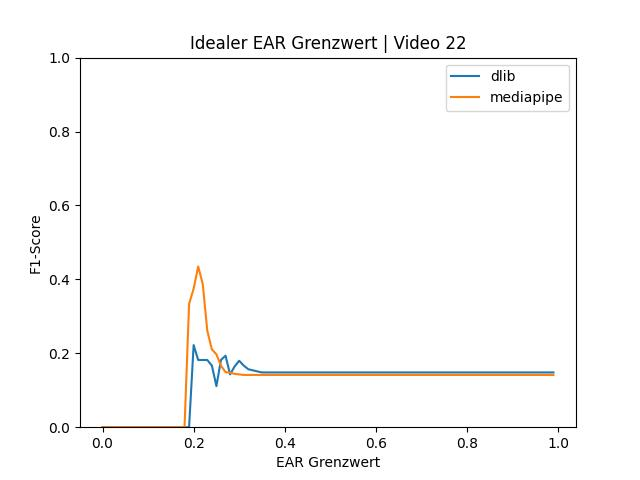
\includegraphics[width=0.7\linewidth]{appendix/22_f1-score-blink.jpg}
\caption{Ergebnisse der Bestimmung des idealen EAR-Grenzwerts für Video 22.}
\end{figure}

\begin{figure}[H]
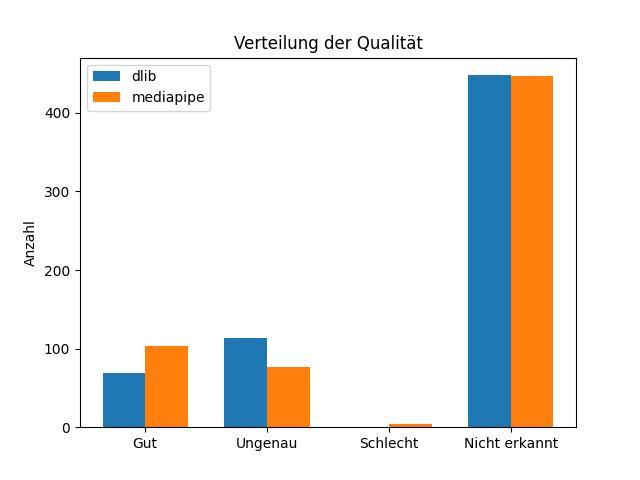
\includegraphics[width=0.7\linewidth]{appendix/22_bar-quality.jpg}
\caption{Aufteilung der Gesichtserkennungsqualität von Video 22.}
\end{figure}

\begin{table}[H]
\centering
\begin{tabular}{l|l|c c |c}
\toprule
\textbf{Gesichtserkennung} & \textbf{Blickrichtung} & \textbf{Seitenlänge} $\hitthresholdsize$ & \textbf{Verschiebung} $\hitthresholdposition$ & \textbf{F1-Score} \\ 
\midrule
\multirow{4}*{dlib}& ETH-XGaze & 0,337 & 0,059 & 0,569  \\ 
& Gaze360 & 0 & 0 & 0 \\ 
& MPIIFaceGaze & 0,112 & 0,059 & 0,51  \\ 
& Kopfrotation & 0,286 & 0,157 & 0,528  \\ 
\hline\multirow{4}*{MediaPipe}& ETH-XGaze & 0,388 & 0,071 & 0,576  \\ 
& Gaze360 & 0 & 0 & 0 \\ 
& MPIIFaceGaze & 0,112 & 0,059 & 0,527  \\ 
& Kopfrotation & 0,245 & 0,133 & 0,625  \\ 
\bottomrule\end{tabular}
\caption{Ergebnis des Hyperparameter-Tunings für die Zone speziell für Video 22.}
\label{tab:appendix:22:local}
\end{table}
\begin{table}[H]
\centering
\begin{tabular}{l|l|c c c c|c c|c}
\toprule
\textbf{Gesichtserkennung} & \textbf{Blickrichtung} & $TP$ & $TN$& $FP$ & $FN$ & \textbf{Precision} & \textbf{Recall} & \textbf{F1-Score} \\ 
\midrule
\multirow{4}*{dlib}& ETH-XGaze & 58 & 462 & 17 & 94 & 0,773 & 0,382 & 0,511 \\ 
& Gaze360 & 0 & 478 & 1 & 152 & 0,0 & 0,0 & 0,0 \\ 
& MPIIFaceGaze & 66 & 390 & 89 & 86 & 0,426 & 0,434 & 0,43 \\ 
& Kopfrotation & 79 & 393 & 86 & 73 & 0,479 & 0,52 & 0,498 \\ 
\hline\multirow{4}*{MediaPipe}& ETH-XGaze & 51 & 462 & 17 & 101 & 0,75 & 0,336 & 0,464 \\ 
& Gaze360 & 0 & 479 & 0 & 152 & 0 & 0,0 & 0,0 \\ 
& MPIIFaceGaze & 49 & 406 & 73 & 103 & 0,402 & 0,322 & 0,358 \\ 
& Kopfrotation & 83 & 434 & 45 & 69 & 0,648 & 0,546 & 0,593 \\ 
\bottomrule\end{tabular}
\caption{Zusammensetzung des F1-Scores unter Verwendung der in Kapitel \ref{sec:evaluation:results:gaze:threshold} bestimmten globalen Parameter $\hitthresholdsize$ und $\hitthresholdposition$.}
\label{tab:appendix:22:f1}
\end{table}
\begin{figure}[H]
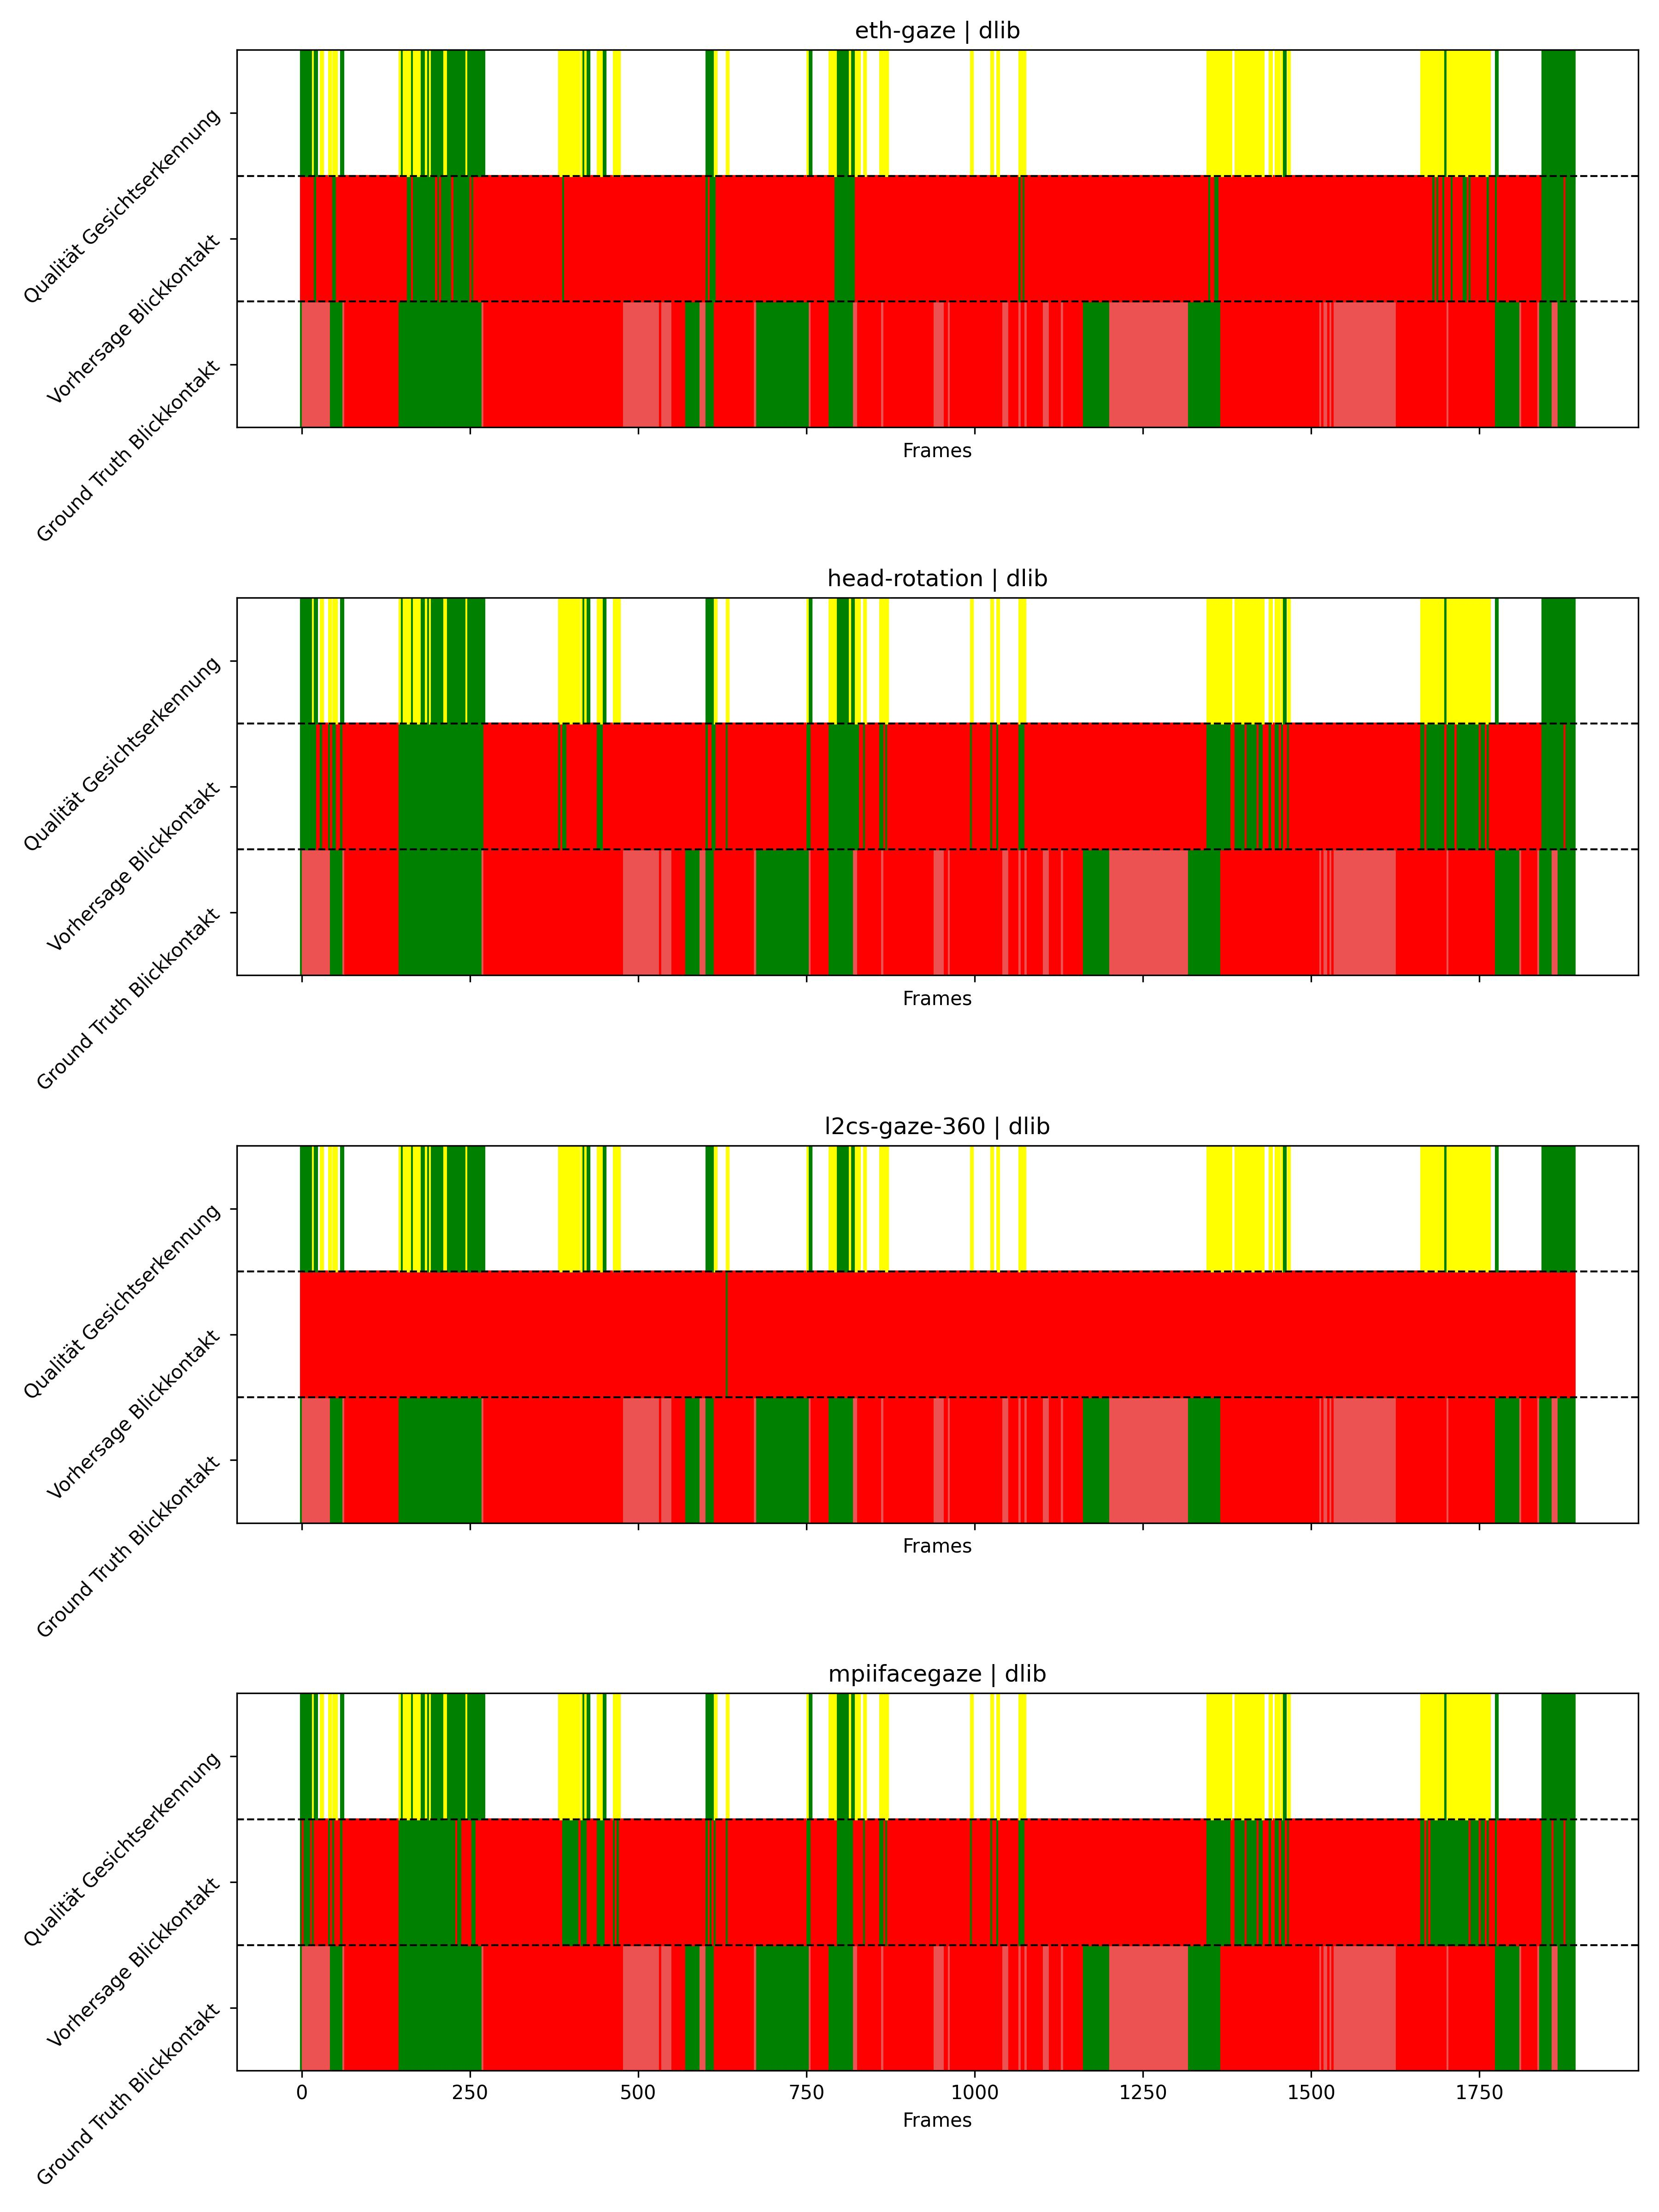
\includegraphics[width=1\linewidth]{appendix/22-dlib-overview-gaze.jpg}
\caption{Überblick über die Ground Truth des Blickkontakts, die Vorhersage des Blickkontakts und die Qualität der Gesichtserkennung mit \dlib. Die Bedeutung der Farben ist in Abbildung \ref{fig:evaluation:gaze:mpiifacegaze} erklärt.  }
\end{figure}

\begin{figure}[H]
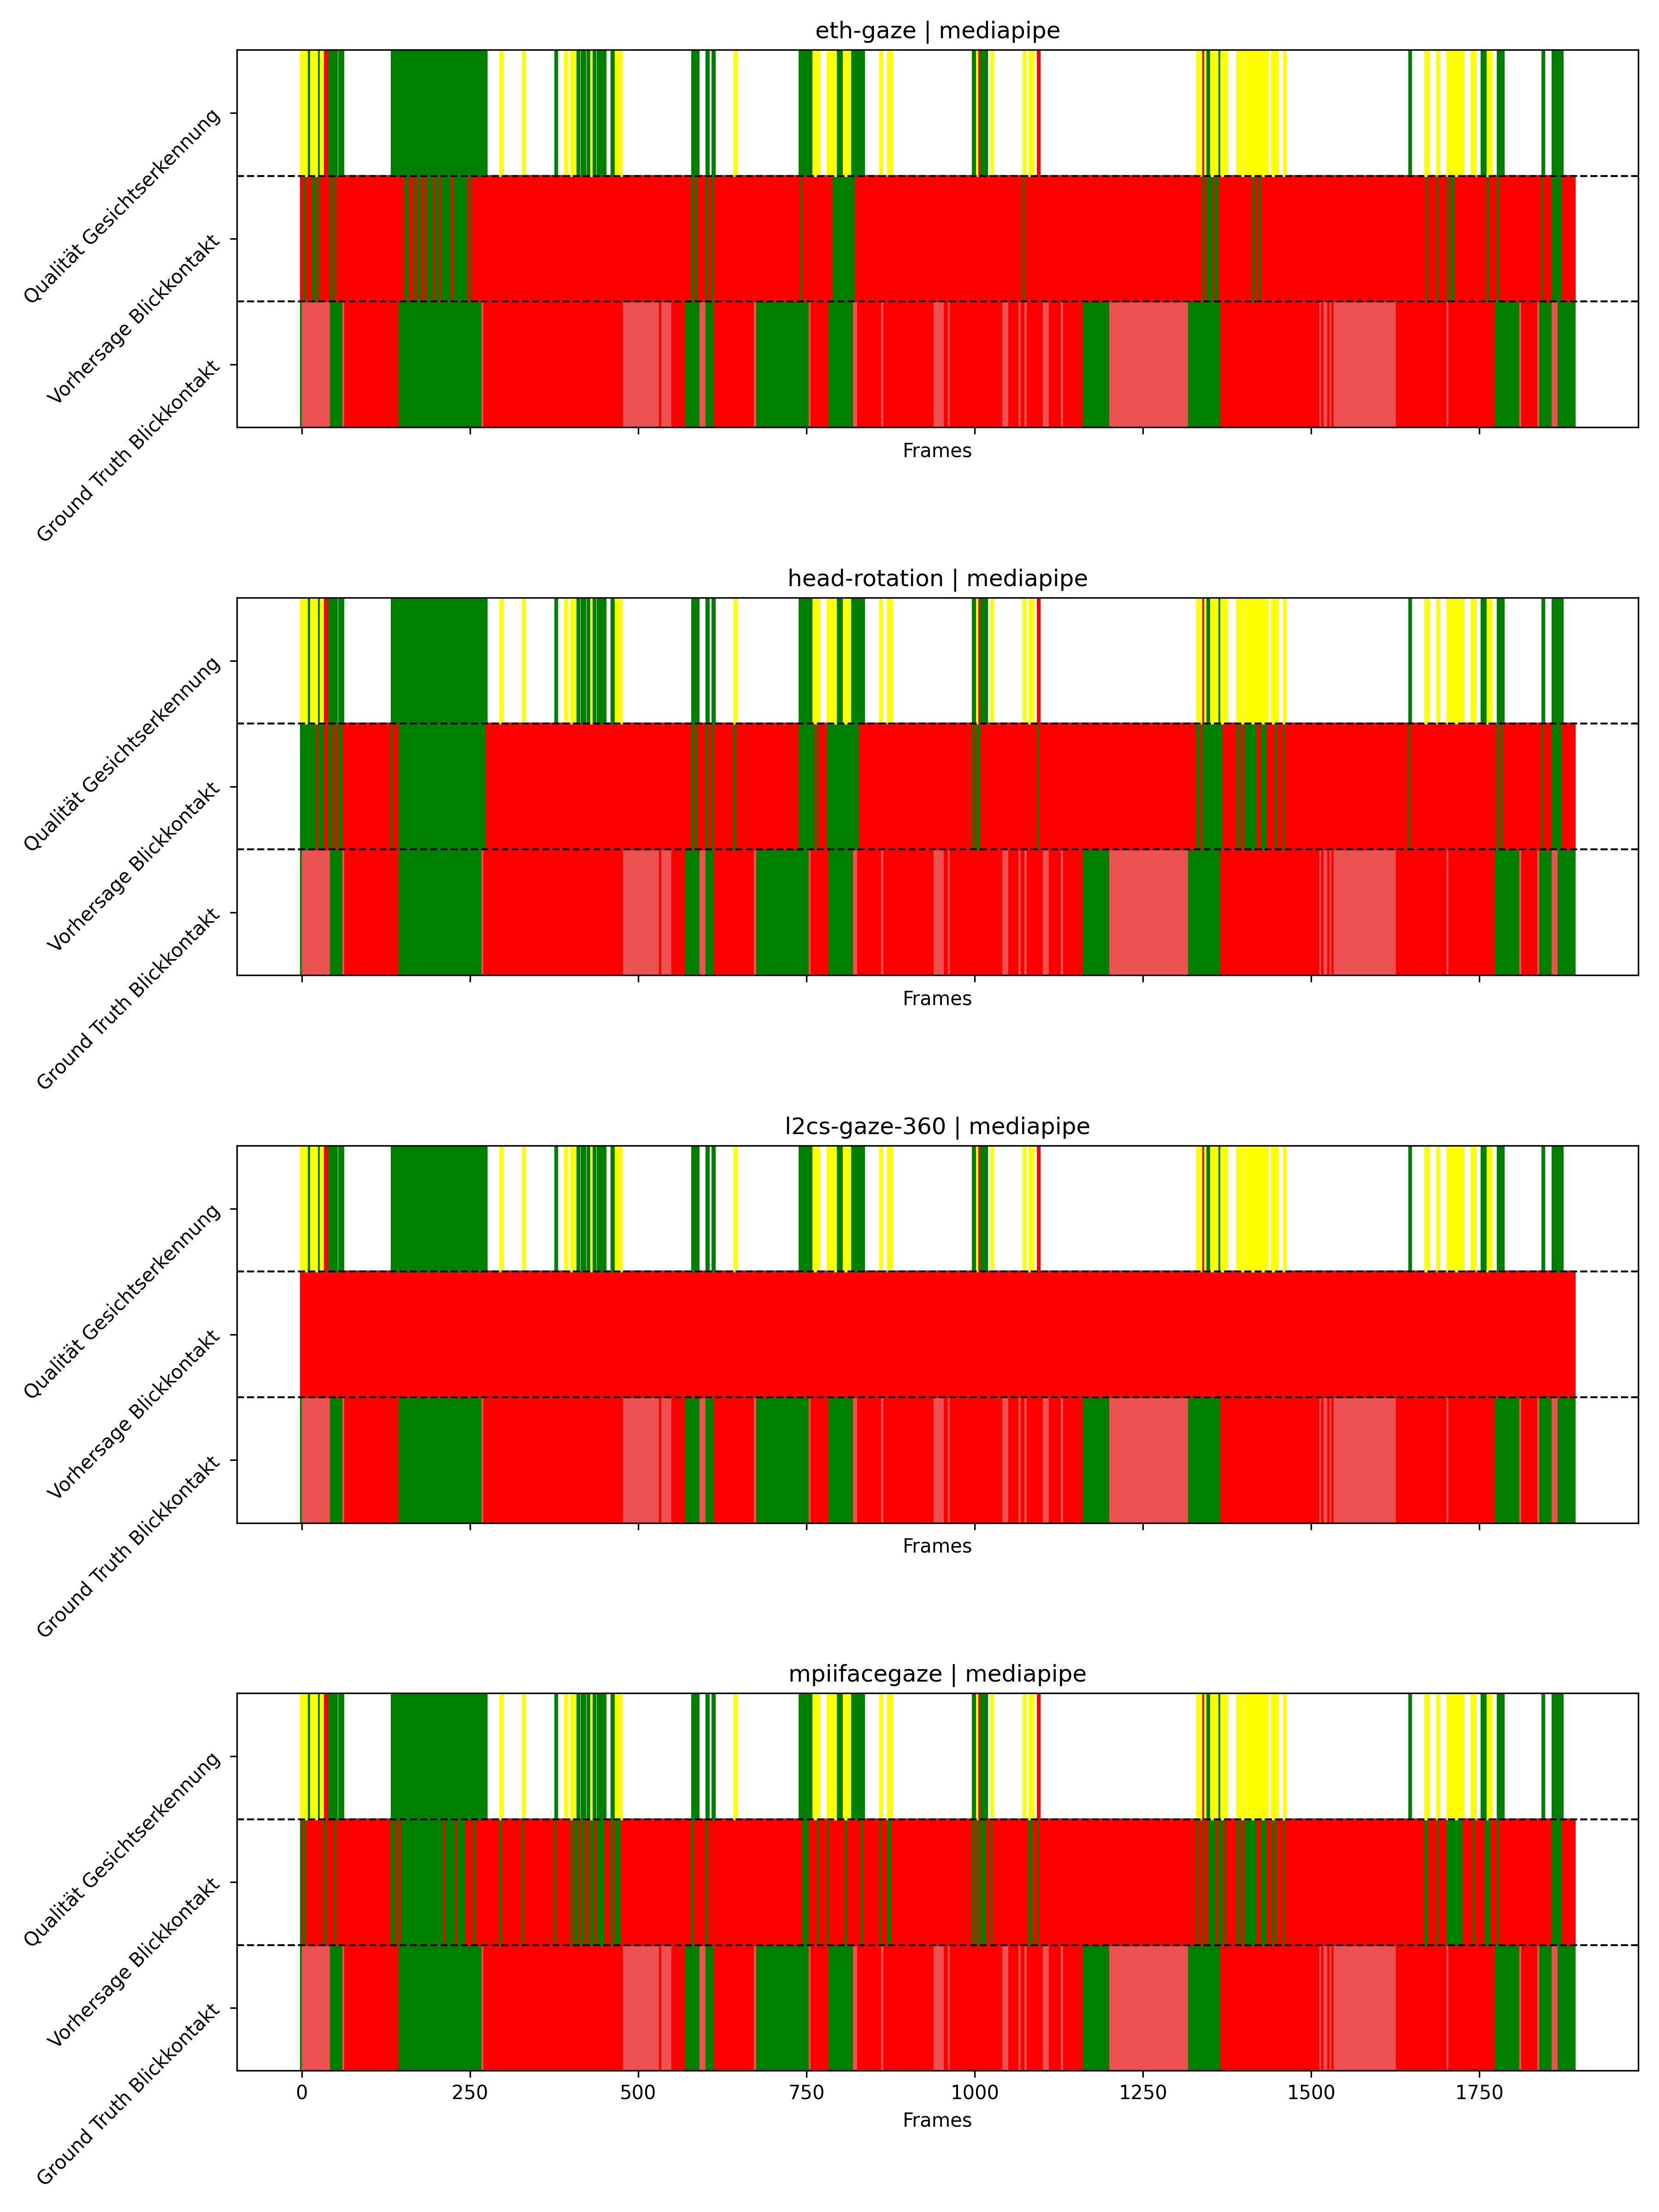
\includegraphics[width=1\linewidth]{appendix/22-mediapipe-overview-gaze.jpg}
\caption{Überblick über die Ground Truth des Blickkontakts, die Vorhersage des Blickkontakts und die Qualität der Gesichtserkennung mit \mediapipe. Die Bedeutung der Farben ist in Abbildung \ref{fig:evaluation:gaze:mpiifacegaze} erklärt.}
\end{figure}

\section{Video 23}
\begin{figure}[H]
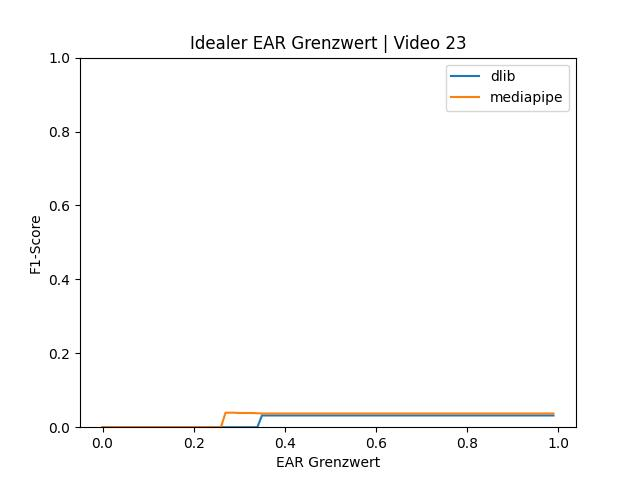
\includegraphics[width=0.7\linewidth]{appendix/23_f1-score-blink.jpg}
\caption{Ergebnisse der Bestimmung des idealen EAR-Grenzwerts für Video 23.}
\end{figure}

\begin{figure}[H]
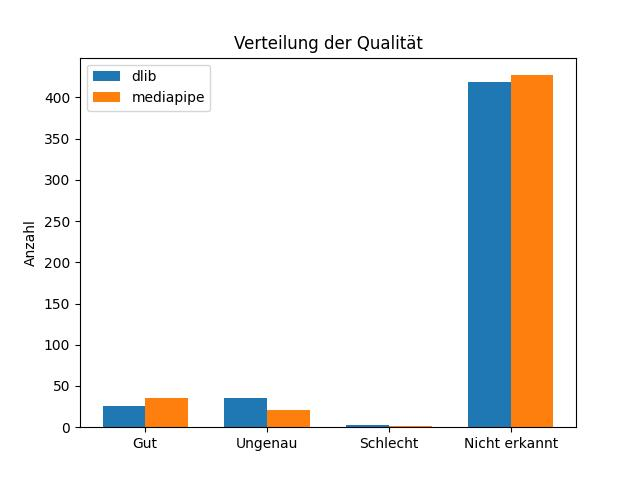
\includegraphics[width=0.7\linewidth]{appendix/23_bar-quality.jpg}
\caption{Aufteilung der Gesichtserkennungsqualität von Video 23.}
\end{figure}

\begin{table}[H]
\centering
\begin{tabular}{l|l|c c |c}
\toprule
\textbf{Gesichtserkennung} & \textbf{Blickrichtung} & \textbf{Seitenlänge} $\hitthresholdsize$ & \textbf{Verschiebung} $\hitthresholdposition$ & \textbf{F1-Score} \\ 
\midrule
\multirow{4}*{dlib}& ETH-XGaze & 0,276 & 0,035 & 0,81  \\ 
& Gaze360 & 0,112 & -0,014 & 0,049 \\ 
& MPIIFaceGaze & 0,163 & 0,12 & 0,783  \\ 
& Kopfrotation & 0,276 & 0,231 & 0,686  \\ 
\hline\multirow{4}*{MediaPipe}& ETH-XGaze & 0,255 & 0,047 & 0,843  \\ 
& Gaze360 & 0,408 & 0,047 & 0,385 \\ 
& MPIIFaceGaze & 0,092 & 0,047 & 0,864  \\ 
& Kopfrotation & 0,122 & 0,243 & 0,864  \\ 
\bottomrule\end{tabular}
\caption{Ergebnis des Hyperparameter-Tunings für die Zone speziell für Video 23.}
\label{tab:appendix:23:local}
\end{table}
\begin{table}[H]
\centering
\begin{tabular}{l|l|c c c c|c c|c}
\toprule
\textbf{Gesichtserkennung} & \textbf{Blickrichtung} & $TP$ & $TN$& $FP$ & $FN$ & \textbf{Precision} & \textbf{Recall} & \textbf{F1-Score} \\ 
\midrule
\multirow{4}*{dlib}& ETH-XGaze & 28 & 436 & 8 & 12 & 0,778 & 0,7 & 0,737 \\ 
& Gaze360 & 1 & 443 & 1 & 39 & 0,5 & 0,025 & 0,048 \\ 
& MPIIFaceGaze & 18 & 420 & 24 & 22 & 0,429 & 0,45 & 0,439 \\ 
& Kopfrotation & 32 & 415 & 29 & 8 & 0,525 & 0,8 & 0,634 \\ 
\hline\multirow{4}*{MediaPipe}& ETH-XGaze & 31 & 439 & 5 & 9 & 0,861 & 0,775 & 0,816 \\ 
& Gaze360 & 9 & 442 & 2 & 31 & 0,818 & 0,225 & 0,353 \\ 
& MPIIFaceGaze & 16 & 427 & 17 & 24 & 0,485 & 0,4 & 0,438 \\ 
& Kopfrotation & 33 & 437 & 7 & 7 & 0,825 & 0,825 & 0,825 \\ 
\bottomrule\end{tabular}
\caption{Zusammensetzung des F1-Scores unter Verwendung der in Kapitel \ref{sec:evaluation:results:gaze:threshold} bestimmten globalen Parameter $\hitthresholdsize$ und $\hitthresholdposition$.}
\label{tab:appendix:23:f1}
\end{table}
\begin{figure}[H]
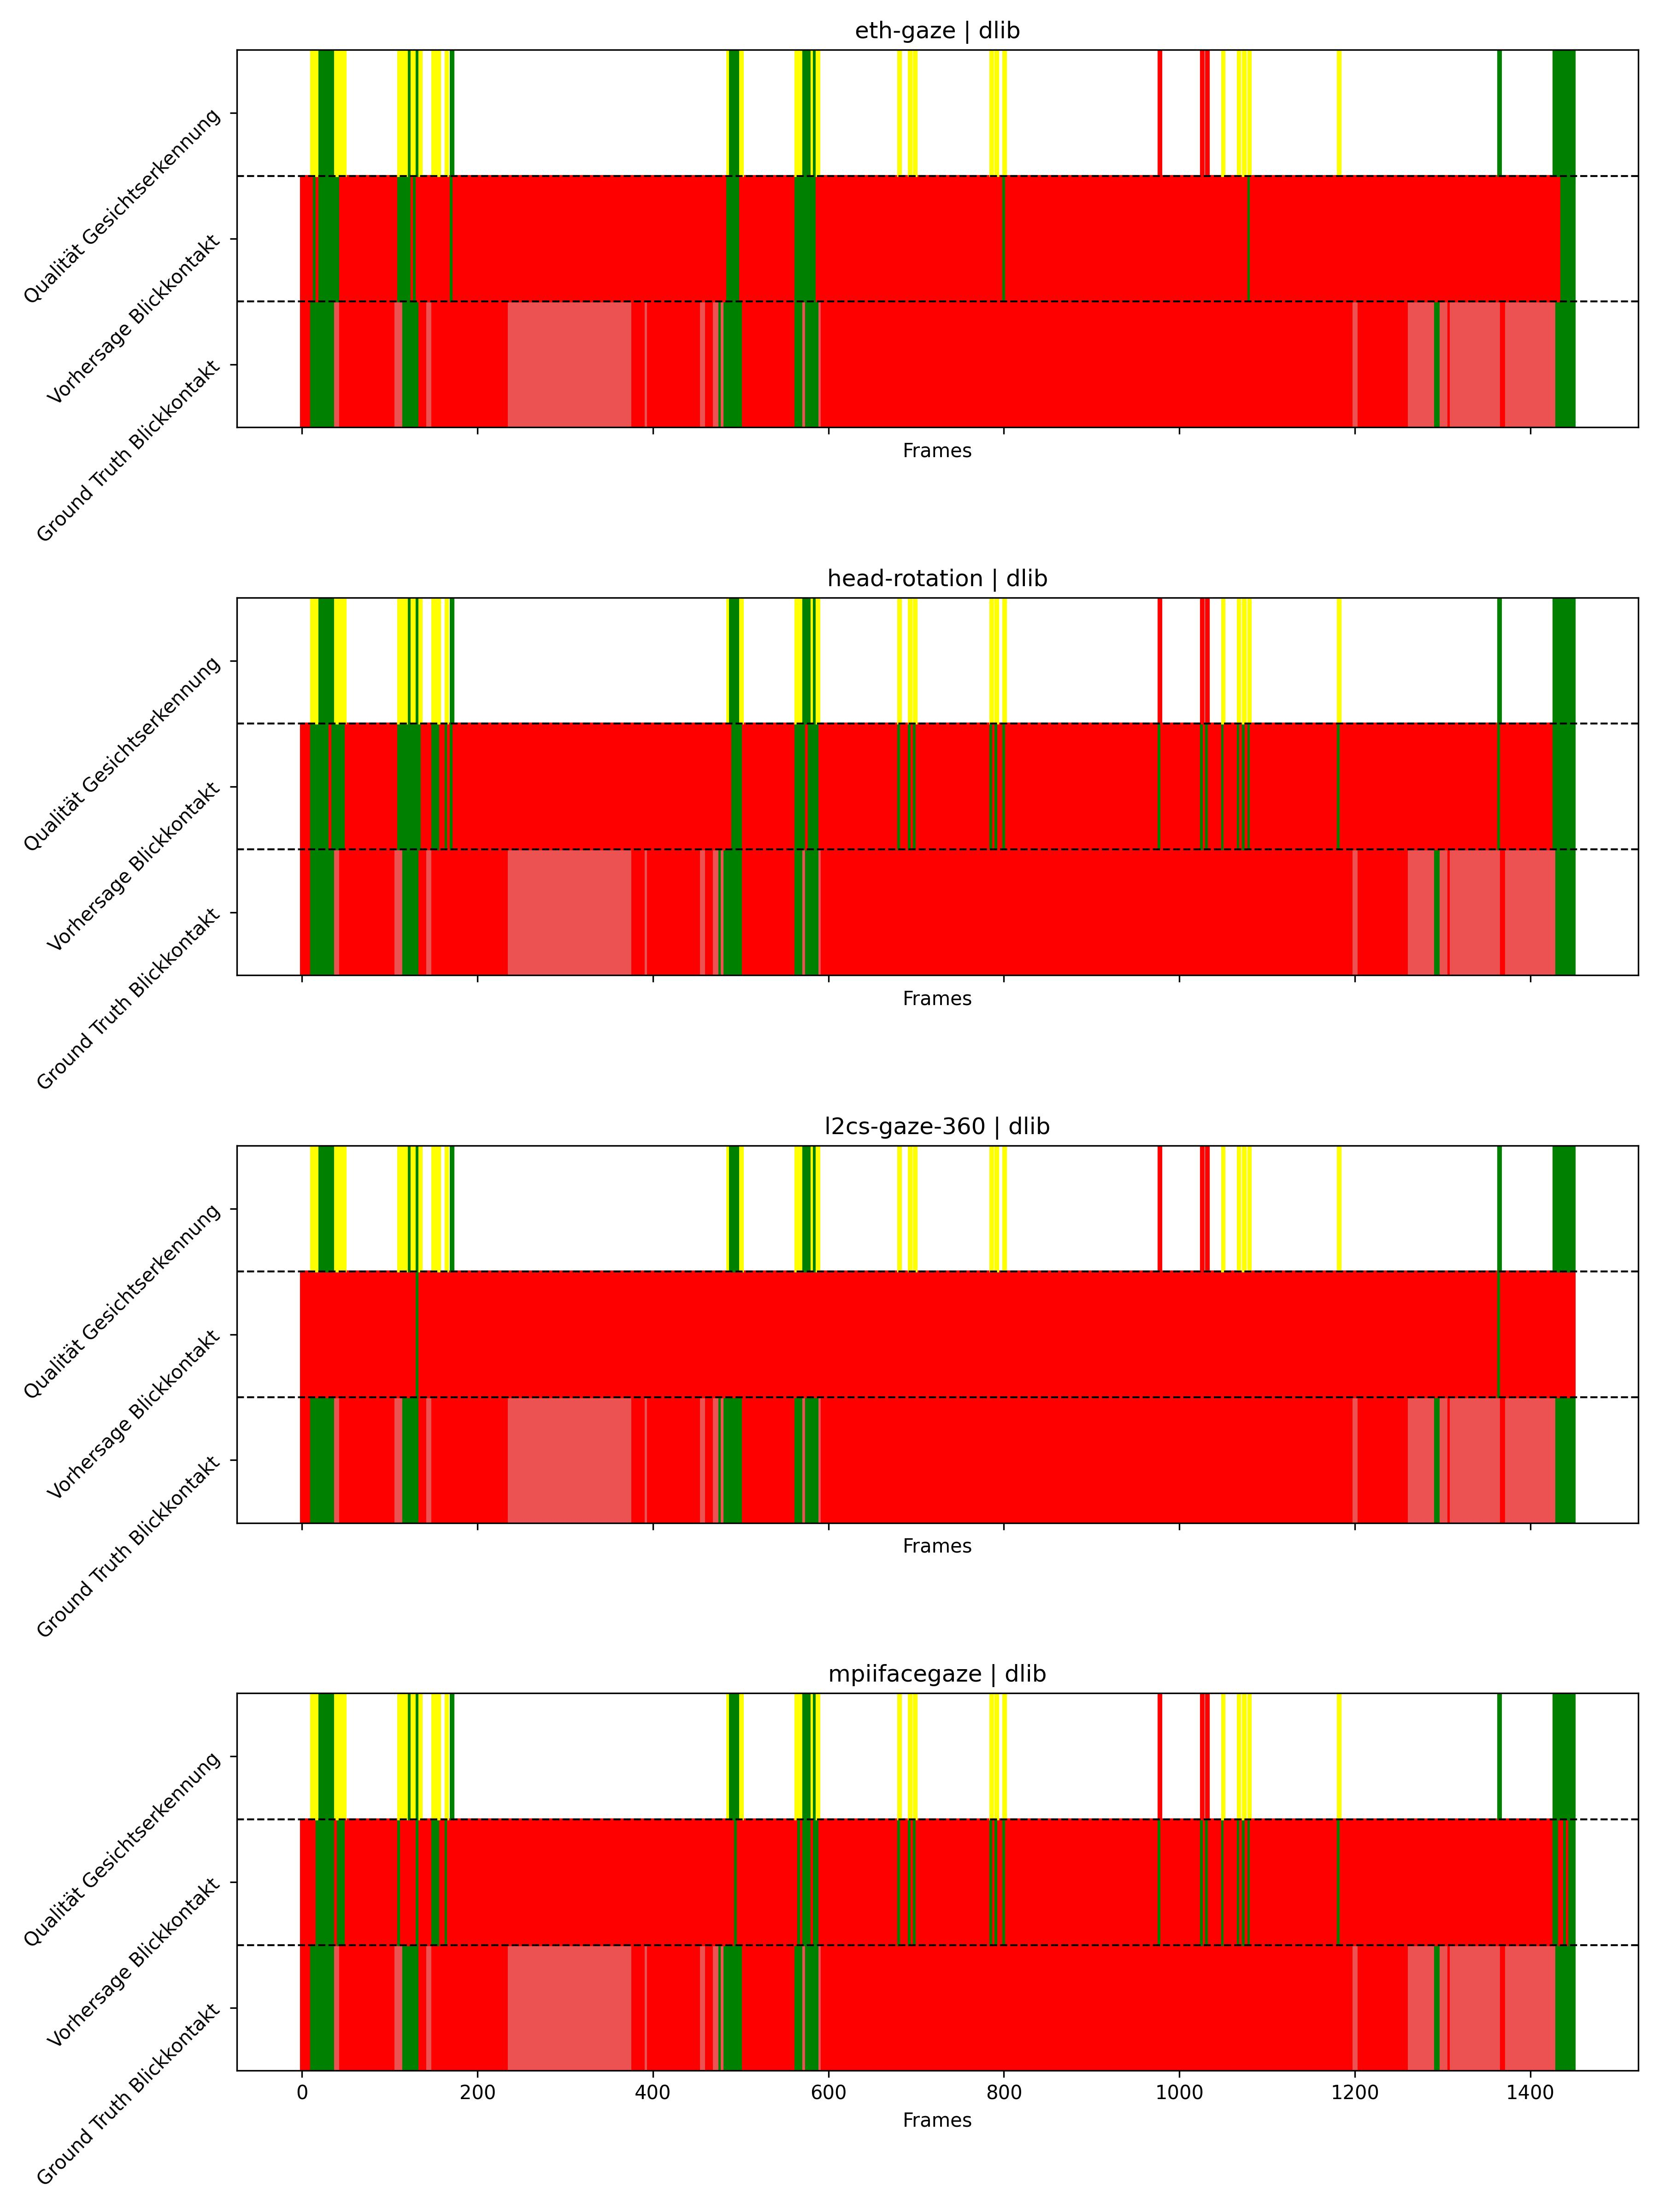
\includegraphics[width=1\linewidth]{appendix/23-dlib-overview-gaze.jpg}
\caption{Überblick über die Ground Truth des Blickkontakts, die Vorhersage des Blickkontakts und die Qualität der Gesichtserkennung mit \dlib. Die Bedeutung der Farben ist in Abbildung \ref{fig:evaluation:gaze:mpiifacegaze} erklärt.  }
\end{figure}

\begin{figure}[H]
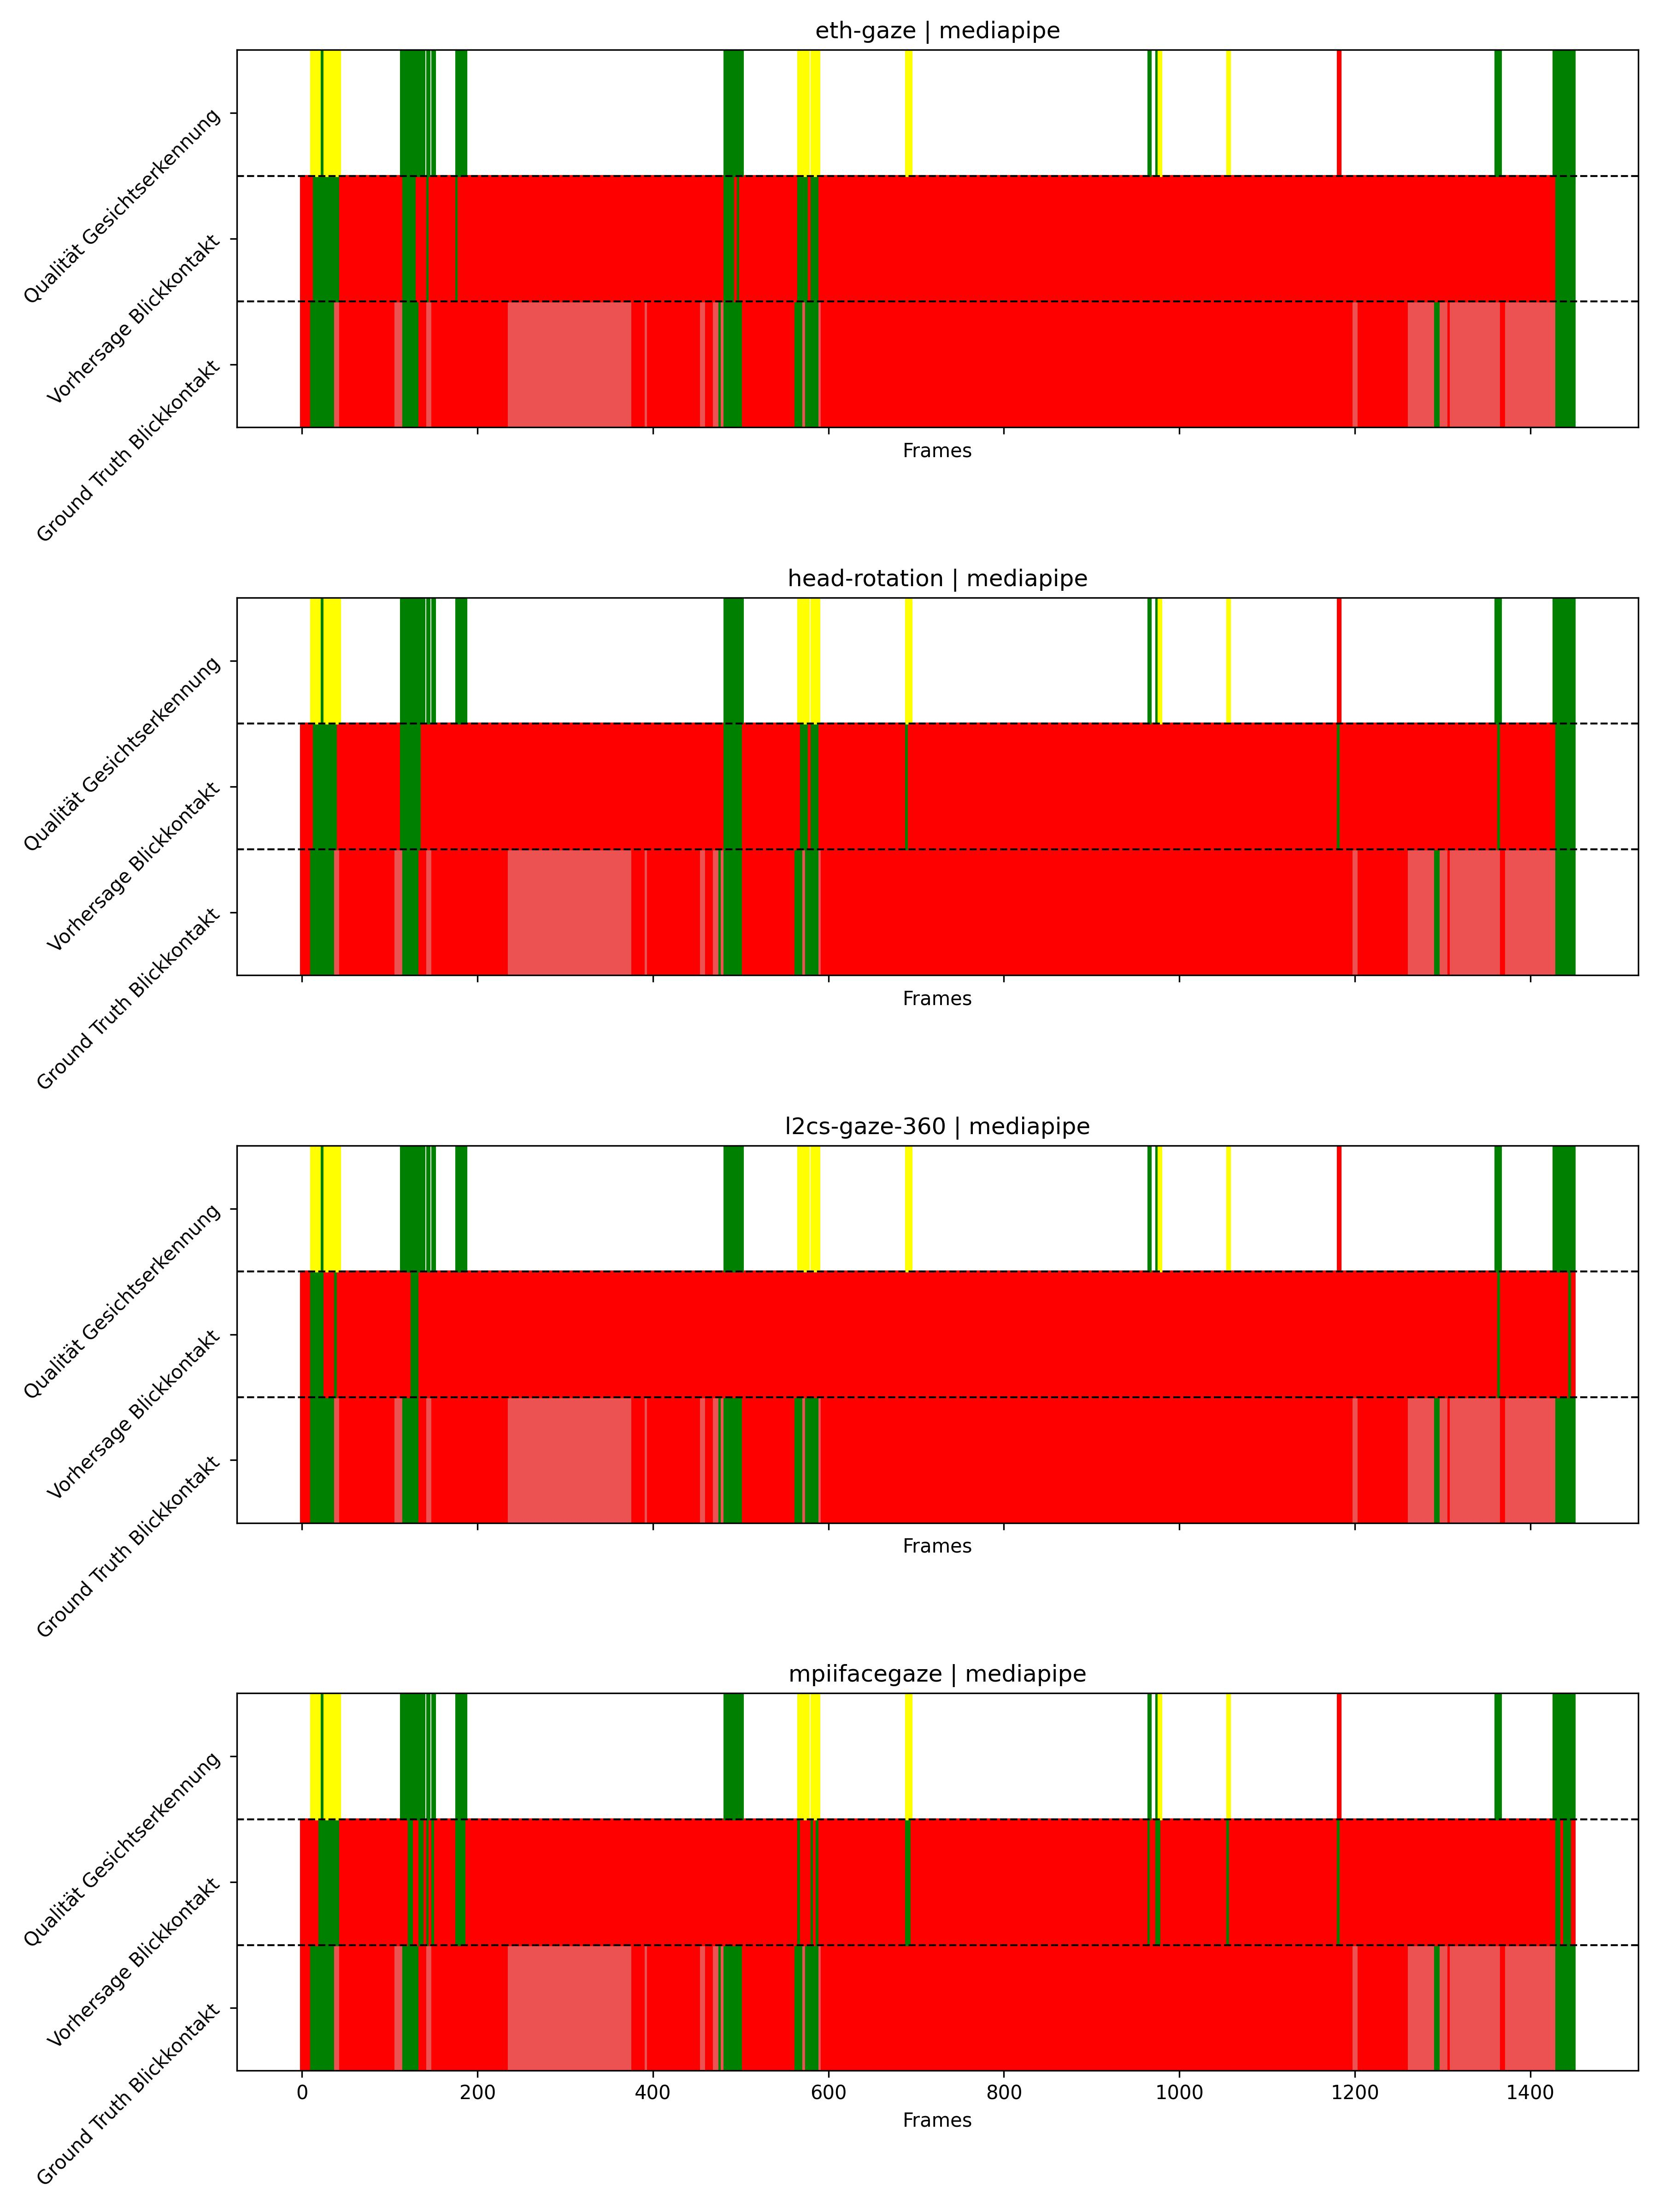
\includegraphics[width=1\linewidth]{appendix/23-mediapipe-overview-gaze.jpg}
\caption{Überblick über die Ground Truth des Blickkontakts, die Vorhersage des Blickkontakts und die Qualität der Gesichtserkennung mit \mediapipe. Die Bedeutung der Farben ist in Abbildung \ref{fig:evaluation:gaze:mpiifacegaze} erklärt.}
\end{figure}

\section{Video 24}
\begin{figure}[H]
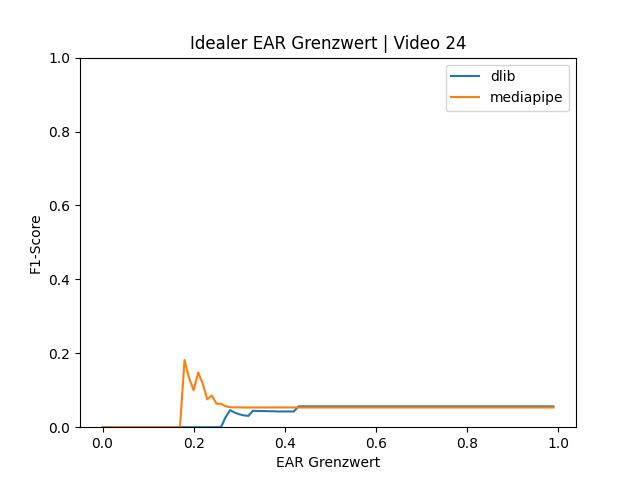
\includegraphics[width=0.7\linewidth]{appendix/24_f1-score-blink.jpg}
\caption{Ergebnisse der Bestimmung des idealen EAR-Grenzwerts für Video 24.}
\end{figure}

\begin{figure}[H]
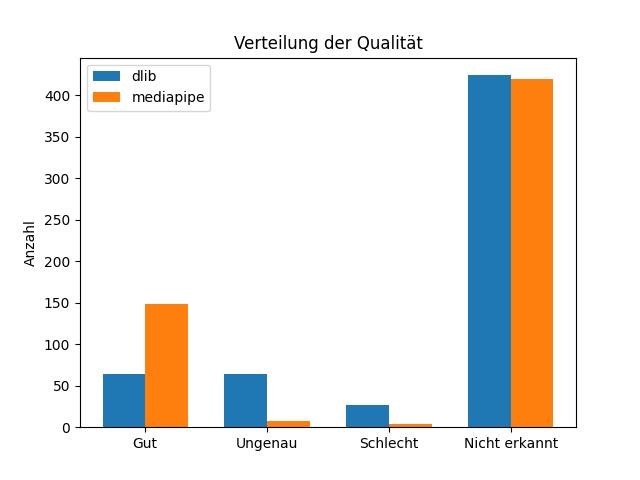
\includegraphics[width=0.7\linewidth]{appendix/24_bar-quality.jpg}
\caption{Aufteilung der Gesichtserkennungsqualität von Video 24.}
\end{figure}

\begin{table}[H]
\centering
\begin{tabular}{l|l|c c |c}
\toprule
\textbf{Gesichtserkennung} & \textbf{Blickrichtung} & \textbf{Seitenlänge} $\hitthresholdsize$ & \textbf{Verschiebung} $\hitthresholdposition$ & \textbf{F1-Score} \\ 
\midrule
\multirow{4}*{dlib}& ETH-XGaze & 0,418 & 0,071 & 0,899  \\ 
& Gaze360 & 0,5 & 0,047 & 0,782 \\ 
& MPIIFaceGaze & 0,122 & 0,071 & 0,8  \\ 
& Kopfrotation & 0,255 & 0,206 & 0,817  \\ 
\hline\multirow{4}*{MediaPipe}& ETH-XGaze & 0,449 & 0,047 & 0,839  \\ 
& Gaze360 & 0,5 & 0,035 & 0,601 \\ 
& MPIIFaceGaze & 0,092 & 0,047 & 0,759  \\ 
& Kopfrotation & 0,122 & 0,218 & 0,834  \\ 
\bottomrule\end{tabular}
\caption{Ergebnis des Hyperparameter-Tunings für die Zone speziell für Video 24.}
\label{tab:appendix:24:local}
\end{table}
\begin{table}[H]
\centering
\begin{tabular}{l|l|c c c c|c c|c}
\toprule
\textbf{Gesichtserkennung} & \textbf{Blickrichtung} & $TP$ & $TN$& $FP$ & $FN$ & \textbf{Precision} & \textbf{Recall} & \textbf{F1-Score} \\ 
\midrule
\multirow{4}*{dlib}& ETH-XGaze & 92 & 455 & 10 & 22 & 0,902 & 0,807 & 0,852 \\ 
& Gaze360 & 77 & 459 & 6 & 37 & 0,928 & 0,675 & 0,782 \\ 
& MPIIFaceGaze & 62 & 429 & 36 & 52 & 0,633 & 0,544 & 0,585 \\ 
& Kopfrotation & 107 & 424 & 41 & 7 & 0,723 & 0,939 & 0,817 \\ 
\hline\multirow{4}*{MediaPipe}& ETH-XGaze & 83 & 455 & 10 & 31 & 0,892 & 0,728 & 0,802 \\ 
& Gaze360 & 49 & 459 & 6 & 65 & 0,891 & 0,43 & 0,58 \\ 
& MPIIFaceGaze & 45 & 421 & 44 & 69 & 0,506 & 0,395 & 0,443 \\ 
& Kopfrotation & 88 & 453 & 12 & 26 & 0,88 & 0,772 & 0,822 \\ 
\bottomrule\end{tabular}
\caption{Zusammensetzung des F1-Scores unter Verwendung der in Kapitel \ref{sec:evaluation:results:gaze:threshold} bestimmten globalen Parameter $\hitthresholdsize$ und $\hitthresholdposition$.}
\label{tab:appendix:24:f1}
\end{table}
\begin{figure}[H]
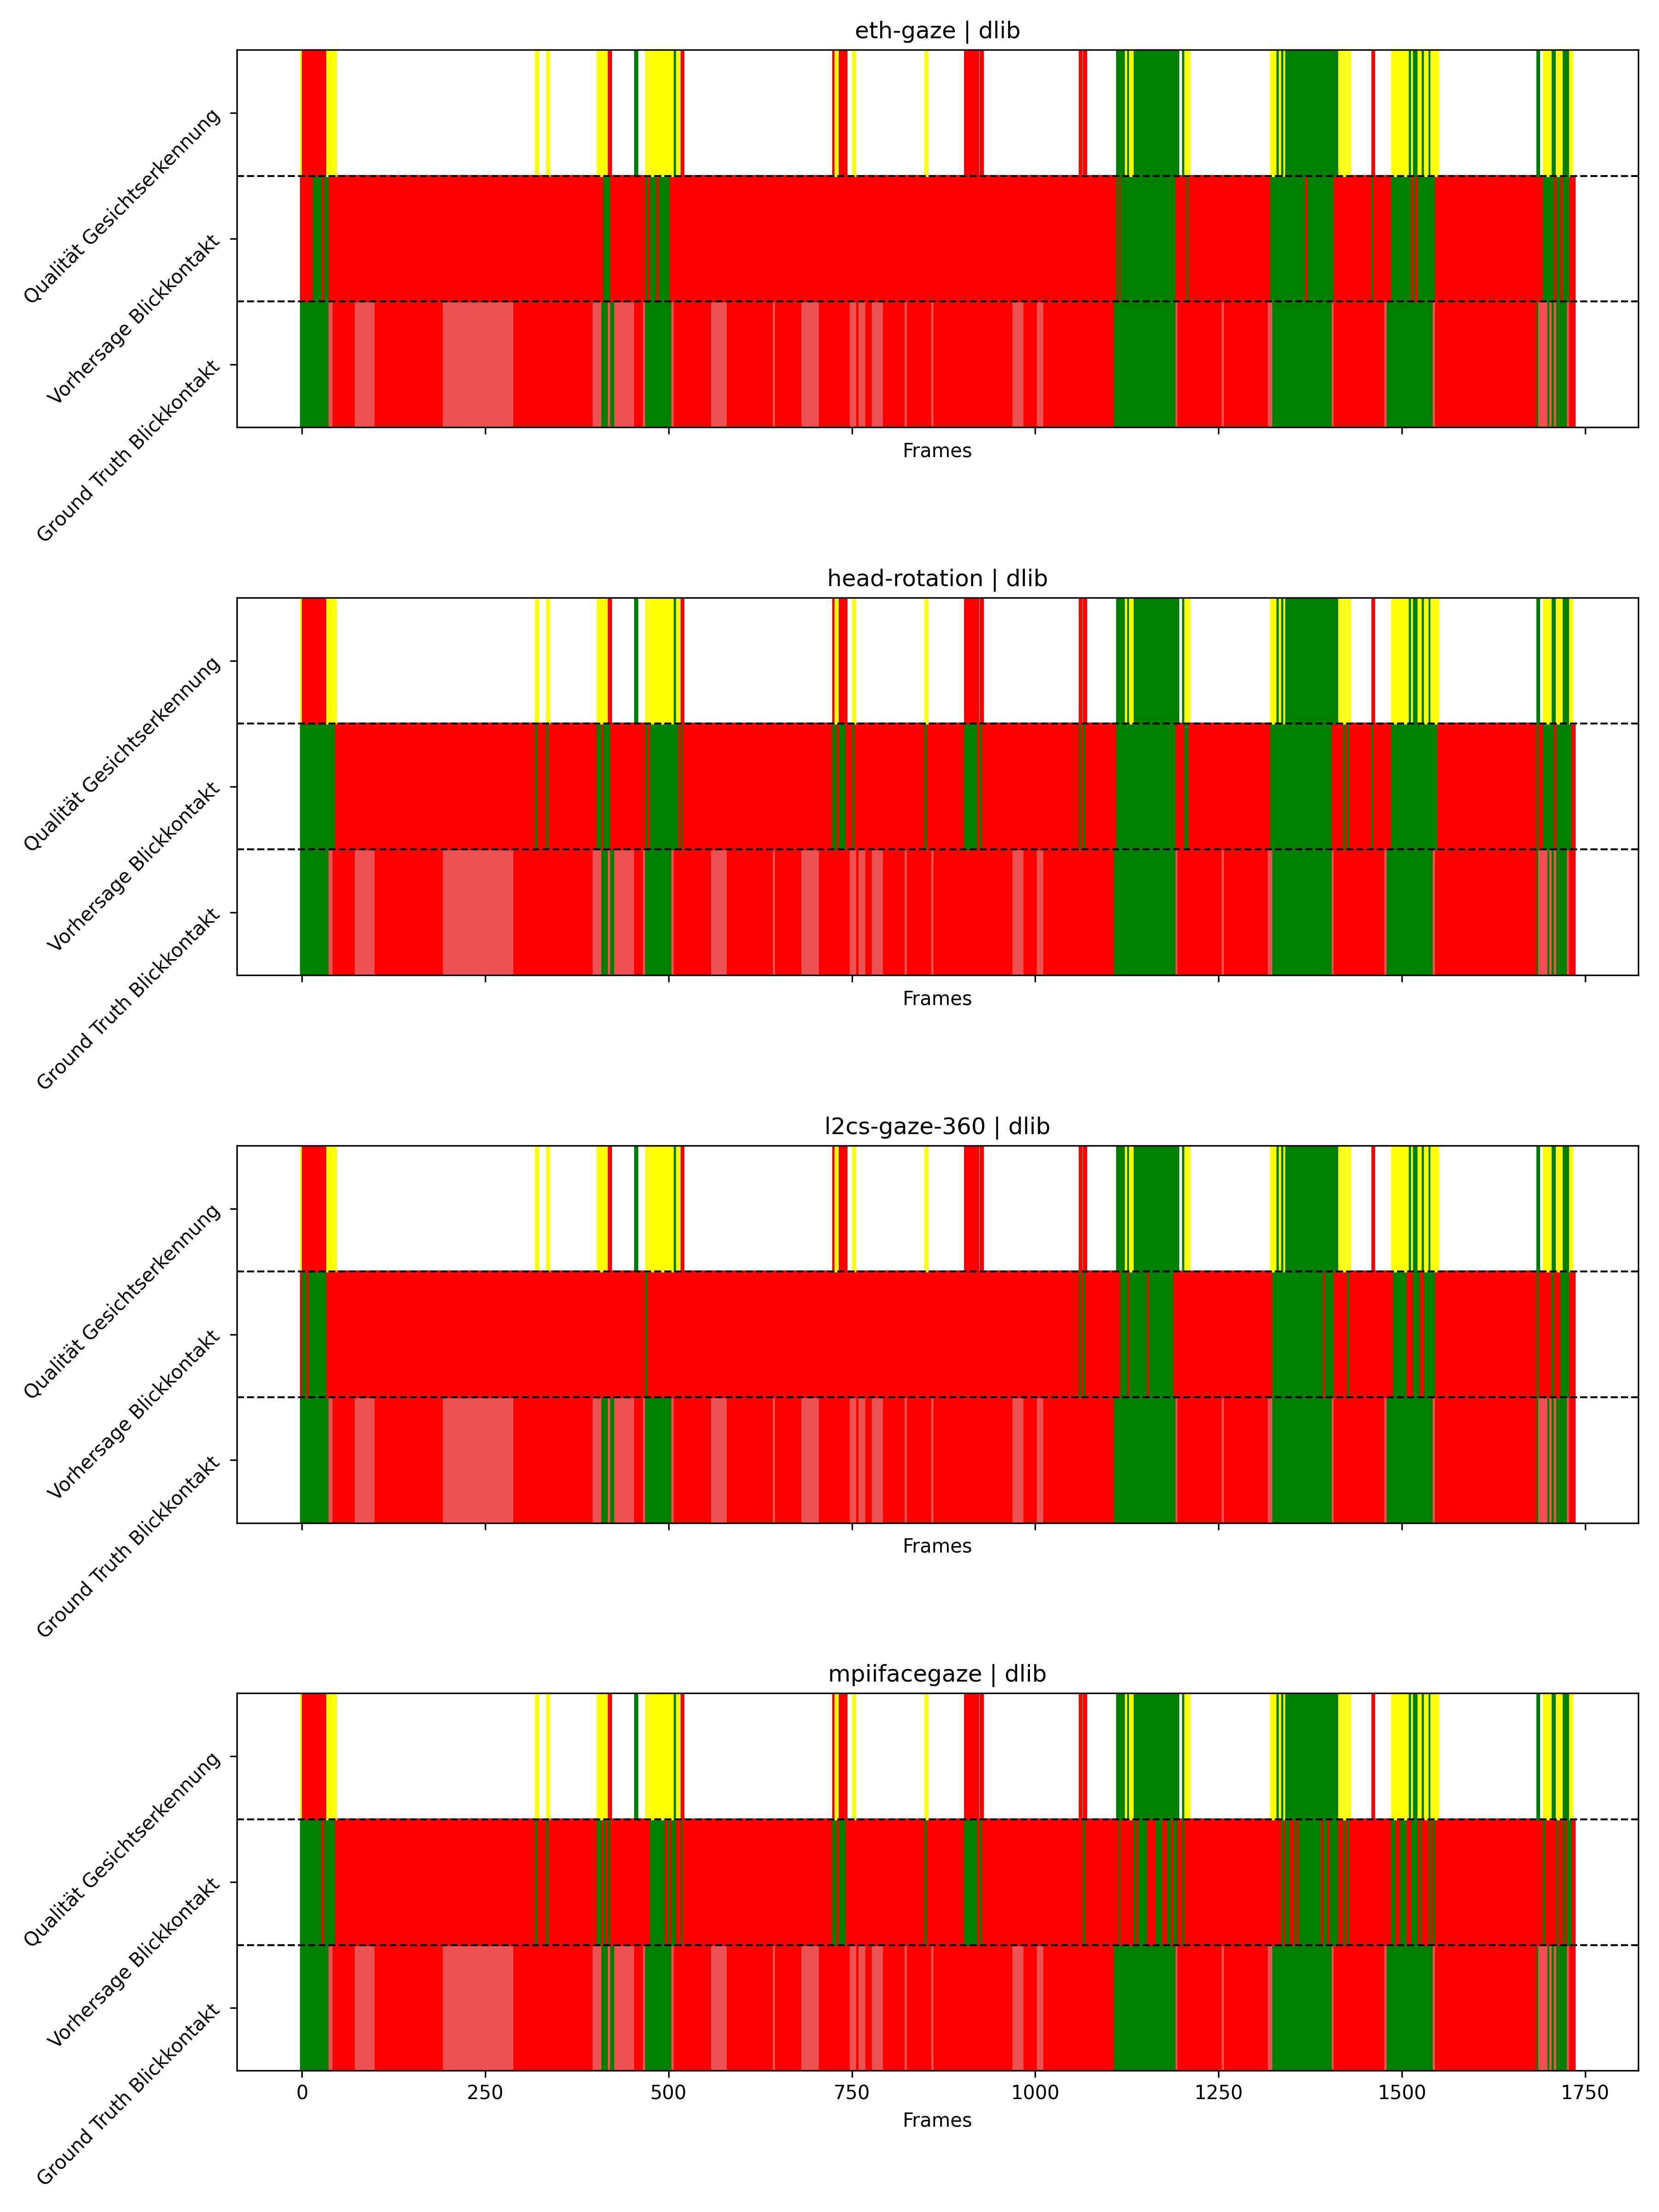
\includegraphics[width=1\linewidth]{appendix/24-dlib-overview-gaze.jpg}
\caption{Überblick über die Ground Truth des Blickkontakts, die Vorhersage des Blickkontakts und die Qualität der Gesichtserkennung mit \dlib. Die Bedeutung der Farben ist in Abbildung \ref{fig:evaluation:gaze:mpiifacegaze} erklärt.  }
\end{figure}

\begin{figure}[H]
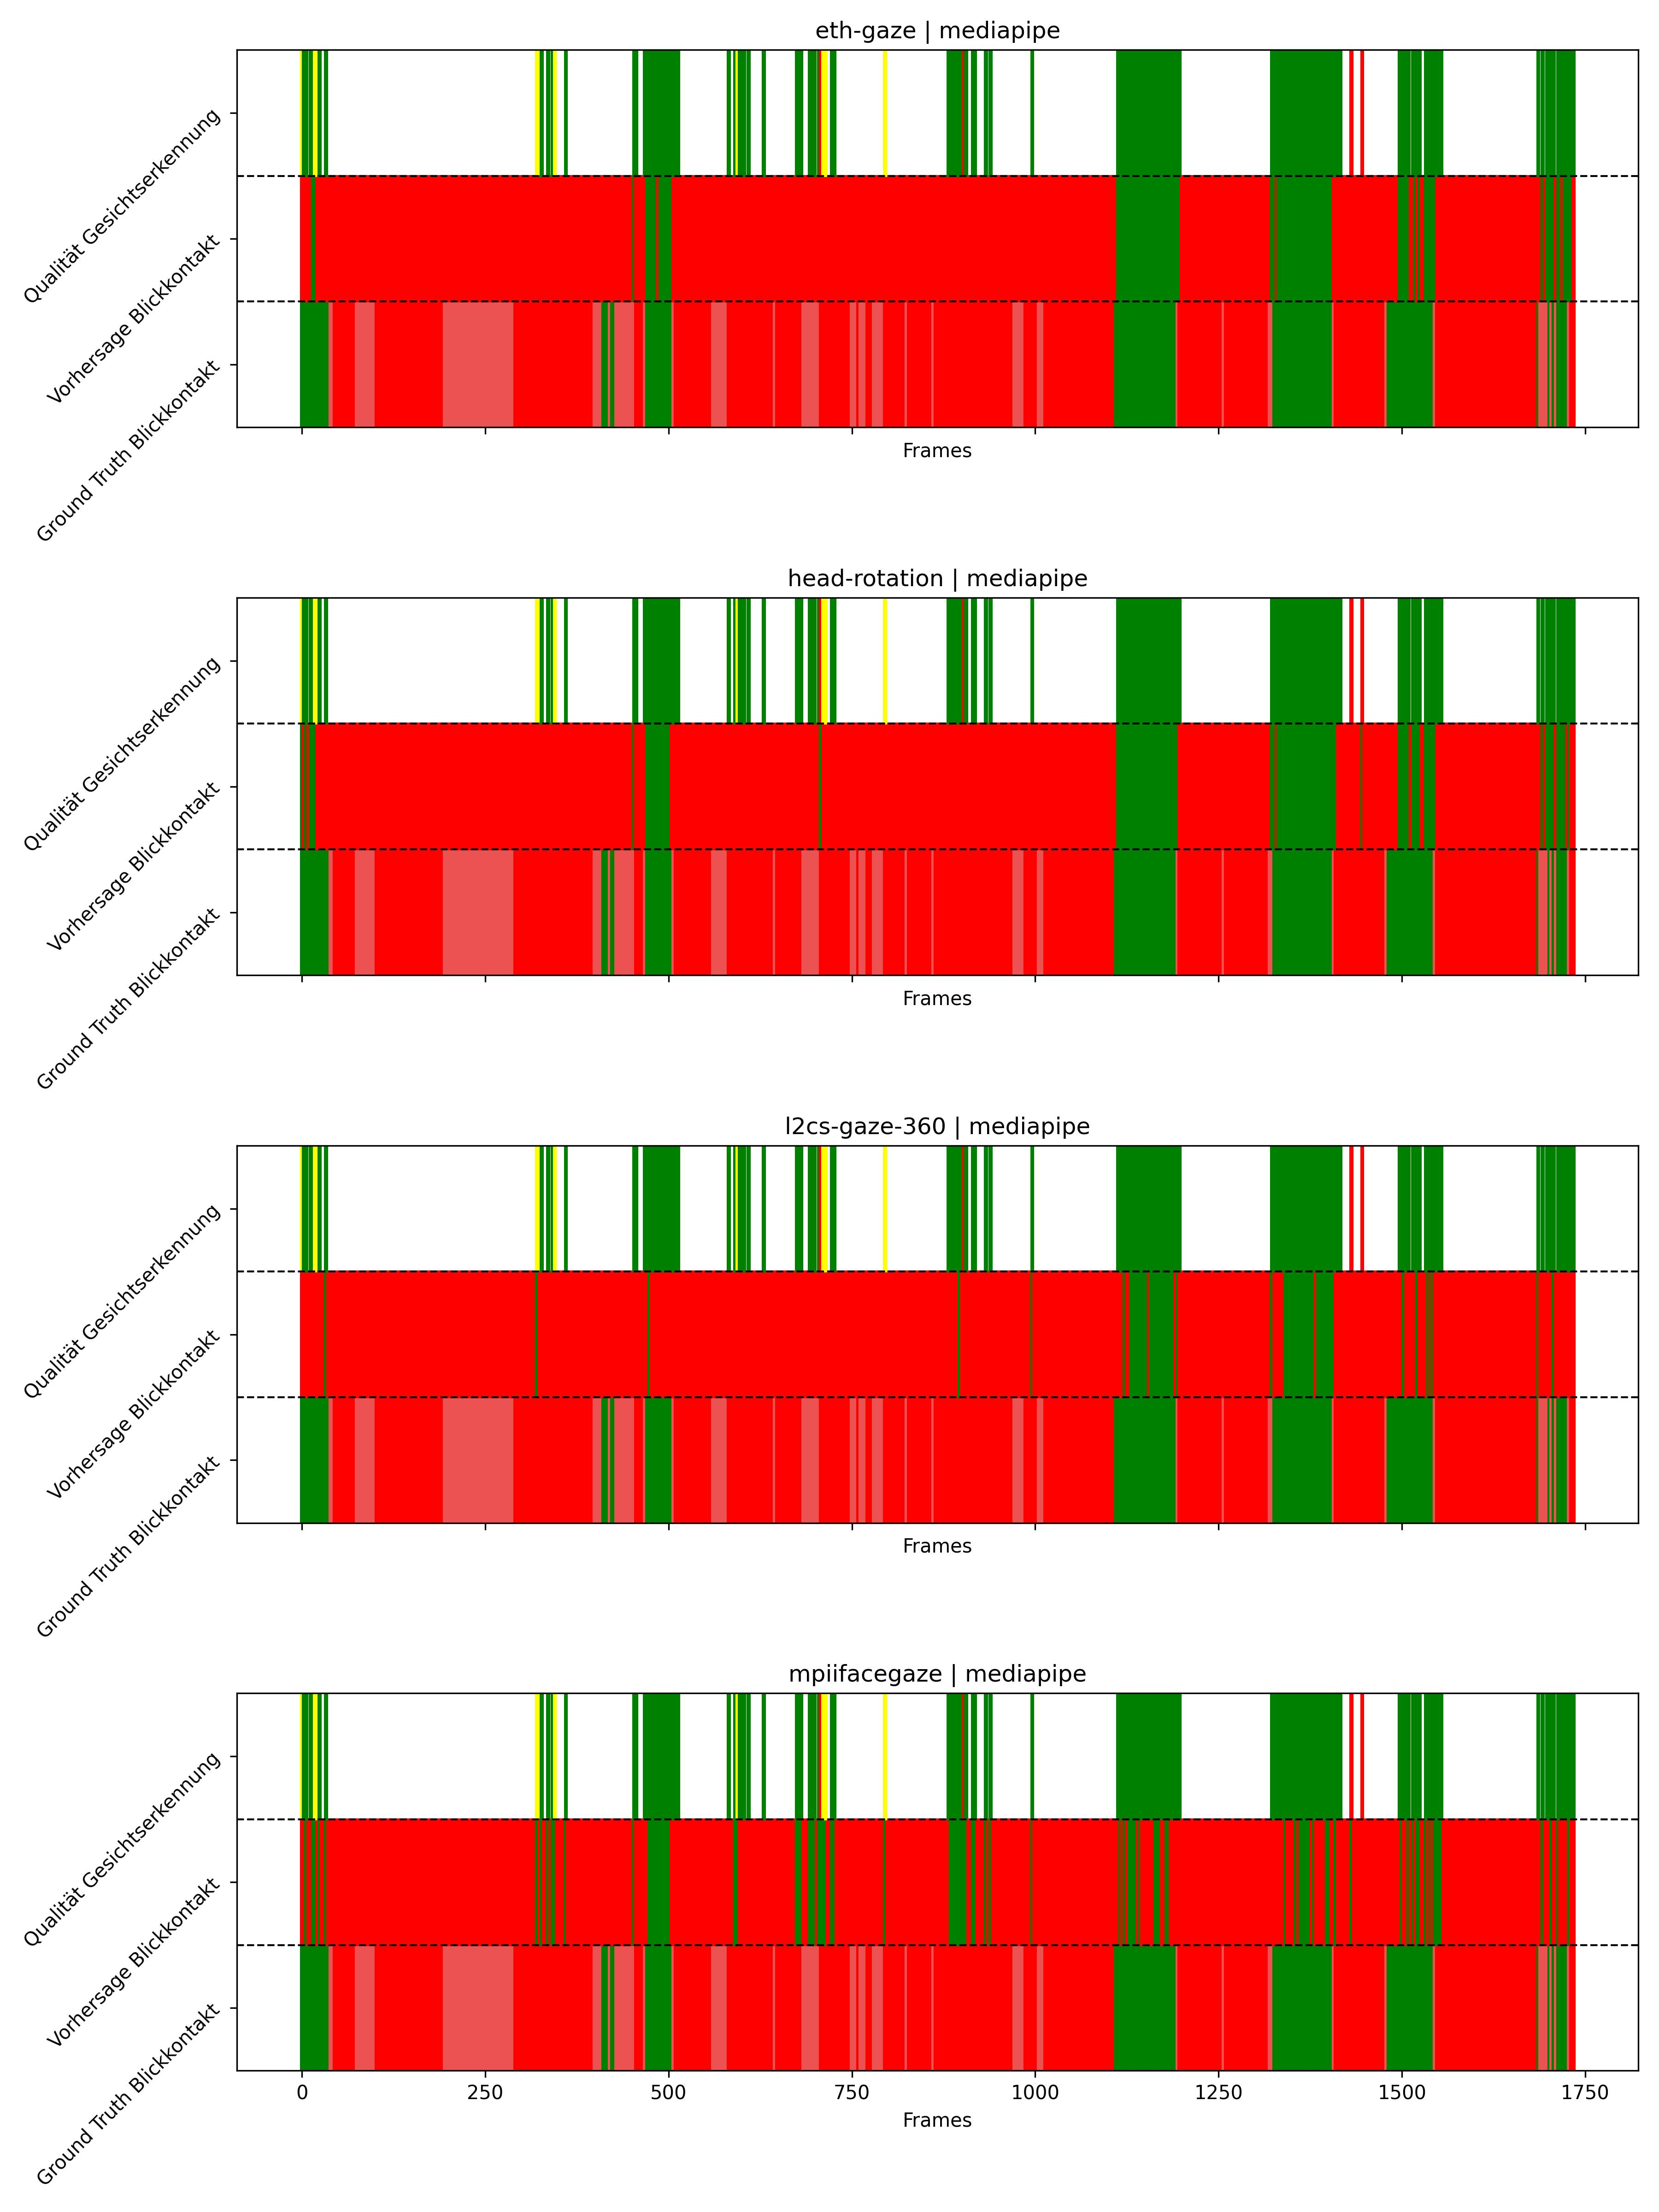
\includegraphics[width=1\linewidth]{appendix/24-mediapipe-overview-gaze.jpg}
\caption{Überblick über die Ground Truth des Blickkontakts, die Vorhersage des Blickkontakts und die Qualität der Gesichtserkennung mit \mediapipe. Die Bedeutung der Farben ist in Abbildung \ref{fig:evaluation:gaze:mpiifacegaze} erklärt.}
\end{figure}

